% Control file for Chet Hopp's PhD thesis

%Thesis outline control file, all elements declared within must be present locally
\documentclass[a4paper,12pt,twoside,openright,english]{book}

\usepackage{siunitx, booktabs, bm, longtable, multirow}
\usepackage{latexsym, syntonly, textcomp, amsmath, caption, float}
\usepackage{blindtext, setspace, rotating, afterpage, natbib, longtable}
\usepackage{array, abbrevs, titlesec, fancyhdr, sidecap, xcolor}
\usepackage{chngcntr, threeparttable, etoolbox, babel}

\usepackage[top=2.3cm, inner=3.2cm, bottom=2.3cm, outer=2.3cm]{geometry}
\usepackage[bookmarks]{hyperref}
\usepackage[toc,page]{appendix}
\usepackage[toc,acronym]{glossaries}


% \usepackage[hyphens]{url} %break line within long urls
%in tabular environment: cell of fixed width with wrapping and align left (L), centred (C), aligned right (R)
%manual breaklines with \newline
\newcolumntype{L}[1]{>{\raggedright\let\newline\\\arraybackslash\hspace{0pt}}m{#1}}
\newcolumntype{C}[1]{>{\centering\let\newline\\\arraybackslash\hspace{0pt}}m{#1}}
\newcolumntype{R}[1]{>{\raggedleft\let\newline\\\arraybackslash\hspace{0pt}}m{#1}}

% Title formatting
\titleformat{\chapter}{\Huge\bfseries}{\chaptername\ \thechapter}{0pt}{\vskip 20pt\raggedright}%
\titlespacing{\chapter}{0pt}{10pt}{<after-sep>}%

% Hyperlink setup here
\hypersetup{
    colorlinks=true,
    linkcolor={red!25!black},
    citecolor={blue!50!black},
    urlcolor={blue!80!black}
}

\pagestyle{fancy}

% Allow appendices within chapters
\AtBeginEnvironment{subappendices}{%
\chapter*{Appendix}
\addcontentsline{toc}{chapter}{Appendices}
\counterwithin{figure}{section}
\counterwithin{table}{section}
}
\numberwithin{figure}{chapter}
\numberwithin{table}{chapter}

% Here we ensure that the chapter and section
% headings are in lowercase.
	\renewcommand{\chaptermark}[1]{%
    	    \markboth{#1}{}}
	\renewcommand{\sectionmark}[1]{%
    	    \markright{\thesection\ #1}}
	\fancyhf{}  % delete current header and footer
	\fancyhead[LO,RE]{\bfseries\thepage}
	%\fancyhead[LO]{\bfseries\rightmark}
	%\fancyhead[RE]{\bfseries\leftmark}
	\fancyhead[LE]{\emph\textit{\nouppercase{\rightmark}}}
	\fancyhead[RO]{\emph\textit{\nouppercase{\leftmark}}}
	\fancyhead[RE]{}
	\fancyhead[LO]{}
	\fancyfoot[LE]{\thepage}
	\fancyfoot[RO]{\thepage}
	\renewcommand{\headrulewidth}{0.5pt}
	\renewcommand{\footrulewidth}{0.5pt}
	\addtolength{\headheight}{3pt} % space for the rule
	\fancypagestyle{plain}{%
   \fancyhead{} % get rid of headers on plain pages
   \renewcommand{\headrulewidth}{0pt} % and the line
		}

\makeindex
	%attempt to make chapter headings start higher up
	\titleformat{\chapter}[hang]{\LARGE\bfseries}{\thechapter}{1em}{}
	\titlespacing*{\chapter}{0pt}{0.7cm}{1.5cm}
	\titlespacing*{\section}{0pt}{0.7cm}{0.5cm}

% Load in glossary entries
\makeglossaries
% Acronyms and units
\newacronym{NAP}{NAP}{Nga Awa Purua}

\newacronym{RGEN}{RGEN}{Rotokawa A plant}

\newacronym{WHP}{WHP}{Wellhead Pressure}
 
\newacronym{DHP}{DHP}{Downhole Pressure}

\newacronym{II}{$II$}{Injectivity Index}

\newacronym{CFF}{CFF}{Central Field Fault}

\newacronym{IFF}{IFF}{Injection Field Fault}

\newacronym{PFF}{PFF}{Production Field Fault}

\newacronym{t/h}{t/h}{Tonnes per hour}

\newacronym{MWe}{MWe}{Megawatts electrical}

\newacronym{pdf}{pdf}{probability density function}

\newacronym{MPa}{MPa}{Megapascal}

\newacronym{TVZ}{TVZ}{Taup\={o} Volcanic Zone}

\newacronym{PTS}{PTS}{Pressure Temperature Spinner}



% Termz
\newglossaryentry{tracer_test}
{
    name=tracer test,
    description={Procedure in which a radioactive chemical compound, with known half-life, is injected into a reservoir. Production wells are monitored for the arrival of this compound, the arrival time and concentration of which can be used to infer flow properties of the reservoir.}
}

\newglossaryentry{WHP_g}
{
    name=wellhead pressure,
    description={Pressure in a well as measured at the wellhead, (approximately the earth's surface). Often reported in bar, but here converted to megapascal (MPa) as is the standard for seismology}
}
 
\newglossaryentry{DHP_g}
{
    name=downhole pressure,
    description={Pressure in a well as measured at a given depth by gas-filled tubing or an installed sensor. Often reported in bar, but here converted to megapascal (MPa) as is the standard for seismology}
}

\newglossaryentry{flow_rate}
{
    name=flow rate,
    description={The volume of fluid being injected into, or extracted from, a well per unit time. Reported in New Zealand as tonnes per hour (t/h)}
}

\newglossaryentry{II_g}
{
    name=injectivity index,
    description={A measure of a well's ability to accept a volume of fluid per unit pressure, here reported as t/h/MPa}
}

\newglossaryentry{injectivity}
{
    name=injectivity,
    description={Shorthand for injectivity index (II; above)}
}

\newglossaryentry{stimulation}
{
    name=stimulation,
    description={A prescribed treatment of a well intended to increase its permeability so that more fluid can be injected or extracted}
}

\newglossaryentry{permeability}
{
    name=permeability,
    description={The ability of a material to transmit fluid}
}

\newglossaryentry{transmissivity}
{
    name=transmissivity,
    description={The permeability\slash{thickness} product, typically reported from pressure transient tests}
}

\newglossaryentry{diffusivity}
{
    name=diffusivity,
    description={A quantity describing the rate at which fluid particles spread or diffuse. Reported as area per unit time (m$^{2}$ / s)}
}

\newglossaryentry{feedzone}
{
    name=feedzone,
    description={A location of significant permeability in a well. These are the locations into which fluid is inferred to enter or exit the reservoir}
}


%% XXXXXXXXXXXXXXXXXXXXXXXXXXXXXXXXXXX Document starts here XXXXXXXXXXXXXXXXXXXXXXXXXXXXXXXXXXXXXXXX

\begin{document}
\frontmatter

% Title page setup
\begin{titlepage}
\doublespacing
	\begin{center}
	\vspace*{2\baselineskip}
		\textbf{\LARGE{Characterizing microseismicity at Rotokawa and Ngatamariki geothermal fields
}}

		\vspace*{2\baselineskip}
		By \vspace*{2\baselineskip}
		Chet Hopp \vspace*{2\baselineskip}
 \vspace*{1\baselineskip}
\singlespacing
		A thesis\\ submitted to Victoria University of Wellington\\
		in fulfillment of the requirements for the degree of
		\\Doctor of Philosophy in Geophysics.\\
		\vspace*{3\baselineskip}
		Victoria University Wellington\\2019
  \end{center}
\end{titlepage}
\singlespacing
\clearpage{\pagestyle{empty}\cleardoublepage} %%no page number, which is wrong, on black page

% Stupid quotes page. Make a mockery of this.
\thispagestyle{empty} %suppress page number here without suppressing all page headers afterwards
  \begin{center}
		\emph{``I was doing plenty wrong, but they done wronger.''}\\
		\vspace*{1\baselineskip}
		Richard Petty
		
		\vspace*{4\baselineskip}
		\emph{``Don't point a gun at him. He's an unpaid intern.''}\\
		\vspace*{1\baselineskip}
		Steve Zissou
	\end{center}
\clearpage{\pagestyle{empty}\cleardoublepage}%hides page number which was wrong
\frontmatter

% Line spacing specification
\onehalfspacing

% Abstract page
%\ResetAbbrevs{all}
%\clearpage{\pagestyle{empty}\cleardoublepage}
%\pagestyle{plain}%restart page numbering
% \include{Abstract/Abstract_resubmitted}
% \include{Acknowledgements/Acknowledgements_resubmitted}

% Table of contents
\tableofcontents
\cleardoublepage
\listoffigures
\addcontentsline{toc}{chapter}{\listfigurename}
\listoftables
\addcontentsline{toc}{chapter}{\listtablename}

% Call chapter compilation here
\mainmatter
	%insert chapters here
	\cleardoublepage
	\cleardoublepage
	\chapter{Introduction}
\section{Motivation}
The heat present in the earth's crust has been recognized as a potential energy source for the generation of electricity for nearly a century, and has been exploited to this end for nearly 60 years in multiple locations \citep{Gregg_1958,GARRISON_1972,Minissale_1991}. To date, the worldwide installed geothermal capacity is over 14 gigawatts spread across more than 50 countries \citep{Pan_2019, Bertani_2016}, with the potential for substantially more through the creation of enhanced geothermal systems (EGS) \citep{Blackwell_2007}. Due to the confluence of abundant, naturally-fractured reservoirs, high heat flow and relatively low startup cost, New Zealand was one of the first countries to adopt geothermal as a source of electricity and currently has the fifth largest installed geothermal capacity in the world, accounting for roughly 16 percent of the nation's electricity generation \citep{Bertani_2016,Grant_2011}. However, the future growth of geothermal technologies is uncertain due to a number of associated risks including high startup costs \citep{Olasolo_2016} and the potential impact of induced seismicity (IS) related to injection and withdrawal of fluids \citep{Majer_2007,Ellsworth_2013}.

In the last decade, interest in IS has grown in the scientific and industrial communities as well as in the public sphere \citep{Ellsworth_2013}. Mostly, this is a result of the remarkable increase in seismicity in places such as Oklahoma, Arkansas, Texas and Ohio where wastewater from hydrocarbon production is being injected into the subsurface \citep[e.g.][]{Yeck_2017,Horton_2012,Kim_2013,McGarr_2017,Keranen_2013}. In addition, a number of geothermal projects have been abandoned or postponed due to the occurrence of larger-than-expected seismic events \citep[e.g.][]{Deichmann_2009,Grigoli_2018}. Given the incomplete understanding of the processes which generate such seismicity, it is difficult to reliably forecast its extent, magnitude and timing for a given injection or extraction scenario. However, these processes likely include injection parameters such as pressure, \gls{flow_rate}, temperature, total volume and proximity to basement formation, as well as reservoir properties like temperature, \gls{permeability}, volume, structure and in situ stress state \citep{Segall_1998,Bachmann_2012,Ellsworth_2013,mcgarr2014maximum,Jeanne_2015tensor,Goebel_2018}. As public and regulatory scrutiny of IS increases, it will become increasingly important to understand the detailed interactions between each of these factors in order to design strategies to mitigate the risk of generating large, damaging earthquakes \citep[e.g.][]{Langenbruch_2017}.

When viewed from a different perspective, the occurrence of human-induced seismicity presents a unique setting in which earthquakes can be observed at locations and times which are fully or partially known a priori. The ability to generate seismicity through controlled, measurable actions  offers us the opportunity to study, in great detail, the processes that lead to seismogenesis \citep[e.g.][]{Raleigh_1976}. These results can then be applied more widely to problems of natural (and often more damaging) seismicity.

Lest we forget that injection operations serve a purpose other than generating earthquakes, datasets of IS contain useful information regarding reservoir properties such as flow pathways, \gls{permeability} distribution and fracture geometry. From an operational standpoint, this information is critical in managing a dynamic resource like a geothermal reservoir \citep{Majer_2007}. This final point is the key to the work presented in this thesis.

In this work, we focus on the Ngatamariki and Rotokawa geothermal fields in the \acrfull{TVZ} on the North Island of New Zealand, from mid-2012 until the end of 2015. Both fields are exclusively operated by Mercury NZ, Ltd. The catalog of seismicity we have created is an indicator of processes occurring within the reservoirs that are otherwise difficult to measure without drilling additional wells (and spending significantly more money). These catalogs offer clues to the orientation and size of the fracture network, geometry of flow pathways, reservoir \gls{transmissivity}, and stress state in the reservoir. This insight is especially useful where reservoir behavior cannot be fully explained by borehole-based measurements.

\section{Geothermal Power}
\subsection{Power Production}
Geothermal electricity generation relies on converting the heat energy from the earth to mechanical energy, which is used to turn a generator. Heat is extracted from the subsurface through extraction of a conductively-heated gas or liquid phase from the reservoir rock. Therefore, a commercially viable geothermal resource requires high temperature (at accessible depths via rotary drilling) and sufficient \gls{permeability}, in order to enable rapid transport of fluid to the wellbore. As a general rule, the temperature of the earth's crust increases with depth at an average of 30\textdegree{C}\slash{km} \citep{Grant_2011}. On a more localized level, however, gradients of 100\textdegree C or greater can be encountered \citep{Grant_2011}. All modern, produced geothermal fields are convective systems, meaning that the pressure and temperature distribution in the field is governed not by conductive heat transfer, but by the circulation of hot fluids through permeable rock \citep{Grant_2011}. These types of fields can be broken into two basic types: liquid-dominated and vapor-dominated (of which there are few), based on the dominant fluid phase present in the reservoir. Both Ngatamariki and Rotokawa are liquid-dominated reservoirs \citep{McNamara_2016,Chambefort_2016}.

There are a variety of field configurations, but most modern geothermal fields consist of a production field, where fluid is drawn out of the reservoir, and an injection field where some portion (up to nearly 100 percent) of the extracted fluid is reinjected back into the reservoir. This is done for a number of reasons, the most important of which is to maintaining reservoir pressure and volume to avoid degrading the resource \citep{Grant_2011}. The injection and production field are connected via the power plant (or multiple plants) that uses the extracted fluid either directly or indirectly (i.e. a binary plant) to turn a turbine and generate electricity. There are many variations on the heat-to-electricity conversion system, and the choice of which to use at a particular field is governed by the dominant fluid phase in the reservoir and the reservoir temperature \citep{DiPippo_2016}. For the purposes of this thesis, we are concerned with binary (Figure \ref{nga_plant}), flash-steam (Figure \ref{rot_plants}a) and combined-cycle (Figure \ref{rot_plants}b) power plants, which are the types of plants installed at Ngatamariki and Rotokawa. A binary plant uses the fluid extracted from the reservoir to boil a highly-volatile, secondary fluid (for example, isopentane) with a much lower boiling point than the reservoir fluid, which is then used to turn a turbine. A flash steam plant, on the other hand, flashes the extracted reservoir fluid to steam, which is directly deployed in the turbine \citep{DiPippo_2016}. Combined cycle plants use both technologies simultaneously.

Two power plants are installed at Rotokawa. The first, a 24 \acrfull{MWe} combined-cycle plant (\acrfull{RGEN}), was installed in 1997, while the second, a 140 \acrshort{MWe}, triple-flash plant named \acrfull{NAP}, was installed in 2010 \citep{McNamara_2016}. Ngatamariki is the most recently-developed field in New Zealand, with the 82 \acrshort{MWe} binary power plant coming online in 2013.\selectlanguage{english}

\begin{figure}[h!]
\begin{center}
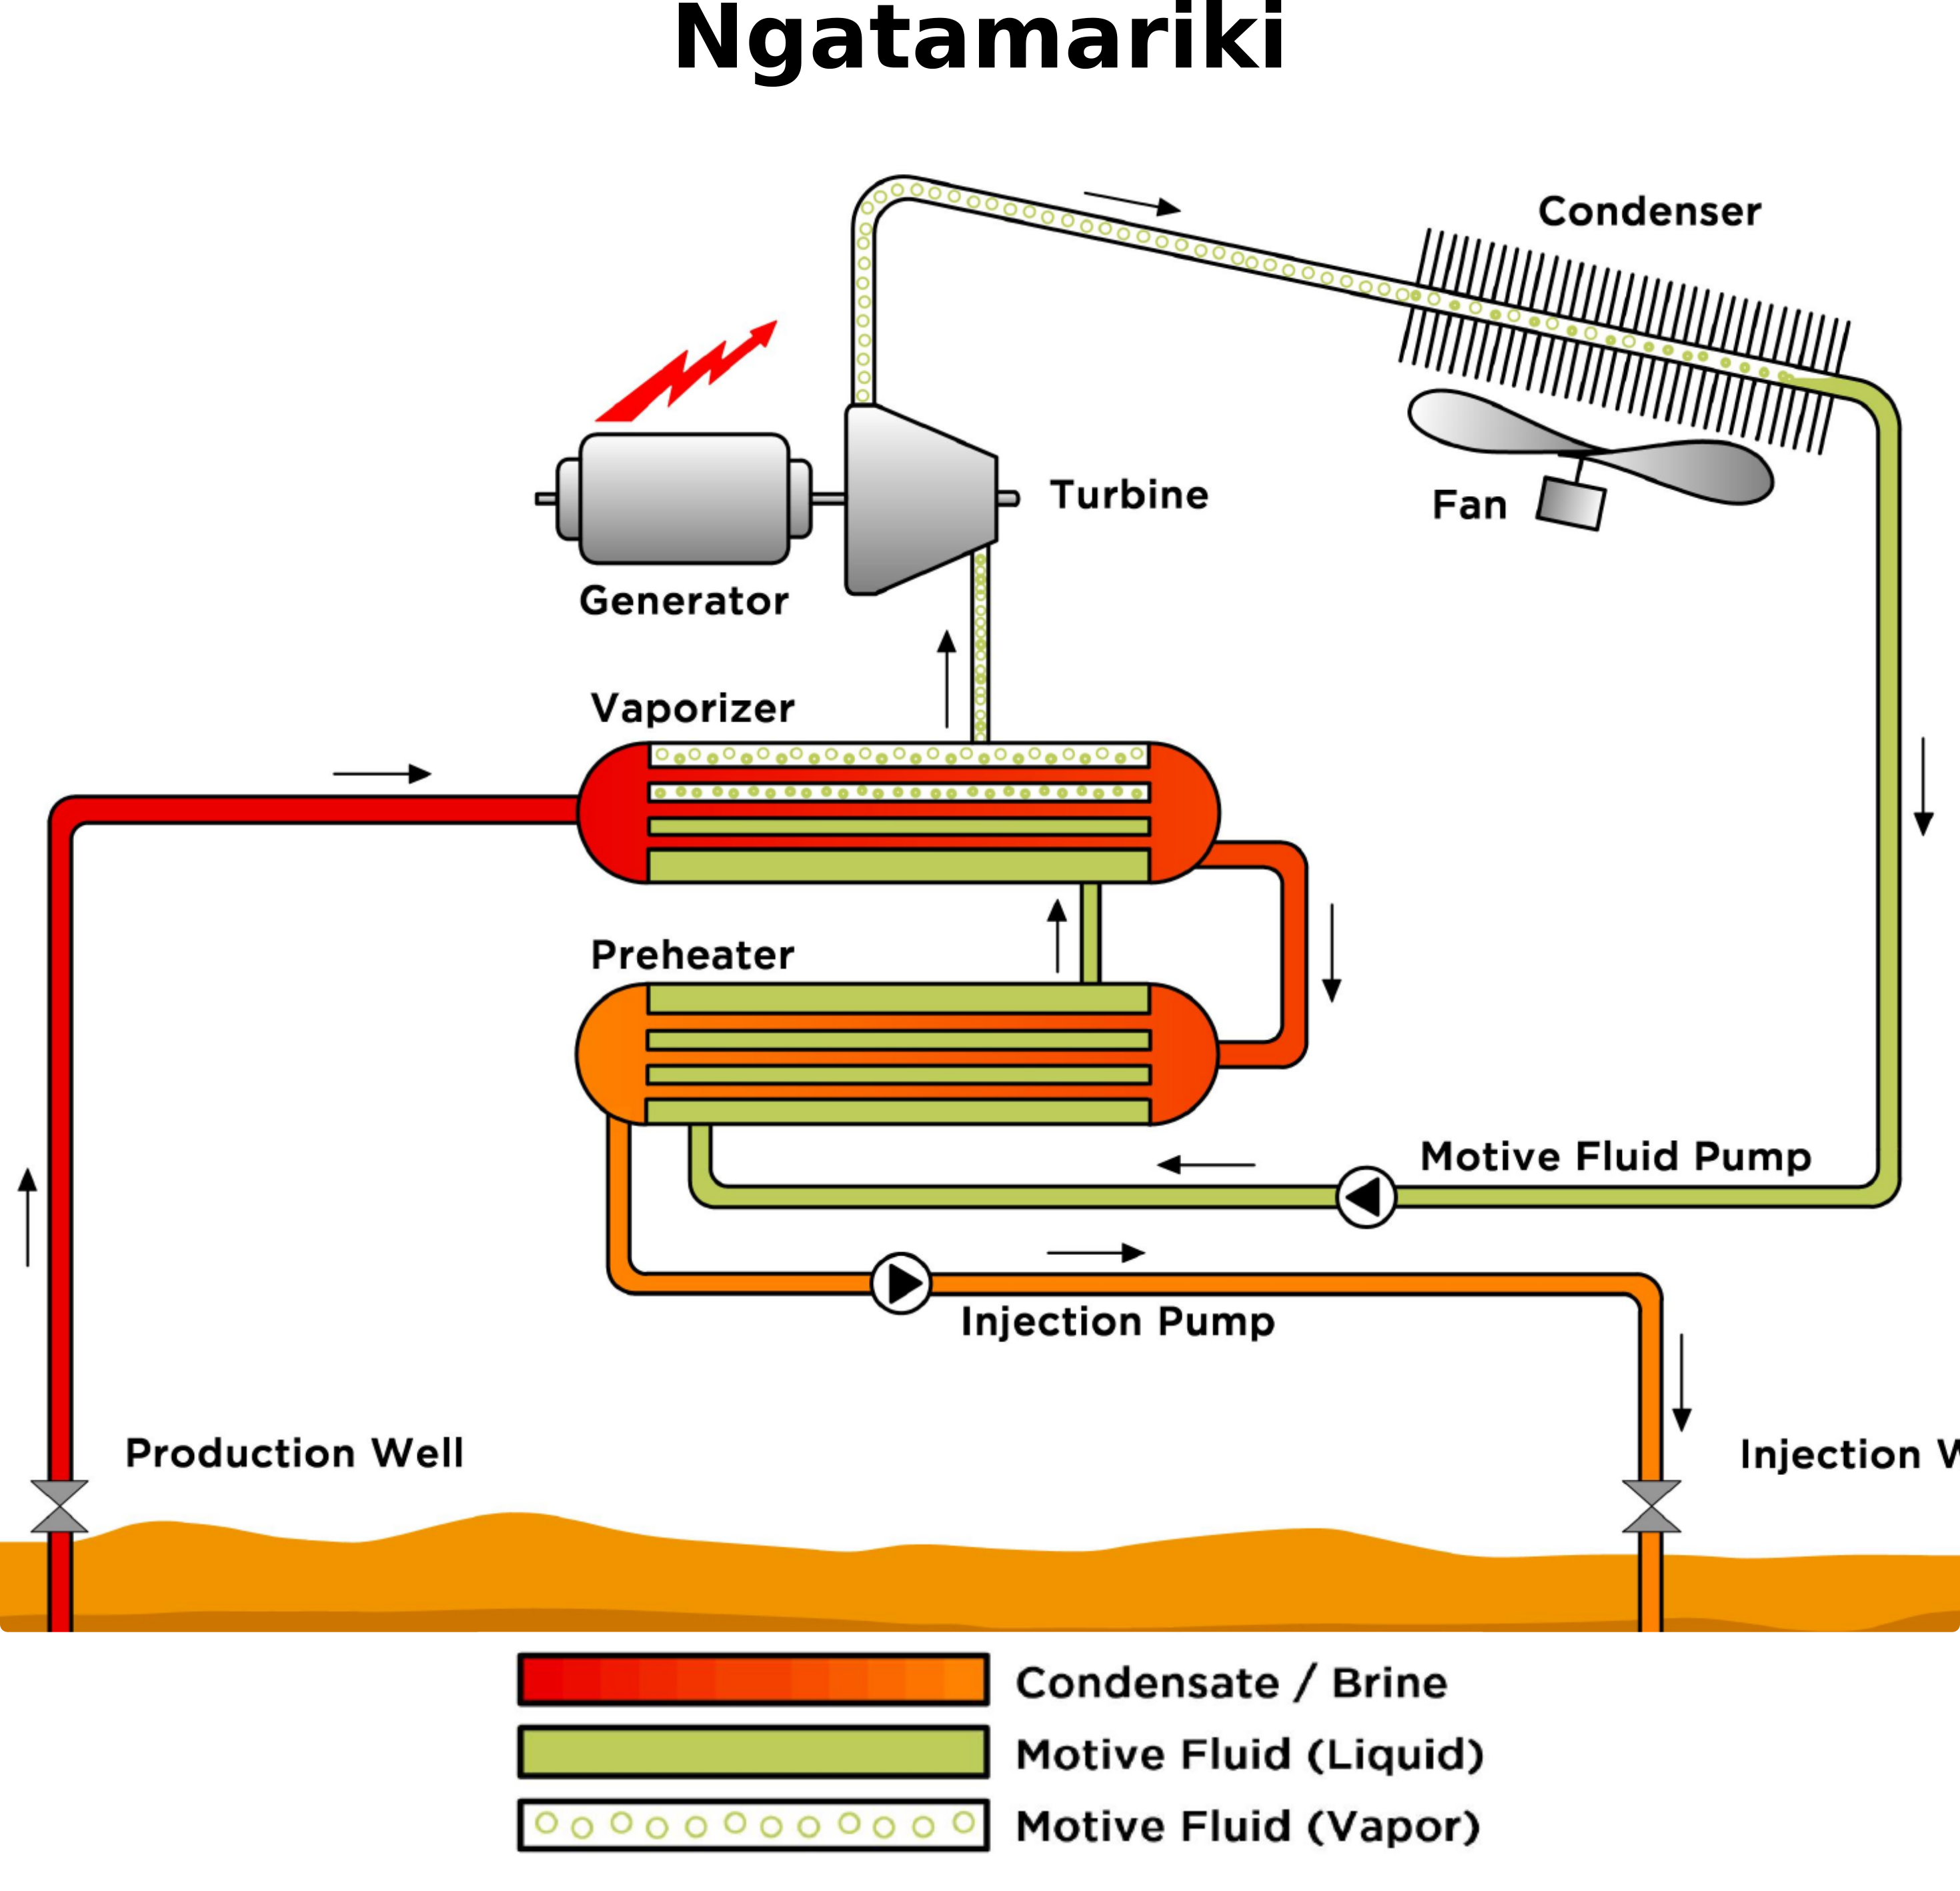
\includegraphics[width=\columnwidth]{Chapter_1_Intro/figures/ORMAT_techs_overview/Ngatamariki_schematic}
\caption[Schematics diagram of the Ngatamariki geothermal power plant design]{{
Schematic of the operation of a binary power plant, similar to the plant installed at Ngatamariki. This figure is adapted from the Ormat 2017 Annual Report \citep{Ormat_2018}.
{\label{nga_plant}}%
}}
\end{center}
\end{figure}

\begin{figure}[p]
\begin{center}
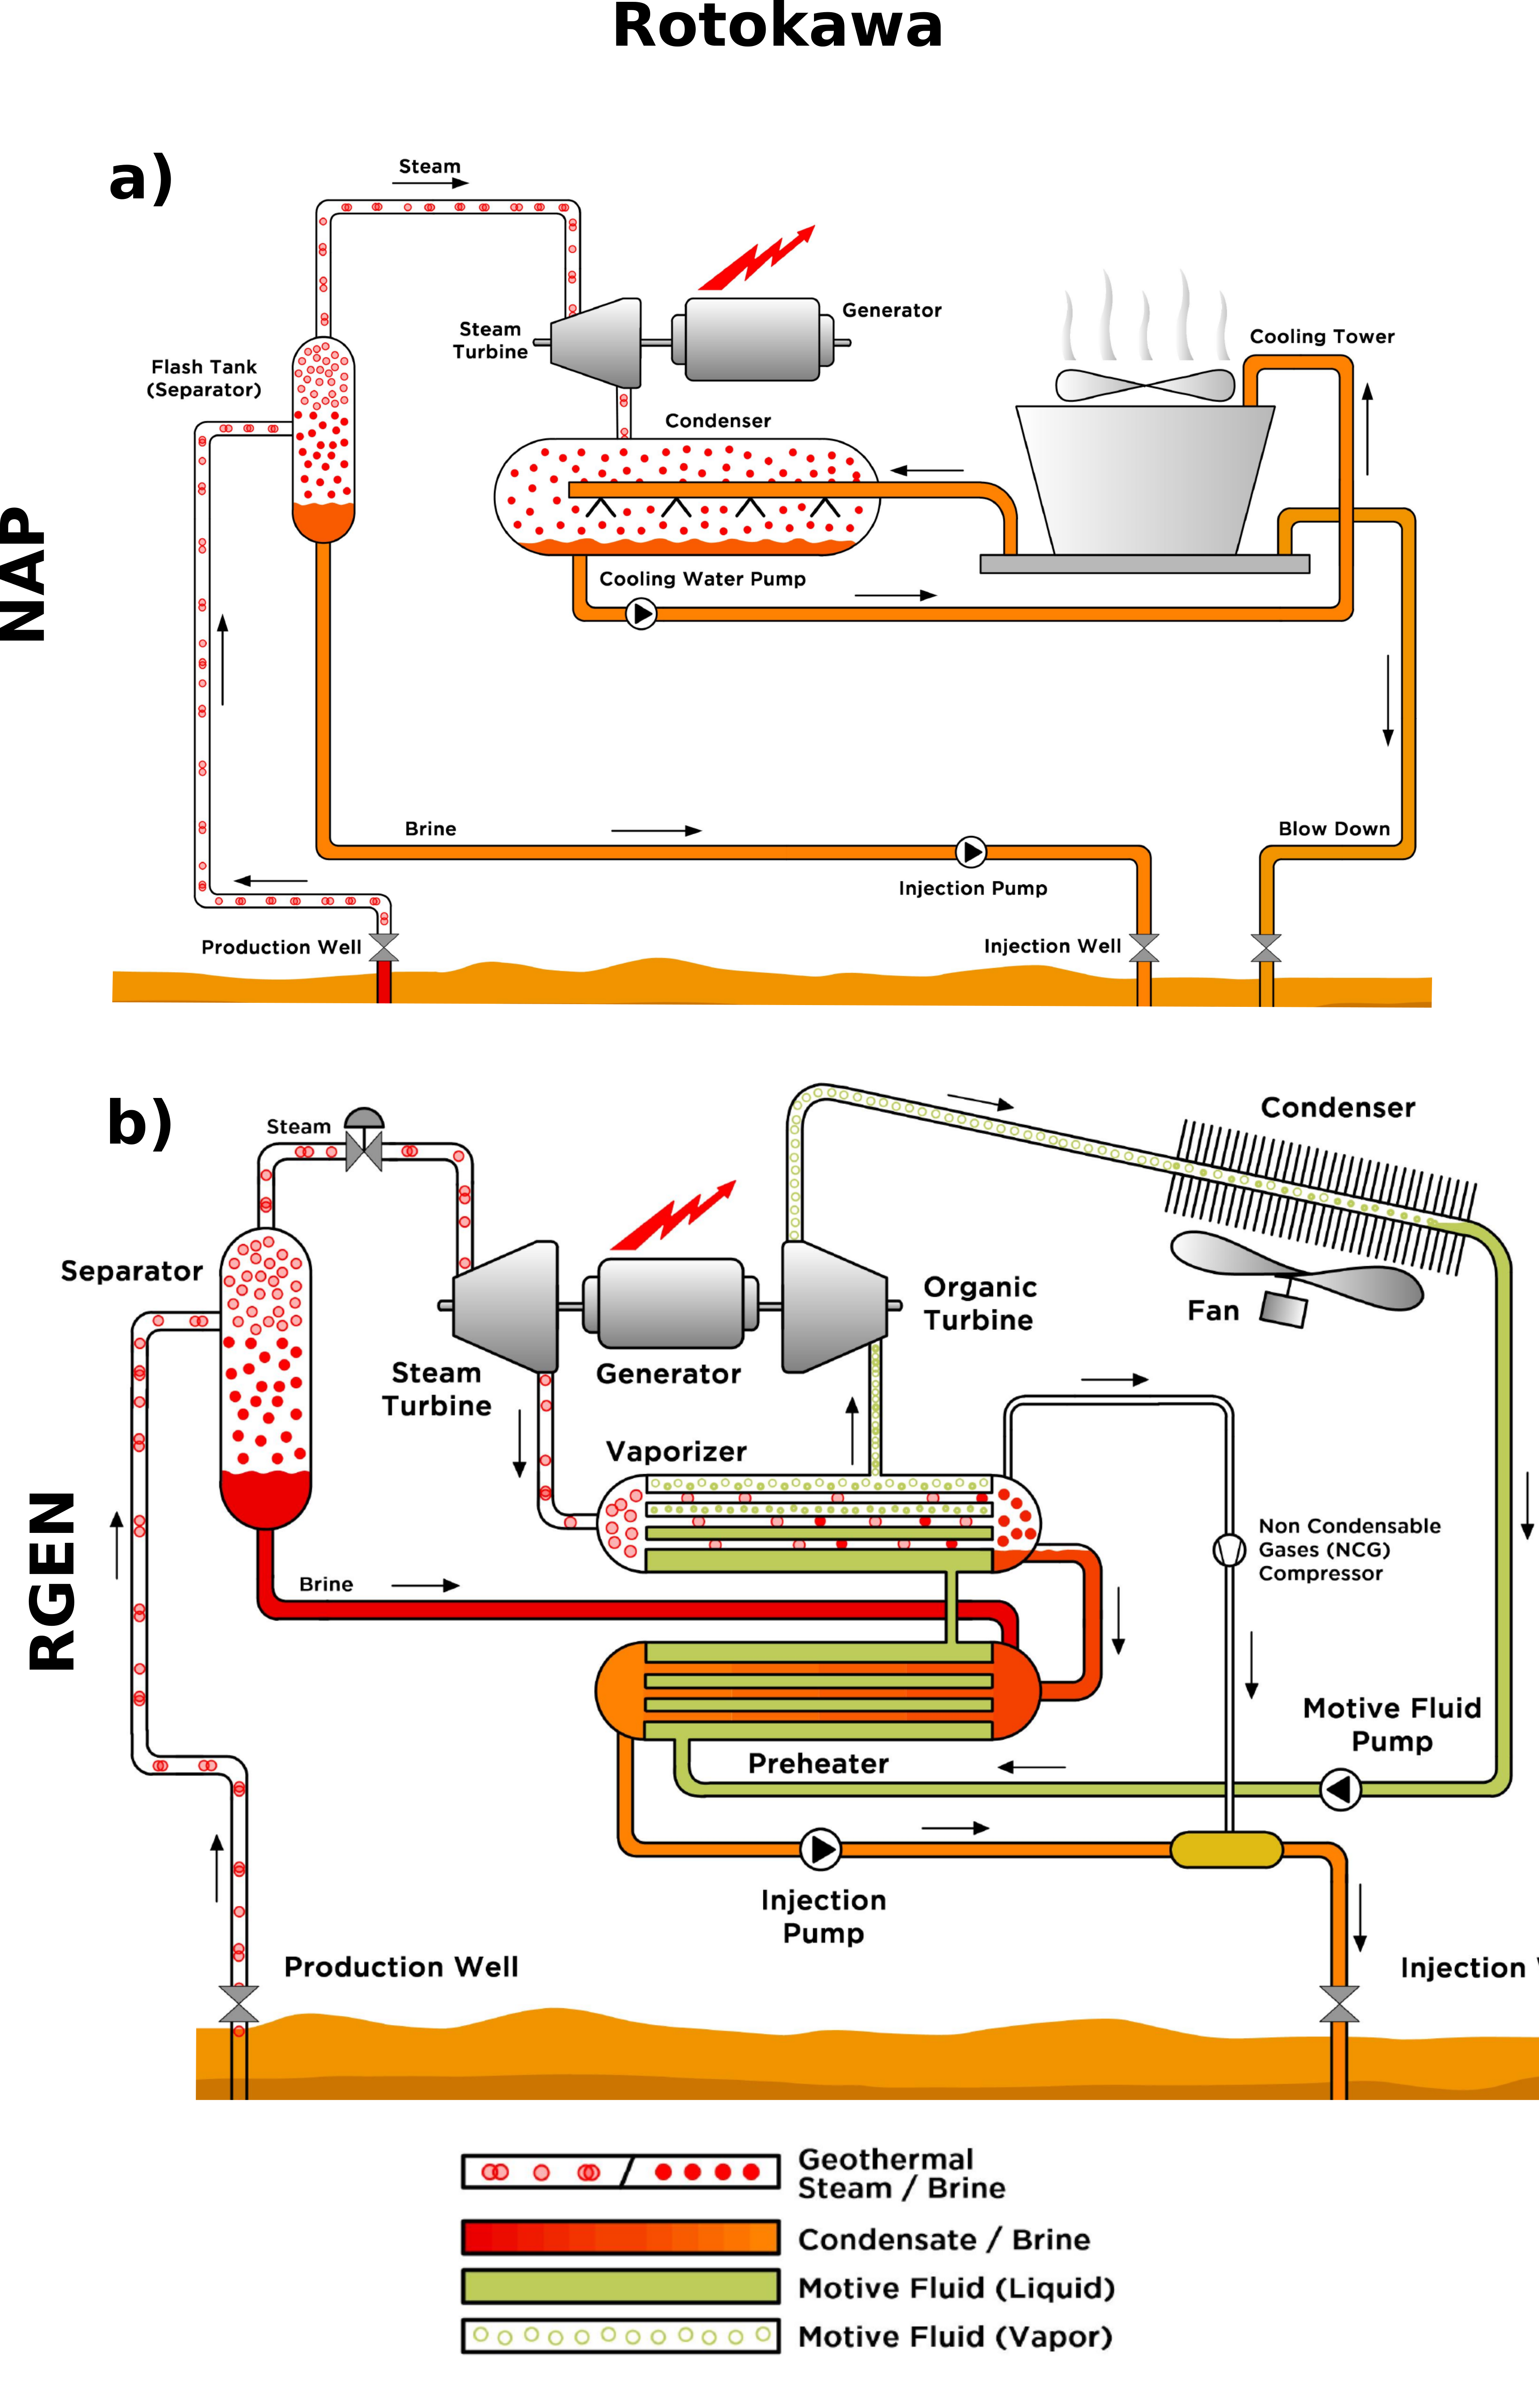
\includegraphics[width=0.85\columnwidth]{Chapter_1_Intro/figures/ORMAT_techs_overview/Rotokawa_schematic}
\caption[Schematic diagrams of Rotokawa geothermal power plant design]{{
Schematics diagrams showing the operation of the two types of geothermal power plants in operation at Rotokawa: a) Flash-steam and b) Combined cycle. At Rotokawa, the
original \acrfull{RGEN} is type b), while the more recently-installed \acrfull{NAP} plant is a `triple-flash' variant of type a), meaning that
there are three separate stages of liquid-steam separation, which
increases plant efficiency~\protect\cite{DiPippo_2016}. These figures are adapted from the Ormat 2017 Annual Report~\protect\cite{Ormat_2018}
{\label{rot_plants}}%
}}
\end{center}
\end{figure}

\section{Reservoir Management}
\subsection{Datasets}
Reservoir engineers, modelers, geologists and geophysicists use a number of data streams to assess the state of a given geothermal reservoir. Most of these data are recorded at boreholes drilled into the resource, and provide a wealth of important information \citep{DiPippo_2016,Grant_2011}. These data include:
\begin{itemize}
  \item{Geologic core}
  \item{Natural-state temperatures}
  \item{ \acrfull{PTS} data, collected by an impeller lowered down the wellbore}
  \item{Image logs (Fracture orientation/aperture/spacing and borehole breakout)}
  \item{Resistivity, porosity, density logs}
  \item{Injection and production \gls{flow_rate}}
  \item{Injection and production pressures}
  \item{Injection temperature and chemistry}
  \item{Radioactive \glspl{tracer_test}}
\end{itemize}
These datasets allow operators to constrain the spatial extent, temperature distribution and \gls{permeability} in the reservoir. However, they are sparsely sampled relative to the total reservoir area due to the prohibitive cost of drilling deep wells. To aid in interpreting the data listed above, other geophyisical and geochemical data are often collected at the surface, which include:
\begin{itemize}
  \item{Magnetotelluric surveys}
  \item{Microgravity surveys}
  \item{Leveling (subsidence monitoring)}
  \item{Spring/fumarole temperature and chemistry}
  \item{Active-source seismic}
  \item{Passive-source seismic}
\end{itemize}

Passive-source seismic data occupy a unique place in the spectrum of data available to geothermal operators. While waveform data are collected at the surface (or in some cases at 100s of meters depth in boreholes), they are the surface manifestation of fracture rupture (i.e. strain) at depth in the reservoir, a process that is affected by the distribution of reservoir temperature and pressure. Pressure and temperature can be accurately measured at wells, but seismicity can occur throughout a reservoir and it therefore gives a much more densely-sampled view of fluid movement at depth. For the purposes of this thesis, we will focus on the characterization of reservoir seismicity and its relation to many of the well parameters listed above. The most important constraints on the state of the reservoir come from well pressure and flow rate data, both of which will feature prominently in the work that follows. 

\subsection{Terms and Definitions}\label{terms}

When assessing the relationship between seismicity and reservoir management, we generally focus on injection, as opposed to production. This is mostly because the withdrawl of fluids decreases pore-fluid pressure and, therefore, usually stabilizes reservoir fracture networks \citep{Segall_1994,Segall_1998}(see further discussion in Section \ref{mechanisms}). However, not all injection operations are the same, and each has a specific set of goals that will be important to understand in the context of IS at Rotokawa and Ngatamariki:
\begin{itemize}
  \item{\textbf{Reinjection}}
  
  During the normal operation of a power plant, brine is extracted from the reservoir, put through the power plant, and reinjected. This type of operation makes up the bulk of the reinjection operations in our dataset. In the case of the two fields considered here, brine reinjection is characterized by high flow rates (up to $\sim$1000 t/h), high temperatures ($\sim$90\textdegree C) and an injectate chemistry consistent with that of the reservoir fluid. Flash plants also produce a significant amount of condensate, which is the liquid product of the cooling of steam. Most geothermal plants produce this in some form and it must also be reinjected into the reservoir, albeit with a lower temperature (ambient to $\sim$40\textdegree{}C) than brine and with a chemical composition similar to river water.
  \item{\textbf{Completion Testing}}
  
  Once a well has been drilled, engineers and modelers need to be able to estimate the extent and \gls{permeability} of the reservoir in order to better estimate its future behavior. To do this, completion tests are conducted by varying the flow rate into (or out of) the well, and measuring the resulting pressure response \citep{horne1995modern}. At Ngatamariki, completion testing was done with river water ($\sim$15\textdegree C) at flow rates of up to 200 t/h.
  \item{\textbf{Stimulation Testing}}
  
  Stimulation testing refers to the injection of fluid with the express purpose of measuring the change in the \gls{permeability} of the well. This is important, as the flow rates during injection testing are usually much lower than those required to run the power plant to its full capacity. In the case of a binary plant (Figure \ref{nga_plant}) where the geothermal fluid circulates through the system in a closed loop, the operator needs to be able to reinject nearly 100 percent of this extracted volume. Therefore, an estimation of the potential of a well to accept increasing volumes of fluid is essential in accurately modeling the feasibility of the entire power scheme once the plant comes online \citep{DiPippo_2016,Grant_2011}.
  
  In high-temperature geothermal reservoirs, stimulation is likely associated with thermal contraction of the walls of the fractures though which fluid is flowing \citep{grant2013thermal}, which may manifest as aseismic opening of the fractures \citep[e.g.][]{Guglielmi_2015}. However, stimulation may also be related to seismic slip on fractures through which \gls{permeability} can be either increased or decreased, an effect which has been extensively studied in the lab and through numerical simulations \citep[e.g.][and references therein]{Lee_2002,Fang_2017}. See Section \ref{mechanisms} for further discussion of stimulation and \gls{permeability} changes.
\end{itemize}

With these injection scenarios in mind, it will be useful to define at the outset of this thesis certain basic terms and quantities that we will lean on in the following chapters:
\begin{itemize}
  \item{\acrfull{WHP}}
  \item{\acrfull{DHP}}
  \item{\Gls{flow_rate}}
  \item{\acrfull{II}}
  \item{\Gls{stimulation}}
  \item{\Gls{permeability}}
  \item{\Gls{transmissivity}}
  \item{\Gls{diffusivity}}
\end{itemize}

Measuring reservoir pressure is of paramount importance to assessing the state of the resource. This quantity can be measured in the well at or near the depth of the reservoir, in which case the measurement is referred to as \gls{DHP_g} (\acrshort{DHP}). If the pressure measurement is taken at the wellhead (\gls{WHP_g}, \acrshort{WHP}), however, some basic corrections need to be made to estimate the reservoir pressure at depth. Assuming a static water column in the well:

\begin{equation}
WHP = P_{r} - \rho{g}Z
\end{equation}

where $P_{r}$ is the reservoir pressure and $\rho{g}Z$ is the weight of the water column at depth $Z$. However, if the well is flowing, as is generally the case for wells in a geothermal field \citep{grant2013thermal,Clearwater_2015}:

\begin{equation}
WHP = P_{r} - \rho{g}Z + \frac{W}{II} + KW^{2}
\end{equation}

Where $W$ is mass \gls{flow_rate} (typically measured in tonnes per hour in New Zealand) and $KW^{2}$ is a term accounting for the frictional forces related to fluid flow down the well. \acrshort{II} is the \gls{II_g}, typically referred to simply as \gls{injectivity}, which is a measure of the well's ability to accept fluid at a given pressure. The \acrshort{II} relationship is calculated as \citep{DiPippo_2016}:

\begin{equation}
II = \frac{W}{P_{w} - P_{r}}
\end{equation}

where $P_{w} - P_{r}$ is the difference in pressure between the well and reservoir (overpressure). The increase in \acrshort{II} is typically referred to as `\gls{stimulation}', which can be thought of as an increase of the \gls{permeability} of a well. Geothermal operators typically `stimulate' both production and injection wells once they have been drilled in order to increase the amount of fluid that can be drawn out of, or put into, the reservoir prior to plant startup.

\citet{grant2013thermal} suggest that geothermal wells stimulate as a power of time according to the empirical relationship: $II = Ct^{n}$ where $C$ is a constant, $t$ is time since the start of injection and $n$ has a value between 0.3 and 0.7 for the wells considered in their study. Figure \ref{415417} shows this relationship during the stimulation of NM08 at Ngatamariki \citep{Clearwater_2015}, which stimulated according to $n\approx0.7$.\selectlanguage{english}

\begin{figure}[h!]
\begin{center}
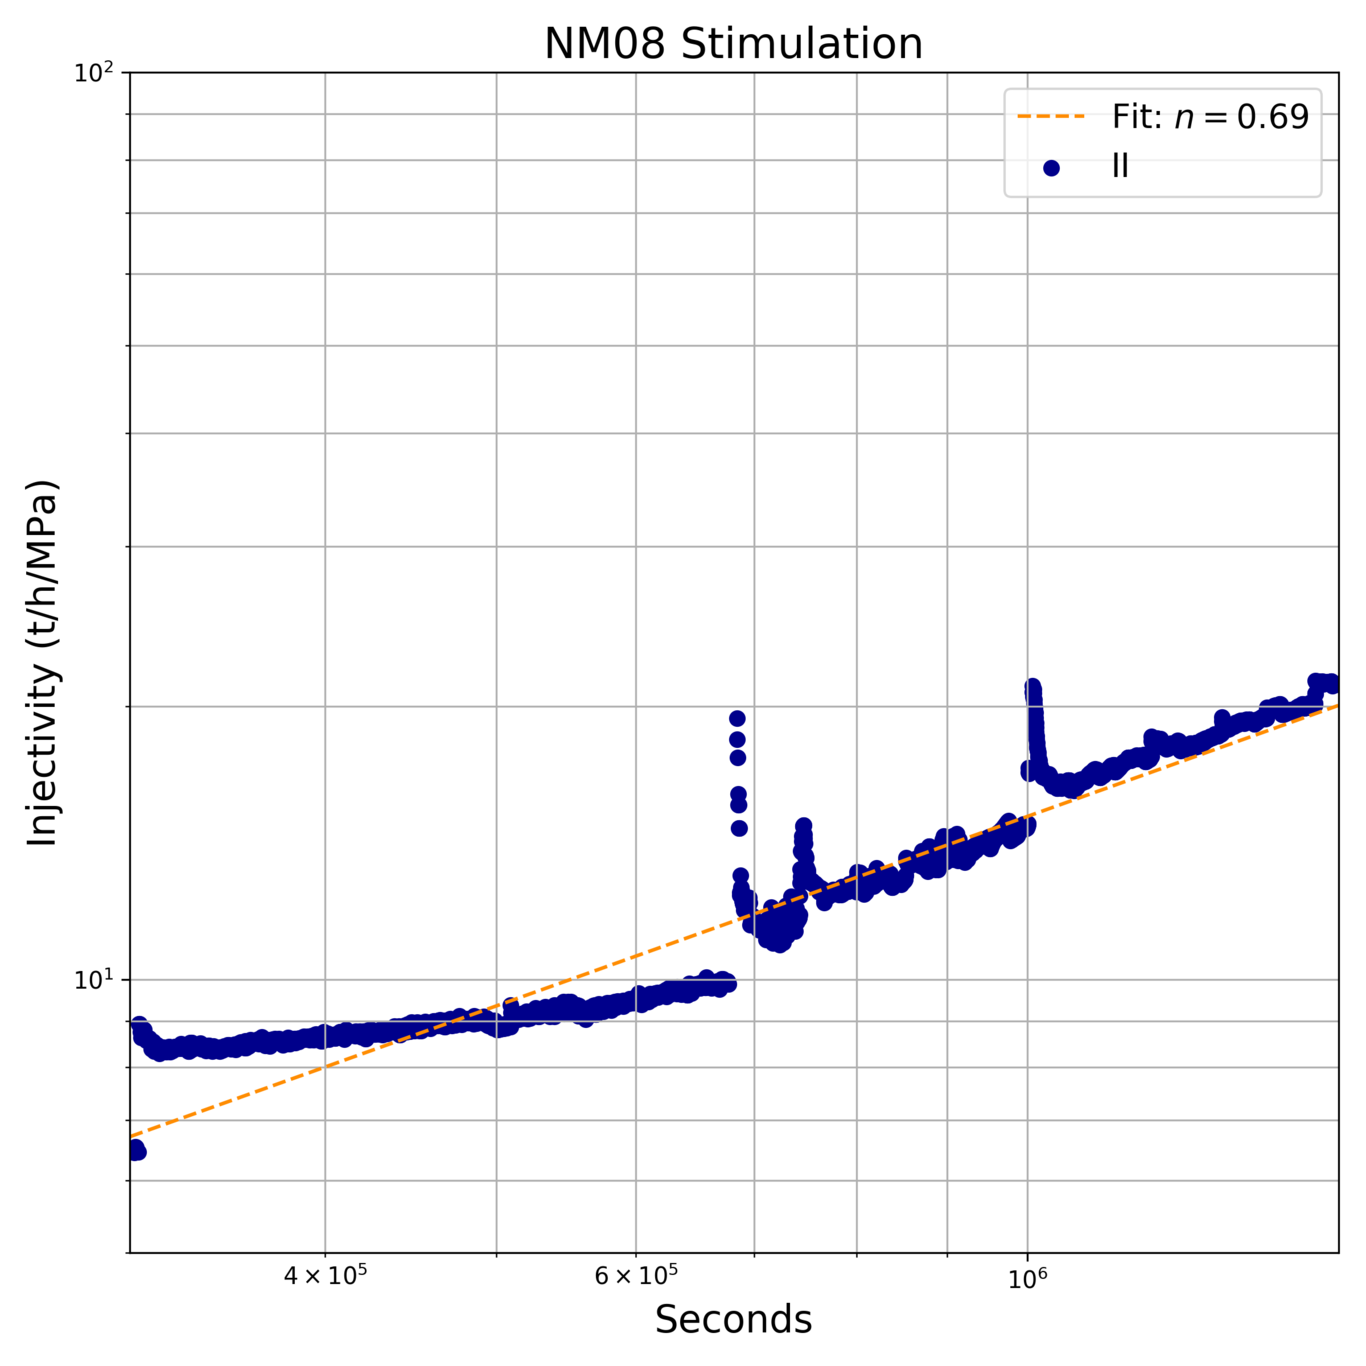
\includegraphics[width=0.70\columnwidth]{Chapter_1_Intro/figures/NM08_JC_ported_II_fitted/NM08_JC_ported_II_fitted}
\caption[Injectivity curve for NM08 stimulation]{{
\Gls{injectivity} of NM08 during a portion of the June 2012
stimulation\slash{completion} test. The rate of stimulation agrees with an
\(n\approx0.7\) relationship, which is higher than what is typically
observed at geothermal wells.
{\label{415417}}%
}}
\end{center}
\end{figure}

\Gls{permeability} is perhaps the most important property of a geothermal reservoir. It describes the ease with which fluid flows through a medium, and is the primary control on how much fluid can be taken out of, and put back into the reservoir, ultimately determining how much power can be generated \citep{Grant_2011}. As defined by Darcy's Law, \gls{permeability} is \citep{DiPippo_2016}:

\begin{equation}
k = \nu\frac{\mu{h}}{\Delta{P}}
\end{equation}

where $k$ is the reservoir \gls{permeability} (m$^2$), $\nu$ is the fluid flow velocity through the reservoir (m/s), $\mu$ is the dynamic viscosity of the fluid (Pa$\cdot$s), $h$ is the thickness of the reservoir (m) and $\Delta{P}$ is the applied pressure difference (Pa).

\Gls{transmissivity} is the \gls{permeability}-thickness product:

\begin{equation}
T = kh
\end{equation}

It describes the capacity of fluid to flow through a reservoir of thickness, $h$, and is often more convenient to work with than \gls{permeability}. This is because $kh$ is easily estimated during standard well testing operations, and because the dimensions of the reservoir (i.e. $h$) are generally unknown \citep{horne1995modern}.

Hydraulic \gls{diffusivity} is related to the \gls{permeability} by:

\begin{equation}
D = \frac{k}{\mu{s}}
\end{equation}

where $D$ is \gls{diffusivity}, $\mu$ is fluid viscosity and $s$ is the storativity of the reservoir. The diffusion of a pore fluid pressure perturbation from a well has been shown to correspond to the volume within which induced seismicity is likely to occur \citep[e.g.][]{Shapiro_2002,Parotidis_2004,Shapiro_2009,Shapiro_1997,Jeanne_2014}. This use of earthquake hypocenters to infer reservoir properties is known as seismicity-based reservoir characteriztion (SBRC) \citep{Shapiro_2002} and will be detailed in Section \ref{IS}.

\section{Geology, Development and Conceptual Models}
\subsection{Taup\={o} Volcanic Zone}
With the exception of one (Ngawha), every producing geothermal field in New Zealand is located in the central North Island. This concentration of high heat flow is known as the \acrfull{TVZ} (Figure \ref{764580}), an area of backarc extension and volcanism at the margin of the active Hikurangi Subduction Zone where the Pacific Plate subducts obliquely westward beneath the Australian Plate at a rate of $\sim$45 mm/yr \citep{Cole_1981,Wilson_1995,DeMets_1994} (Figure \ref{764580}). In the overriding plate, the rate of extension occurring along the axis of the \acrshort{TVZ} ranges from 15 mm/yr at the Bay of Plenty to \textless 5 mm/yr in the south \cite{Wallace_2004}, most of which is accommodated within the Taup\={o} Fault Belt (TFB) \cite{Villamor_2011}. Although there is currently some debate as to the extent of the \acrshort{TVZ} and how it developed \citep[e.g.][]{Stern_2011,Wilson_1995}, here we will adopt the interpretation of \citet{Wilson_2016} where the \acrshort{TVZ} is is divided into three temporal zones: the old, young and modern as well as three geographic zones: the northern, central and southern \citep{Wilson_1995,Wilson_2016}.

The evolution of the \acrshort{TVZ} began with the advent of volcanic activity at roughly 2 Ma that continues to the present day. The old \acrshort{TVZ} encompasses all identified vents and eruptive centers active during the period from $\sim$2 Ma until the emplacement of the Whakamaru Group ignimbrites (0.35 Ma), associated with the creation of the Whakamaru caldera (WH: white lines, Figure \ref{764580}) \citep{Wilson_1995}. The young \acrshort{TVZ} then includes all vents active during the period from 0.35 Ma until the Rotoiti eruption of the Okataina caldera (65ka; Figure \ref{764580}), and the modern \acrshort{TVZ} encompasses the most recent 65 ky of volcanism, with a broadly similar geometry to that of the young \acrshort{TVZ} \citep{Wilson_1995,Wilson_2016}. With the exception of the Mangakino geothermal system, the boundary of the young \acrshort{TVZ} encompasses all of the active geothermal systems in the \acrshort{TVZ} (black dotted line; Figure \ref{764580}).

The three geographic zones of the \acrshort{TVZ} are delineated based on eruptive rates, manifestation and composition. The central \acrshort{TVZ} (CTVZ) is characterized by heat flows of 700 mW/m$^2$ \citep{Bibby_1995} and \textgreater6000 km$^2$ of caldera-forming, rhyolitic volcanism \citep{Wilson_1995} (calderas, Figure \ref{764580}). The northern and southern zones (northeast of Kawerau and southwest of Tokaanu, outside the bounds of Figure \ref{764580}) are characterized by andesite-dacite composite cones (larger in the south) and very little rhyolitic or basaltic products. The eruptive rate in the south is less than one third and the heat flow one fifth of that in the central \acrshort{TVZ} \citep{Wilson_2016}. These values are poorly constrained in the north, mostly due to its subaqueous nature, but the output is likely even less than that in the south \citep{Wilson_2016}.

The CTVZ, where all of the active \acrshort{TVZ} geothermal systems are located, is made up of at least eight separate, rhyolite calderas, of which the two most recently active are Taup\={o} in the southwest and Okataina in the northeast \citep{Wilson_1995}. The Ngatamariki and Rotokawa systems both lie at the eastern edge of the 0.35 Ma Whakamaru caldera and within the Taup\={o}-Reporoa Basin (TRB) \citep{Wilson_2016,Downs_2014} (Figure \ref{764580}). Heat flow within the TRB is the highest in the \acrshort{TVZ}, as evidenced by the concentration of geothermal systems \citep{Wilson_2016}. However, the TRB is sparsely faulted relative to the Taup\={o} Fault Belt to the west, where most of the active extension is accommodated (indicated by the high concentration of faults in Figure \ref{764580}). The reasons for this discrepancy are poorly understood and the interactions between modern tectonics, inherited structures (i.e. caldera rims and basement faults), magmatism and heatflow will need to be unraveled before sense can be made of the locations of the CTVZ geothermal systems.\selectlanguage{english}

\begin{figure}[h!]
\begin{center}
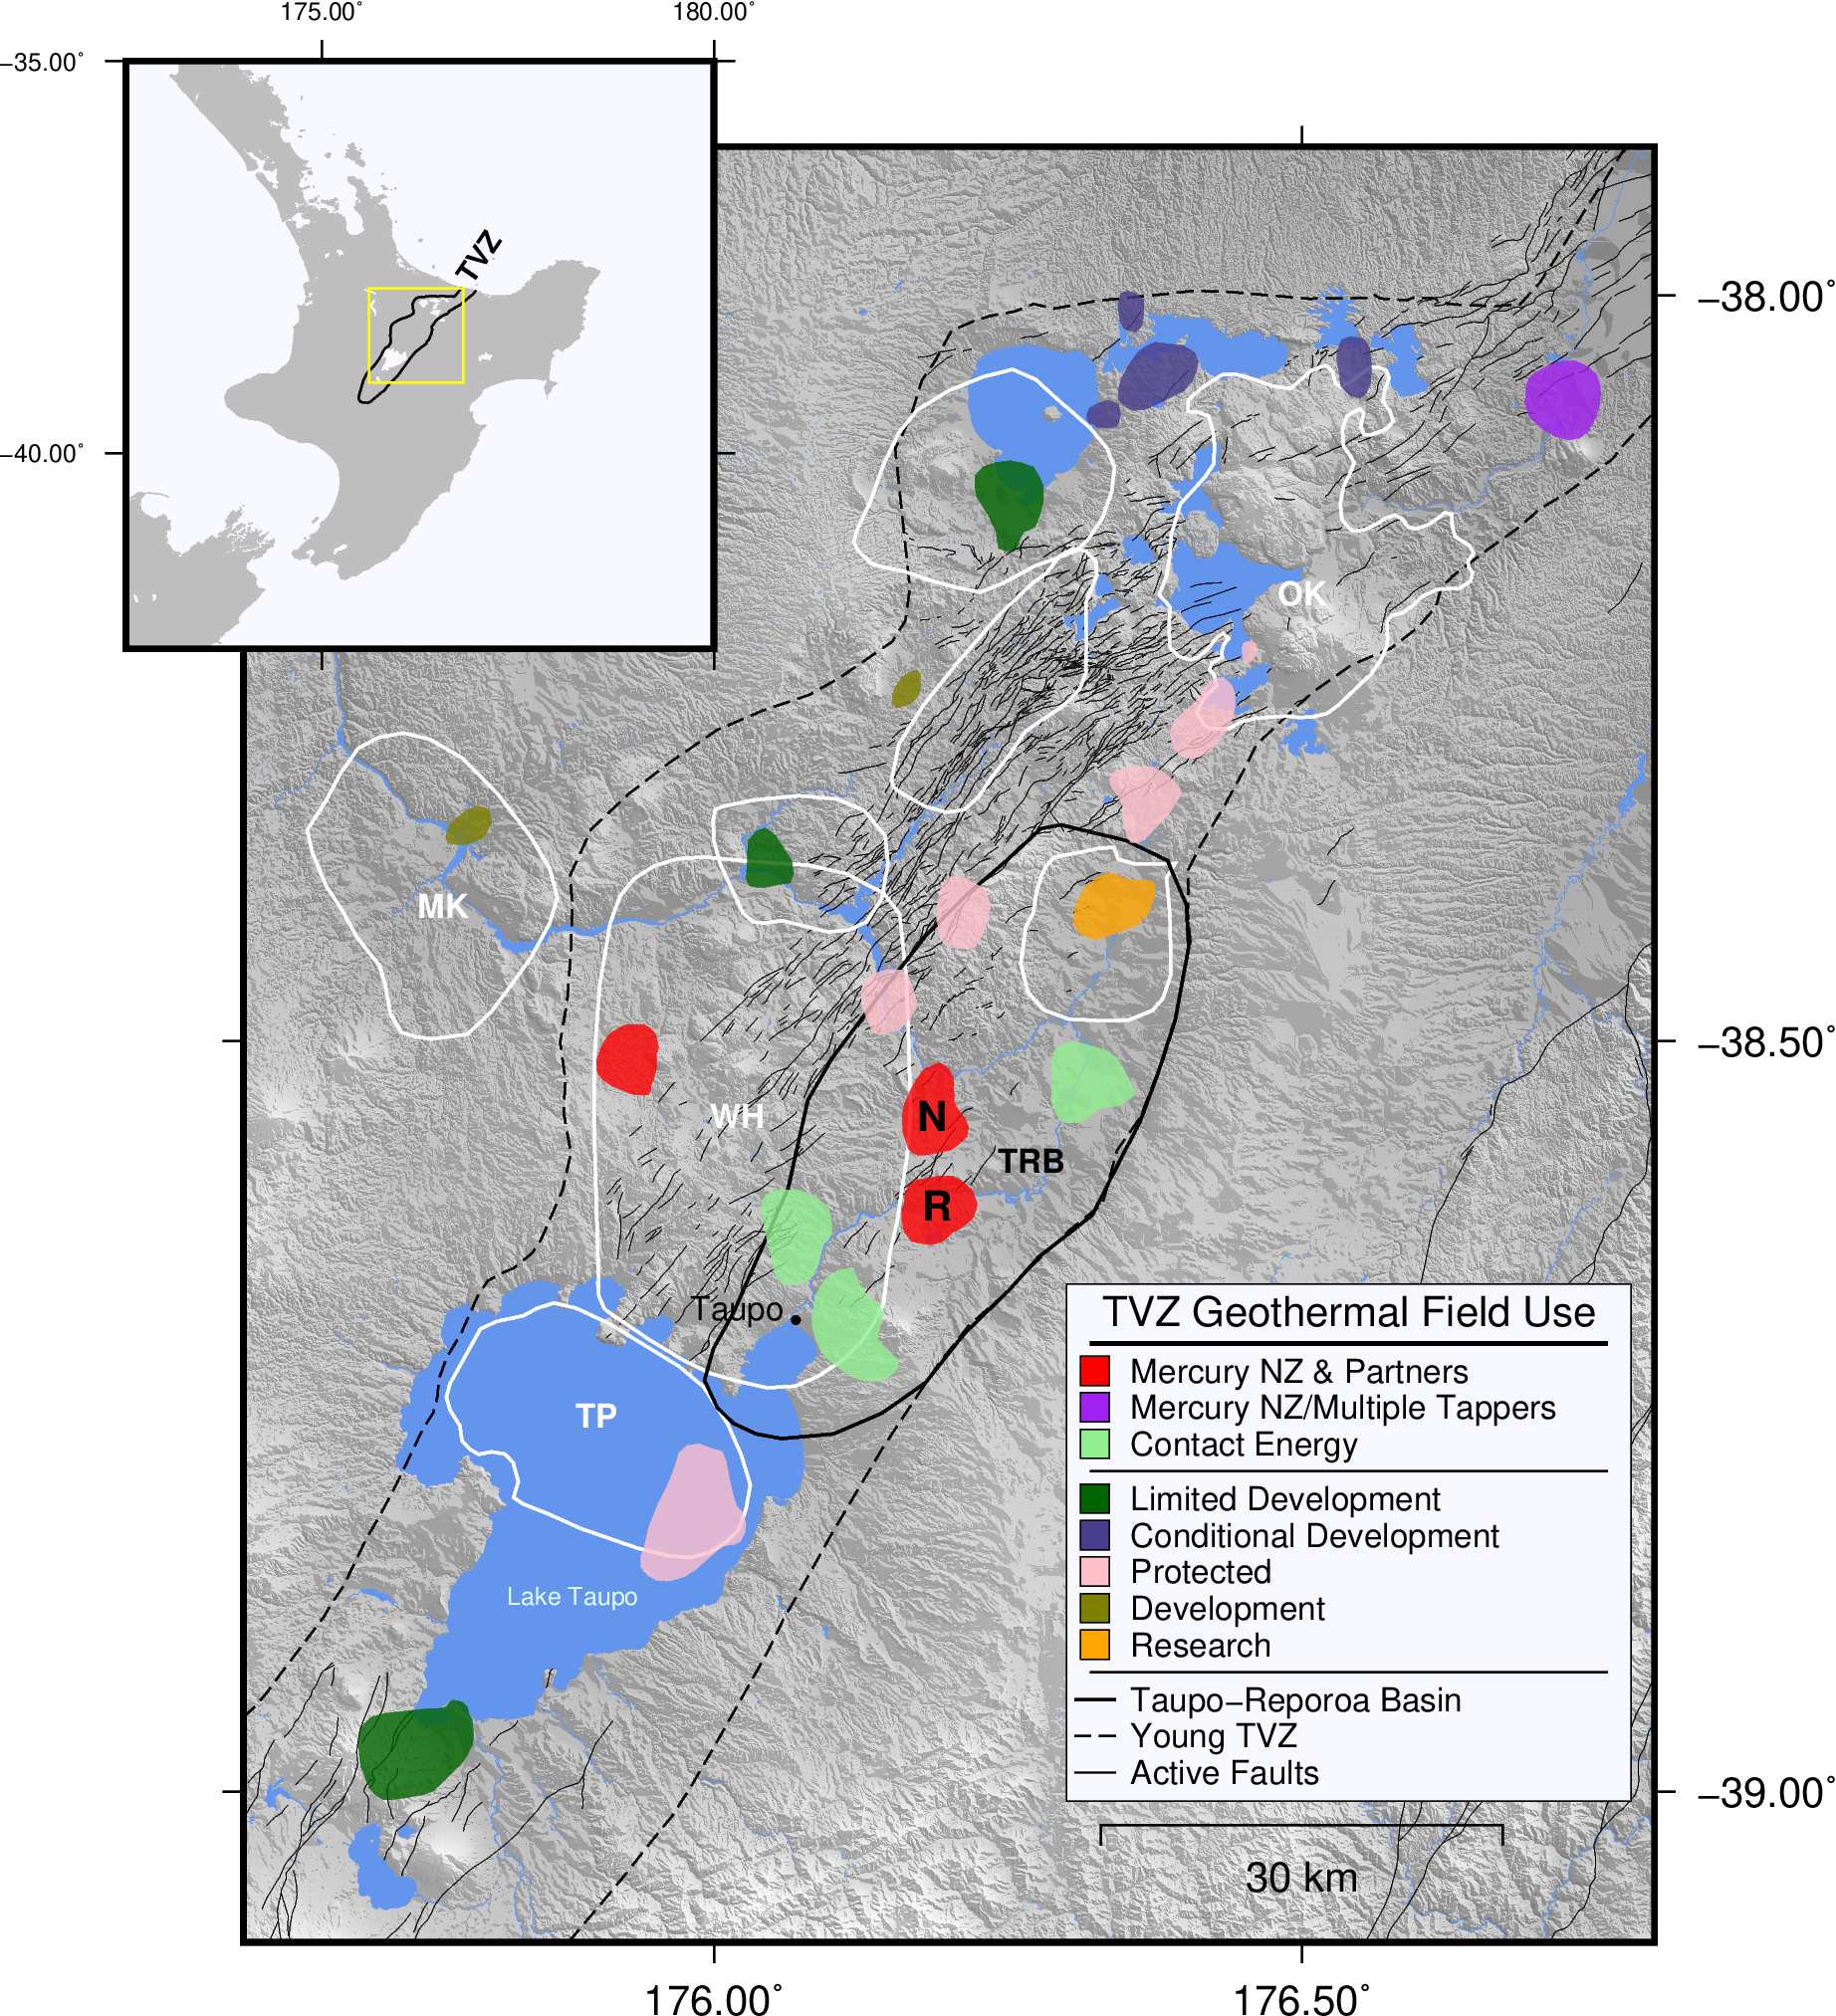
\includegraphics[width=1.00\columnwidth]{Chapter_1_Intro/figures/Geothermal_fields_TVZ_w_usage/TVZ_geothermal_overview_large}
\caption[Location of the geothermal fields in the \acrshort{TVZ}]{{
The resistivity boundaries of the 23 geothermal fields in the Central
Taup\={o} Volcanic Zone (CTVZ) (after \protect\citet{Bibby_1995}) colored by degree
of development or geothermal operator. Rotokawa and Ngatamariki are
labeled `R' and `N', respectively. The boundary of the young \acrshort{TVZ}, as
defined by~\protect\citet{Wilson_1995} ,~ is shown as a dotted line and their
eight identified rhyolitic calderas are outlined in white (Whakamaru
Caldera: `WH', Taup\={o} Caldera: `TP', Okataina: 'OK', Mangakino: 'MK'). The Taup\={o}-Reporoa
Basin (TRB) is outlined in thick black after~\protect\citet{Downs_2014}.~~
{\label{764580}}%
}}
\end{center}
\end{figure}

\subsection{Ngatamariki}
\subsubsection{Geology}
The Ngatamariki geothermal field is located approximately 17 km north of the town of Taup\={o} (Figures  \ref{764580}, \ref{425195}). Ngatamariki is a high-temperature, liquid-dominated and naturally-fractured system (up to 280\textdegree{}C at depths exceeding 1000 m) that measures roughly 5.5 km from north to south and 3 km east to west \citep{Bignall_2009, Chambefort_2014}. The reservoir is hosted in volcanic rocks of pre-Whakamaru age, known as the Reporoa Group (old \acrshort{TVZ}, \textgreater0.35 Ma)\citep{Chambefort_2014}. In the southern portion of the field, the earliest unit in the Repora Group is the Rotokawa Andesite, which overlies the Torlesse Greywacke basement and, therefore, represents the onset of volcanism in the \acrshort{TVZ} \citep{Chambefort_2014,Wilson_2016} (Figure \ref{673646}). The overlying units are referred to as the Tahorakuri Formation and consist of older andesitic lava flows and younger volcaniclastic units of varying composition, accounting for $\sim$1 Ma of volcanism \citep{Chambefort_2014}. In the northern part of the field, the upper Tahorakuri volcanic sequence is overlain by a sedimentary succession that is interpreted to represent a period of relative volcanic quiescence and active tectonism \citep{Chambefort_2014}. At that time, the Ngatamariki intrusive complex was emplaced in the northern part of the field, the only such plutonic body yet sampled in the \acrshort{TVZ} \citep{Chambefort_2014}. This $\sim$0.7 Ma tonalite-diorite body defines the deeper portion (\textgreater2000 m bsl) of the northern reservoir, where in the south the Rotokawa Andesite is found \citep{Chambefort_2014} (Figure \ref{673646}). Overlying the Tahorakuri across most of the field is the Whakamaru Group ignimbrite, associated with the creation of the Whakamaru Caldera (WH, Figure \ref{764580}) and start of young \acrshort{TVZ} volcanism \citep{Chambefort_2014,Wilson_1995}. The younger overlying units represent various periods of volcanism and sedimentation through to the deposition of the modern surface deposits \citep{Chambefort_2014} (Figure \ref{673646}).

There are a number of mapped (Figure \ref{425195}) and buried (Figure \ref{673646}) normal faults within the Ngatamariki reservoir, defining small horst-and-grabben structures at depth \citep{Bignall_2009}. In the south, the larger of these structures are related to the active NE-SW Aratiatia Fault Zone (Figure \ref{425195}), while in the northern reservoir, faulting is less extensive at the surface \citep{AFDB}. The primary structural trend in the field is NE-SW, related to the current extensional tectonic regime, with a subordinate NNW-SSE trend that has been attributed to the fabric of the Whakamaru caldera margin \citep{Bignall_2009}. This trend extends from the scale of mapped faults down to centimeter-scale fractures as interpreted from borehole image logs in both the northern and southern parts of the field \citep{nm09_report,nm10_report,massiot_2012}.\selectlanguage{english}

\begin{figure}[h!]
\begin{center}
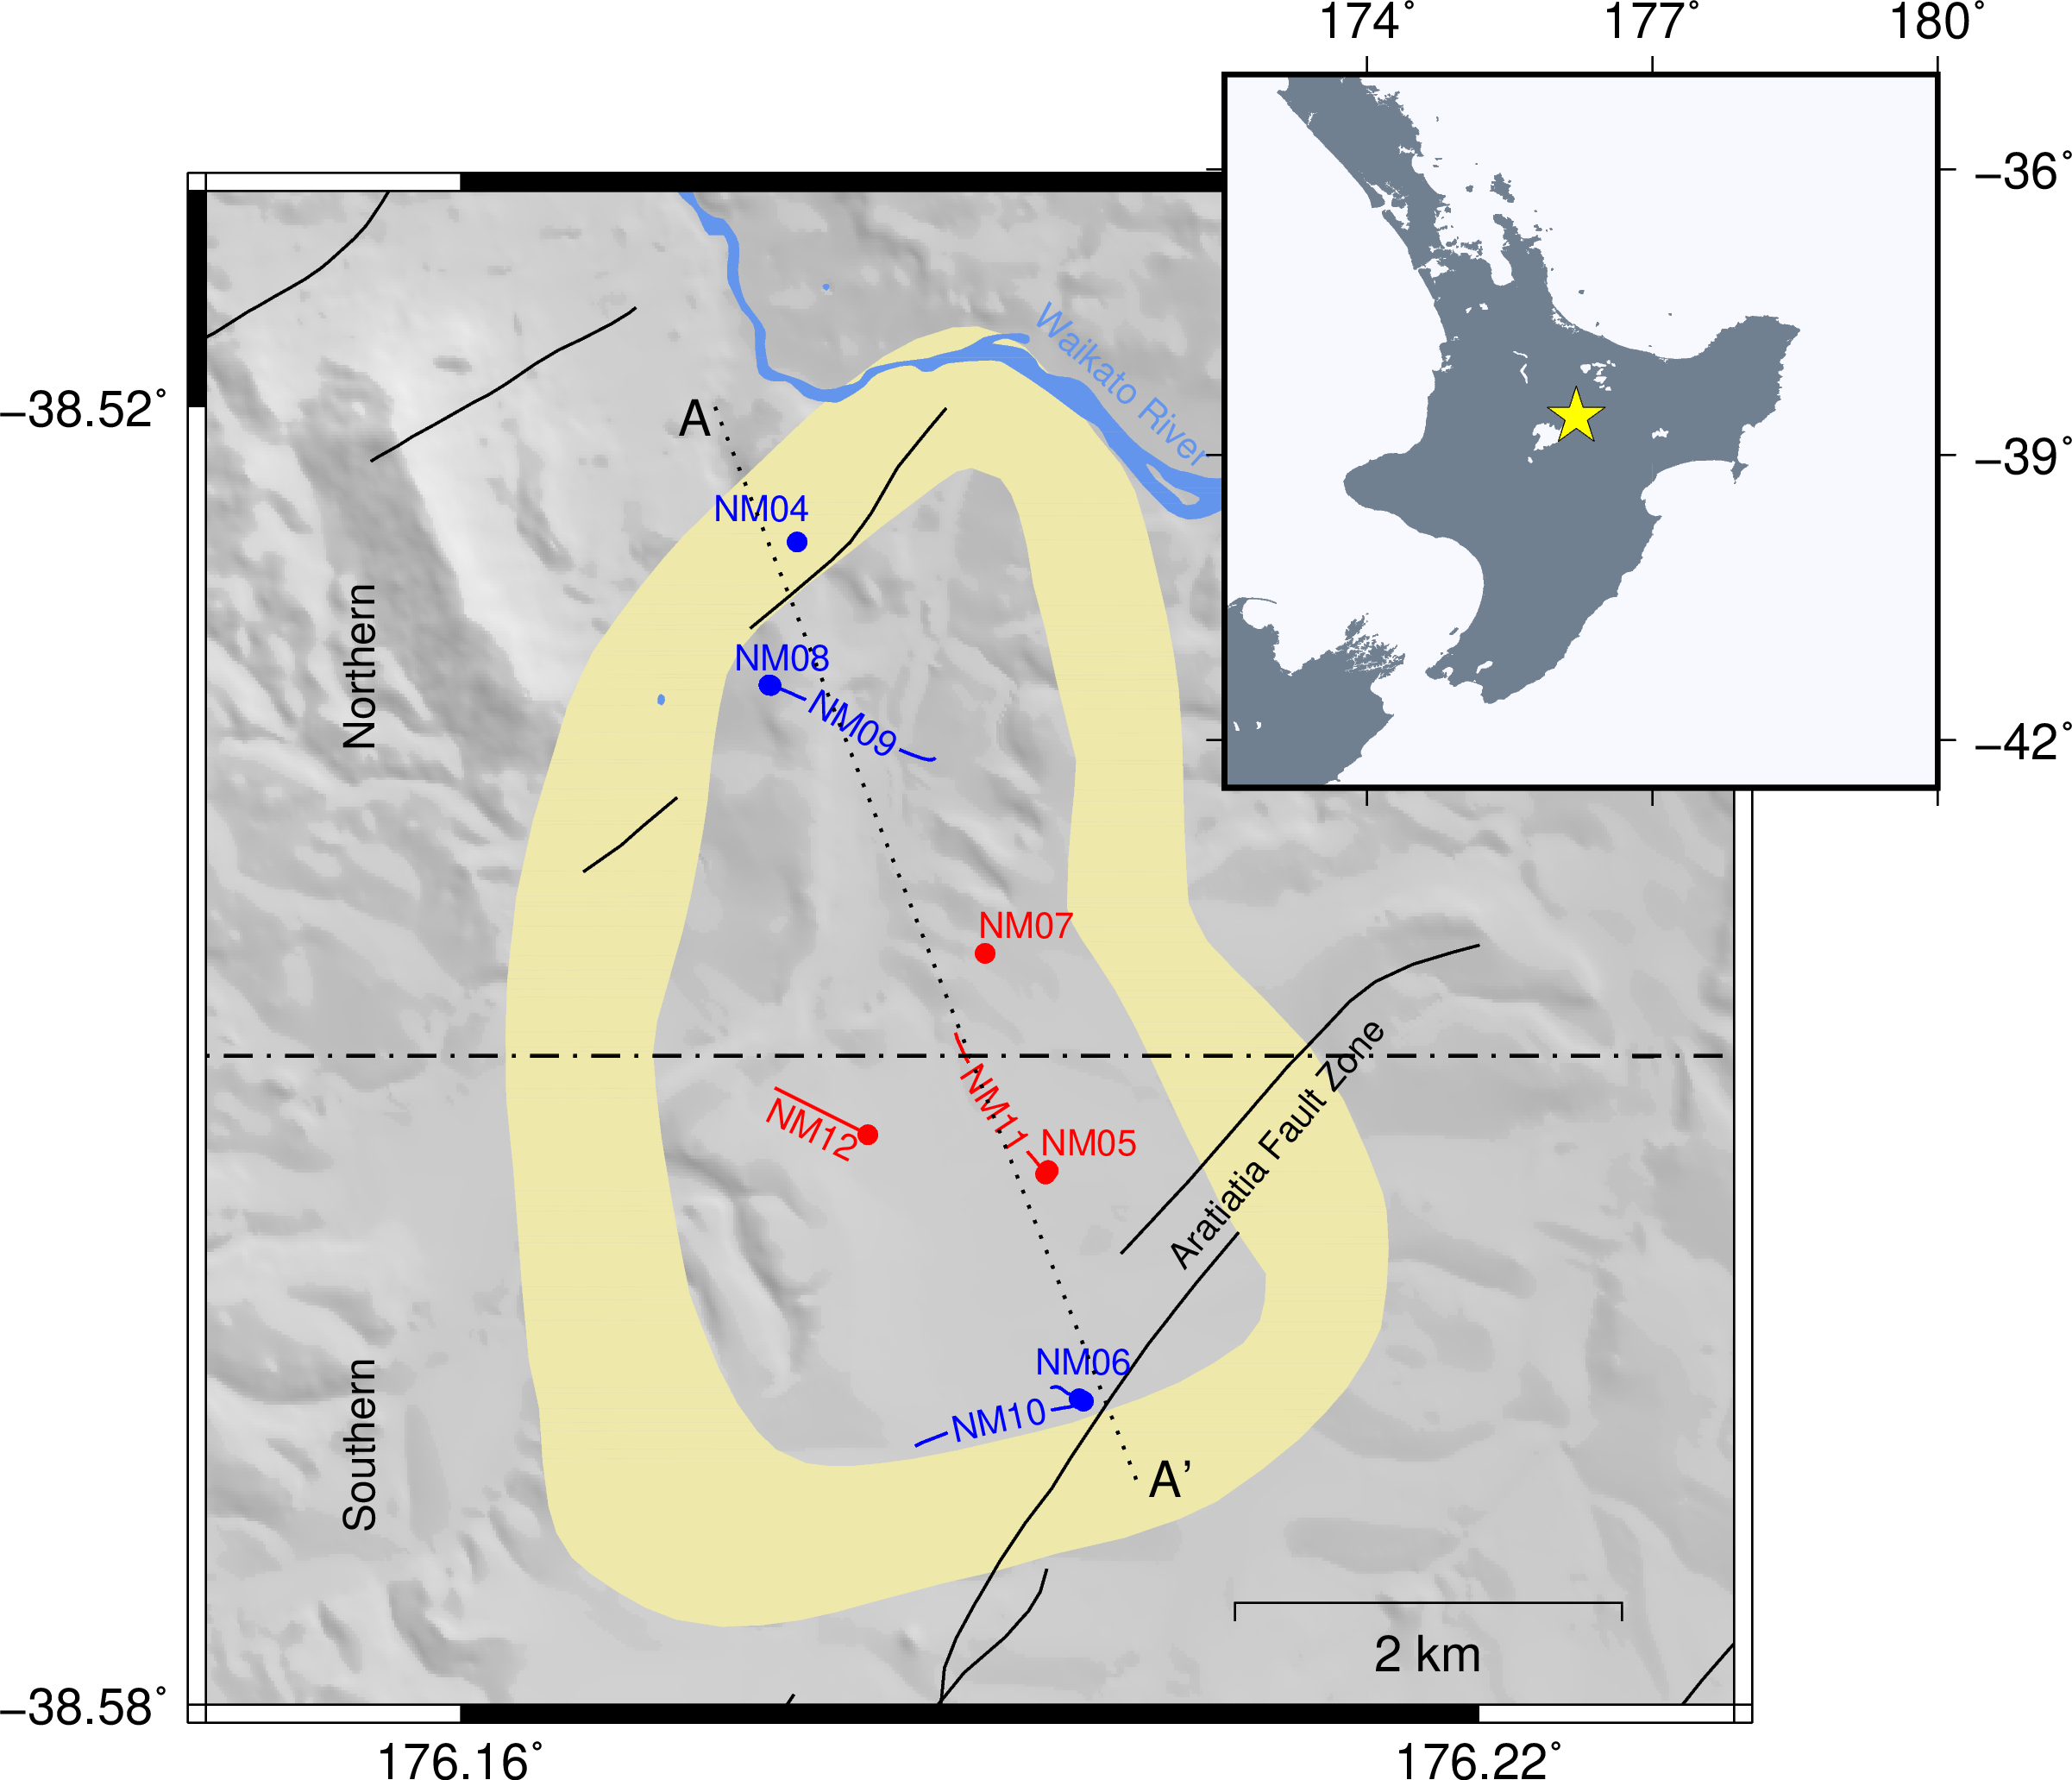
\includegraphics[width=0.70\columnwidth]{Chapter_1_Intro/figures/merc_Nga_overview_temps-wells_12-15_no_inset/merc_Nga_overview_wells_12-15}
\caption[Overview of the Ngatamariki geothermal field]{{
Overview of the Ngatamariki geothermal field. Injection wells are shown
in blue, production wells in red with dots representing the wellhead and
lines showing the surface projection of the well at depth. Wells NM04,
NM08, NM05 and NM07 are near vertical and, therefore, appear only as
dots in the figure.~ Active faults from the GNS Active Faults
Database \citep{AFDB} are shown in black. The most likely boundary
of the deep resource as published by~\protect\citet{Boseley_2010} based on
magnetotelluric surveys, is shown in yellow. The surface projection of the cross-section corresponding to Figures \ref{673646} and \ref{813462} is dotted line A--A`. The location of the field on the North Island is shown as a star on the inset map.
{\label{425195}}%
}}
\end{center}
\end{figure}\selectlanguage{english}

\begin{sidewaysfigure}[p]
\begin{center}
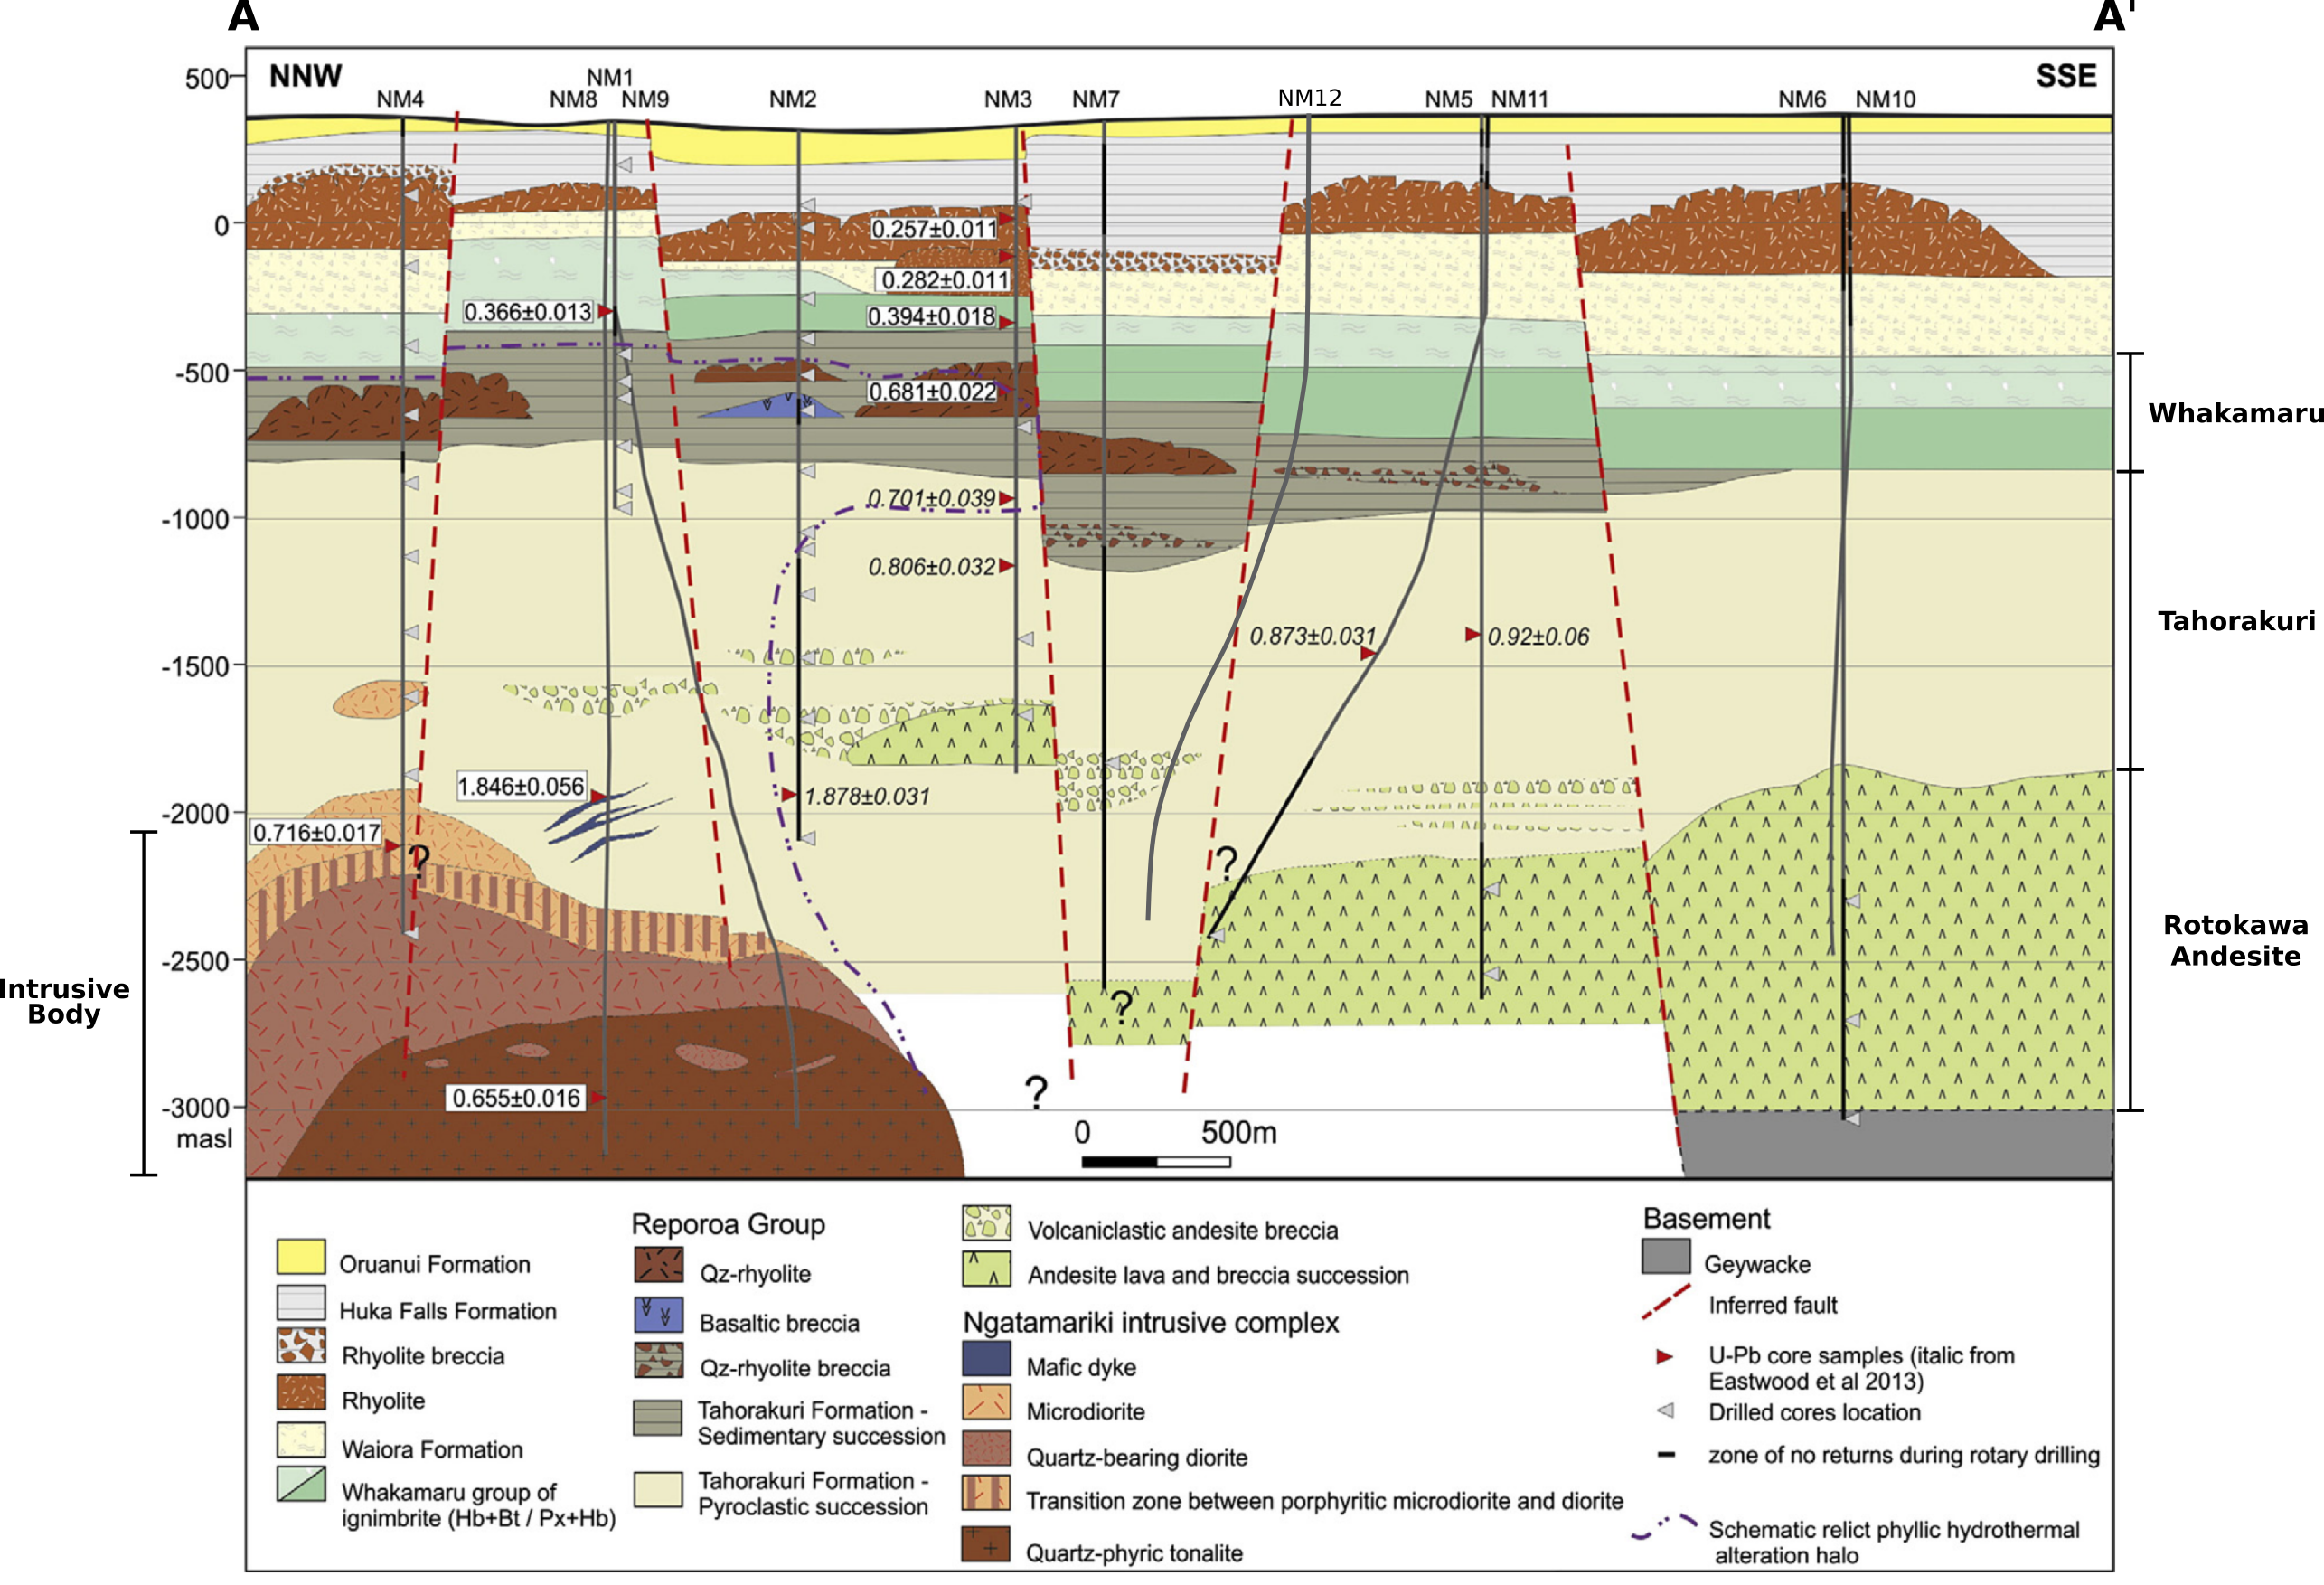
\includegraphics[width=0.7\textwidth,height=\textheight,keepaspectratio]{Chapter_1_Intro/figures/Chamberfort_2014_fig3/Chamberfort_2014_fig3_mod_lores}
\caption[Detailed cross-section of Ngatamariki geology]{{
Detailed geologic and structural context for the Ngatamariki geothermal
field from~\protect\citet{Chambefort_2014} including U-Pb dates (red triangles and
black text) and locations of core from each well. Question marks
correspond to contacts or faults that are consistent with borehole data, but which are not confirmed. The surface trace of the cross-section is shown in Figure \ref{425195}.
{\label{673646}}%
}}
\end{center}
\end{sidewaysfigure}

\subsubsection{Development}
Development at Ngatamariki began with the drilling of four deep exploration wells by the New Zealand government in 1984 \citep{Clearwater_2015}. Although these demonstrated the existence of a potentially viable resource, full-scale development for geothermal power was not undertaken until 2004 when Mercury (then known as Mighty River Power) partnered with the Tauhara No. 2 Trust, representing the local Maori landowners, to drill additional wells and eventually build the current, 82 \acrshort{MWe} power station \citep{Clearwater_2015}. Between June 2012 and February 2013, NM08, NM09 and NM10 were drilled as injection wells at the periphery of the deep reservoir. For each, a completion\slash{stimulation} test was conducted \citep{Clearwater_2015}. The Ngatamariki power plant was then brought online starting in April 2013 with gradually increasing \glspl{flow_rate} until the reservoir reached a roughly stable state at around the start of 2015 (Figure \ref{953396}).

Mercury have identified three periods between 2012 and 2015 during which the relationship between injection and production parameters and seismicity is of particular interest. We have added the period of NM08 stimulation that was previously analyzed by \citet{matson2019thesis}:
\begin{itemize}
  \item{NM08 Stimulation}
  
  From June 7 until July 10, 2012 (Figure \ref{953396}), northern injection well NM08 (Figure \ref{425195}) underwent a completion and stimulation test. Although low \gls{permeability} was encountered during drilling, NM08 responded well to stimulation \citep{Clearwater_2015}. MSc student Gabe Matson analyzed this particular injection using similar techniques to what will be detailed in this work \citep{matson2019thesis}. Here, we also analyze this period and compare our results to those obtained independently by \citet{matson2019thesis} to check our methodology.
  \item{NM09 Stimulation}
  
  From December 2012 until late January 2013 (Figure \ref{953396}), northern injection well NM09 (Figure \ref{425195}) also underwent completion and stimulation testing. NM09 responded positively to stimulation, although not as positively as NM08 and very little seismicity was detected \citep{Clearwater_2015}.
  \item{NM10 Drilling Losses and Stimulation}
  
  In July 2012 (Figure \ref{953396}), total fluid losses were encountered during drilling of southern injection well NM10 (Figure \ref{425195}). This was followed a month later by a completion and stimulation test, as at NM08 and NM09.
  \item{NM12 Drilling Losses}
  
  Similar to what occurred at NM10 in 2012, total fluid losses were incurred during the drilling of production well NM12 from June to September 2014 (Figure \ref{953396}).
\end{itemize}

In addition to these periods of interest, we will also investigate the seismic response to the plant startup at Ngatamariki (Figure \ref{953396}), which involved flow rates up to five-times greater than during the periods outlined above, and \acrshort{WHP} of up to 2.0 MPa.\selectlanguage{english}

\begin{figure}[h!]
\begin{center}
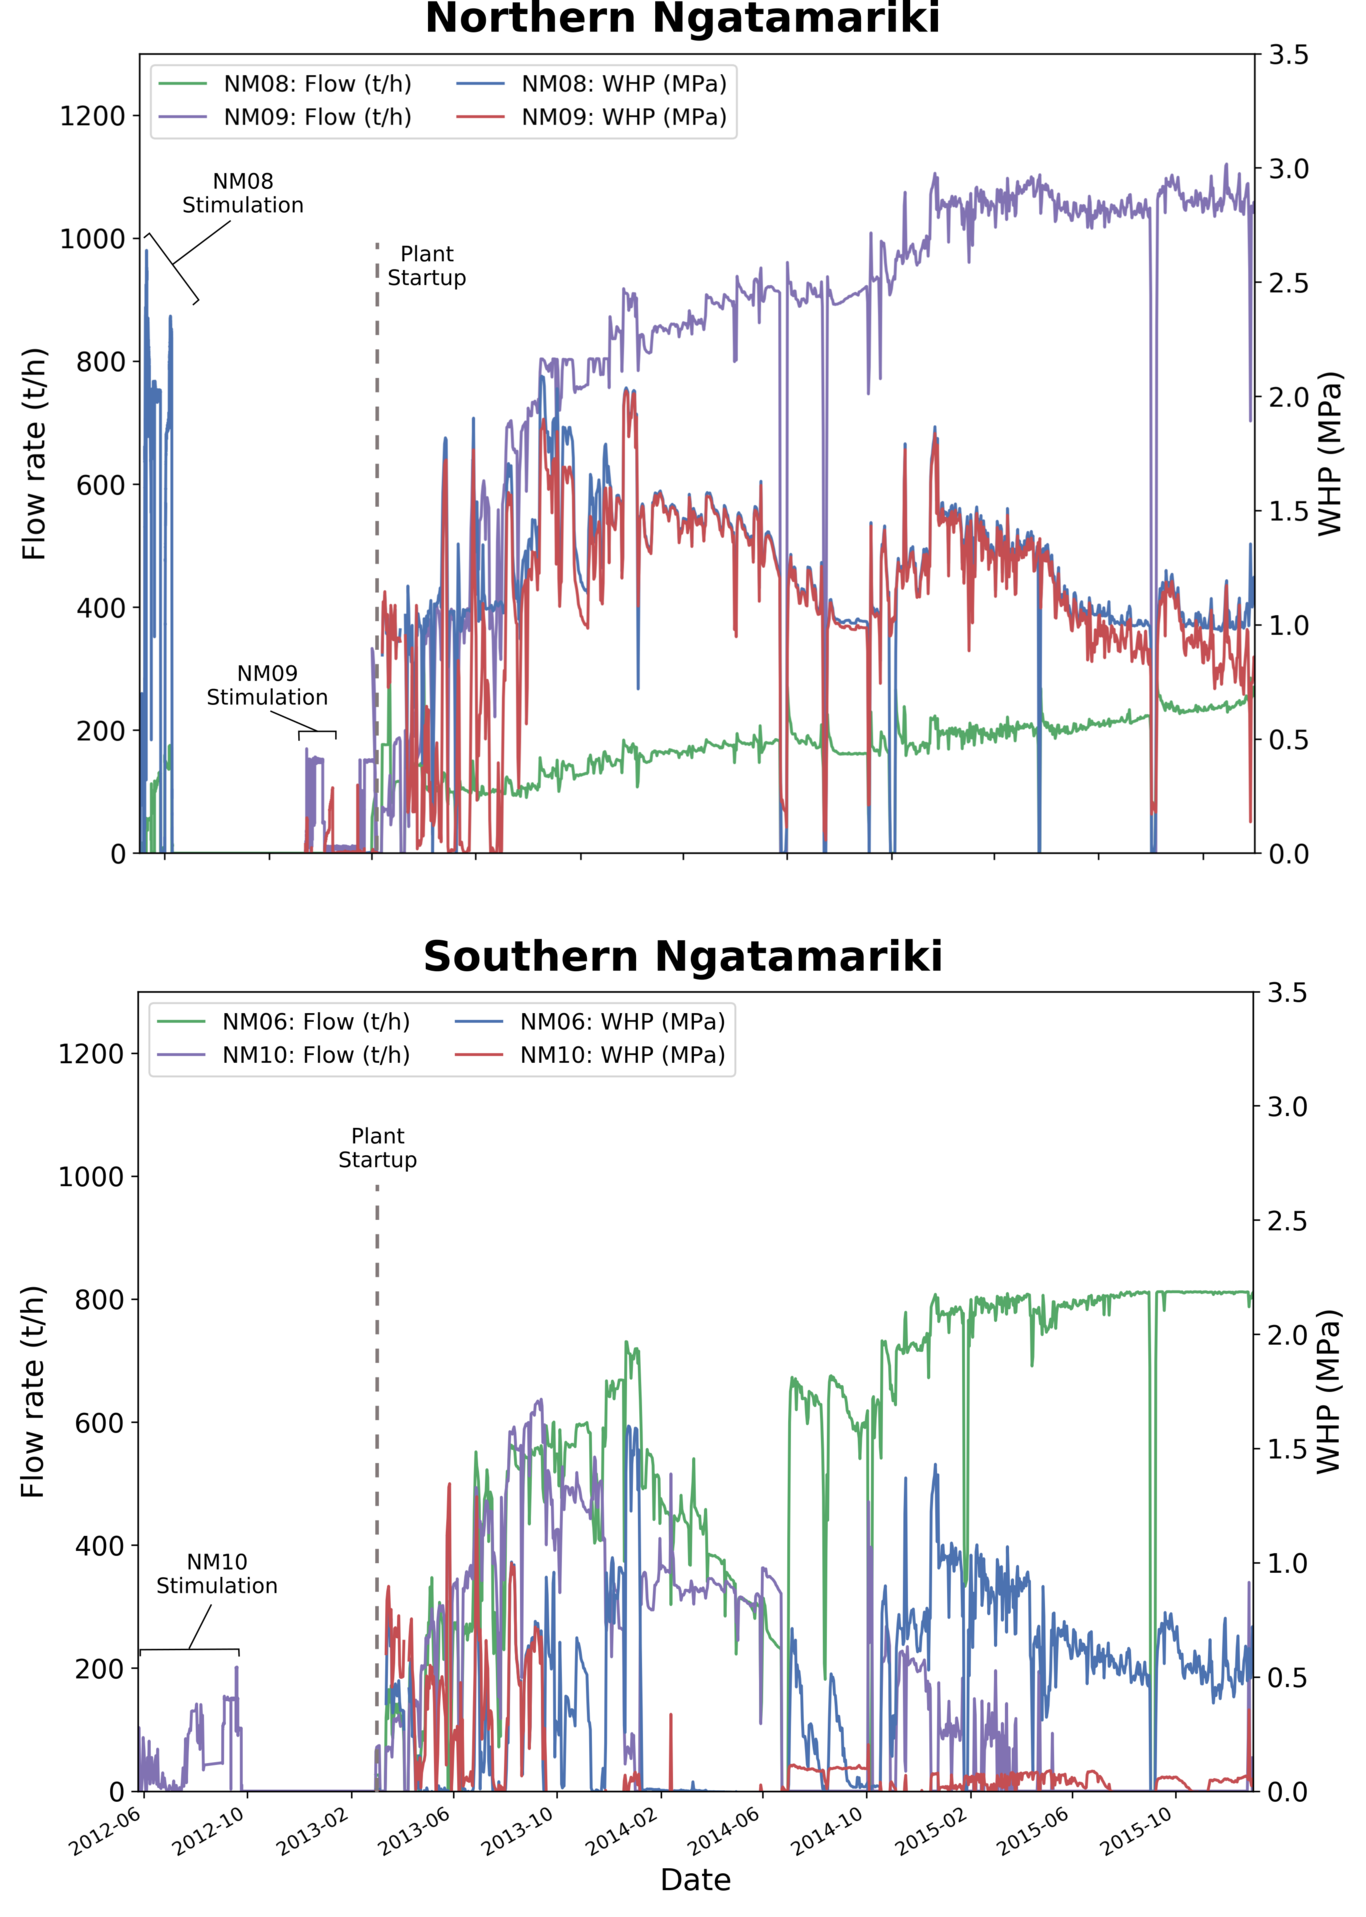
\includegraphics[width=0.84\columnwidth]{Chapter_1_Intro/figures/NgaN_ALL_flows_WHP/Ngatamariki_overview_Intro}
\caption[Flow rates and \glspl{WHP_g} at Ngatamariki: 2012--2015]{{
Summary figure including the \glspl{flow_rate} and \glspl{WHP_g} at each
of the four injection wells at Ngatamariki for 2012-2015 (separated into
northern and southern injection zones). The main periods of interest,
including the three completion\slash{stimulation} tests and the plant startup
are annotated. Drilling of NM12 occurred between June and September 2014, but is not annotated here as we have no flow data for that operation.
{\label{953396}}%
}}
\end{center}
\end{figure}

\subsubsection{Conceptual Model}
Hydrologically, Ngatamariki consists of three semi-isolated aquifers at differing depths: the shallow aquifer at the surface, an intermediate aquifer above $\sim$500 m bsl, and the deep geothermal reservoir below that \citep{Boseley_2010,Chambefort_2016} (Figure \ref{813462}). Each of these aquifers is separated by an impermeable layer that, for silicic volcanic rocks in the presence of acidic fluids, is created by alteration to illite-smectite clay \citep{Boseley_2010}. These layers are normally diagnostic of geothermal reservoirs and are generally inferred from areas of low resistivity \citep[e.g.][]{Bibby_1995} and conductive intervals of well temperature profiles \citep{Grant_2011}. The deep reservoir at Ngatamariki is isolated from the intermediate aquifer by a clay cap that ranges in thickness from \textgreater1000 m at the northern periphery to practically nonexistent between monitoring\slash{exploration} wells NM2 and NM3, where \citet{Boseley_2010} have inferred a hydrologic connection to the intermediate aquifer called `the leak' (Figure \ref{813462}). This point also marks the center of the `upflow', which refers to the area of upward convection within a geothermal system and is commonly a target for production wells \citep{Grant_2011}. Reservoir \gls{permeability} in the \acrshort{TVZ} is dominated by existing faults and fractures, as the matrix \gls{permeability} of the major formations is low \citep{Grant_2011,Cant_2018}. This is certainly the case at Ngatamariki, where the Tahorakuri Formation and Rotokawa Andesite that host the reservoir are shown to be highly fractured in image logs \citep{nm09_report,nm10_report,massiot_2012} and fracture-dominated flow is assumed by reservoir modelers \citep[e.g.][]{Quinao_2018}.\selectlanguage{english}

\begin{sidewaysfigure}[p]
\begin{center}
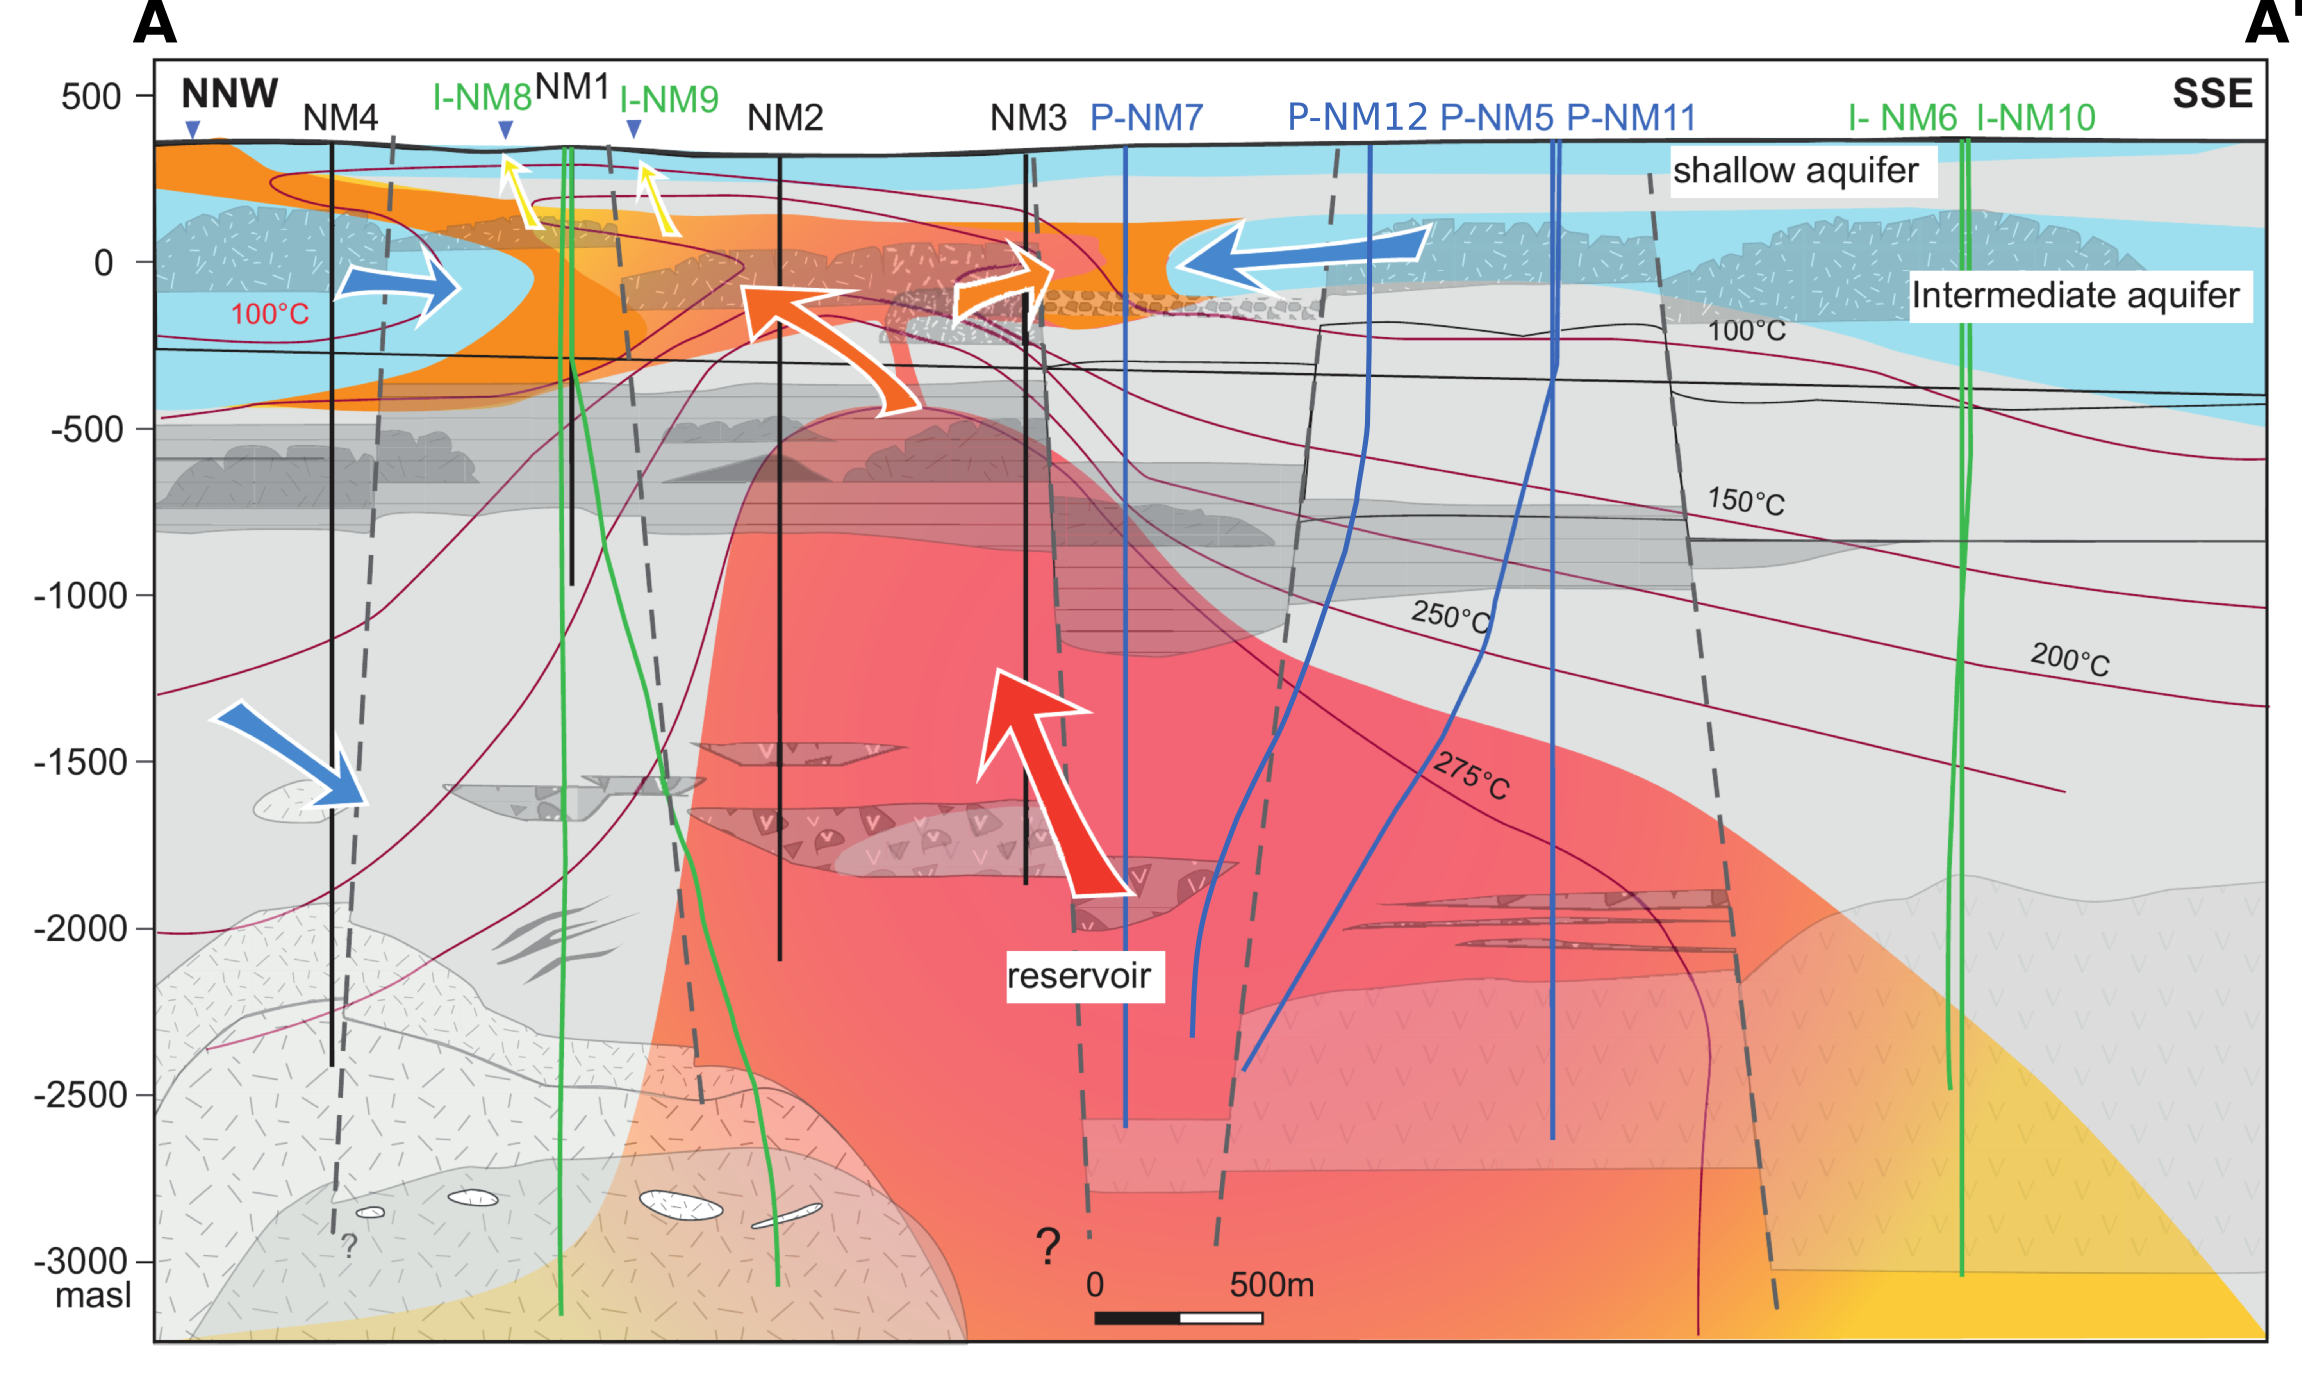
\includegraphics[width=0.7\textwidth,height=0.7\textheight,keepaspectratio]{Chapter_1_Intro/figures/Chamerfort_2015_fig9_model/Chambefort_2015_fig9_model_lores}
\caption[Cross-section of the Ngatamariki conceptual model]{{
Ngatamariki conceptual model proposed by~\protect\citet{Boseley_2010} overlain on
the geologic cross-section in Figure~{\ref{673646}}
by~\protect\citet{Chambefort_2016}. In this figure, green wells are injection wells
and blue are production. Note that, for most figures in this work, blue
wells will signify injection and red production. The main upflow at
Ngatamariki is located between wells NM2 and NM3, in the northern part
of the reservoir. Arrows indicate flow direction with the color
signifying the relative temperature of the fluid (red=hot, blue=cold).
Maroon lines are isotherms modeled from well temperature profiles.
{\label{813462}}%
}}
\end{center}
\end{sidewaysfigure}

Nearly all of the produced fluid at Ngatamariki is reinjected into the reservoir. In order to maintain flexibility with regard to reservoir management, there are two reinjection fields (green wells, Figures \ref{425195}, \ref{813462}, blue lines in all other figures) to the north and south of the central production field (blue lines, Figure \ref{813462}, red lines in all other figures). The distribution of injection between the two fields varies with time in response to changes in the reservoir and borehole degradation. Generally, more fluid is injected into the northern injection zone than the southern. NM09, in the north, is the dominant injection well for the entire field (currently \textgreater1000 t/h). However, \gls{permeability} heterogeneity is considerable. Well NM08 is far less permeable than NM09, although they are separated by only hundreds of meters at reservoir depth \citep{Clearwater_2015}. Permeability also varies substantially with depth, particularly in the northern injection zone where the wells intersect the diorite\slash{tonalite} intrusive body, which has a very low matrix \gls{permeability} \citep{Cant_2018}.

While all of the wells drilled at Ngatamariki can be considered to be highly-fractured \citep{nm09_report,nm10_report,massiot_2012}, only a portion of these fractures are open and able to accept fluid upon injection or production (we refer to these high-\gls{permeability} areas as \glspl{feedzone}). Therefore, the most permeable wells in the field are those that intersect active fracture zones that have a high likelihood of being open and not filled with minerals. Such high-\gls{permeability} fracture zones are intersected at NM09, NM06 and NM10, but not at NM08 \citep{nm09_report,nm10_report,massiot_2012}.

In the southern injection zone, radioactive \glspl{tracer_test} have revealed well NM10 to be well-connected, hydrologically, to the southern production well NM5 \citep{buscarlet_2015}. As such a connection produces a loss in entropy (cooler water is extracted), and therefore a loss in power generation capacity at the plant, injection at NM10 was phased out by early 2015 (Figure \ref{953396}). The excess injection in the southern part of the field was then accommodated by NM06 (Figure \ref{425195}).

\subsection{Rotokawa}
\subsubsection{Geology}
The Rotokawa geothermal field is located $\sim$7 km south of Ngatamariki. As defined by the resistivity boundaries shown in Figure \ref{838185} \citep{Risk_2000}, the resource measures approximately 4 km in diameter. The surface projection of the resource sits astride the Waikato River and all of the development to-date has occurred south of the river. Rotokawa is also a naturally-fractured, liquid-dominated reservoir, but the maximum temperatures encountered at depth are the highest measured in the \acrshort{TVZ} (338\textdegree C in well RK22). Given their close proximity, the geology at Rotokawa is very similar to that of Ngatamariki, although the heterogeneity of the young \acrshort{TVZ} volcanic deposits and active faulting have led to certain differences. Most importantly, while the Ngatamariki reservoir is hosted in Rotokawa Andesite and Tahorakuri Formation rocks, the shallower depth to the basement at Rotokawa (up to 1700 m bsl) means that much of the reservoir is hosted in Torlesse Greywacke (Figure \ref{599670}) \citep{wallis2013,McNamara_2016}. The rest of the Rotokawa reservoir is mostly hosted in Rotokawa Andesite which reaches thicknesses of 1500 m and is laterally coherent across the field, although the shallower parts of the production field (red wells, Figure \ref{838185}) are hosted in varying thicknesses of Tahorakuri Formation and Wairakei Ignimbrite (part of the Whakamaru Group; \textless0.35 Ma age) \citep{McNamara_2016}. At Rotokawa, there is no analog to the intrusive complex intersected in wells NM04, NM08 and NM09 at Ngatamariki.

The regional NE-SW structural grain describes the first-order structure at Rotokawa, with the Aratiatia Fault Zone cutting across the northwest corner of the field (Figure \ref{838185}) and three NE-SW-striking faults dividing the reservoir at depth: the \acrfull{PFF}, \acrfull{CFF} and \acrfull{IFF} (Figure \ref{599670}) \citep{wallis2013}. Each of these faults is inferred from vertical offsets in the basement greywacke and Rotokawa Andesite observed from well cuttings, microseismic locations and radioactive tracer returns between wells \citep{Sewell_2015,Addison_2017stanford,wallis2013}, but they are not observed to offset the overlying units \citep{wallis2013}.\selectlanguage{english}

\begin{figure}[p]
\begin{center}
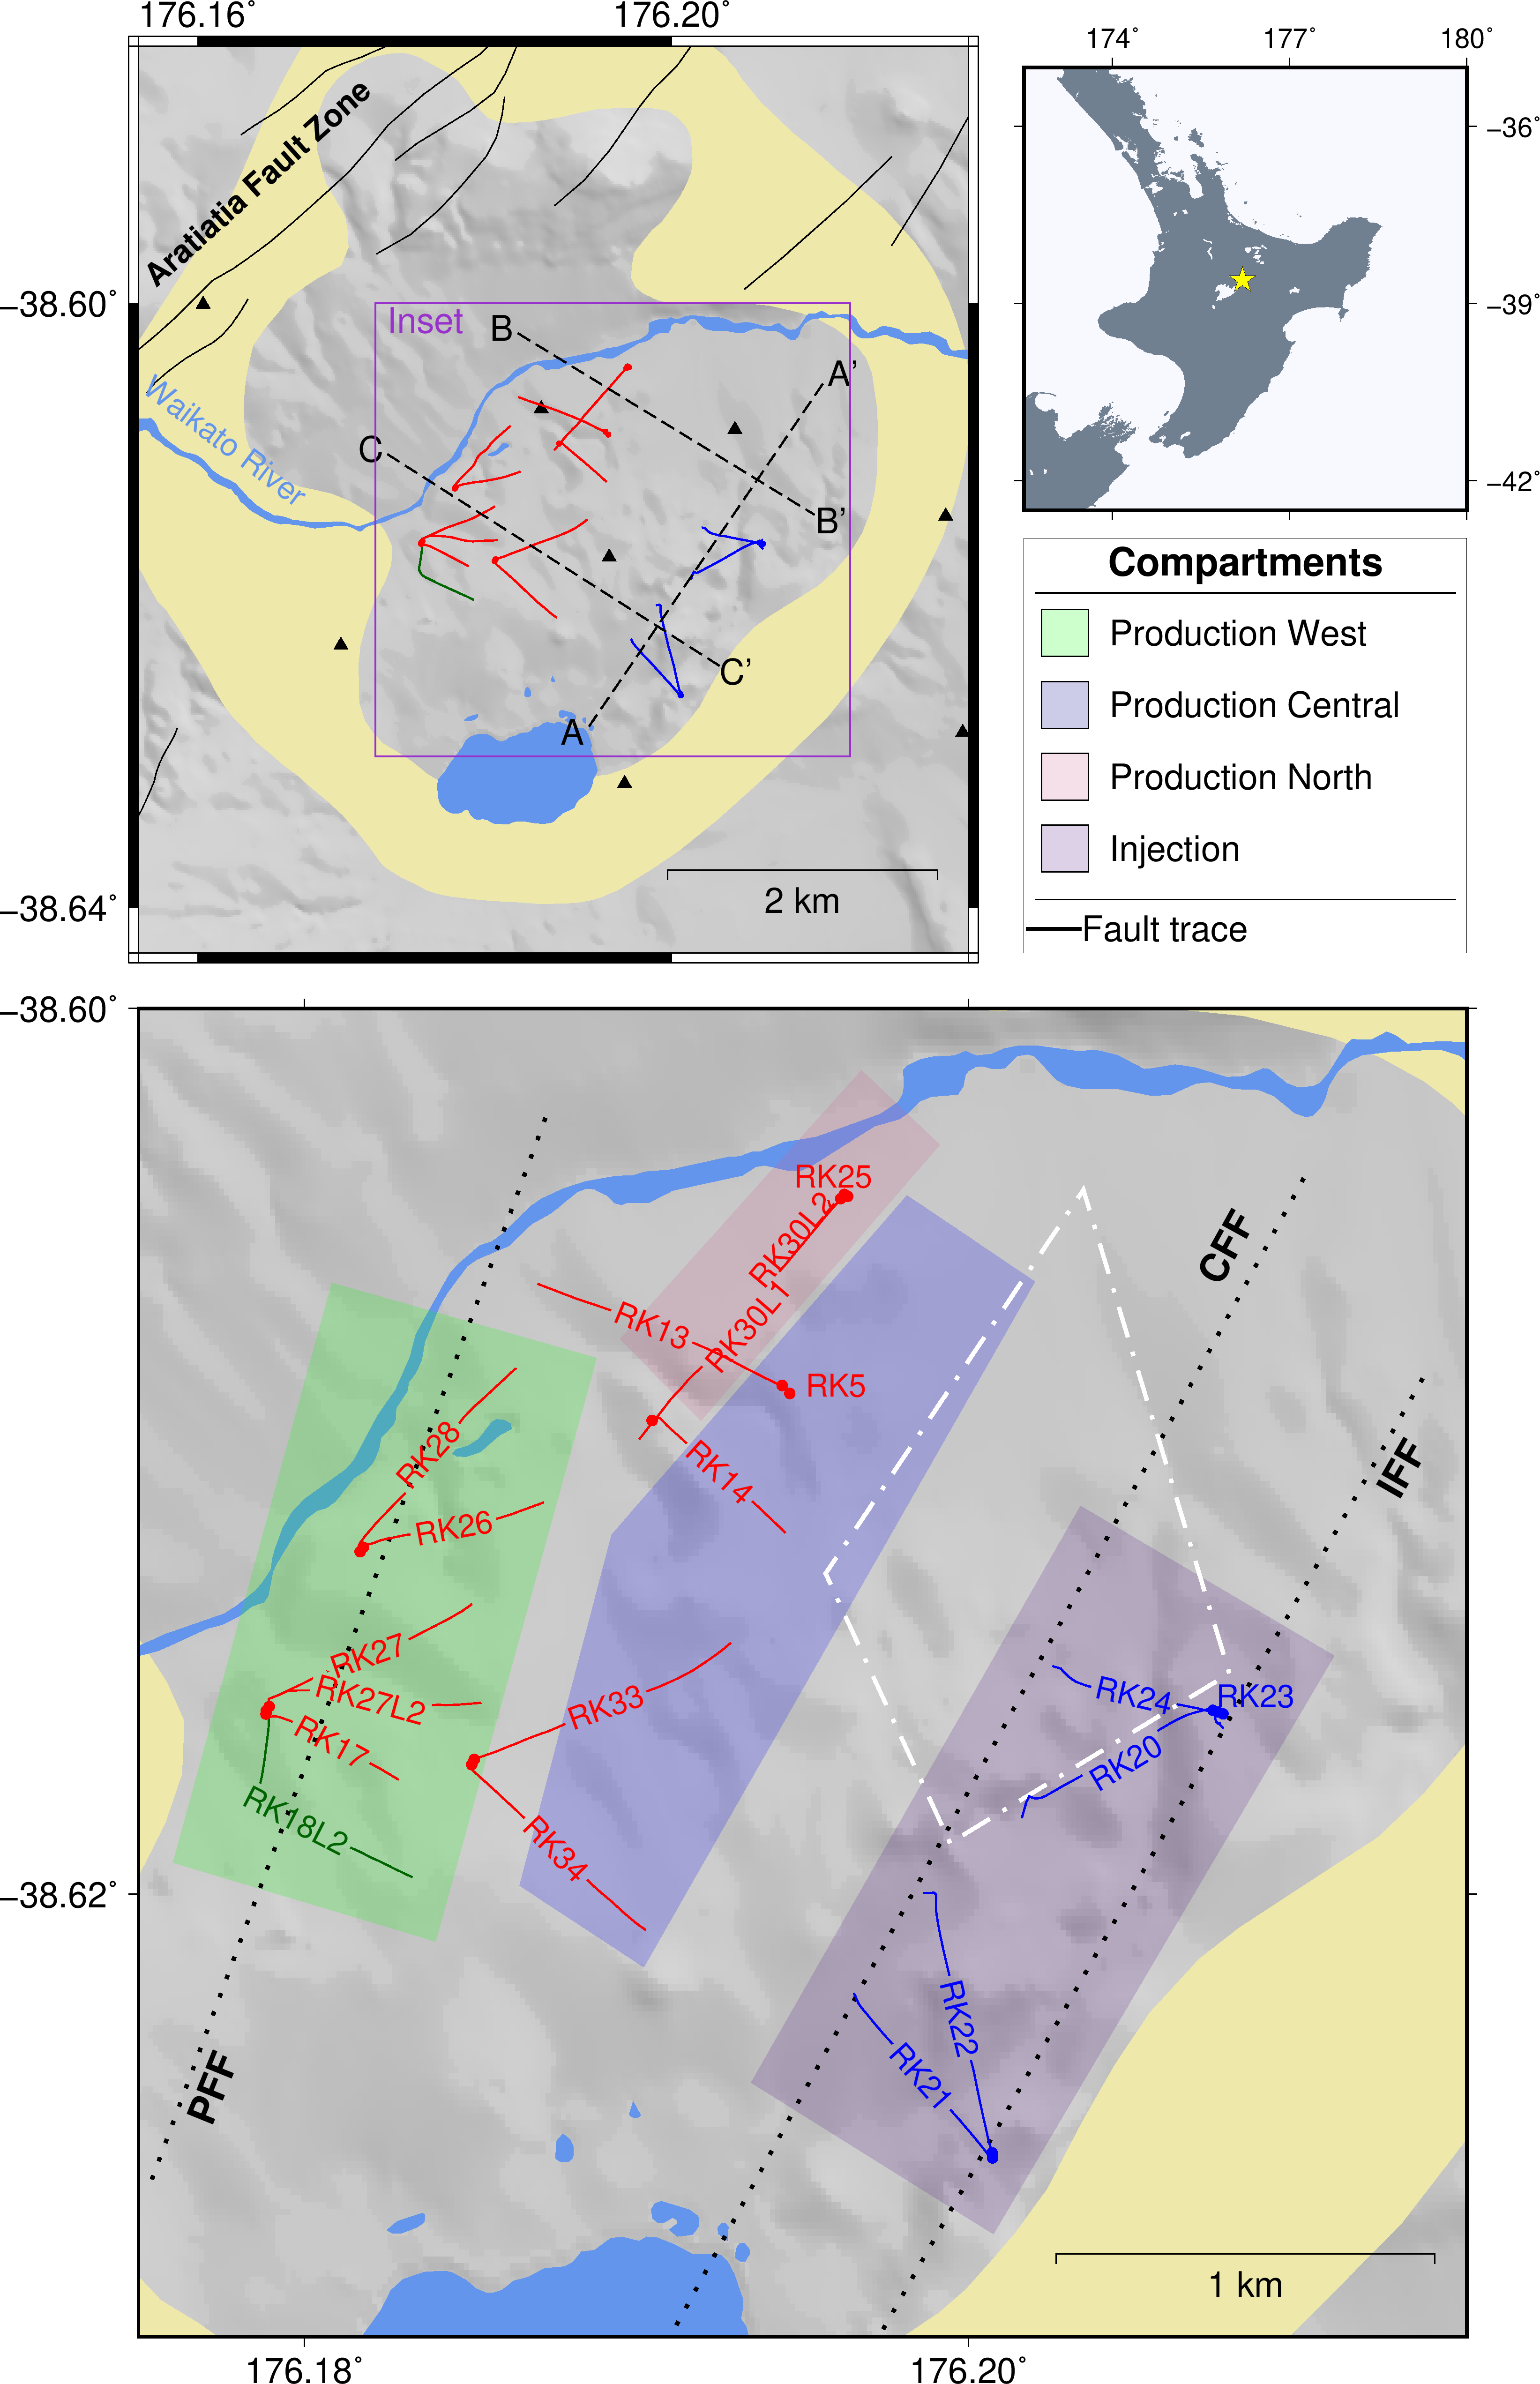
\includegraphics[width=0.73\columnwidth,height=\textheight,keepaspectratio]{Chapter_1_Intro/figures/merc_Rot_overview/merc_Rot_overview_struct_inset_NI_compartments}
\caption[Overview of the Rotokawa geothermal field]{{
Overview of the Rotokawa geothermal field. The top right panel shows the
location of the field on the North Island of New Zealand (yellow star).
The top left panel shows the resistivity boundary of the field in yellow
and injection, production and monitoring wells in blue, red and green, respectively. Solid
black lines are active faults. Dotted lines correspond to cross-sections A-A', B-B' and C-C' in Figures \ref{599670} and \ref{673646}. The lower panel shows a closeup of the
field, with the well names labeled and the three known faults (\acrshort{PFF}, \acrshort{CFF},
\acrshort{IFF}) shown as black dotted lines. The white dot-dashed line shows the
extent of significant seismicity from 2008-2012, as reported
by~\protect\citet{Sherburn_2015}. There are four known compartments in the Rotokawa
reservoir shown as colored polygons. Each is semi-isolated from the
others by either a \gls{permeability} contrast or impermeable barrier (i.e. a
fault). The production field comprises three compartments, the west,
central and north (green, blue and red, respectively). The injection
field is shaded in purple and is a separate compartment.
{\label{838185}}%
}}
\end{center}
\end{figure}\selectlanguage{english}

\begin{sidewaysfigure}[p]
\begin{center}
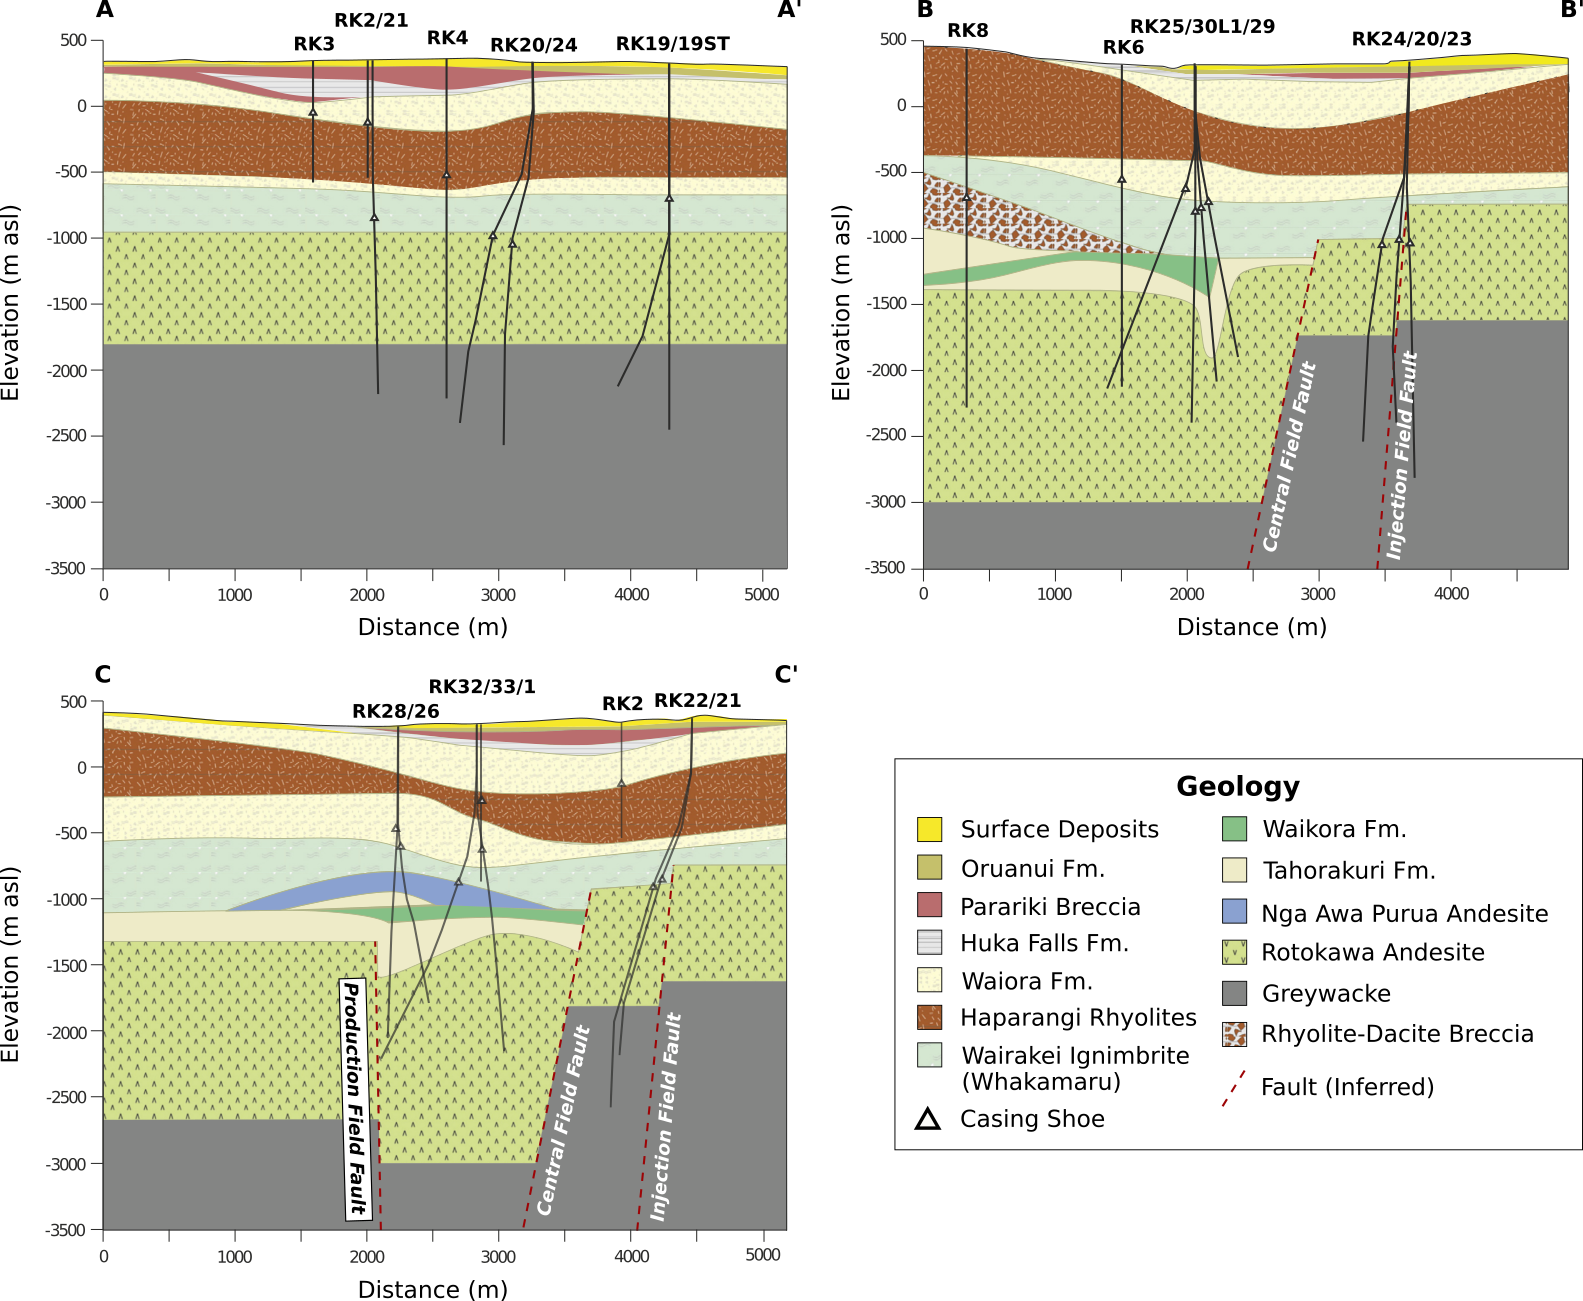
\includegraphics[width=0.66\textwidth,height=\textheight,keepaspectratio]{Chapter_1_Intro/figures/Rotokawa_geology_11-20/Rotokawa_geology_3-20}
\caption[Selected cross-sections of Rotokawa geology]{{
Three selected cross-sections showing the geology of the Rotokawa
geothermal field (modified from~\protect\citet{Sewell_2015} to correspond to
Figure {\ref{673646}})
{\label{599670}}%
}}
\end{center}
\end{sidewaysfigure}

\subsubsection{Development}
As at Ngatamariki, resource characterization at Rotokawa began with exploratory drilling by the New Zealand government, which confirmed the existence of the \textgreater300\textdegree C resource \citep{Sewell_2015,McNamara_2016}. The \acrfull{RGEN} was installed in 1997 with a capacity of 24 \acrshort{MWe}. During this phase of development, production and injection both occurred within the modern production field, with injection taking place between 500 and 1000 m depth \citep{Sewell_2015}. In 2000, production was increased to 34 \acrshort{MWe} and the shallow injection was moved to deeper wells on the southwest periphery of the production field (e.g. RK18) (Figure \ref{838185}). In 2007, the Rotokawa Joint Venture (Tauhara No. 2 Trust and Mercury) were granted consents to increase development at Rotokawa with the addition of the 138 \acrshort{MWe} \acrfull{NAP} triple-flash plant, which was commissioned in 2010 \citep{Sewell_2015}. With the drilling of wells RK19-RK30, the management strategy was shifted so that deep injection occurred to the southeast at wells RK20-RK24 and production came from the wells in the already-developed portions of the field (Figure \ref{838185}) \citep{Sewell_2015,McNamara_2016}. Requirements for further production prompted the drilling of wells RK32-RK34 following the startup of \acrshort{NAP} (Figure \ref{838185}).

During our study period (2012--2015), there were four main periods of interest identified by Mercury from a reservoir management perspective:
\begin{itemize}
  \item{\textbf{RK24 \Gls{injectivity} Decline}}
  
  Following \acrshort{NAP} startup, it was determined from radioactive tracer returns that the southern injection wells, specifically RK21, were producing rapid returns at the southern production wells \citep{addison2015rotokawa}. Injection was moved to northern injection well RK24 but within six months \acrshort{II} had begun to decline in the well (Figure \ref{701773}). Mercury have identified this as a time period of interest where patterns of seismicity may be able to inform the reason for this \gls{injectivity} decline.
  \item{\textbf{Switch of Injection: RK24-RK23}}
  
  Given the \acrshort{II} decline noted above, Mercury decided to shift some injection away from RK24 and into RK23 (June 2014). It is possible that this produced an accompanying change in seismicity (Figure \ref{701773}).
  \item{\textbf{RK34 Drilling Losses}}
  
  As with NM10 at Ngatamariki, total losses were incurred during the drilling of make-up production well RK34 (September to November 2014). As RK34 was drilled in the seismically-quiet production field, any accompanying seismicity may be more easily identified than in the injection zone.
  \item{\textbf{Plant Shutdowns and Startups}}
  
  For prior periods (i.e. before 2013), swarms of seismicity may have occurred in response to plant shutdowns and startups (typically for maintenance). These swarms have been attributed to transient pressure changes in the reservoir \citep{Sherburn_2015}, and Mercury have identified future plant shutdowns as periods of seismic interest.
\end{itemize}\selectlanguage{english}

\begin{figure}[p]
\begin{center}
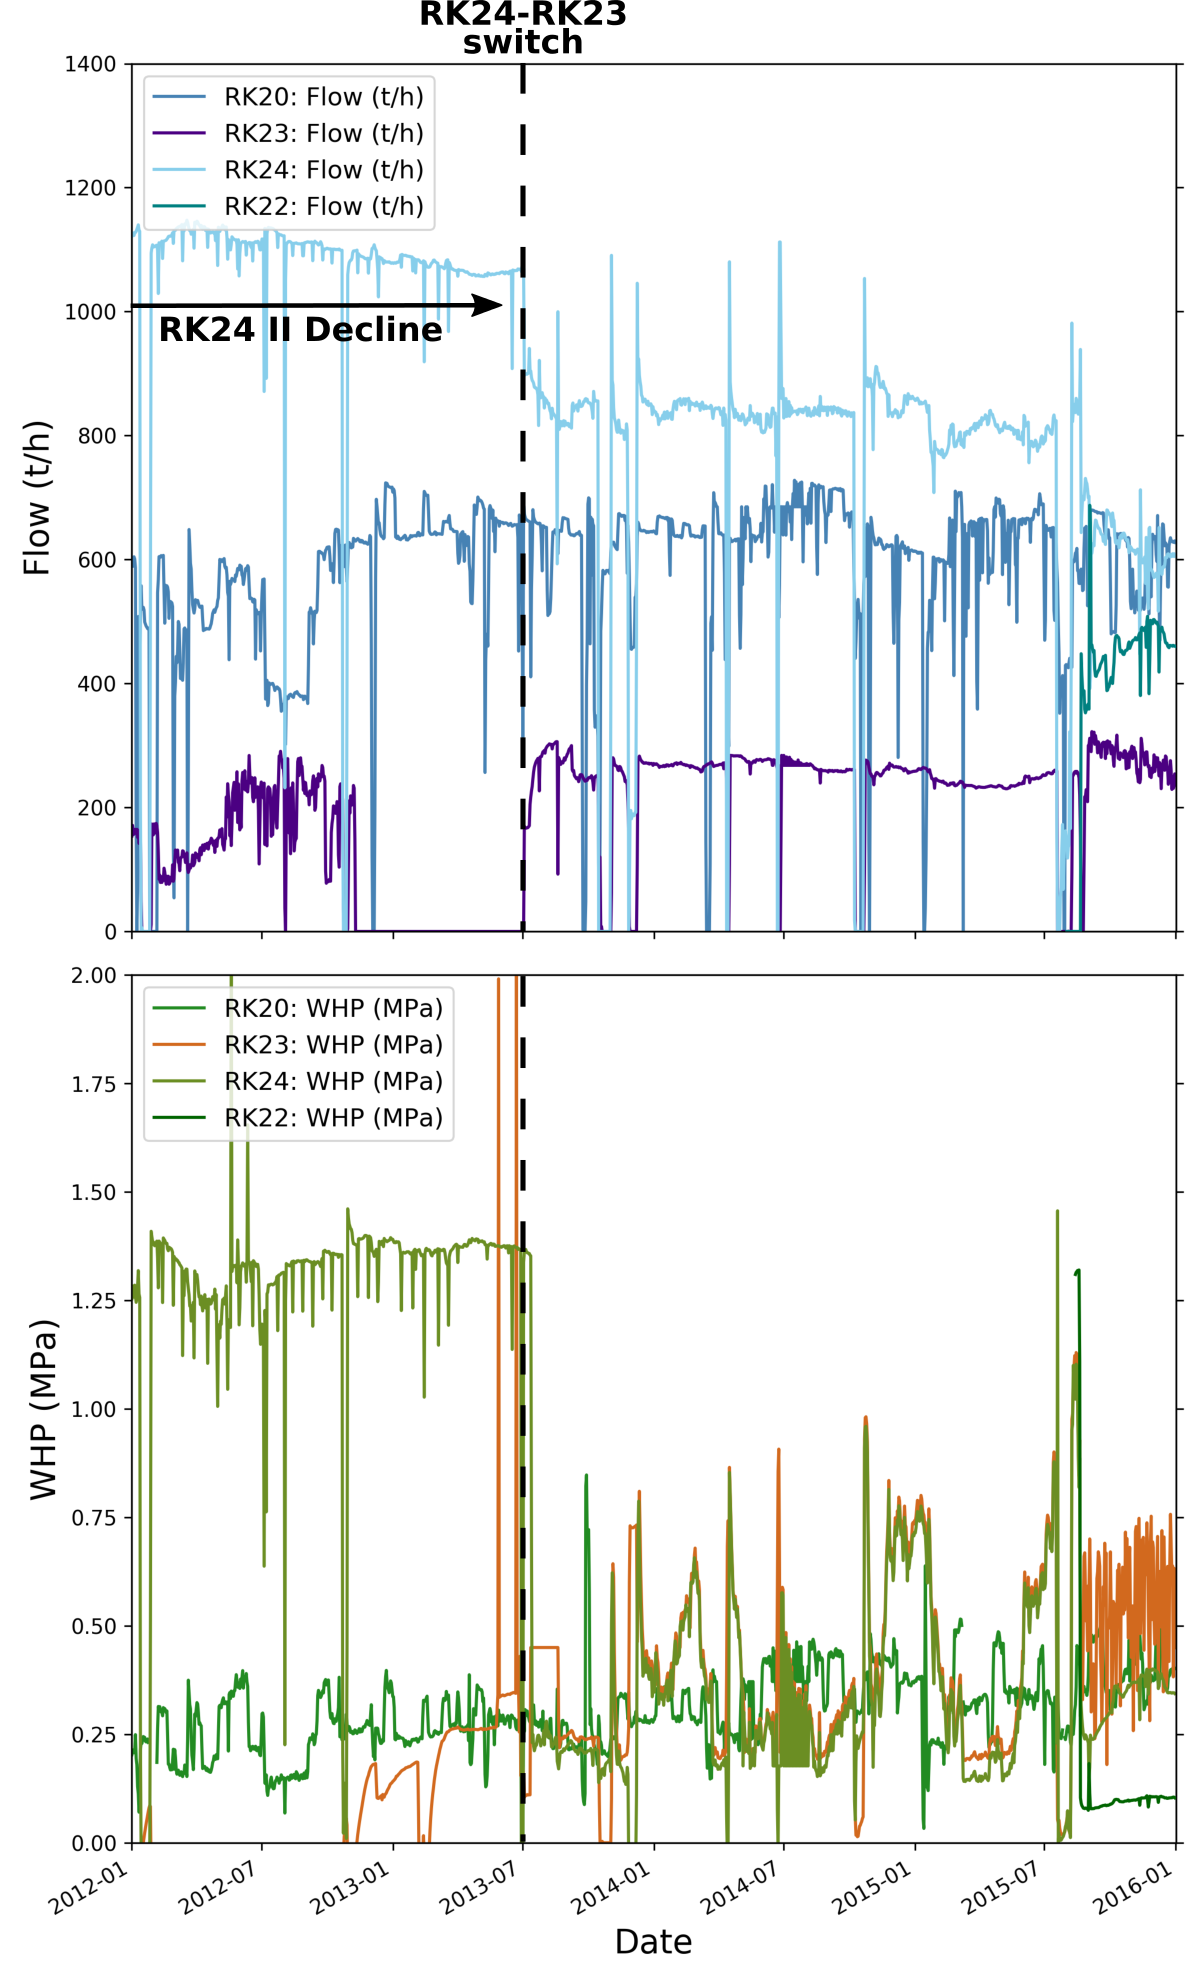
\includegraphics[width=0.82\columnwidth]{Chapter_1_Intro/figures/Rotokawa_overview_Intro/Rotokawa_overview_Intro_3-20}
\caption[Rotokawa flow rates and wellhead pressures: 2012--2015]{{
Overview of \glspl{flow_rate} (top panel) and \glspl{WHP_g} (bottom panel)
from 2012 through 2015 for deep injection wells at Rotokawa. Selected
periods of interest as identified by Mercury are annotated on the flow
rate panel. RK34 was drilled from September to November 2014, but is not noted here due to a lack of \gls{flow_rate} data.
{\label{701773}}%
}}
\end{center}
\end{figure}\selectlanguage{english}

\begin{sidewaysfigure}[p]
\begin{center}
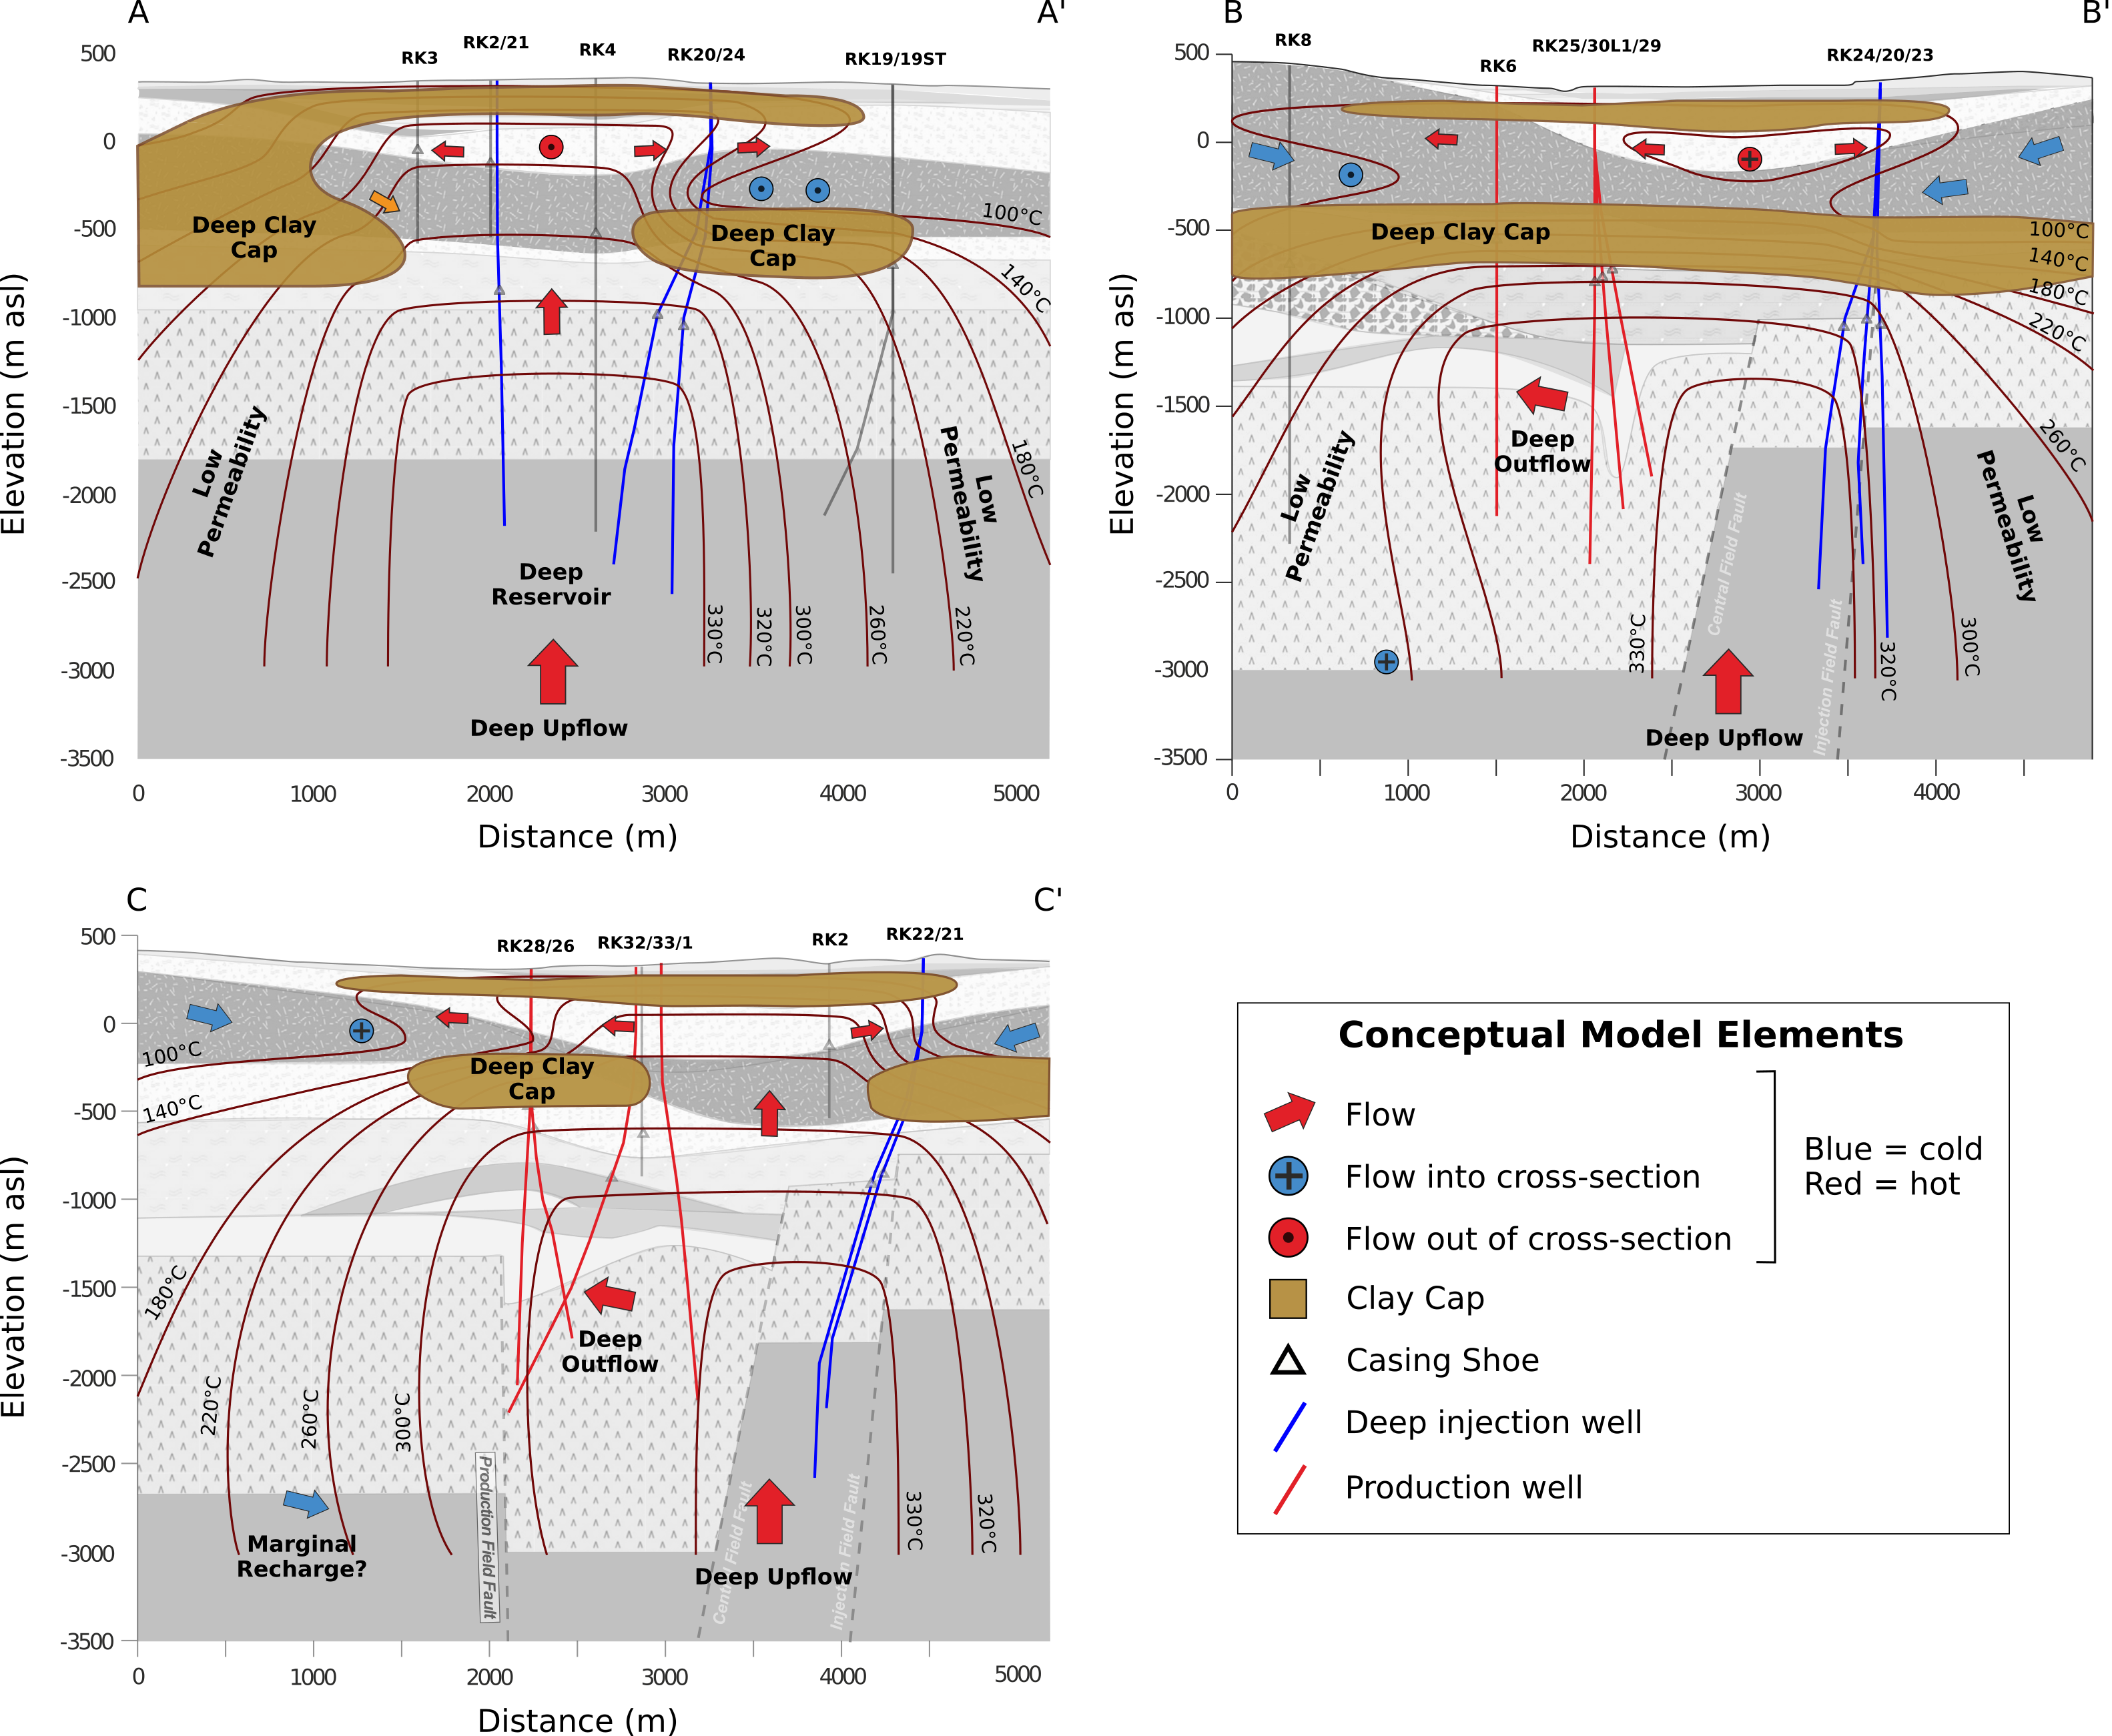
\includegraphics[width=0.63\textwidth,height=\textheight,keepaspectratio]{Chapter_1_Intro/figures/Rotokawa_conceptual_11-22/Rotokawa_conceptual_2-20}
\caption[Selected cross-sections of the Rotokawa conceptual model]{{
Elements of the current Rotokawa conceptual model
from~\protect\citet{Sewell_2015} overlain on the geologic cross sections shown in
Figure~{\ref{599670}}. Maroon lines are isotherms
modeled from well temperature profiles. Arrows show the direction and
temperature of flow in the current reservoir conceptual model
(blue=cold, red=hot).
{\label{889233}}%
}}
\end{center}
\end{sidewaysfigure}

\subsubsection{Conceptual Model}
The understanding of the Rotokawa reservoir has benefited from over 20 years of detailed study and characterization spanning two phases of development. As a result, the understanding of the reservoir and the nature of fluid flow is well developed \citep{Sewell_2015,Addison_2017stanford,wallis2013}. The hottest temperatures in the field are found in the southern injection zone, with a maximum temperature of 338\textdegree C measured in well RK22 (Figure \ref{838185}), but there are strong lateral gradients in the natural-state temperatures to the northeast and northwest \citep{Sewell_2015,wallis2013} (Figure \ref{889233}). The main upflow of \textgreater330\textdegree C fluid is located near wells RK21\slash{RK22}, although the southwest extent of the reservoir and upflow has not been verified by drilling \citep{Sewell_2015,winick2011natural}. Similar to Ngatamariki, Rotokawa is overlain by intermediate and shallow aquifers. However, the hydraulic connection between the deep reservoir and intermediate aquifer at Rotokawa is more pronounced than the `leak' at Ngatamariki \citep{winick2011natural} (Figure \ref{889233}).

At Ngatamariki, fluid flowing from injection to production travels N-S, oblique to the regional NE-SW structure. At Rotokawa, the injection-production flow path is oriented NW-SE, perpendicular to the structural trend. This geometry has implications for fluid flow through the reservoir as faults (in this case) act as along-strike flow pathways and cross-strike flow barriers \citep{Addison_2017stanford,McNamara_2015,Sewell_2015}. The effects of these structural barriers can be seen across the field. The \acrfull{CFF} effectively isolates the injection and production zones, allowing only $\sim$12\% of the tracer injected in the injection wells to return to the production field within 60 days \citep{Sewell_2015,addison2015rotokawa}. Similar \glspl{tracer_test} have shown the \acrfull{PFF} to be a conduit for rapid along-strike flow within the production field, resulting in the extraction of cool fluid and the shift of deep injection from the southwest production field to the current injection zone \citep{Sewell_2015,Addison_2017stanford}. The \acrfull{CFF} is also inferred to be the structure that controls the connection between the deep and intermediate aquifers, and its surface trace appears to control the locations of a number of features (i.e. hot springs and geysers) at the field \citep{winick2011natural}.

Patterns in pressure drawdown in the production field are elongate along-strike, also suggesting that fluid flow is restricted across the structural grain \citep{hernandez2015rotokawa,Sewell_2015,Quinao_2013stanford}. The magnitude of these pressure differentials suggests a high degree of compartmentalization in the reservoir (Figure \ref{838185}). For instance, the pressure drawdown at RK29 since commissioning of \acrshort{NAP} was $\sim$0.4 \acrshort{MPa} as of 2015. However, at RK25\slash{RK30}, which are only $\sim$200 m from RK29, the pressure drawdown is roughly an order of magnitude greater, despite the fact that RK29 extracts more fluid than any other well in the field \citep{Sewell_2015}. Similar NW-SE pressure differentials exist in the southwestern production field and the variations in pressure responses across the entire production field suggest at least three separate compartments \citep{hernandez2015rotokawa}. The currently accepted boundaries of the three production field compartments, as well as the injection field, which comprises a separate compartment, are shown in Figure \ref{838185}.

\subsubsection{Seismicity}
Workers at GNS Science and Mercury (Mighty River Power) examine the seismicity at Rotokawa on a yearly basis in an effort to monitor changes in the reservoir. However, the last detailed characterization was only conducted through 2012 \citep{Sewell_2015WGC,Sherburn_2015}. As expected, seismicity migrated in conjunction with evolving injection strategy. At the end of 2012, with injection occurring predominantly into the southeastern compartment of the reservoir, \citet{Sewell_2015WGC} and \citet{Sherburn_2015} observed that seismicity occurred inside the white dotted diamond shown in Figure \ref{838185}, migrating from the southern half of the diamond in 2008 to the northern half by 2012. The location of the northwest segment of this diamond has also been used to infer the location of the \acrshort{CFF}. In addition, \citet{Sewell_2015WGC} and \citet{Sherburn_2015} concluded that seismicity at Rotokawa was induced mostly by stress changes associated with reservoir cooling and contraction, instead of by pore-pressure increase, due to the relatively small pressure buildup measured at the wells (no greater than 1.5 \acrshort{MPa}). In the analysis that follows, specifically in Chapters 4 and 5, we look to update this understanding of Rotokawa seismicity.

\section{Induced Seismicity}\label{IS}
Human-induced seismicity was first recognized decades ago, but has received a large amount of attention recently due to a remarkable increase in the number of events in the central US and elsewhere \citep{Ellsworth_2013,Kim_2013,Keranen_2013,Kim_2013,Keranen_2013,Zoback_2012co2,Baisch_2006,Evans_2004,Deichmann_2009}. Human-triggered seismicity has in fact been observed for nearly a century in relation to the impoundment of large water reservoirs \citep[e.g.][]{carder1945seismic,Gupta_2018} and early oil and gas operations \citep{Hough_2016}. Following a high-profile case of IS at the Rocky Mountain Arsenal near Denver, CO in 1962 \citep{Healy_1968}, a controlled experiment at the Rangely oil field in Colorado demonstrated a convincing connection between fluid injection and seismicity \citep{Raleigh_1976}. Also, starting in the 1960's, new hydraulic fracturing (i.e. `fracking') techniques were being used to rehabilitate old oil and gas reservoirs, but these operations garnered little attention as the volumes injected were relatively small and the targeted formations were relatively permeable, leading to little notable seismicity. In the 1990's, however, the combination of massive hydraulic fracturing and advances in horizontal drilling made possible fracking in tight, shale reservoirs and opened large parts of the aseismic interior US to large-volume fluid injection. The rapid deployment of these techniques in places such as Oklahoma, Ohio and Texas brought about noticeable increases in felt seismic events in these areas \citep{Ellsworth_2013} that have since been attributed to the injection of fracking wastewater and to fracking itself \citep[e.g.][]{Kim_2013,Keranen_2013,Kim_2013,Keranen_2013}.  These events heightened international attention for the topic of IS and spurred a continuing effort to understand what factors determine where and when injection operations will induce seismicity \citep[e.g.][]{Goebel_2018}.

\subsection{Settings of Injection IS}
Human-induced seismicity is related to a number of processes including mining or gas-related mass extraction and weapons testing \citep[e.g.][]{Chambers_2015,Kim_2007}. Here, however, we focus on IS related to the injection of fluids into the subsurface, which generally occurs in three settings:
\begin{itemize}
  \item{\textbf{Oil and Gas Extraction}}
  
  As mentioned above, the bulk of the attention devoted to IS internationally is related to enhanced oil and gas recovery through massive hydraulic fracturing. Certain cases have been directly attributed to the hydraulic fracturing treatments themselves \citep[e.g.][in Canada]{Atkinson_2016,Skoumal_2015}. However, the vast majority of cases are induced by the deep disposal of fracking-related wastewater at or below the depths of the fracking wells \citep[e.g.][]{Kim_2013,Keranen_2013,Yeck_2017,McGarr_2017}. Many of these events are located at depths below that of the injection and occur on preexisting basement faults up to tens of km away from the injection well. The factors that determine whether seismicity will occur for a given scenario, and what the frequency and magnitude might be, are still a topic of active research.

  \item{\textbf{CO$_{2}$ Sequestration}}
  
  Over the past decade, the possibility of capturing CO$_2$ produced by industrial activities and reinjecting it into the subsurface has been raised as a potential strategy for mitigating human-induced climate change. As a result, a number of pilot projects exploring the efficacy of carbon capture and storage have been undertaken in various locations worldwide \citep{Evans_2012,Zoback_2012co2}. This process involves the injection of liquid (supercritical) CO$_2$ into the subsurface, and therefore may generate seismicity via the same processes involved with fracking and wastewater disposal \citep{2013}. Currently, the future risk of induced seismicity associated with these projects is difficult to determine. If this technology is to be adopted as a viable climate-change mitigation strategy, it will involve injected volumes many orders of magnitude larger than those related to the current pilot projects \citep{Zoback_2012co2}. However, even at these relatively small volumes, significant seismicity has been recorded in some locations \citep[e.g.][]{Goertz_Allmann_2017}.
  
  \item{\textbf{Geothermal Power Production}}
  
  As described above, power can be produced by `mining' heat from deep reservoirs in the earth's crust. These reservoirs can be divided into enhanced geothermal systems (EGS) and conventional reservoirs. In this thesis, we will deal with conventional reservoirs. However, the seismicity induced at EGS reservoirs is still relevant to the discussion of injection-induced seismicity, especially in medium to high-temperature reservoirs.
  
  The aim of EGS is to mine heat from hot, yet relatively impermeable, rock at drilling-accessible depths. Usually, this is accomplished through injection of fluids at pressures sufficient to fracture rock (similar to oil and gas fracking) and/or shear preexisting faults and fractures in the reservoir (sometimes called `hydroshearing`), thereby creating a permeable reservoir between an injection and production well (or wells). Enhanced geothermal systems came about as part of the Hot Dry Rock experiment in the 1970's by the Los Alamos National Laboratory \citep{2013} in New Mexico. Subsequent projects were undertaken in England, France, Germany and Japan, with varying degrees of success and in the last 15 years other projects have been undertaken in Australia, Sewden and Switzerland. In each of these cases, some amount of seismicity was induced \citep{2013,Baria_1989,Baisch_2006,Evans_2004,Deichmann_2009}.
  
  Conventional geothermal reservoirs are those which already have sufficient heat and \gls{permeability} for a convective hydrothermal system to have developed \citep{Grant_2011}. In these cases, extraction of fluid for power production is relatively easy, as no \gls{permeability} need be created. However, extraction of fluid can also deplete the resource, causing surface subsidence and pressure drawdown \citep{Grant_2011}. Fluid is therefore reinjected into the reservoir as a means of pressure support and as a mitigation strategy against resource depletion. Conventional reservoirs are mostly located in areas of active tectonics such as New Zealand, Iceland, Italy, the Phillipenes, Indonesia, California and Central America and have been associated with seismicity for decades \citep[e.g.][]{Batini_1985,Allis_1982}. Rotokawa and Ngatamariki are both high-temperature, fluid-dominated versions of the conventional geothermal reservoir and so are most directly comparable to these types of fields elsewhere.
\end{itemize}

\subsection{Mechanisms of IS}\label{mechanisms}
Slip occurs on a fracture or fault when the shear force acting upon it exceeds its frictional strength \citep{stein_2000}. This condition can be met through an increase in the shear stress or a decrease in the frictional strength. The conventionally-accepted mechanism by which seismic slip is induced during fluid injection operations is the increase in pore fluid pressure (Figure \ref{469299}), which decreases the normal stress on the fracture, thereby reducing its frictional strength and allowing a rupture to nucleate \cite[e.g.][]{Majer_2007}. However, as has become more clear with the growing number of case studies, there are other process that play important roles in IS and interact in ways that are complex and poorly understood. The key mechanisms that induce seismicity during fluid injection include:
\begin{itemize}
  \item{\textbf{Pore-fluid Pressure Perturbation}}
  
  The simplest explanation for the occurrence of IS is pore-fluid pressure increase within a fracture network that is hydraulically connected to the injection well. In such a scenario, any pressure perturbation at the well diffuses through the fracture network at a rate that depends on hydraulic properties of the reservoir, specifically hydraulic \gls{diffusivity}, $D$ (Section \ref{terms}). \citet{Shapiro_2002} developed a technique called seismicity-based reservoir characterization (SBRC) by which the hypocentral locations of induced events could be used to infer the hydraulic \gls{diffusivity} of a reservoir. This technique is based on the assumption that IS is induced purely as a result of the pore-fluid pressure increase, originating at an injection well and diffusing outwards. This is sometimes referred to as the slow `Biot wave' \citep{Biot_1956}. The outward diffusion of fluid molecules defines an envelope of $r = \sqrt{4\pi{D}t}$ for homogeneous, isotropic media, within which elevated pore pressure decreases the effective normal stress acting on a fracture network. As a result, the entire network is brought closer to failure and seismicity is most likely to occur, especially on structures that were already critically-stressed. This technique has been shown to be effective at describing the spatio-temporal occurrence of seismicity for numerous injections \citep[e.g.][]{Shapiro_1997,Shapiro_2009,Parotidis_2004,Jeanne_2014} (Figure \ref{182804}). However, it must be noted that this approach ignores the possibility of triggering by poroelastic stress transfer or thermal stress changes.
  
  Recently, however, \citet{cappa2019stabilization} have shown that elevated fluid pressures may actually encourage rate-strengthening behavior in a fault zone. If this is indeed the case, the zone affected by pore-fluid pressure increase does not correspond to the seismically-active zone at all, and seismic slip (requiring rate-weakening behavior) presumably occurs due to stable (aseismic) sliding transferring stress onto further portions of a fault. This finding may require rethinking SBRC, specifically, and pore-pressure as a triggering mechanism more generally.
\end{itemize}\selectlanguage{english}

\begin{figure}[h!]
\begin{center}
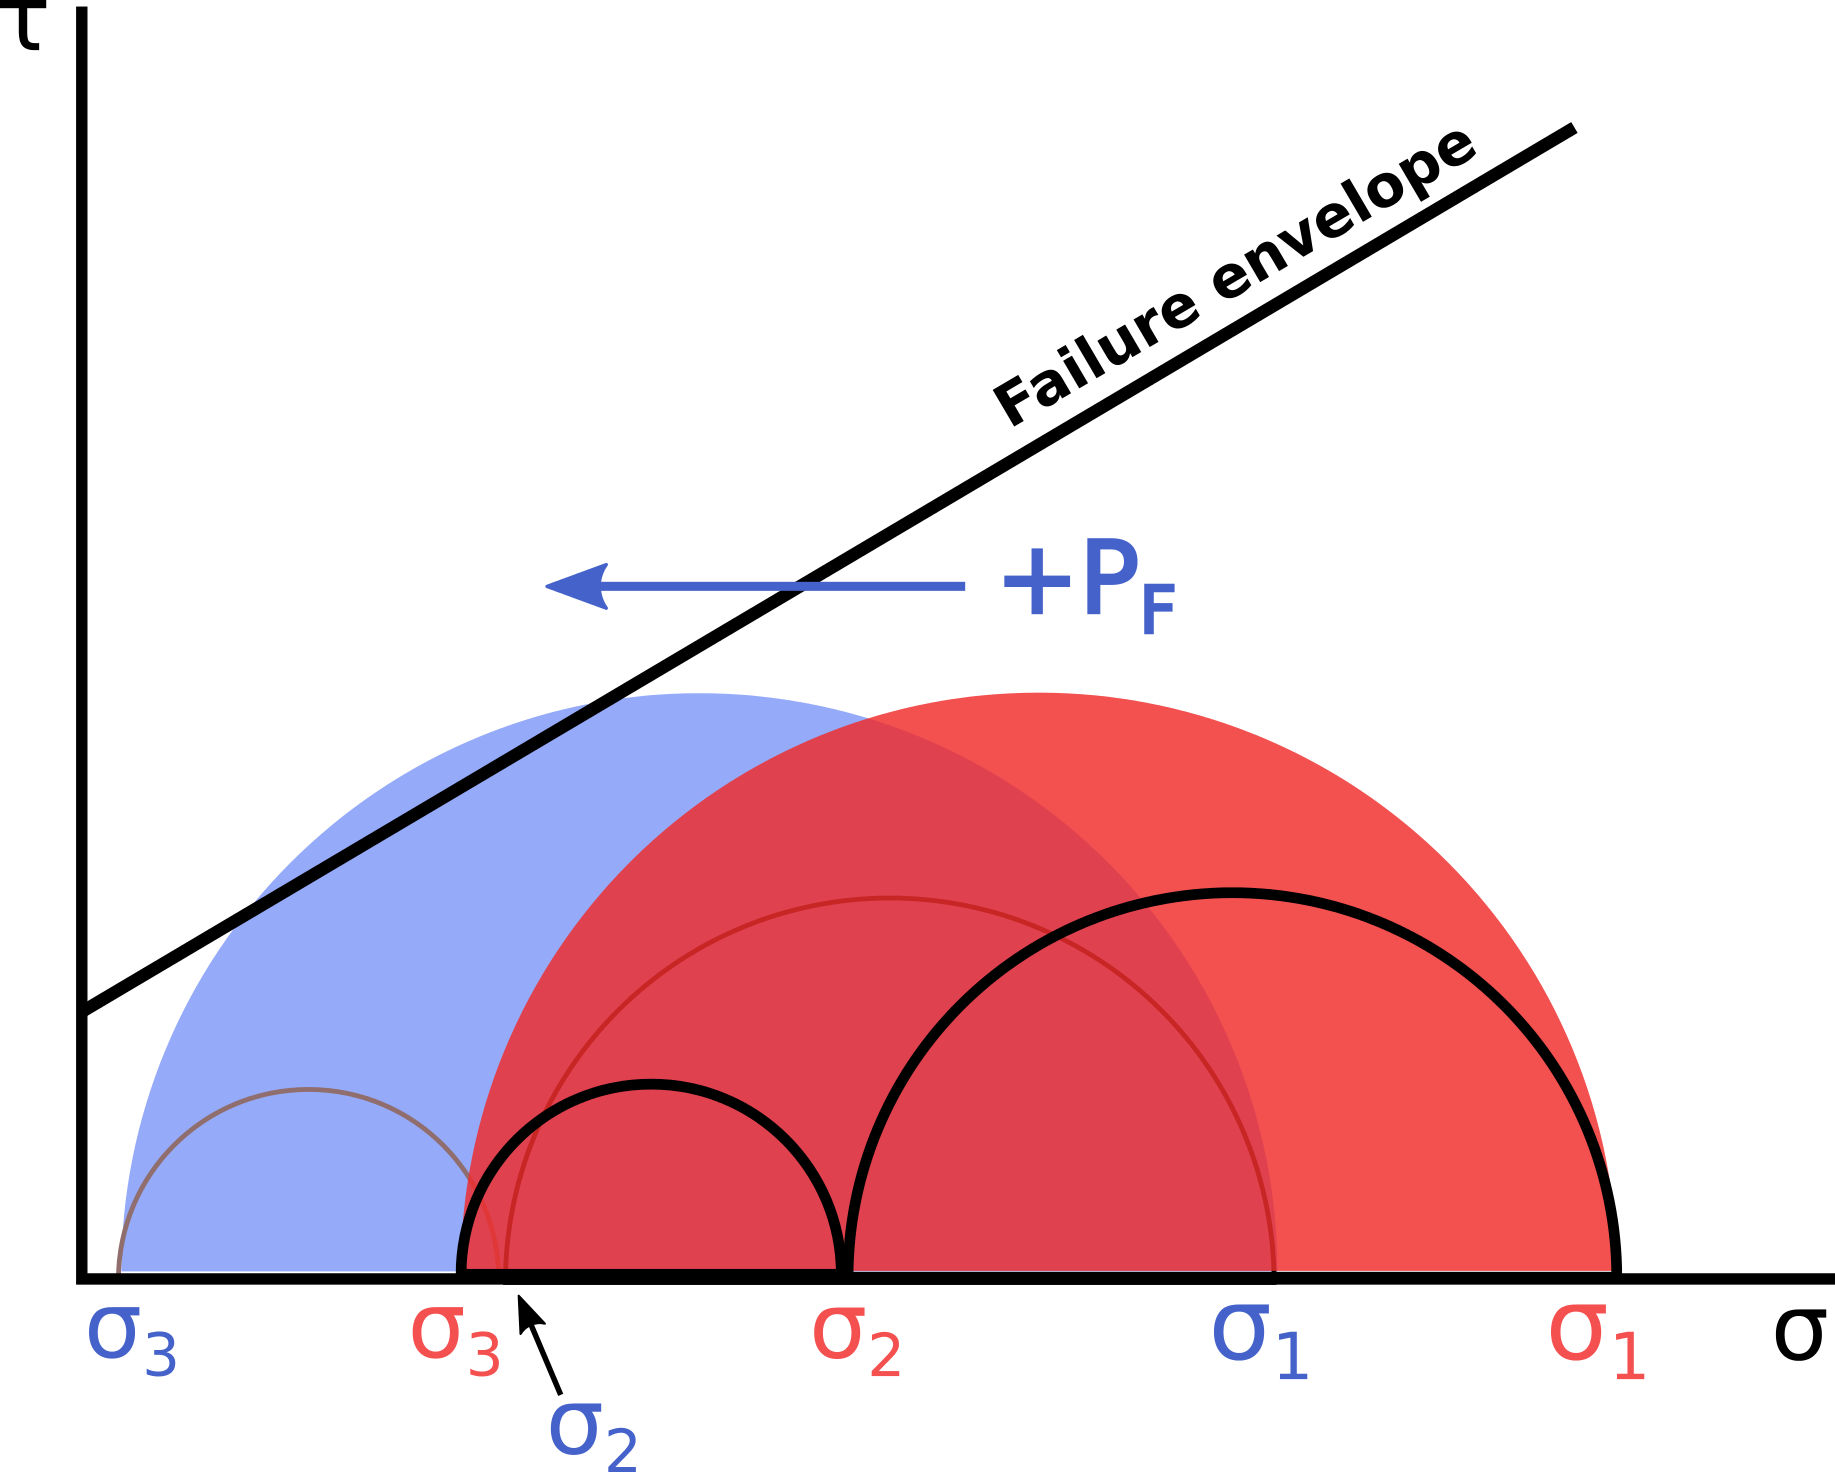
\includegraphics[width=0.7\columnwidth]{Chapter_1_Intro/figures/Pf_increase_mohr/Pf_increase_mohr}
\caption[Mohr circles showing the effect of pore-fluid pressure]{{
For a given stress tensor, the 3D Mohr's diagram comprises three circles, the largest of which has a diameter equal to $\sigma_{1} - \sigma_{3}$ (differential stress) and the two inner circles have diameter $\sigma_{1} - \sigma_{2}$ and $\sigma_{2} - \sigma_{3}$, from right to left. Any given plane can be plotted as a point above the smaller circles and below the largest according the normal ($\sigma$; x-axis) and shear ($\tau$; y-axis) tractions acting on it. When this point plots above the Mohr-Coulomb failure envelope, plotted as an arbitrarily-sloping black line, the plane is in disequilibrium and will fail. Here we show an unperturbed stress tensor in red, and the same tensor when a positive change in the pore-fluid pressure (P$_{f}$) is applied (blue). This has the effect of equally lowering the magnitudes of each principal stress, shifting the Mohr's circle to the left and, in this case, resulting in a population of planes above the failure envelope, which are suitable for failure (if they exist).
{\label{469299}}%
}}
\end{center}
\end{figure}\selectlanguage{english}


\begin{figure}[h!]
\begin{center}
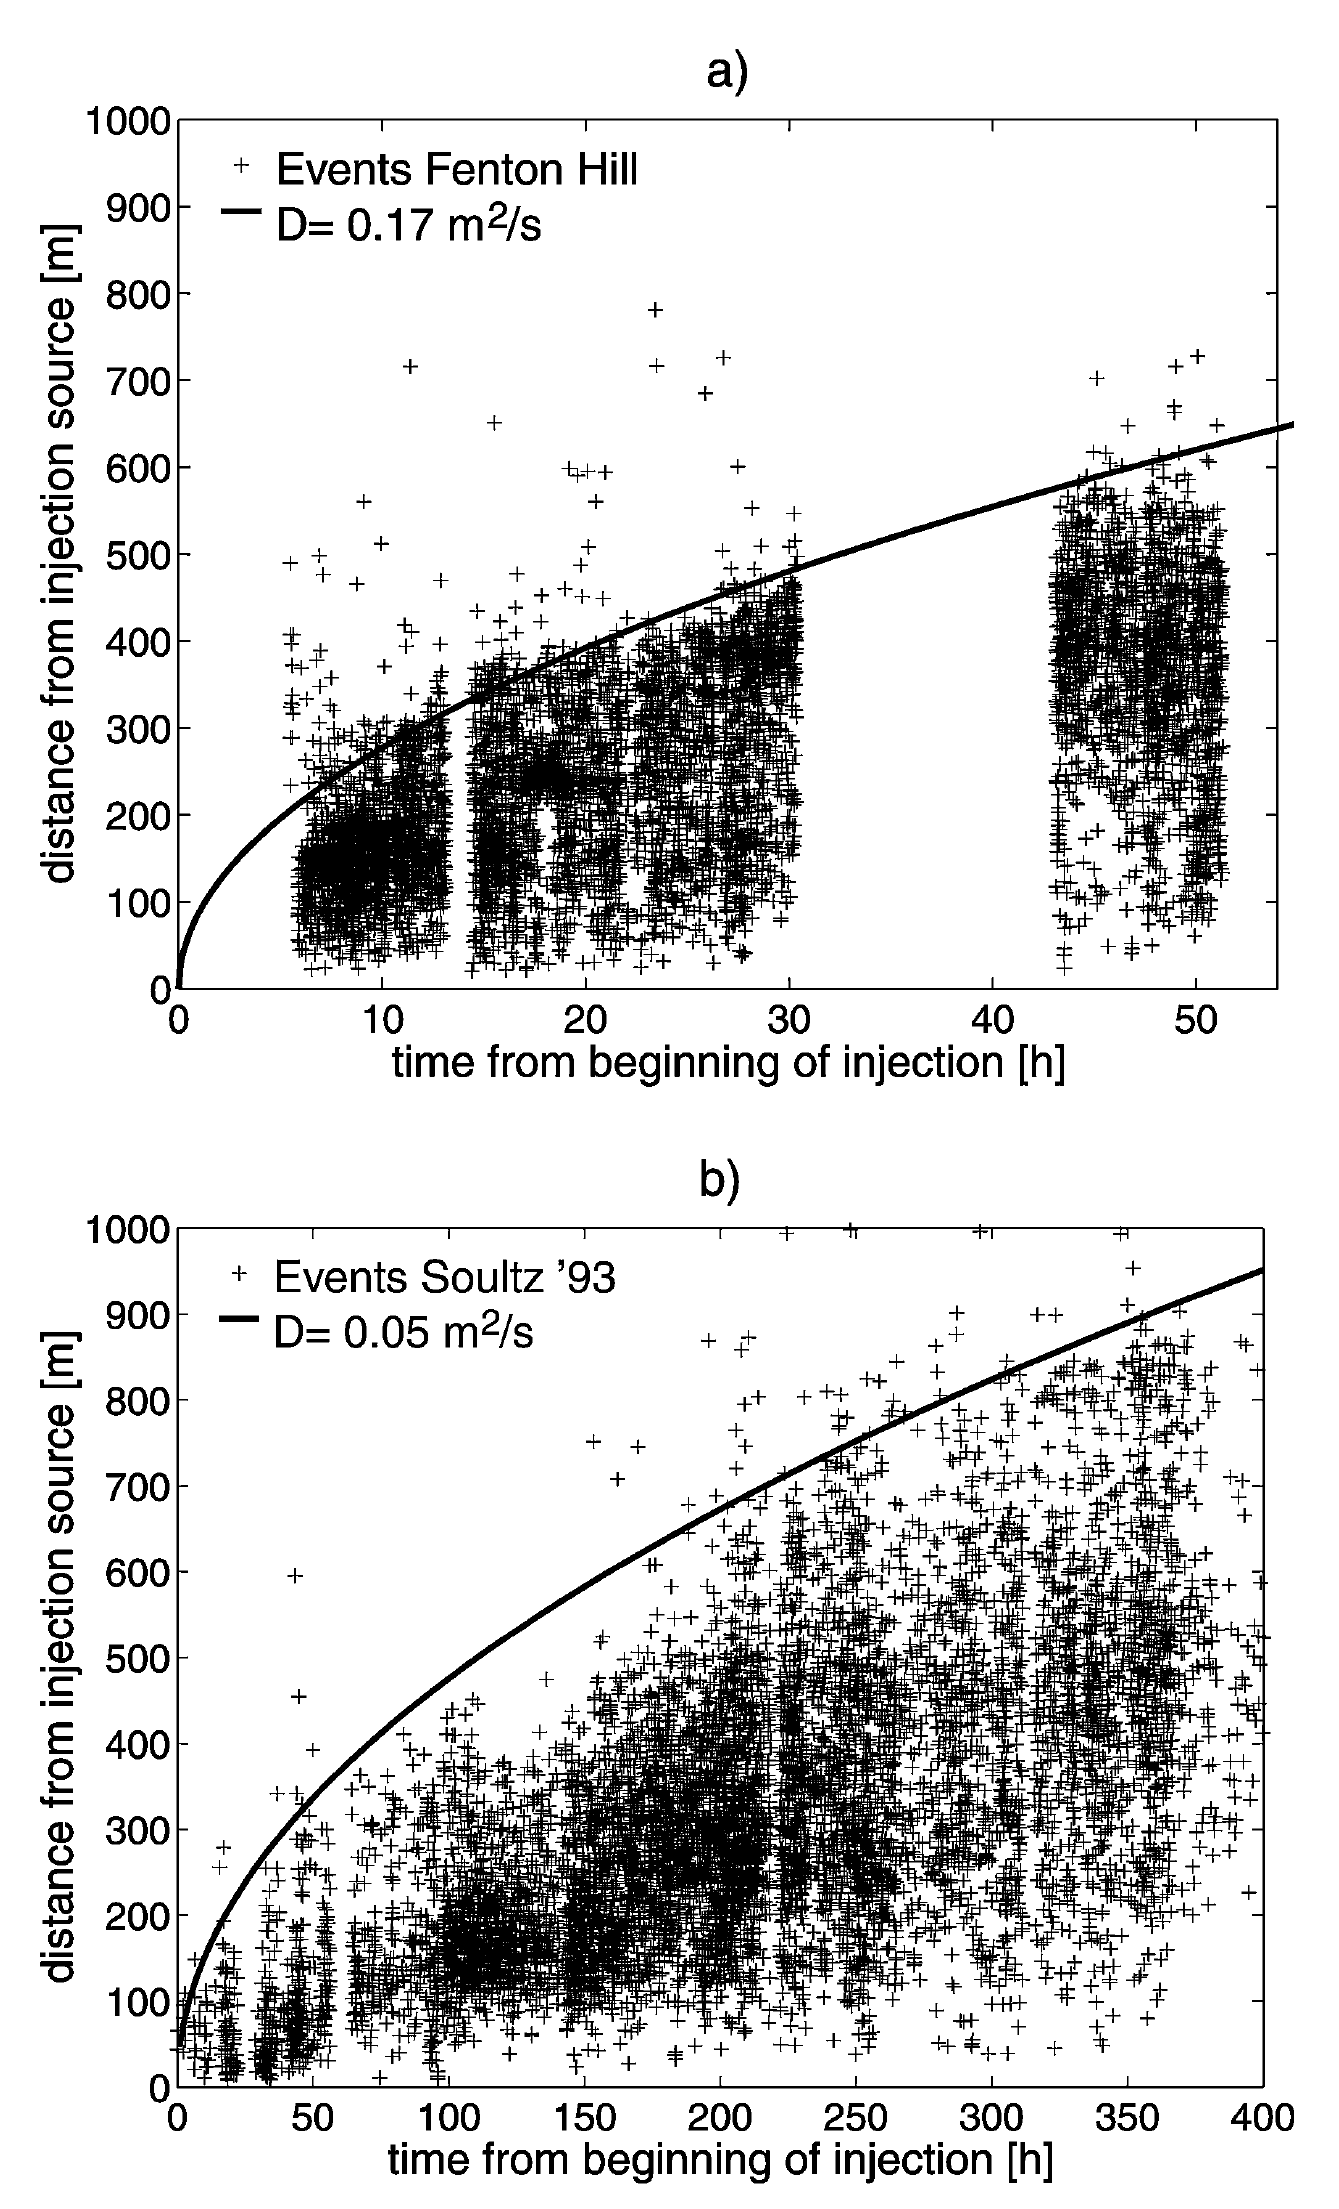
\includegraphics[width=0.70\columnwidth]{Chapter_1_Intro/figures/Shapiro_2002_SBRC_fig2/Shapiro_2002_SBRC_fig2}
\caption[Example `r-t' plot modified from \citet{Shapiro_2002}]{{
Typical `r-t' plots from~\protect\citet{Shapiro_2002} showing the triggering front
of seismicity as defined by SBRC for two injection operations: a) the
Fenton Hill, New Mexico Hot Dry Rock experiment and b) the Soultz EGS
project in France. Both sequences are well described by homogenous,
isotropic triggering fronts.
{\label{182804}}%
}}
\end{center}
\end{figure}

\begin{itemize}
  \item{\textbf{Poro-elastic Stress Transfer}}
  
  In addition to the perturbation of pore-fluid pressure, removal or injection of the large amounts of fluid from the subsurface induces related, and non-negligible, elastic stress changes due to the volume change of the reservoir \citep{2013}. In the case of depleted oil and gas reservoirs, or certain geothermal fields, this process can involve compaction of the reservoir and induce slip either within or outside the reservoir, depending on the prevailing tectonic regime \citep{Segall_1994,Segall_1998}. Where fluid is being injected into the reservoir, the corresponding increase in volume also induces a stress change. In the near-field (100s of m), the pore-fluid pressure increase experienced by fractures that are hydraulically connected to the injection well dominates the stress induced by volume change \citep{2013}. However, poroelastic stress transfer has been shown to dominate at greater distances and therefore, should not be ignored in assessing the effect of injection on IS \citep{Goebel_2017}. Recently, \citet{Goebel_2018} suggested that the degree to which either pore-pressure changes or poroelastic response dominate the seismic sequence is determined by the depth of injection with respect to basement. In their study, sub-basement injections were dominated by pore pressure increases and the associated seismicity terminated abruptly away from the well, whereas above basement injections were dominated by poro-elastic stress transfer and therefore had much wider spatial footprints and triggered larger magnitude events for a given injected volume \citep{Goebel_2018}. However, \citet{Hincks_2018} modeled the correlations between IS and a large number of operational and geological parameters for induced seismic sequences in Oklahoma and found a significant negative correlation between above-basement depths and seismic moment release. 
  
  An additional consideration for any seismic sequence, whether natural or induced, is the static (Coulomb) stress transfer associated with slip \citep{okada1992internal}. Coulomb stress change is known to explain the migration of aftershock sequences \citep[e.g.][]{Toda_2003}. It has also been shown to affect sequences of induced seismicity during EGS projects \citep{Catalli_2016,Schoenball_2012}. As mentioned above, modeling, lab and decameter-scale experiments recently reported by \citet{cappa2019stabilization} suggest that coulomb stress transfer may actually be the dominant mechanism responsible for induced seismic slip with elevated pore pressures instead inducing stable, aseismic sliding near the wellbore.

  \item{\textbf{Thermo-elastic Stress Transfer}}
  
  Finally, particularly when considering IS in geothermal reservoirs, thermoelastic effects are of paramount importance. A number of researchers, working at The Geysers geothermal field in northern California, have shown that injection-related cooling of the reservoir can induce large changes in the stress state that affect the style and location of induced faulting \citep{Mart_nez_Garz_n_2014,Mart_nez_Garz_n_2013,Mart_nez_Garz_n_2017,Jeanne_2014,Jeanne_2015tensor}. This effect is less pronounced, or negligible for injection scenarios where the temperature contrast between the reservoir and injected fluid is small, but in the case of high-temperature geothermal fields (including Rotokawa and Ngatamariki), the contrast can be 200--300\textdegree C \citep[e.g.][]{Mart_nez_Garz_n_2014,Jeanne_2015tensor}. Figure \ref{621452} illustrates the effect of thermoelastic stress reduction on the stress state in a reservoir from a Mohr-Coulomb perspective. The key point, as explained by \citet{Jeanne_2014,Jeanne_2015tensor}, is that the stress reduction is directly related to the shape of the cooled zone, which has a long dimension parallel to the dominant direction of the fluid flow. The longest dimension of the cooled zone is the axis of maximum contraction of the reservoir and therefore the axis of maximum stress reduction. The resulting effect on the reservoir stress state depends on the relationship between this axis of maximum contraction and the orientations of the principal stress components. In the case of cold-water injection into a hot resource, the initial flow from the well will be gravity driven (due to the density of the cold fluid). This will create a vertically elongate cooled zone and therefore will preferentially reduce $\sigma_{V}$ (vertical stress). In the case of The Geysers and most \acrshort{TVZ} geothermal fields, $\sigma_{V}\approx{}\sigma_{1}$ and so cold water injection would have the effect of reducing $\sigma_{1}$, thereby reducing differential stress and stabilizing the reservoir fracture network (Figure \ref{621452}, green circle). \citet{Jeanne_2014} were able to show that this effect acted to suppress seismicity within $\sim$200 m of the wellbore during the EGS demonstration in the northwest Geysers in 2010. However, once the injected fluid begins to migrate laterally, the reservoir also begins to contract laterally and the flow-parallel horizontal stress component is preferentially reduced. If this component happens to be $\sigma_{3}$, then the reservoir differential stress is increased and the fracture network is brought closer to a critically-stressed state (Figure \ref{621452}, blue circle).
\end{itemize}\selectlanguage{english}

\begin{figure}[h!]
\begin{center}
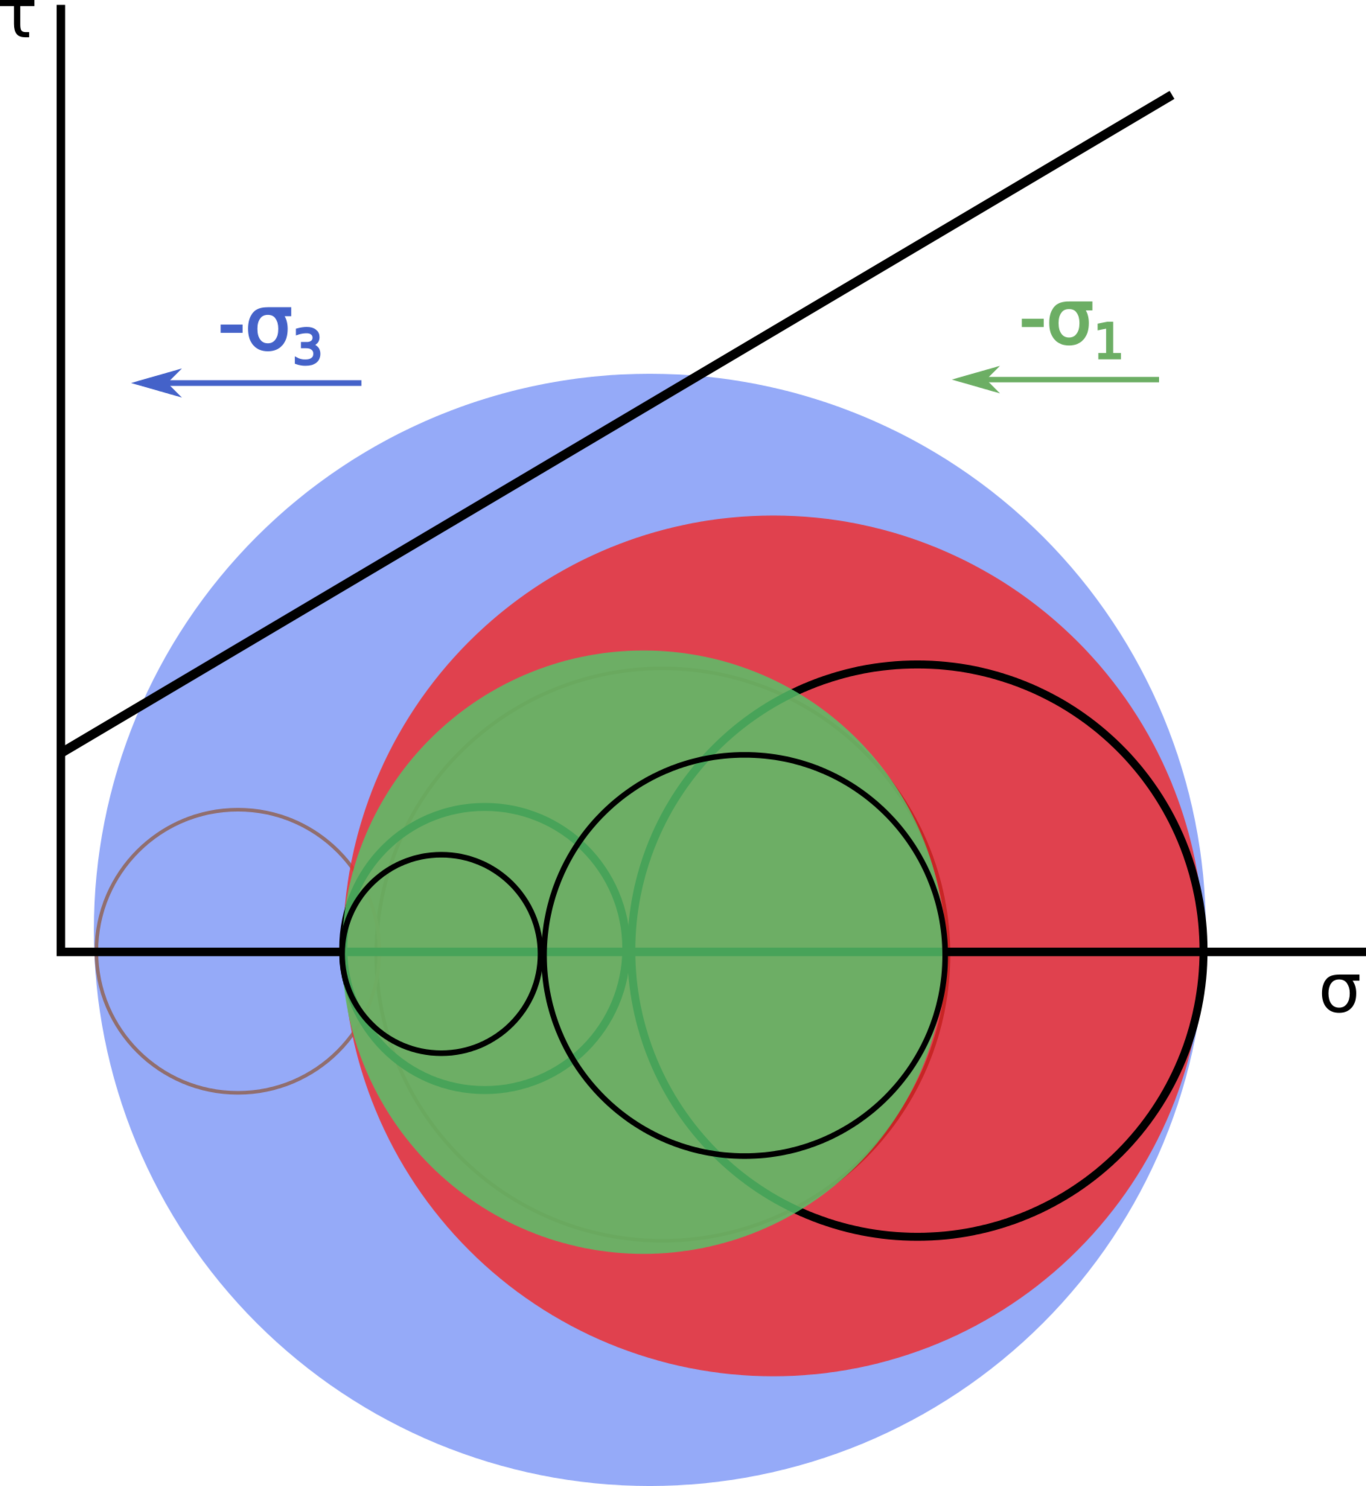
\includegraphics[width=0.7\columnwidth]{Chapter_1_Intro/figures/T_decrease_mohr/T_decrease_mohr}
\caption[Mohr's circles showing the effect of thermo-elastic stress reduction]{{
Schematic illustration of the changes in the Mohr's circle induced by
thermoelastic stress changes in a reservoir due to the injection of cold
fluid. The red circle represents the undisturbed state. The
induced change in the reservoir stress state is dependent upon the
shape of the cooled zone as it relates to the directions of the principal
stress axes. Cooling preferentially decreases the magnitude of stress
parallel to the dominant direction of flow (and hence the longest axis of the cooled zone) \citep{Jeanne_2014}. The blue circle illustrates the effect of fluid flow parallel
to $\sigma_{3}$, which would increase the differential stress (defining the diameter of the blue circle) and bring the fracture network closer to a critical stress state. If
fluid flow is parallel to $\sigma_{1}$, then differential stress
is decreased and the fracture network is made more stable. In the
normal-faulting stress state of the \acrshort{TVZ} ($\sigma_{1}\approx{\sigma_{V}}$), the blue circle would correspond to a preferred NW-SE flow
direction, whereas NE-SW flow would reduce $\sigma_2$, a state
which would be represented by a Mohr's circle equal in size to the red
circle, but with modified sizes of the subcircles. This would signify a
change in the orientation of fractures which would be able to fail.
{\label{621452}}%
}}
\end{center}
\end{figure}

\subsection{Permeability and Seismicity}
For most industrial applications of fluid injection, formation permeability is of paramount importance. Generally, fluid injection operations either seek to increase permeability (e.g. geothermal well stimulation, hydraulic fracturing) or require that sufficient permeability exists so that the formation will accept the fluid being injected (e.g. wastewater disposal, CO$_2$ sequestration, enhanced oil recovery) \citep{2013}. Induced seismicity, as it relates to any given injection, can be viewed in two lights: as a risk to be mitigated, or as a tool for tracking changes in the reservoir. When viewing IS as a potential risk, it must be weighed against the goals of the project, which often include increasing the formation permeability (e.g. fracking or geothermal stimulation). In these cases, operators must ask how much permeability gain is enough, and what level of seismicity is too much. At the same time, if IS is to be used as a monitoring tool (for instance, to map the stimulated volume of rock during an EGS project), operators need to know what information it provides. If the occurrence of seismicity implies a perturbation of pore-fluid pressure or reservoir stress change, does it also imply change in permeability? In order to satisfactorily answer these questions, the relationship between seismicity and reservoir permeability must be better understood.

The seismicity-permeability relationship has been widely studied in laboratory settings for a number of years \citep[e.g.][and citations therein]{Lee_2002}. Generally, when slip occurs on a preexisting fracture, the permeability of that fracture also increases through a process known as self-propping, where the misalignment of asperities on opposing fracture walls leads to an increase in fracture aperture, and thus permeability (Figure \ref{363218}). The degree to which fracture permeability is affected by slip depends on the length of the slip vector, rupture velocity, the roughness of the fracture surface and the material within the fracture (gouge) \citep{Fang_2017}. Fracture permeability can also increase as a result of displacement normal to the fracture plane through processes such as thermal contraction of the fracture walls or pore pressure increase (Figure \ref{363218}).

\citet{Guglielmi_2015} and \citet{cappa2019stabilization} measured shear and normal displacement during injection into a decameter-scale fault and found that fault permeability was most sensitive to normal displacements early in the injection, with relatively little permeability gain related to shear displacements induced at later stages of the injection. This result questions the commonly-held belief that the stimulation (i.e. permeability increase) of injection wells at sub-$\sigma_{3}$ pressures, is due to induced shear on hydraulically-connected fractures. Instead, permeability increase could be largely due to normal displacements that are aseismic due to possible rate-strengthening behavior induced by fluid injection. In turn, this calls into question the use of seismicity as a way to map the extent of the stimulated reservoir \citep[e.g.][]{Fang_2018,Yoon_2014,Dempsey_2015}. This permeability-seismicity decoupling was recently illustrated through modeling of the Habanero and Paralana EGS project in Australia \citep{Riffault_2018}.

Aseismic motions are important contributors to permeability change in isothermal environments, such as shallow mines \citep{Guglielmi_2015}, or shale reservoirs \citep{Das_2011}. However, they may play an even more important role in high-temperature geothermal environments where thermoelastic contraction of fracture walls may serve to encourage fracture normal displacement. A model where well permeable zones expand and contract in response to thermal stresses is widely accepted at geothermal fields in New Zealand, where it has been used to describe oscillating \gls{injectivity} behavior in response to injection-related cooling, and subsequent heating in the absence of injection \citep{grant2013thermal}.

A final, and more difficult to characterize, factor influencing reservoir permeability is fluid chemistry. As fluid moves through a formation, it may dissolve minerals out of, or precipitate minerals into, fractures, depending on the pressure and temperature and composition of the fluid. Though less well-understood, this effect probably plays a large part in creating or destroying permeability through opening or sealing of fractures that would be likely to fail \citep{Clearwater_2015}. In this work, we will not address this issue, but it must be noted as a significant source of uncertainty with respect to reservoir permeability.\selectlanguage{english}

\begin{figure}[h!]
\begin{center}
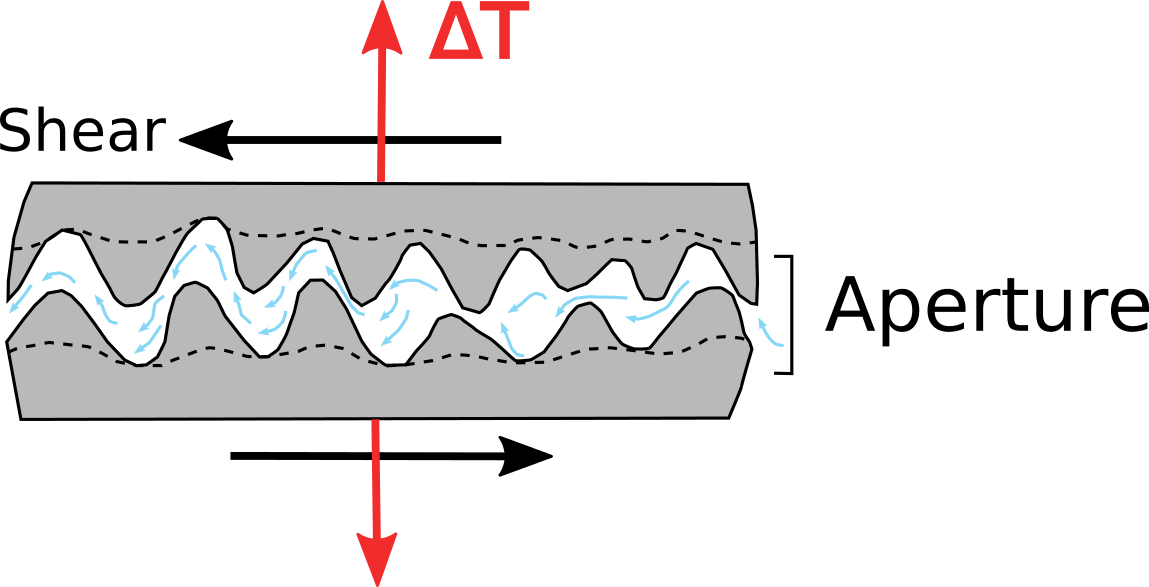
\includegraphics[width=0.70\columnwidth]{Chapter_1_Intro/figures/simple_stim_fig/simple_stim_fig}
\caption[Cartoon of fracture permeability increase]{{
Simple schematic (adapted from \protect\citet{Fang_2017}) illustrating the
possible fracture aperture increase associated with slip on a fault, fracture opening (due to pressure increase or thermal contraction of the fracture walls), or some combination of both.
{\label{363218}}%
}}
\end{center}
\end{figure}

\section{Study Aims}
The primary goal of this thesis is to establish quantifiable relationships between the occurrence of seismicity and power production operations, specifically fluid extraction and injection, at the Rotokawa and Ngatamariki geothermal fields. The specific research questions that we will address are as follows:

\begin{enumerate}
  \item{How do variations in the rate, location and magnitude of seismicity at each field relate to the injection and withdrawal of fluid?}
  \item{Can a relationship be established between well stimulation (i.e. \gls{permeability} increase) and seismicity?}
  \item{Do earthquake focal mechanisms aid in characterizing the orientation and extent of the reservoir fracture network?}
  \item{What can spatial and temporal variations in stress state tell us about injection and production-related changes to the reservoir?}
\end{enumerate}

In order to answer these questions, we will construct a comprehensive catalog of seismicity for both fields. This process will include the completion of the following tasks:
\begin{itemize}
  \item{Compile an automatically-detected catalog of seismicity (Question 1, Chapter 2);}
  \item{Detect additional, smaller-magnitude events using the automatically-detected events as templates ing a matched-filter routine \citep{Chamberlain_2017} (Question 1--2, Chapters 2--4);}
  \item{Relocate the entire catalog using a non-linear, grid search algorithm \citep{Lomax_2014}, with locations further refined by a relative-relocation algorithm \citep{Trugman_2017} (Question 1--2, Chapters 2--5);}
  \item{Implement a magnitude estimation methodology \citep{Shelly_2016} for events detected using the matched-filter technique (Question 1-2, Chapters 2--4);}
  \item{Manually pick P-wave first arrival polarities and invert for focal mechanism solutions \cite{Walsh_2009} (Question 3--4, Chapter 5);}
\end{itemize}

The analysis of this catalog as it relates to the injection and production operations at the fields will involve the following additional step:
\begin{itemize}
  \item{Invert focal mechanism solutions for stress state over time and space \citep{Arnold_2007,Lund_2007} (Question 4, Chapter 5);}
\end{itemize}

The research presented here is funded by Mercury NZ Ltd., who have identified several periods of interest in which the reservoir behaved in unexpected or interesting ways. We will focus on addressing each of these periods in turn and relate the characteristics of seismicity within the reservoir to the parameters measured at the wells in question. The periods of interest are summarized in Table \ref{table:objectives}.\selectlanguage{english}

\begin{table}
\begin{tabular}{cccc}
    {Field} & {Operation} & {Start} & {End}\\ \midrule
    Ngatamariki & NM08 stimulation & June-2012 & July-2012\\
    Ngatamariki & NM09 stimulation & December-2012 & January-2013\\
    Ngatamariki & NM10 drilling losses & July-2012 & August-2012\\
    Ngatamariki & NM12 drilling losses  & June-2014 & September-2014\\
    Rotokawa & RK24 \gls{injectivity} decline & 2012 & 2013\\
    Rotokawa & Injection switch: RK24-RK23 & June-2014 & July-2014\\
    Rotokawa & RK34 drilling losses & September-2014 & November-2014\\
    Rotokawa & Plant maintenance & 2012-2015 & 2012-2015\\
\end{tabular}
\caption[Periods of interest addressed in this thesis]{{
Table summarizing the key periods of interest specified by Mercury for the years 2012-2015. These periods define the focus of study for comparing
changes in well parameters to the response in seismicity.}}
\label{table:objectives}
\end{table}

\section{Thesis structure}
Chapter 2, following this introductory chapter, will discuss in detail the seismic data and network that provide the raw basis for this work. It will also touch on the supplemental, borehole data gathered by Mercury NZ, Ltd and explain the basic methods used to detect, locate, determine magnitudes and calculate focal mechanisms for seismic events.

Chapters 3, 4 and 5 contain distinct, standalone projects and have been written and formatted with the intent of publication.

Chapter 3 has been submitted to G-cubed as a manuscript entitled, "Seismic Response to Injection Well Stimulation in a High-Temperature, High-Permeability Reservoir" and addresses the relationship between seismicity and injection during the stimulation and completion tests undertaken prior to the startup of the Ngatamariki power plant. Coauthor Stefan Mroczek contributed automatic S-picks to the catalog presented in this and all other chapters. A more detailed methodology for this process is described in \citet{mroczek2016shear}. In addition, coauthor Steven Sewell contributed geologic context and interpretation of these results.

Chapter 4 parallels Chapter 3, but at Rotokawa. It relates the rate, location and magnitude of seismicity to changes in injection from 2012--2016. It also attempts to establish relationships between the frequency-magnitude distribution of Rotokawa seismicity and the reservoir pressure distribution.

Chapter 5 details the spatial and temporal variations in focal mechanisms, magnitudes and stress at both Ngatamariki and Rotokawa between 2012 and 2015.

Finally, chapter 6 summarizes the findings of the preceding three chapters and suggests potential paths along which the research presented here could continue.

Chapters 3, 4 and 5 each contain detailed descriptions of the methodologies used. Therefore, chapter 2 will address only the methods used in creating the underlying earthquake catalog, which includes linearized, grid-search and double difference earthquake locations, event magnitudes and event focal mechanisms. All further explanation of the more complex methods applied in the standalone chapters will therefore be addressed in the appropriate chapter.

The vast majority of the work presented in this thesis was conducted by me (Chet Hopp). However, I have chosen to write this thesis in the first-person plural, as is consistent with, and in acknowledgment of, the significant contributions of both my supervisors and colleagues, who have been included in chapter 3 as authors of the submitted manuscript. To this point, the initial, amplitude-based detection and linear location of the earthquake catalog from which this work began was conducted by a team of researchers at GNS Science in Wairakei and elsewhere, under contract with Mercury NZ, Ltd. This contribution was instrumental in directing the rest of this research and, because of this, deserves mentioning here.
% 	\cleardoublepage
% 	\chapter{Data and Methods}
Much of this thesis relies on the analysis of earthquake catalogs which, along with raw waveforms, are the basis of seismology. A number of methods are used in this thesis, both by me and by colleagues and supervisors, in order to derive a catalog of seismicity from raw, unfiltered waveforms recorded at a seismograph stations. This chapter aims to describe the steps taken to create the earthquake catalog analyzed in each of the subsequent chapters. At its most basic, our earthquake catalog for Rotokawa and Ngatamariki contains information about the time of occurrence, location of the event, magnitude of the event and, in some cases, information about how the fault or fracture slipped (focal mechanisms). What follows is a description of the methods of detection, location, magnitude estimation and focal mechanism determination starting from raw waveforms.

Apart from seismic data, a number of other data streams are used in this thesis for the purpose of assessing the relationship between seismicity and geothermal field operations. These data are touched upon in Chapter 1, but those with the greatest significance to this work will be detailed here. Specifically, well pressure, temperature and \gls{flow_rate} measurements are used extensively both for direct comparison to rates of seismicity and also to make inferences about the reservoir. 

\section{Data}
\subsection{Seismic network}
The seismic data presented in this thesis were recorded on a network of between 15 and 29 seismometers, most of which are concentrated in an area 15 km N-S by 7 km E-W centered around the Rotokawa and Ngatamariki geothermal fields (Figures \ref{322599} and \ref{continuity}). The vast majority of the stations are owned and operated by Mercury NZ Ltd., for the purpose of monitoring the geothermal fields. However, six stations from either Contact Energy (ARAZ, THQ2) or GeoNet, the national seismic network (HRRZ, PRRZ, ALRZ, WPRZ), have been incorporated into this network to improve station coverage.

GNS Science in Waikarei has been contracted to maintain the seismic network at the geothermal fields, a task which includes quarterly retrieval of data, which is stored locally at each station between servicing trips. As detailed in Table \ref{station_table}, the Mercury-operated stations are 4.5 Hz geophones and the data are sampled at 200 Hz. Three of these stations are borehole instruments (NS12, NS13, NS14), deployed in the center of the Ngatamariki field at depths of between 202 and 514 m. The GeoNet data are sampled at 100 Hz and were downloaded and archived locally at the outset of this project in order to speed up analysis.

As the Rotokawa reservoir has been developed for considerably longer than Ngatamariki, its seismic network (stations named RT) has been in operation for over a decade. Ngatamariki stations began to be installed prior to drilling operations in mid-2012. Network coverage varied with time as certain stations were moved to improve performance or replaced after damage due to livestock or vandalism (Figure \ref{continuity}). Therefore, the network presented in Figure \ref{322599} does not represent the exact geometry for any specific point in time, instead reflecting the locations of instruments that were operational at any point between 2012 and 2015.\selectlanguage{english}

\begin{figure}[h!]
\begin{center}
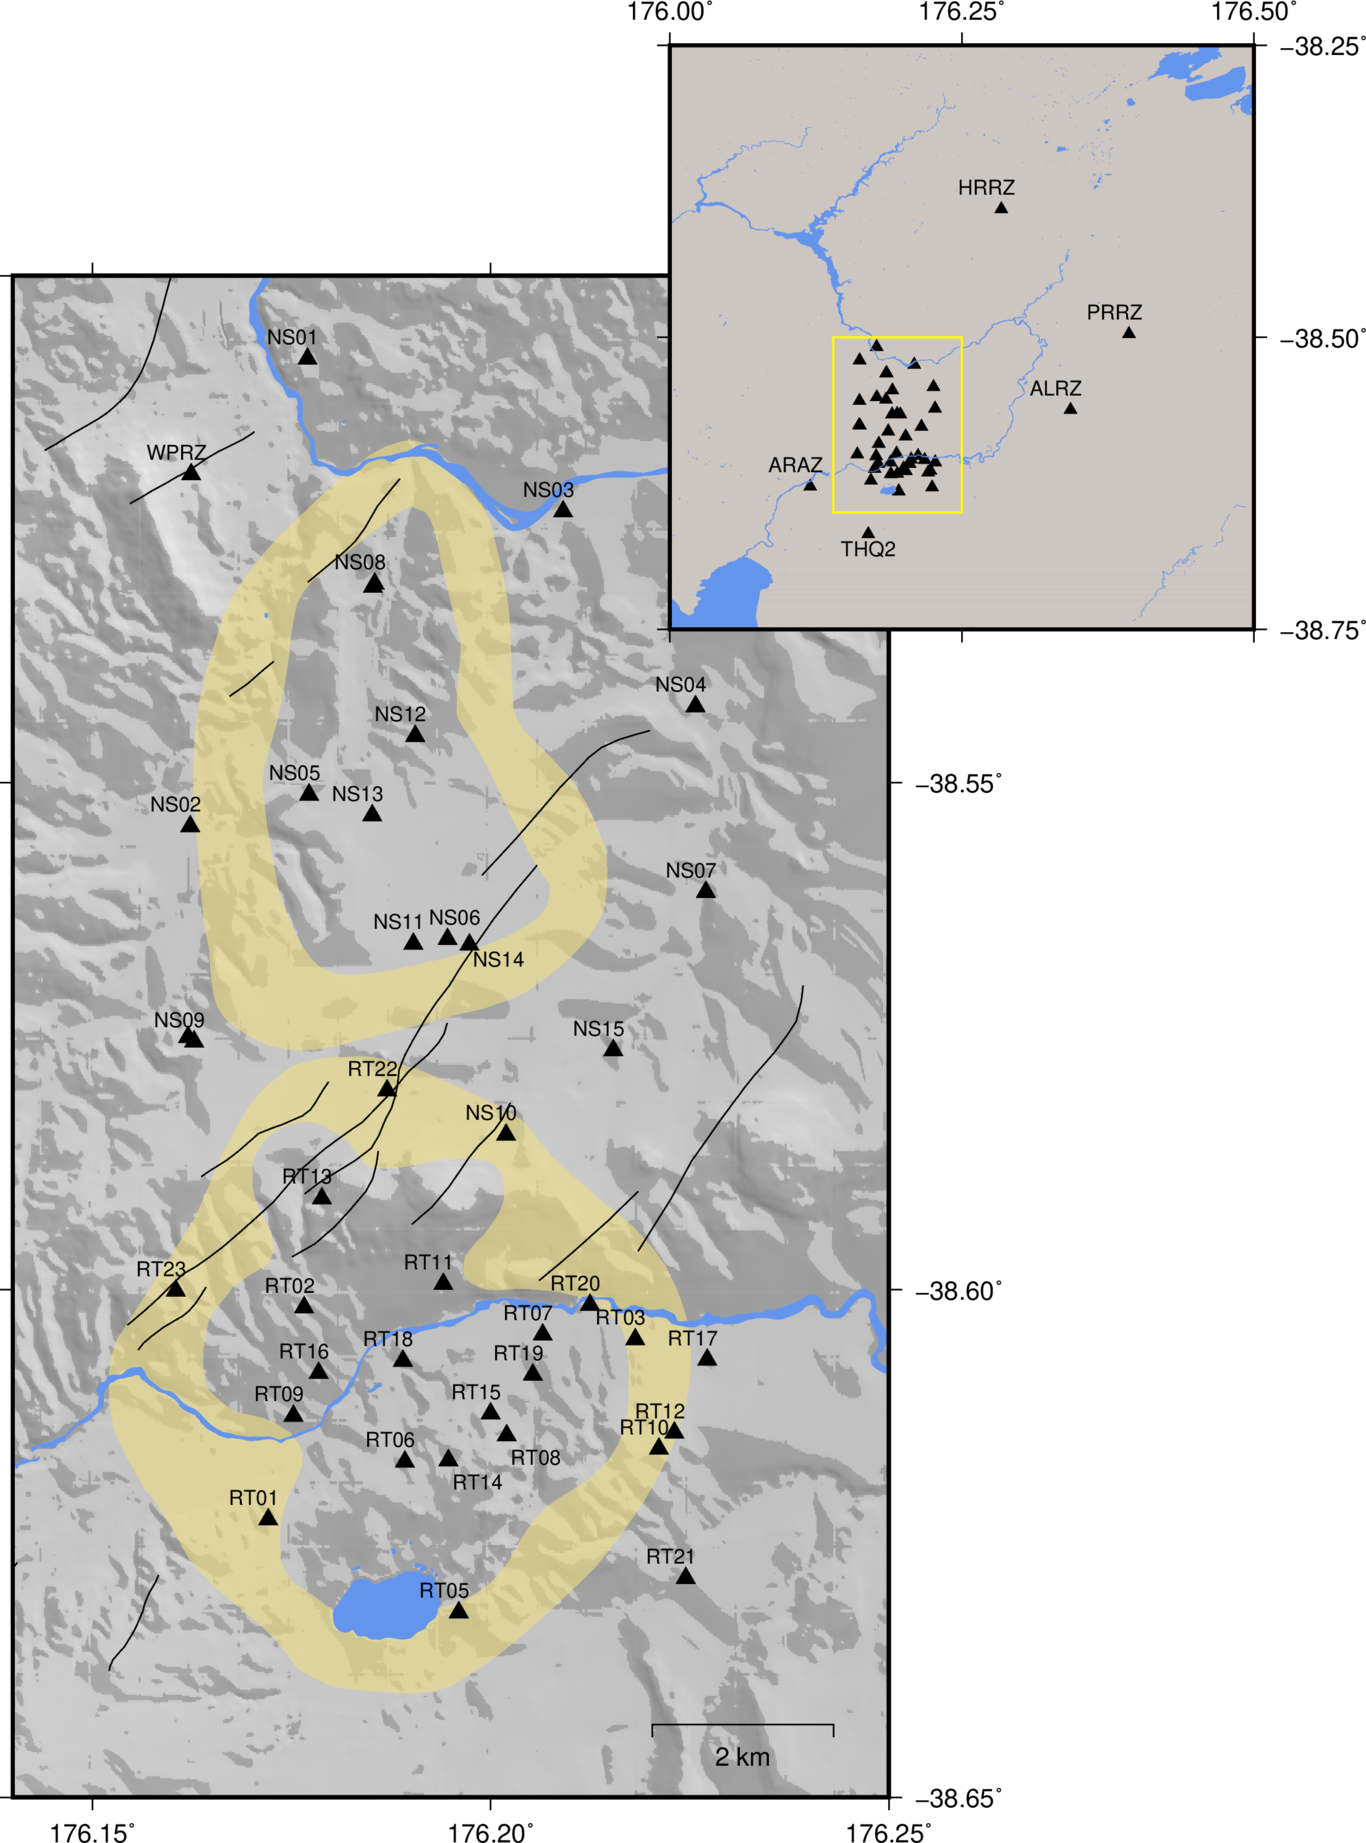
\includegraphics[width=0.70\columnwidth]{Chapter_2_Data/figures/RotNga_stations_overview/RotNga_stations_overview}
\caption[Seismograph station map]{{
All stations that were active at any time between 2012 and 2015.
Goldenrod shapes indicate the most likely resistivity boundaries for the
Ngatamariki and Rotokawa geothermal fields, triangles show the locations
of seismic stations, each of which is labeled with the station name
appearing in Table 1, below.
{\label{322599}}%
}}
\end{center}
\end{figure}\selectlanguage{english}

\begin{table}
\centering
\resizebox{\textwidth}{!}{%
\begin{tabular}{cccccc}
    {Station name} & {Longitude} & {Latitude} & {Elevation (m)} & {Depth (m)} & {Sensor} \\ \midrule
    ALRZ & 176.343014 & -38.562043 & 405.0 & 0.0 & L4C-3D \\
    ARAZ & 176.12006 & -38.62769 & 420.0 & 0.0 & L4C-3D \\
    HRRZ & 176.283754 & -38.39013 & 590.0 & 0.0 & L4C-3D \\
    NS01 & 176.177 & -38.5082 & 349.0 & 0.0 & Geospace GS-11D \\
    NS02 & 176.162275 & -38.554318 & 375.0 & 0.0 & Geospace GS-11D \\
    NS03 & 176.209102 & -38.523259 & 327.0 & 0.0 & Geospace GS-11D \\
    NS04 & 176.225718 & -38.542487 & 345.0 & 0.0 & Geospace GS-11D \\
    NS05 & 176.1772 & -38.5512 & 386.0 & 0.0 & Geospace GS-11D \\
    NS06 & 176.194571 & -38.565449 & 407.0 & 0.0 & Geospace GS-11D \\
    NS07 & 176.227019 & -38.560793 & 345.0 & 0.0 & Geospace GS-11D \\
    NS08 & 176.185438 & -38.530393 & 345.0 & 0.0 & Geospace GS-11D \\
    NS09 & 176.162759 & -38.575539 & 451.0 & 0.0 & Geospace GS-11D \\
    NS10 & 176.201928 & -38.584723 & 400.0 & 0.0 & Geospace GS-11D \\
    NS11 & 176.1903 & -38.5659 & 409.0 & 0.0 & Geospace GS-11D \\
    NS12 & 176.190524 & -38.545408 & 350.0 & 514.0 & IESE Borehole: Duke 4.5 \\
    NS13 & 176.185137 & -38.553235 & 380.0 & 250.0 & IESE Borehole: Duke 4.5 \\
    NS14 & 176.197332 & -38.565986 & 365.0 & 202.0 & IESE Borehole: Duke 4.5 \\
    NS15 & 176.2154 & -38.5764 & 382.0 & 0.0 & Geospace GS-11D \\
    NS16 & 176.162 & -38.5751 & 450.0 & 0.0 & Geospace GS-11D \\
    NS18 & 176.1852 & -38.5307 & 348.0 & 0.0 & Geospace GS-11D \\
    PRRZ & 176.393 & -38.4971 & 392.0 & 0.0 & L4C-3D \\
    RT01 & 176.17208 & -38.62264 & 371.0 & 0.0 & LE-3Dlite \\
    RT02 & 176.17658 & -38.60173 & 346.0 & 0.0 & LE-3Dlite \\
    RT03 & 176.21815 & -38.60488 & 337.0 & 0.0 & LE-3Dlite \\
    RT05 & 176.19599 & -38.63178 & 369.0 & 0.0 & LE-3Dlite \\
    RT06 & 176.18922 & -38.61694 & 366.0 & 0.0 & LE-3Dlite \\
    RT07 & 176.20653 & -38.60443 & 320.0 & 0.0 & LE-3Dlite \\
    RT08 & 176.20201 & -38.61436 & 341.0 & 0.0 & LE-3Dlite \\
    RT09 & 176.17524 & -38.61243 & 339.0 & 0.0 & Geospace GS-11D \\
    RT10 & 176.22112 & -38.61567 & 408.0 & 0.0 & Geospace GS-11D \\
    RT11 & 176.194057 & -38.599442 & 330.0 & 0.0 & Geospace GS-11D \\
    RT12 & 176.223066 & -38.614089 & 400.0 & 0.0 & Geospace GS-11D \\
    RT13 & 176.1788 & -38.591 & 428.0 & 0.0 & Geospace GS-11D \\
    RT14 & 176.1947 & -38.6168 & 380.0 & 0.0 & Geospace GS-11D \\
    RT15 & 176.2 & -38.6122 & 352.0 & 0.0 & Geospace GS-11D \\
    RT16 & 176.1784 & -38.6082 & 336.0 & 0.0 & Geospace GS-11D \\
    RT17 & 176.2272 & -38.6069 & 342.0 & 0.0 & Geospace GS-11D \\
    RT18 & 176.188968 & -38.606998 & 308.0 & 0.0 & Geospace GS-11D \\
    RT19 & 176.205294 & -38.608375 & 312.0 & 0.0 & Geospace GS-11D \\
    RT20 & 176.212467 & -38.601494 & 300.0 & 0.0 & Geospace GS-11D \\
    RT21 & 176.2245 & -38.6284 & 250.0 & 0.0 & Geospace GS-11D \\
    RT22 & 176.186985 & -38.580367 & 423.0 & 0.0 & Geospace GS-11D \\
    RT23 & 176.160466 & -38.600085 & 447.0 & 0.0 & Geospace GS-11D \\
    THQ2 & 176.1698 & -38.6684 & 450.0 & 80.0 & IESE Borehole: Duke 4.5 \\
    WPRZ & 176.1624 & -38.5196 & 519.0 & 0.0 & LE-3DliteMkII \\
\end{tabular}}
\caption[Seismograph station information]{{
Summary of each station active at any time between 2012 and 2015 at Rotokawa and Ngatamariki. Most stations are owned and operated by Mercury NZ Ltd. However, stations ARAZ and THQ2 are owned and operated by Contact Energy and stations ALRZ, HRRZ, PRRZ and WPRZ are operated by the national seismic network, GeoNet.}}
\label{station_table}
\end{table}

\begin{figure}[h!]
\begin{center}
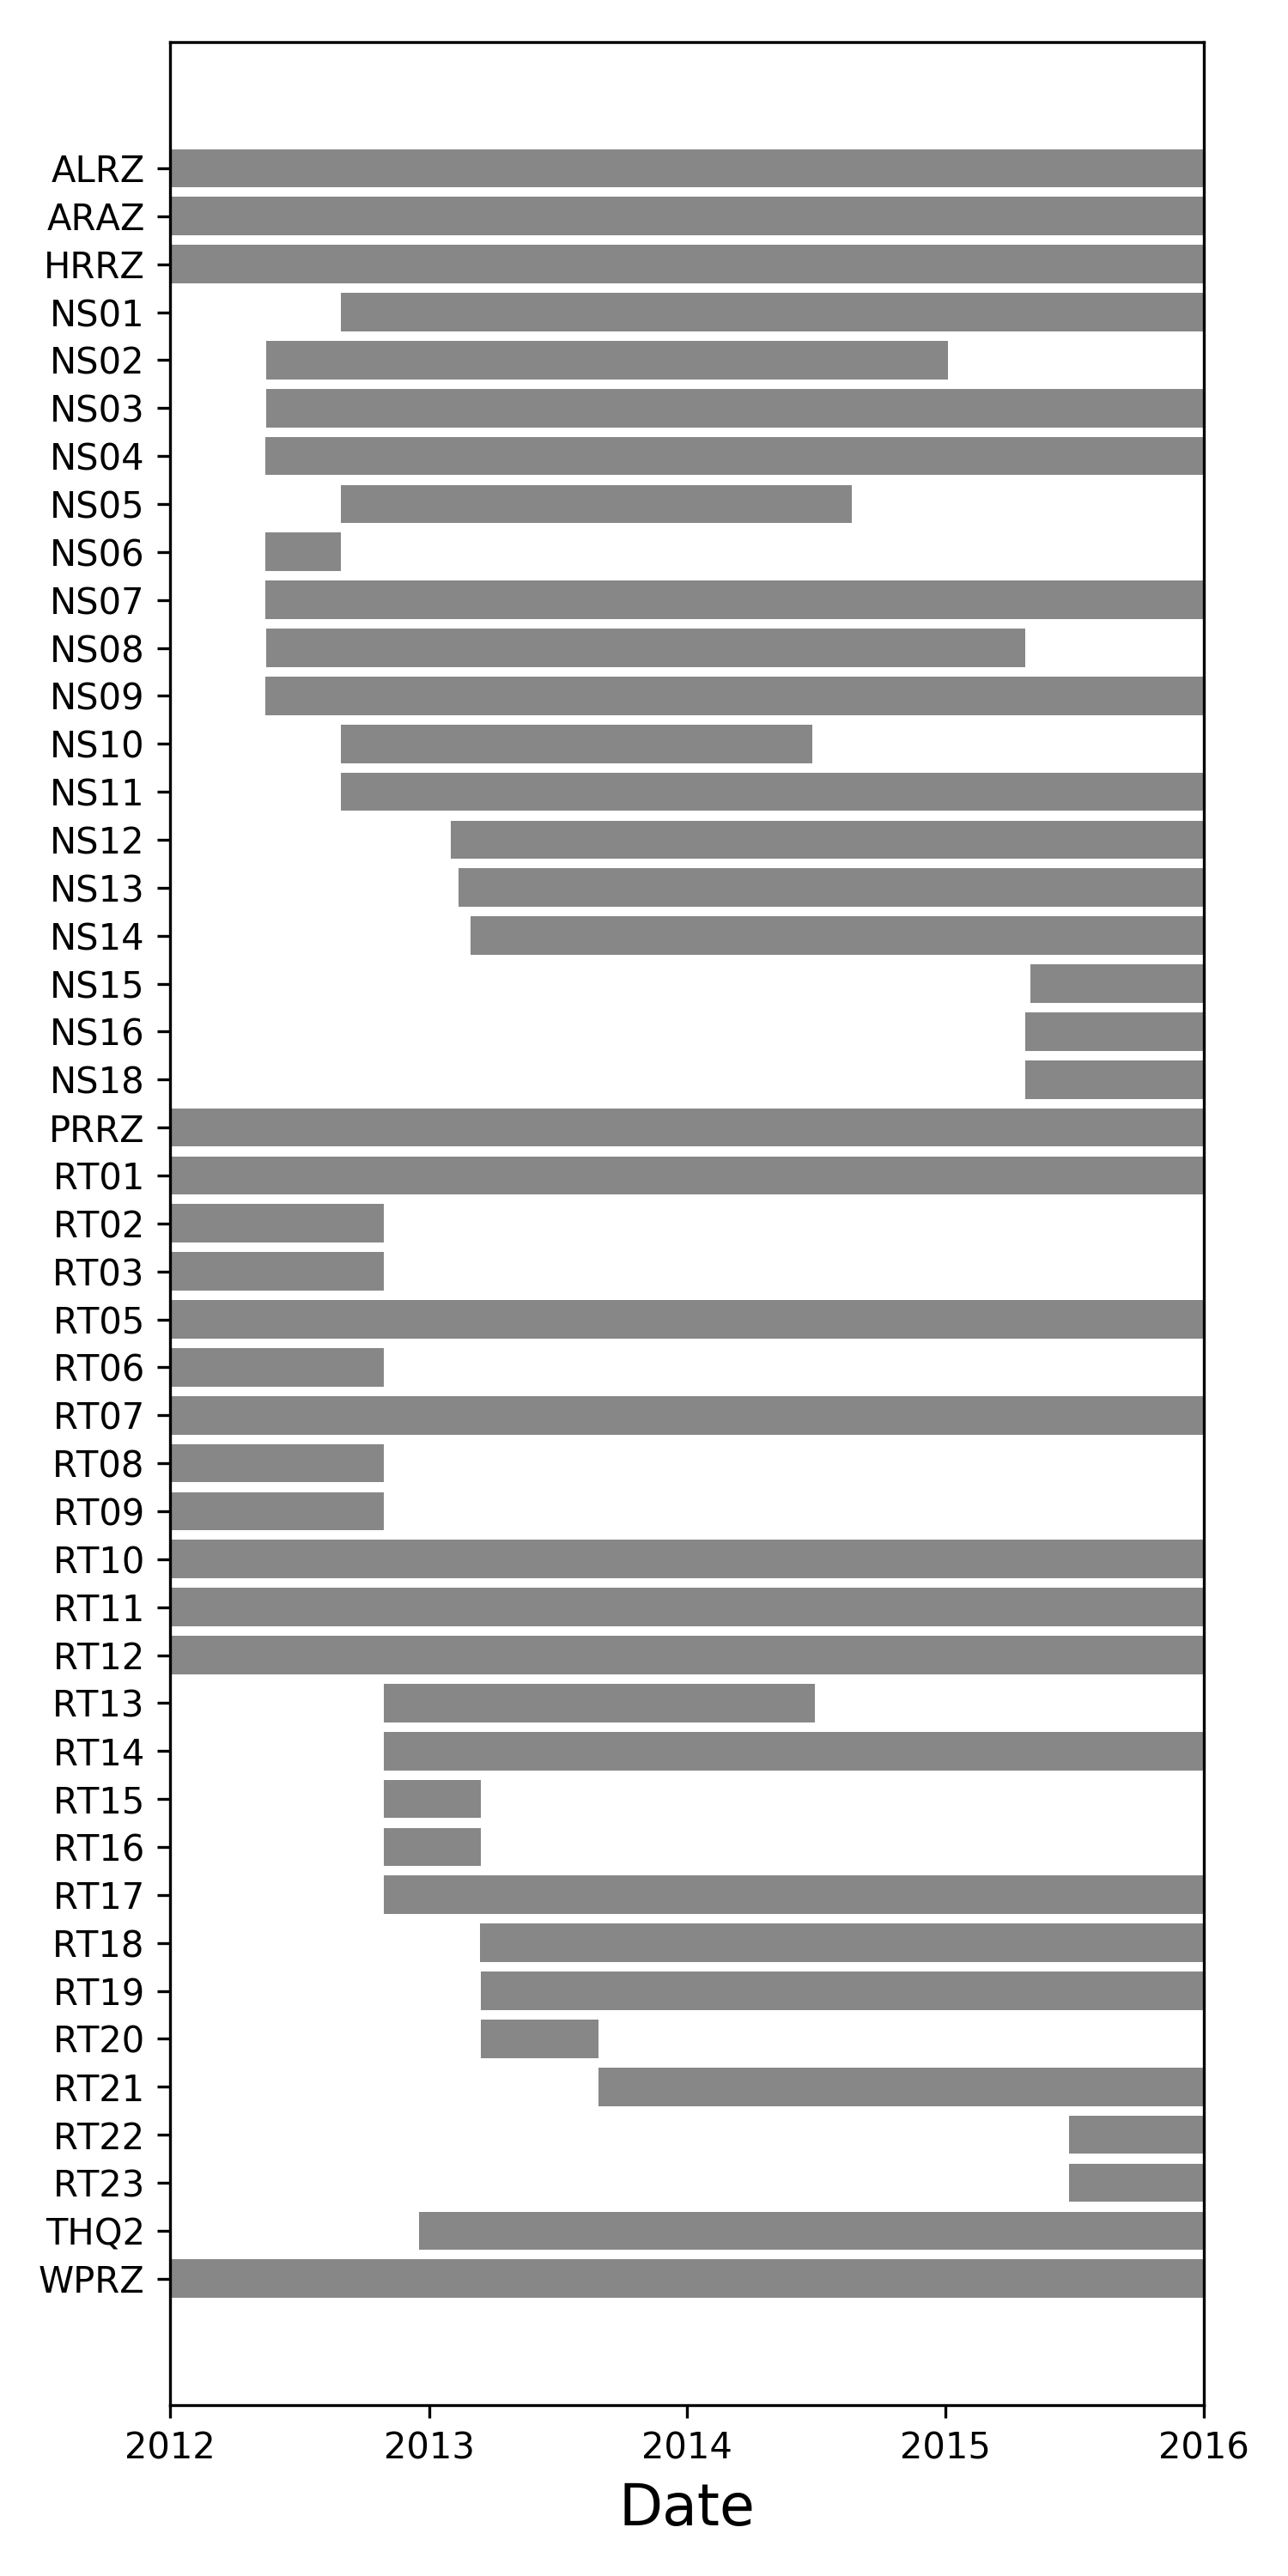
\includegraphics[width=0.70\columnwidth]{Chapter_2_Data/figures/data_continuity/Mercury_data_continuity_3-13}
\caption[Data continuity]{{
Data continuity plot for the seismic network detailed in Figure \ref{322599} and Table \ref{station_table}. Gray lines show the period during which each station was operational.
{\label{continuity}}%
}}
\end{center}
\end{figure}\selectlanguage{english}

\subsection{Preliminary earthquake catalog}\label{GNS_cat}
As stated above, the initial earthquake catalog was constructed by GNS Science using the software package SeisComP3 \citep{Weber2007}. Event detection was done using a short-term average\slash{long-term average} technique, which records a detection when the ratio of the average amplitude in a user-defined, short-term window to that in a long-term window exceeds a threshold value. Each of these detections was then automatically located using the linearized location algorithm Hypo71 \citep{Lee_1972}. See Sections \ref{STA/LTA} and \ref{linloc} for a detailed description of these techniques.

Local magnitudes were also calculated using the SeisComP3 module \textit{scmag}, which uses the ubiquitous equation from Richter \citep{richter1935instrumental} for magnitude at an individual station:

\begin{equation}
M_L = \log_{10}{A} - \log_{10}A0
\end{equation}

where $A$ is the amplitude of the seismic trace in mm and $A0$ is a calibration term that is used to adjust the scale to different localities. In this case, the SeisComP3 \textit{logA0} module was used with distance calibration values of $A0$ summarized in Table \ref{table_A0}. The magnitudes at each station were averaged to return the final event magnitude.\selectlanguage{english}
\begin{table}
\centering
\begin{tabular}{cc}
    {Event-station dist (km)} & {Calibration A0 (mag. units)} \\ \midrule
    0  & 0.0431 \\
    10  & -1.1563  \\
    50  & -1.5755  \\
    100  & -1.7560  \\
    1000  & -2.3545   \\
\end{tabular}
\caption[Magnitude calculation distance correction factors]{{
Table summarizing the distance correction factors used by GNS Science in calculating the magnitudes of the preliminary earthquake catalog.}}
\label{table_A0}
\end{table}

The national seismic network, GeoNet, reports location and magnitude information for most earthquakes above magnitude 2.1 in the area of Rotokawa and Ngatamariki \citep{Sherburn_2015}. The GeoNet-calculated magnitudes of such events at the geothermal fields were compared with the independently-calculated magnitudes from the stations in the Mercury network used in this study (note that three stations from the GeoNet network were included in the Mercury seismic network). There was found to be a disagreement between GeoNet- and Mercury-calculated magnitudes of -0.32 magnitude units, which was addressed by applying a static correction of +0.32 to all Mercury-network magnitudes in the preliminary catalog used in this thesis. The corrected magnitudes are compared to the GeoNet magnitudes in Figure \ref{910533}, showing that the relationship between the two sets of magnitudes is approximately 1:1.\selectlanguage{english}

\begin{figure}[h!]
\begin{center}
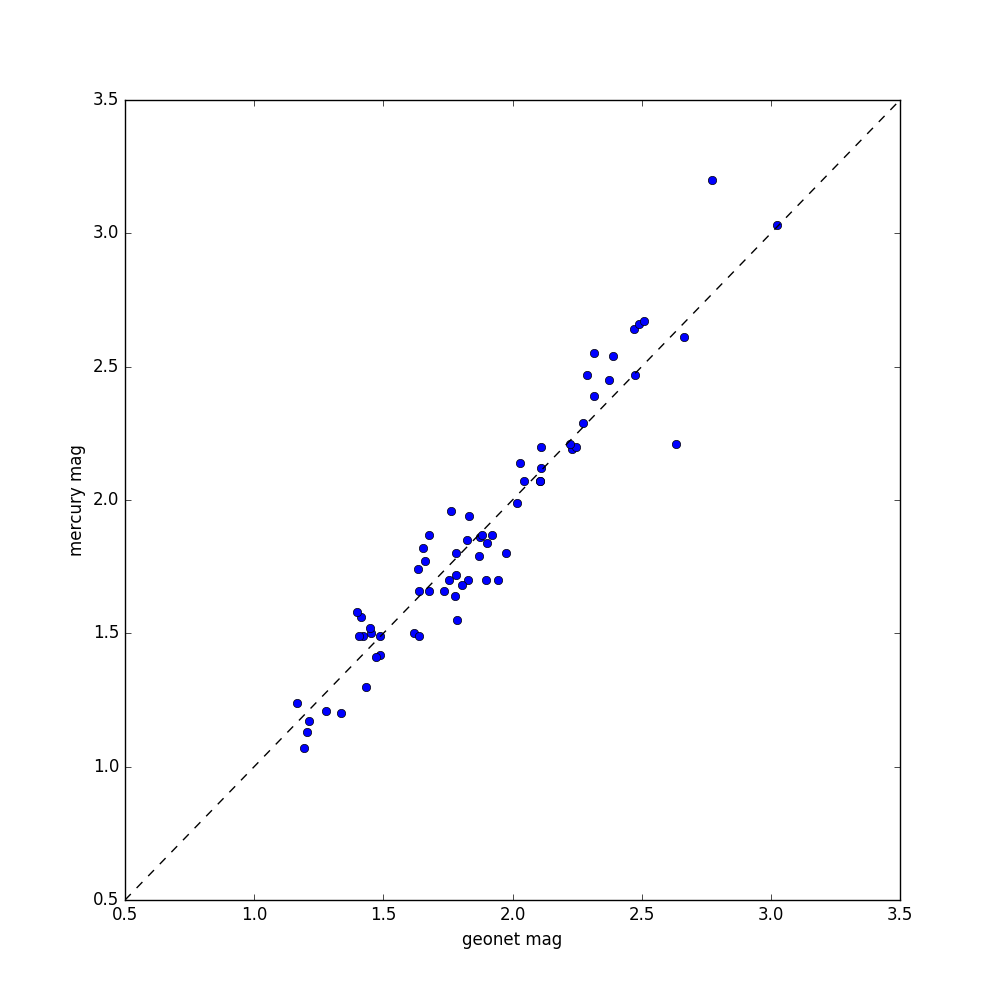
\includegraphics[width=0.70\columnwidth]{Chapter_2_Data/figures/geonet-merc_mag_comp/geonet-merc_mag_comp}
\caption[Mercury vs. GeoNet magnitude relationship]{{
Mercury-calculated vs GeoNet calculated magnitudes after applying a
static correction of +0.32 magnitude units to the Mercury events.
{\label{910533}}%
}}
\end{center}
\end{figure}

Following the steps outlined above, GNS Science provided us the Rotokawa\slash{Ngatamariki} earthquake catalog in the form of \textit{SeisComP3} native \textit{sc3ml} xml files. This catalog contained 8226 earthquakes that occurred between 15 May 2012 and 18 November 2015 (black events, Figure \ref{955268}). These two dates correspond to the date of the start of the first Ngatamariki seismographs, at which time the Rotokawa and Ngatamariki seismic networks were combined, and the final data-collection date of 2015, respectively. Many of these events occurred outside of the boundaries of the geothermal fields and were therefore marginally applicable to the aims of this thesis. For this reason, we filtered the catalog to include only events that occurred within or adjacent to the field boundaries of Rotokawa and Ngatamariki, and also to include events with average pick residuals within one standard deviation of the mean, leaving a total of 4405 events (Figure \ref{955268}). These earthquakes were used as 'template' events in detecting additional events as detailed in Section \ref{MF} below.\selectlanguage{english}

\begin{figure}[h!]
\begin{center}
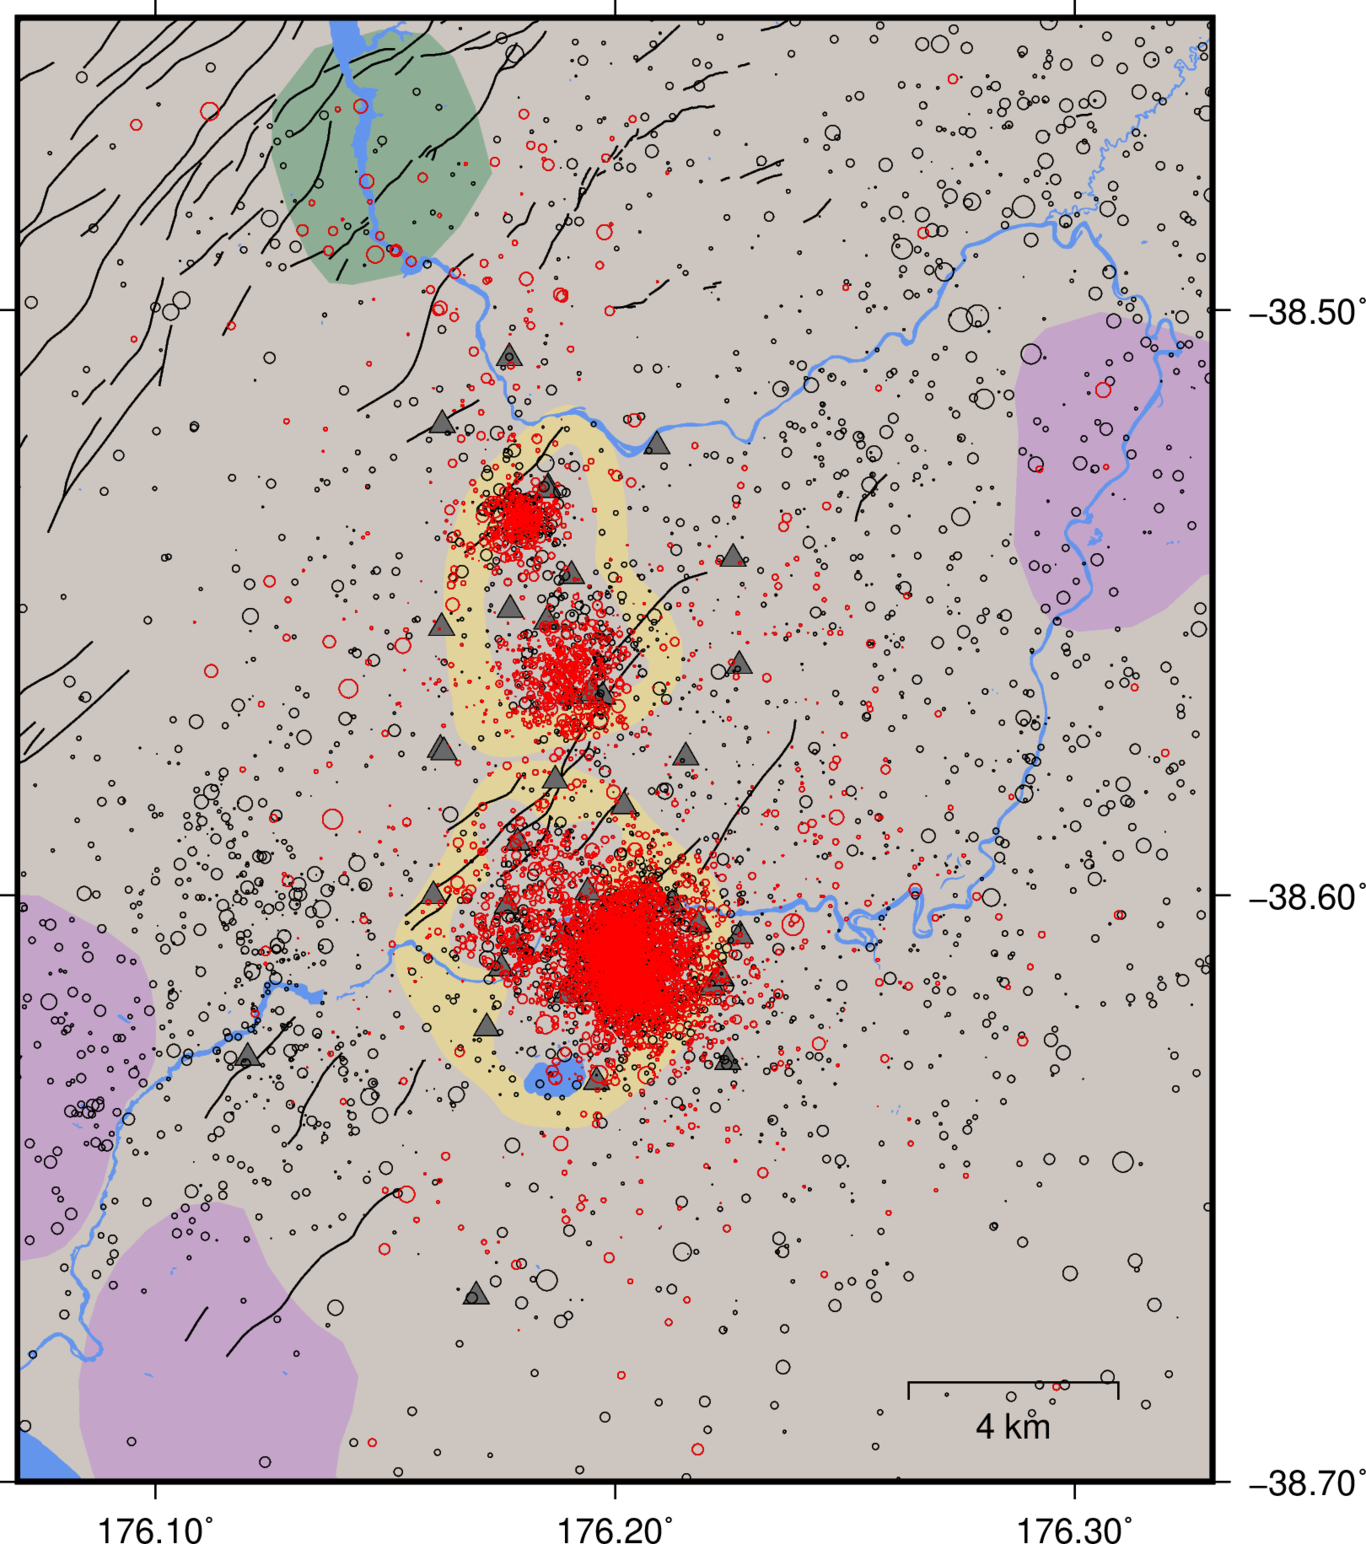
\includegraphics[width=0.70\columnwidth]{Chapter_2_Data/figures/RotNga_catalog_overview/RotNga_catalog_overview}
\caption[GNS template event locations]{{
Overview of earthquakes in the preliminary GNS Science catalog. Red
events are those which were selected for use in the analyses detailed in
the following sections. Gray triangles represent seismograph stations.
Yellow indicates the boundaries of the Ngatamariki and Rotokawa
geothermal fields, purple nearby Contact Energy-operated fields, and
green the protected Orakei-Korako geothermal field. Black lines show
active faults \citep{AFDB}. Event symbols are scaled by magnitude where the largest
is magnitude 4.2.
{\label{955268}}%
}}
\end{center}
\end{figure}

\subsection{Mercury datasets}
In this thesis, we make use of a number of additional datasets that have been provided by Mercury. These data record the industrial processes taking place at the fields (such as injection and extraction of fluids) as well as properties of the deep reservoir that can be directly measured or inferred from the limited number of wells. They also provide important constraints for the interpretation of the earthquake catalog throughout this work.

\subsubsection{Injection and production rates}
The most important supporting datasets are pressure and \gls{flow_rate} time series for all injection and production wells. Specifically, they provide constraints on the reservoir pressures and injected volumes required to trigger or halt nearby seismicity. Flow and pressure time series are sampled daily during normal plant operations at both fields and more frequently during completion\slash{}\gls{stimulation} tests at Ngatamariki (usually every five minutes). Pressure measurements can be taken either at the wellhead, in which case is they are referred to as \gls{WHP_g} (\acrshort{WHP}) or at depth from within the wellbore, which is referred to as \gls{DHP_g} (\acrshort{DHP}). Example \gls{flow_rate} and pressure data are shown in the introductory chapter.

\subsubsection{Pressure-temperature spinner data}
In practice, fluid does not exit (injection) or enter (production) a well uniformly across its entire length. Differences in \gls{permeability}, controlled by rock type and fractures\slash{faults} intersecting the well, mean that a well is hydraulically connected to the reservoir only at specific zones. These intervals are referred to as \glspl{feedzone} or permeable zones. In certain cases, operators will install a slotted or perforated liner in the well to dictate specifically where fluid will be able to move into or out of the well, however it is often common in geothermal reservoirs to leave the hole `open' below the casing shoe. Even in the case of a perforated liner, the locations of the principle \glspl{feedzone} are unknown a priori. In order to infer \gls{feedzone} location, a tool called a pressure-temperature spinner (\acrshort{PTS}, essentially an impeller) is used, which measures flow, pressure and temperature within a well during production or injection. \acrshort{PTS} tests are often run as a part of the completion testing of a well (Figure \ref{748181}).\selectlanguage{english}

\begin{sidewaysfigure}[p]
\begin{center}
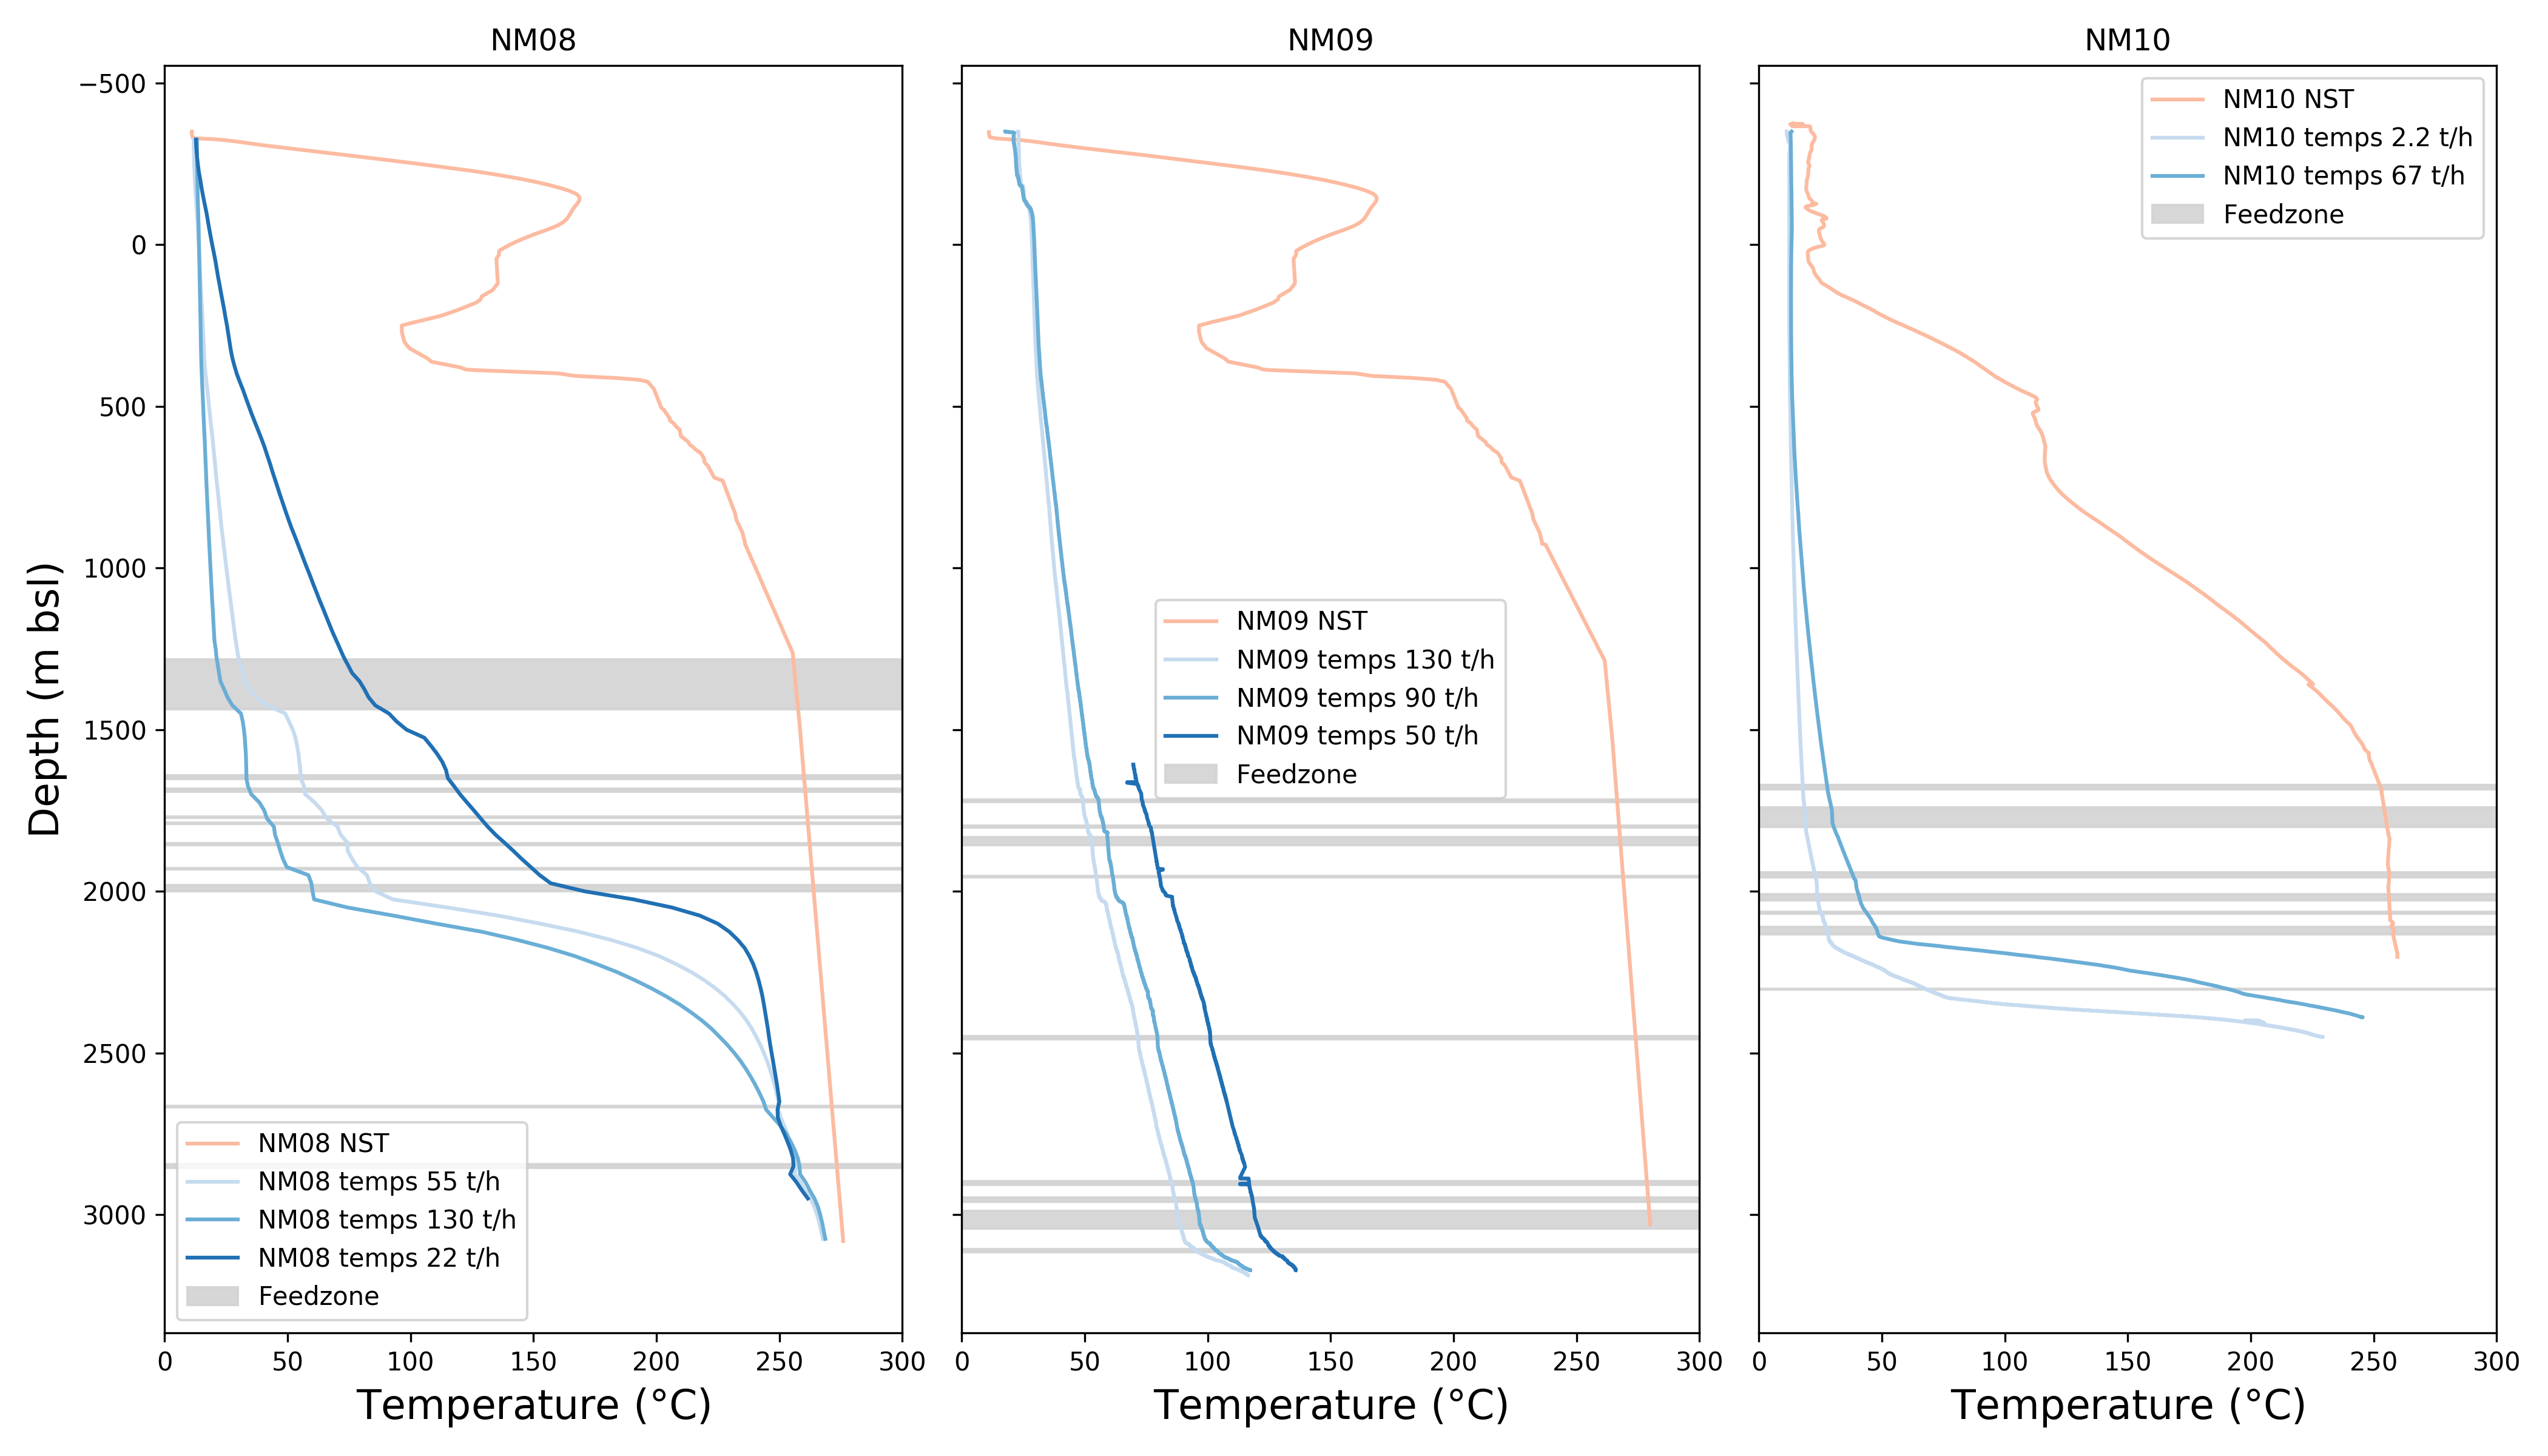
\includegraphics[width=\textwidth,height=\textheight,keepaspectratio]{Chapter_2_Data/figures/all_wells_Nga/all_wells_Nga_with_feedzones}
\caption[Example \acrfull{PTS} datasets]{{
Pressure-temperature spinner data recorded during completion tests at
each of the three wells drilled at Ngatamariki in 2012. The blue lines
indicate temperatures for fluid injected at various static \glspl{flow_rate}
and the orange lines represent combinations of measured and interpreted
natural state temperatures in the reservoir.
{\label{748181}}%
}}
\end{center}
\end{sidewaysfigure}

For a given \gls{flow_rate}, a strong variation in temperature over some depth interval typically implies that fluid is entering or leaving the well and that the corresponding depth may be a \gls{feedzone}. In the case of the injection tests shown in Figure \ref{748181}, strong `heating' signals with depth signify that a relatively large volume of cold injectate is moving from the well into the reservoir, leaving hotter, conductively-heated fluid in the wellbore at greater depths. This information constrains the points from which fluid flows, and therefore helps us to interpret where pressure signals originate and how they relate to the characteristics of seismicity.

\subsubsection{Image logs}
In the case of many geothermal reservoirs, including Ngatamariki and Rotokawa, \gls{permeability} is controlled by the reservoir fracture network. This is because the matrix rock is far less permeable than the typically extensive open fractures \citep{Grant_2011,Cant_2018}. A final important constraint on the locations of well \glspl{feedzone}, as well at the distribution and orientation of fractures over the entire reservoir, are resistivity- and sonic-based image logs. These logs are capable of showing detailed structures that intersect the wellbore including open (permeable) and sealed (impermeable) fractures and help corroborate data obtained from PTS measurements as to the location of \glspl{feedzone} (Figure \ref{746257}). These measurements of reservoir fracture orientations are also useful contraints on the structures available to slip, and therefore help to constrain fault plane ambiguity in focal mechanism results.\selectlanguage{english}

\begin{figure}[h!]
\begin{center}
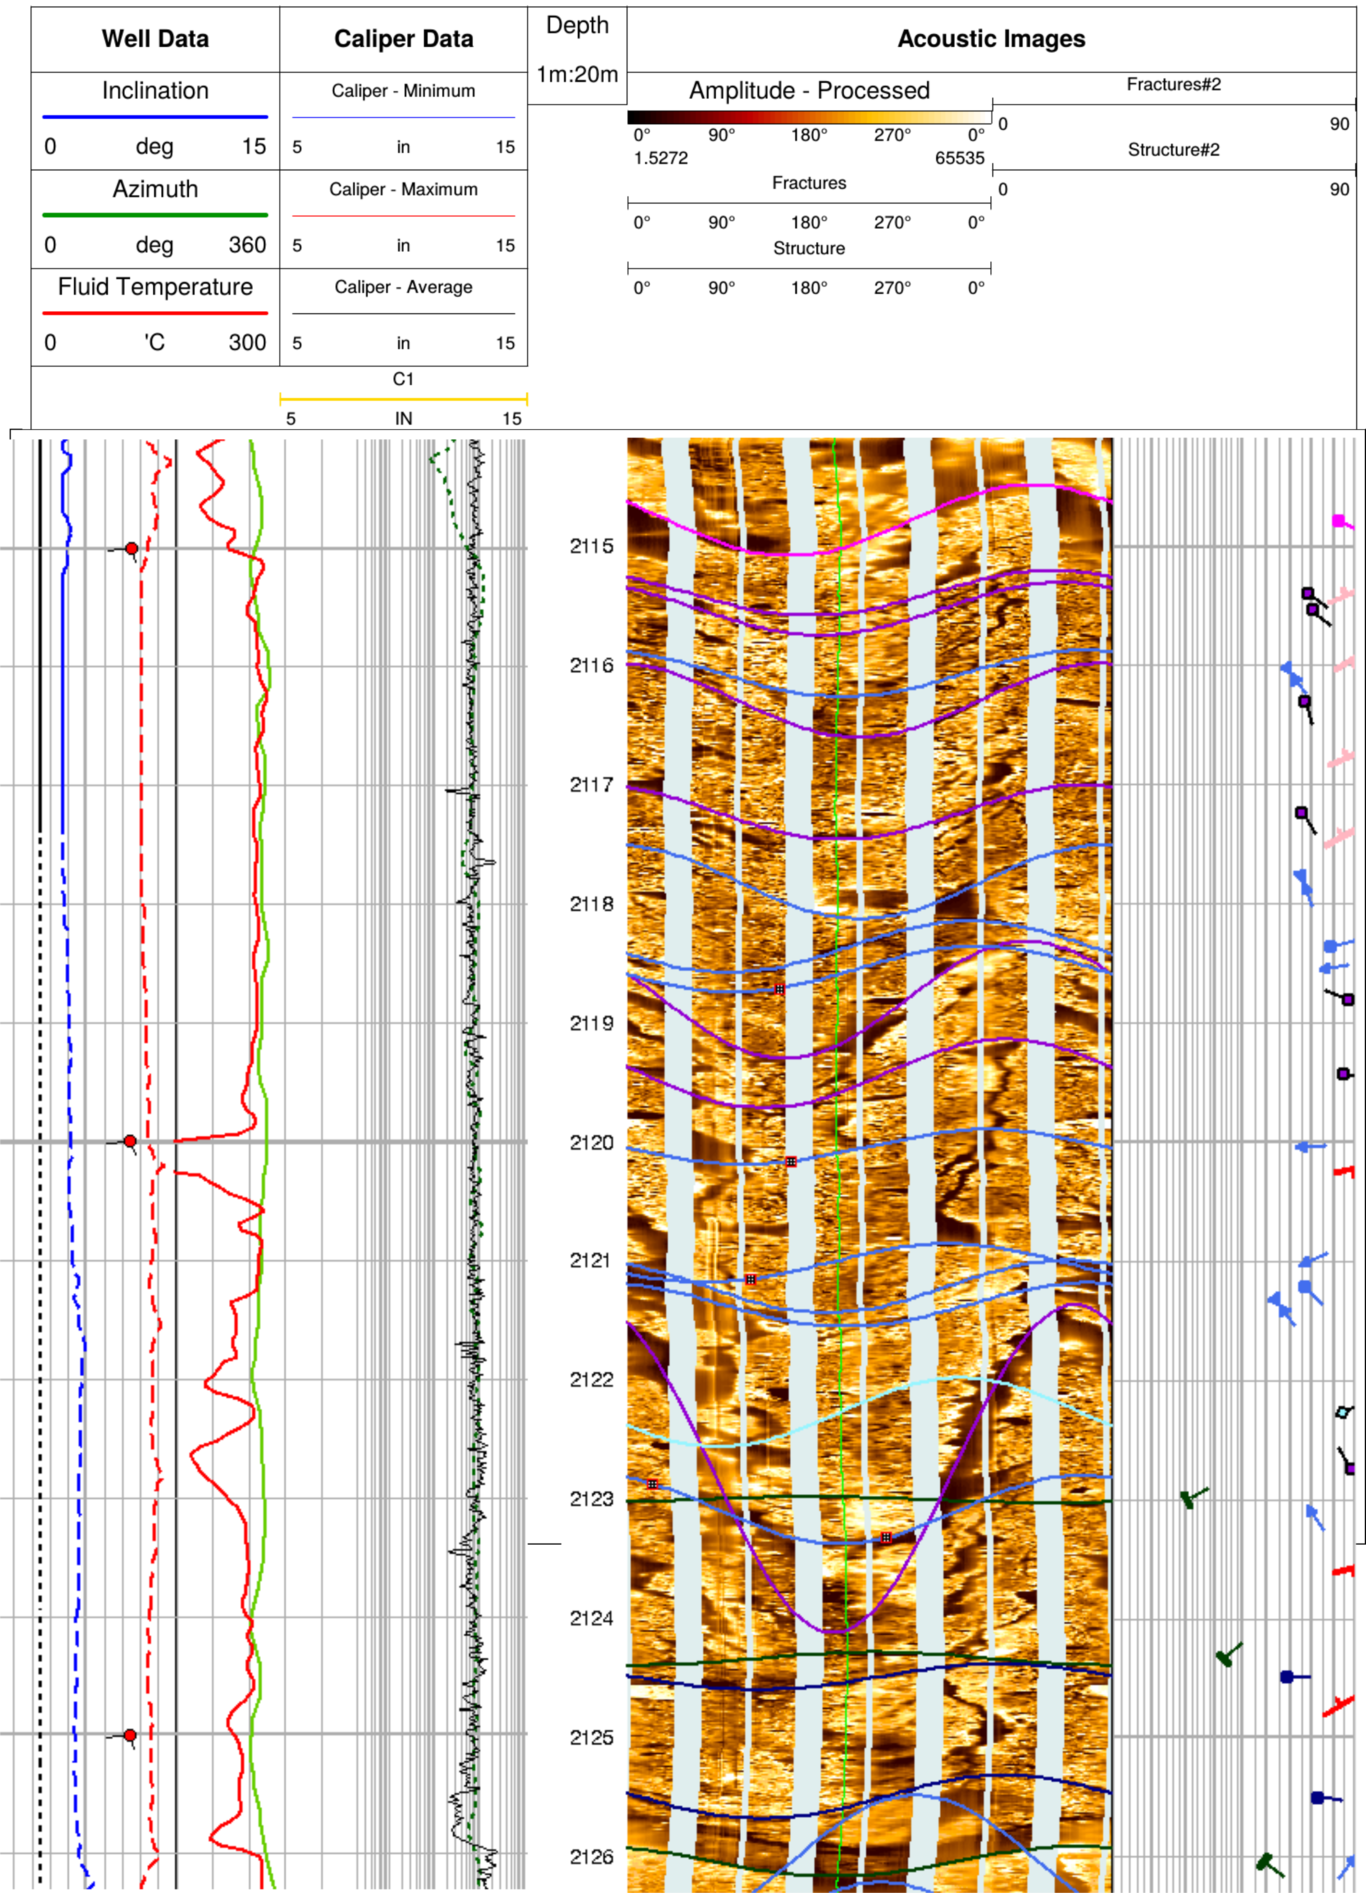
\includegraphics[width=0.70\columnwidth]{Chapter_2_Data/figures/FMI_example_mod/FMI_example_mod}
\caption[Example wellbore image data]{{
Example interval from the FMI image of Ngatamariki well NM10, showing
interpreted fractures as well as other borehole data collected during
the survey.
{\label{746257}}%
}}
\end{center}
\end{figure}

\section{Methods}
\subsection{Earthquake Detection}
In order to construct a catalog of induced seismicity, earthquakes must first be detected in a noisy stream of data that contains few signals of interest. Detection is perhaps the most important task in the seismological workflow, yet the variety of methods employed to this end are imperfect and constantly being revised. In this thesis, we make use of two methods of detection, energy-based and correlation-based, the second built upon the first.

\subsubsection{Energy-based}\label{STA/LTA}
The energy released in an earthquake is proportional to the amplitude of the signal recorded at a given seismograph station \citep{stein_2000}. It is therefore intuitive that earthquakes can be detected by looking for changes in the amplitude of a single stream of seismic data, with the important caveat that the earthquake must have released a sufficient amount of energy to produce a signal of larger amplitude than the noise in the recorded data. The most ubiquitous technique for detecting earthquakes based on amplitude change is known as the STA/LTA method, whereby amplitudes in two overlapping windows of different duration are compared \citep{withers1998comparison}. The ratio of the average amplitude of the short-term (STA) window to the long-term (LTA) window defines the detection statistic and a detection (sometimes referred to as a `trigger') is recorded when the statistic exceeds a user-defined value.

A subsequent step in earthquake detection is known as `association', which involves the grouping of triggers from multiple seismographs into distinct events. When only one or two triggers occur across a network, local noise sources may have triggered these stations, whereas the presence of many triggers across the network at a similar time likely signifies the occurrence of a larger phenomenon, perhaps an earthquake.

As mentioned above, the energy-based detection for this thesis was undertaken by GNS Science using the SeisComP3 software package. Triggering and station magnitude calculation was done using the module \textit{scautopick} and event association using the module \textit{scautoloc}, yielding the starting catalog for the correlation based detection undertaken next.

\subsubsection{Correlation-based (matched filter)}\label{MF}
Where a stream of seismic data contains high levels of noise (e.g. in areas of extensive industrial activity) or a large number of signals, such as within an aftershock sequence, energy-based detection cannot realistically detect many of the events present in the data. Waveform cross-correlation has been used to overcome these deficiencies in finding known signals in such settings, and has been applied widely to problems including radar, digital communications and astronomy \citep[e.g.][]{Turin_1960,Abbott_2016}. Correlating a known signal with a stream of data in search of a matching signal is often referred to as "matched-filter processing".

In seismology, matched filters have been adopted for use in finding a wide range of repeating and near-repeating signals that had eluded standard energy-based techniques, so long as the signal of interest was known. These applications include detection of local-to-regional scale crustal seismicity \cite{Schaff_2011,Dodge_2015,Chamberlain_2017}, low-frequency and non-volcanic tremor at plate boundaries \citep{Shelly_2007,Chamberlain_2014}, volcanic and volcano-tectonic signals \citep{Shelly_2016,Hotovec_Ellis_2018}, aftershock sequences \citep{Warren_Smith_2017} and explosions \citep{Gibbons_2006,Gibbons_2012}. In all instances, the known signal, be it an earthquake, radar pulse or nuclear explosion is referred to as the `template' and the discovered, previously unknown signals are termed `detections'. Throughout this thesis, we will also use the term `family' to mean all detections generated by a single template. Detections in the same family are shown for template 2012sora451121 in Figures \ref{434259} and \ref{233225}.\selectlanguage{english}

\begin{figure}[h!]
\begin{center}
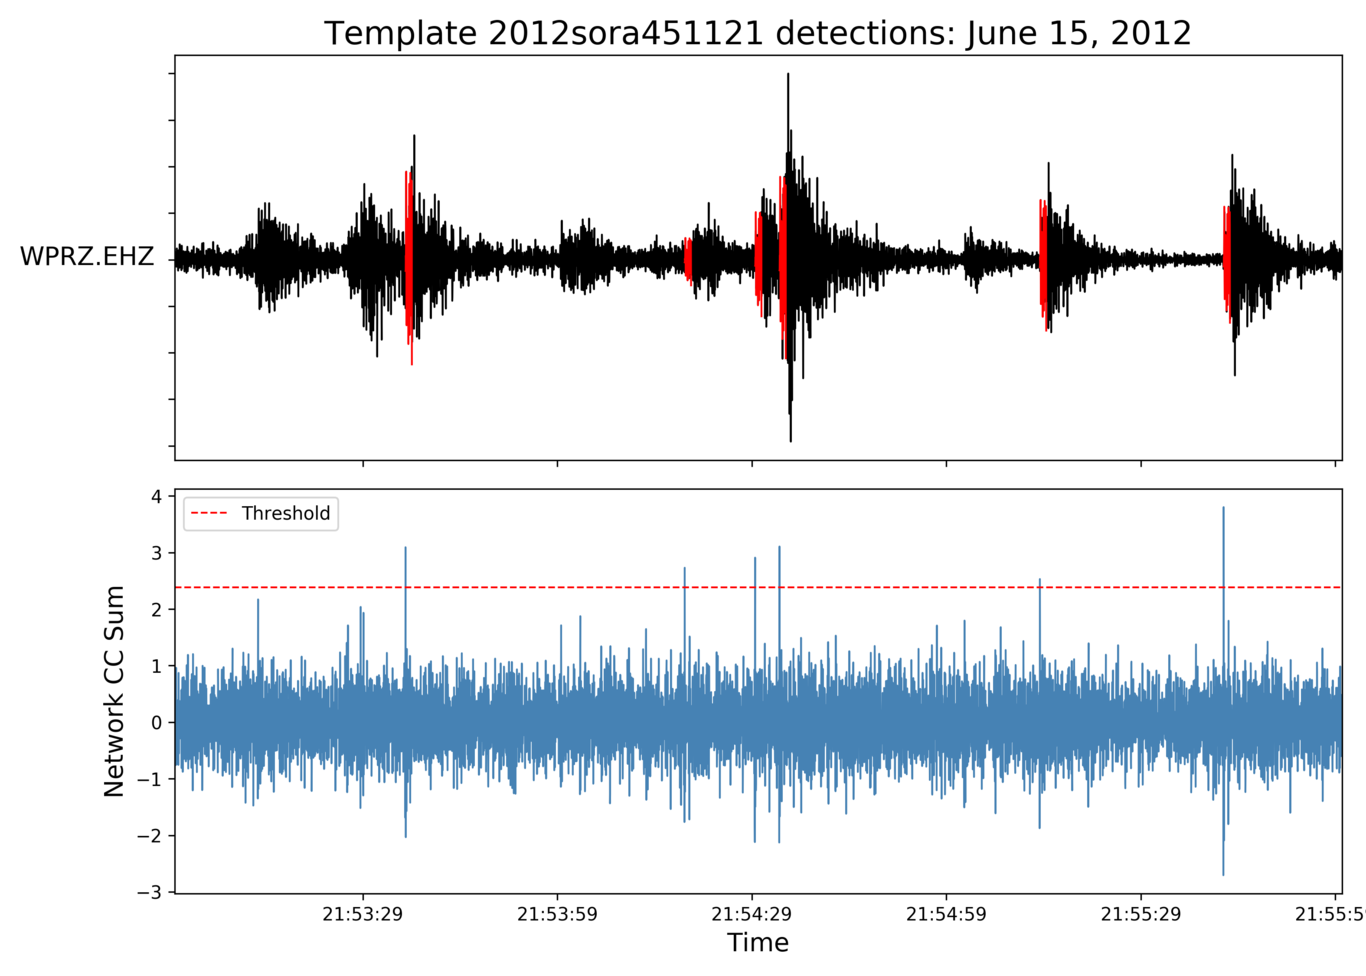
\includegraphics[width=0.70\columnwidth]{Chapter_2_Data/figures/2012sora451121_dets_cc_example/2012sora451121_dets_cc_example}
\caption[Example matched-filter detected waveforms]{{
Detections shown only at station WPRZ for template 2012sora451121 on 15
June 2012, during the stimluation of well NM08 (plot is three minutes
long). The top panel shows template waveforms (red) overlain on
continuous data (black). The bottom panel shows the cross-correlation
sum for the entire network in blue with the daily detection threshold
(MAD * 8) shown as a red dotted line.
{\label{434259}}%
}}
\end{center}
\end{figure}\selectlanguage{english}


\begin{figure}[h!]
\begin{center}
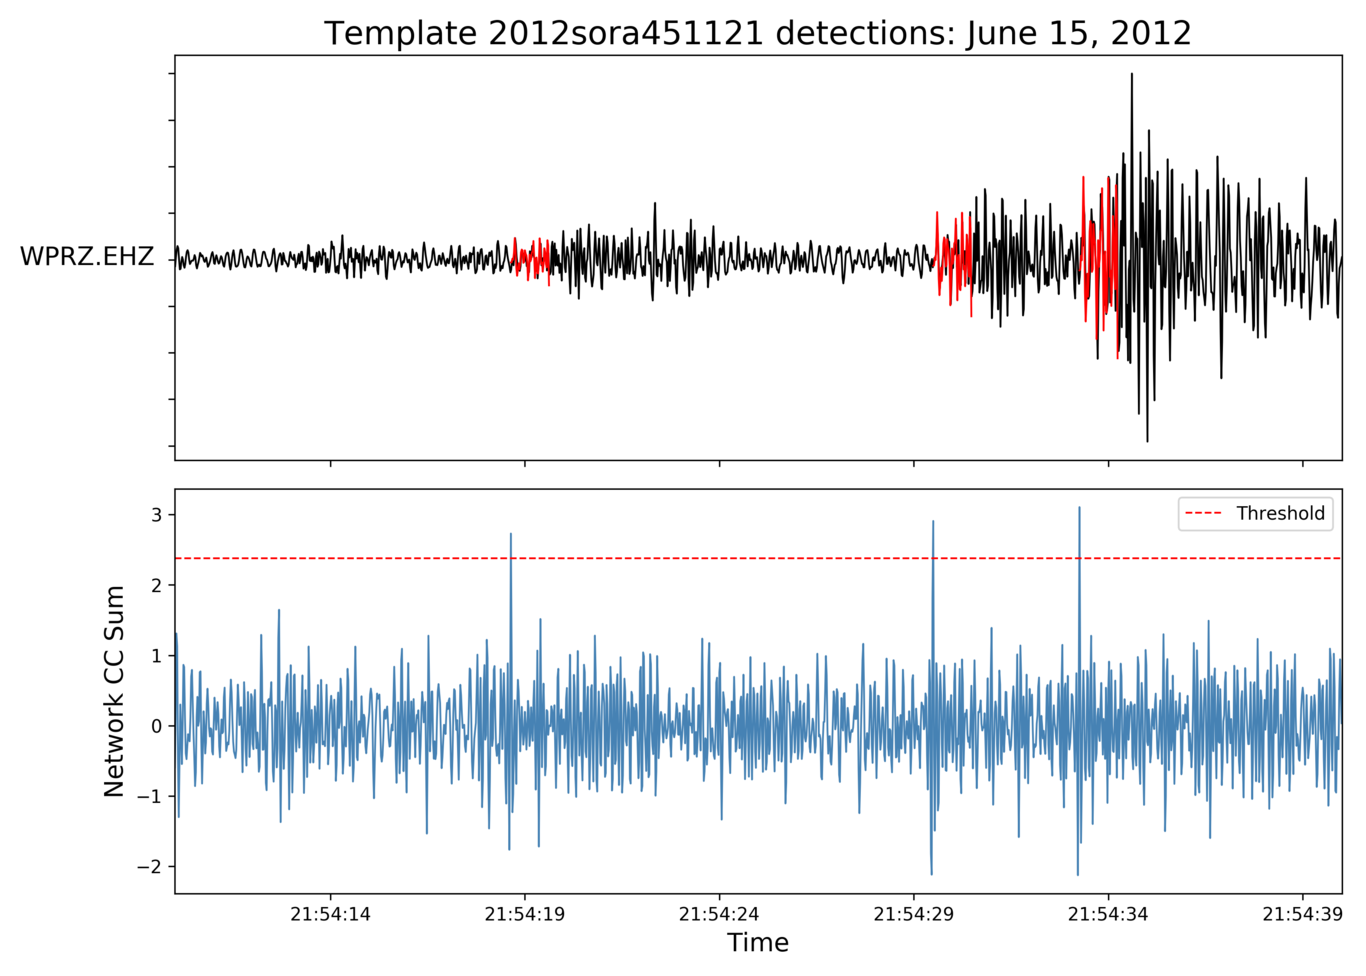
\includegraphics[width=0.70\columnwidth]{Chapter_2_Data/figures/2012sora451121_dets_cc_example_zoomed/2012sora451121_dets_cc_example_zoomed}
\caption[Close-up of matched-filter detections]{{
The same plot as above, zoomed into only 30 seconds including three
detections in order to show the waveforms in more detail.
{\label{233225}}%
}}
\end{center}
\end{figure}


In this thesis, we use the matched-filter method to detect repeating and near-repeating, shallow (\textless10km depth) crustal seismicity at the Rotokawa and Ngatamariki geothermal fields using the GNS-detected catalog described above as template events. The cross correlation between a template event at a single station and the continuous seismic data being searched is described by the following equation \citep{Chamberlain_2017}:

\begin{equation}
R(x) = \frac{\sum_{x'=0}^{x+w_{x}}(T'(x') \cdot I'(x + x'))}{\sqrt[]{\sum_{x'=0}^{x+w_{x}}(T'(x')^2 \cdot \sum_{x'=0}^{x+w_{x}}I'(x+x')^2}}
\end{equation}

Here $I'$ represents the continuous seismic data of interest and $T'$ represents the template earthquake. $x$ represents the sample in the continuous data between sample $0$ and sample $(N_{x} - w_{x})$, where $N_{x}$ is the length of the continuous data being searched and $w_{x}$ is the length of the template. $x'$ is the position within the window over which the correlation is being calculated.

This cross-correlation coefficient at each seismograph station is then summed to yield the network detection statistic (blue curves, Figures \ref{434259} and \ref{233225}). The threshold for declaring a detection is calculated as the median absolute deviation (MAD) of the detection statistic for the entire period being searched (one day, for instance), multiplied by a user-defined value. In this thesis, we use a detection threshold of MAD $*$ 8, as suggested by \citep{Shelly_2007} (red dotted line, Figures \ref{434259} and \ref{233225}).

The template waveforms used in our matched-filter routine are one second long, starting 0.1 seconds before the P-pick, when present. During the energy-based detection, P-picks were only made on vertical channels. Therefore, templates consist of only vertical channel waveforms (e.g. red waveforms in Figure \ref{249518}, \ref{434259} and \ref{233225}). Horizontal channels are not used due to the large uncertainties for the automatic S-picks in the GNS Science catalog. However, a length of one second ensures that both the P- and S-arrival are included in the template for each event due to the short travel times between events and stations at the geothermal fields (Figure \ref{955268}). A length of one second also omits much of the coda, which is incoherent, even between highly-similar sources. This is especially apparent at Ngatamariki and Rotokawa, due to the highly-fractured reservoir, large variations in the volcanic geology (e.g.\ welded ignimbrites and ashfall deposits) and surface-deposit heterogeneity. After applying an anti-aliasing filter, waveforms were resampled at 50 Hz and filtered from 3.0 to 20.0 Hz to accommodate the high corner frequencies of events with event-station distances of \textless15 km. Continuous seismic data were processed in an identical manner to the templates.\selectlanguage{english}

\begin{figure}[h!]
\begin{center}
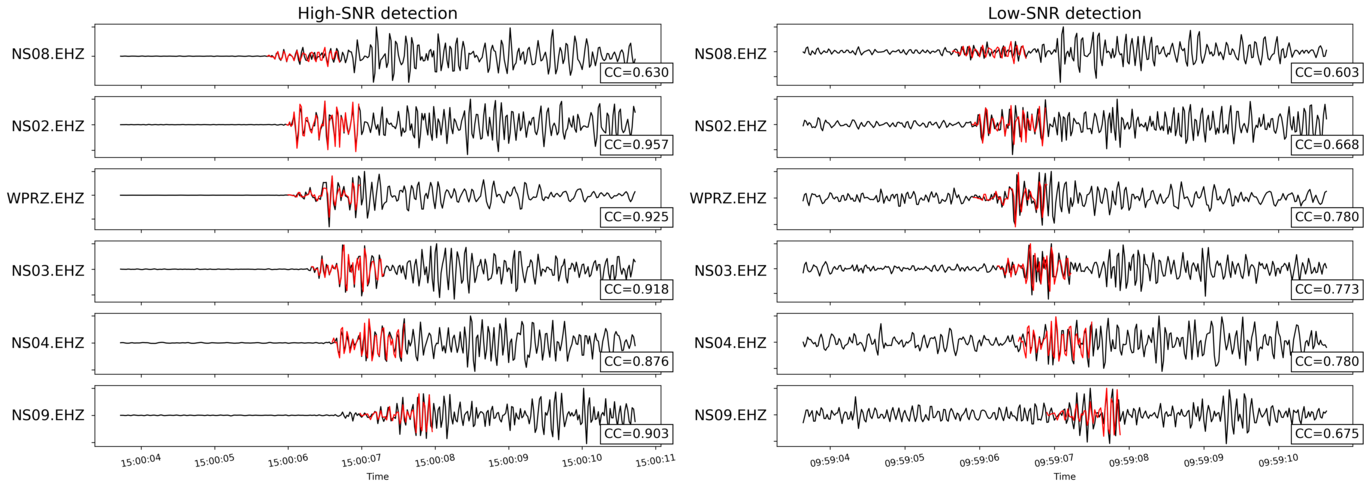
\includegraphics[width=0.98\columnwidth]{Chapter_2_Data/figures/det_example_publication/det_example_publication}
\caption[High and low signal-to-noise ratio detections]{{
Example detections of two events by template 2012sora469246
(signal-to-noise ratio of $\sim$50 and $\sim$3
respectively). The 1 s templates (in red) are overlain on 10 s of
continuous data around the time of detection (black). The ML 0.62
template event occurred on 22 June 2012 and detected mostly events that
occurred during the \gls{stimulation} of well NM08 between 6 June and early
July. The detection on the left represents a detection of a separate,
yet highly-similar, template event (template 2012sora469256) which
occurred approximately ten minutes after the template event shown here.
The detection on the right is a newly-detected event.
{\label{249518}}%
}}
\end{center}
\end{figure}

\subsection{Earthquake Location}
Once a signal has been detected, the most critical piece of information regarding the event is its location (or hypocenter), meaning its three-dimensional point of occurrence in space. The locations contained in an earthquake catalog reveal subsurface features such as faults or the geometry of a subducting slab, and spatio-temporal variations can reveal characteristics of dynamic triggering or fluid migration. The problem of determining an earthquake's location, in conjunction with its time of occurrence, can be forward modeled from estimated source parameters or inverse modeled from signal arrival times at a series of seismographs. The algorithms used to determine spatial location and origin time, collectively referred to solely as `location' here, can be broken into three groups.

\subsubsection{Linear methods}\label{linloc}
The most computationally efficient, and widely-used method for solving the non-linear location problem is to iteratively solve the forward problem posed in the following equation:

\begin{equation}
t_i = T + \frac{1}{v}\sqrt[]{(X - x_i)^2 + (Y - y_i)^2 + (Z - z_i)^2}
\end{equation}

where $t_i$ is the arrival time of the ray traveling between the earthquake and recording station $i$, treating the earth as a homogeneous half-space with wave speed $v$. $T$ is the source time of the earthquake, $(X, Y, Z)$ are the longitude, latitude and elevation of the earthquake and $(x_i, y_i, z_i)$ are the longitude, latitude and elevation of station $i$.

Using the above equation, the arrival time at each station can be calculated by `guessing' a starting location, $(X, Y, Z)$, and origin time, $T$. The difference between the known arrival time at a given station, ${t_i}^{obs}$, and the calculated arrival time, ${t_i}^calc$, (often referred to as the `misfit' or `time residual', $r_i$) defines the quality of the chosen starting location:

\begin{equation}
r_i = {t_i}^{calc} - {t_i}^{obs}
\end{equation}

Minimizing these residuals across a seismic network is the goal of all earthquake location approaches. The classical method used to solve the problem is an inverse approach, originally used by Geiger \citep{l1910,geiger1912probability}, whereby a system of equations taking the form:

\begin{equation}
r_i = \frac{\partial{t_i}}{\partial{X}}\Delta{X} + \frac{\partial{t_i}}{\partial{Y}}\Delta{Y} + \frac{\partial{t_i}}{\partial{Z}}\Delta{Z} + \Delta{t_0}\label{eq:3}
\end{equation}

is solved iteratively until some condition, typically a threshold misfit value or location adjustment, is met. $(\Delta{X}, \Delta{Y}, \Delta{Z}, \Delta{t_0})$ are the adjustments in the starting location parameters between iterations and the partial derivatives are expressed as follows:

\begin{equation}
\frac{\partial{t_i}}{\partial{X}} = \frac{X - x_i}{vS}
\end{equation}
\begin{equation}
\frac{\partial{t_i}}{\partial{Y}} = \frac{Y - y_i}{vS}
\end{equation}
\begin{equation}
\frac{\partial{t_i}}{\partial{Z}} = \frac{Z - z_i}{vS}
\end{equation}

where $S$ represents the length of the source-receiver path.

Geiger's original method solved the problem via a least-squares approach, although many other methods have been proposed and used since, including adding damping parameters and solving via singular-value-decomposition \citep{thurber1985nonlinear}.

For real-world scenarios, the above equations oversimplify the problem of earthquake location because they assume the velocity of the subsurface is homogeneous. For most locations where earthquakes occur, the substrate is heterogeneous, consisting of horizontal layers (as the simplest case) and growing in complexity to include strong lateral heterogeneities as well (faults, for example). This velocity heterogeneity is approximated by a velocity model, which expresses velocity changes with depth (1-dimensional) and sometimes with geographic location as well (2- and 3-D cases).

For this thesis, the original linearized locations are calculated in SeisComP3 via the algorithm of \citet{Lee_1972}, which uses a step-wise regression approach, and a velocity model calculated for the entire Taupo Volcanic Zone \citep{Sherburn_2003}. For further relocations, we use a simple, 1-dimensional velocity model provided by \citet{sewell2017} specifically for our seismic network (Table \ref{vmod}).\selectlanguage{english}

\begin{table}
\centering
\begin{tabular}{cc}
    {Layer top (km)} & {$V_{P}$ (km/s)} \\ \midrule
    -0.6  & 1.9 \\
    0.2  & 2.6  \\
    1.0  & 3.5  \\
    1.5  & 3.6  \\
    2.0  & 3.9   \\
    3.0  & 4.9  \\
    5.0  & 5.4  \\
    10.0  & 5.81  \\
    20.0  & 6.9  \\
    50.0 & 7.43   \\
\end{tabular}
\caption[1-D velocity model used in this thesis]{{
Local 1-D velocity model for Ngatamariki and Rotokawa from VELEST inversions}}
\label{vmod}
\end{table}

\subsubsection{Non-linear methods}
In cases where the velocity model is poorly known, velocity structure is highly-variable, earthquake locations are shallow or are outside of the seismic network, the linearization approaches described above may be insufficient to address a more highly-nonlinear location problem \citep{thurber1985nonlinear}. In this case, a number of additional approaches may be used. \citet{thurber1985nonlinear}, for example, suggested including the second order terms corresponding to the first-order Taylor series expansion described in Equation \ref{eq:3}. These second-order terms can be especially important for shallow earthquakes located within a local seismic network and for short source-receiver paths. Foregoing linearization completely, \citet{tarantola1982inverse} suggested a probabilistic approach whereby the posterior \acrfull{pdf}, $Q$, of the four unknown parameters (i.e. three spatial dimensions plus time) is described by \citep{Lomax_2014}:

\begin{equation}
    Q(\mathbf{m}) = k\:p(\mathbf{m}) \int_{\mathbf{D}}^{} \frac{p(\mathbf{d})F(\mathbf{d},\mathbf{m})}{\mu(\mathbf{d},\mathbf{m})} d\mathbf{d}
\end{equation}

where $k$ is a normalization constant, $\mathbf{m}$ is the vector of unknown hypocentral parameters, $\mathbf{d}$ is the vector of observed arrival-time data, $p(\mathbf{d})$ is the \acrshort{pdf} describing the arrival-time uncertainties and $p(\mathbf{m})$ represents prior information about the hypocenter (e.g. from damage reports or known fault parameters). $F(\mathbf{d},\mathbf{m})$ is the ability of the forward problem to describe the arrival times and $\mu(\mathbf{d},\mathbf{m})$ is the homogeneous distribution over the arrival time data and hypocentral parameters \citep{Lomax_2014}. The integral over the dataspace, $\mathbf{D}$ is typically referred to as the `likelihood function', $L(\mathbf{x})$, and describes how well the given hypocenter represents the data.

For this thesis we have chosen to use the location program \textit{NonLinLoc} \citep{Lomax_2000}, which makes use of the solution presented above and uses one of a number of grid search algorithms to interrogate one of two possible likelihood functions, $L(\mathbf{x})$, one based on an L2-norm misfit function \citep{tarantola1982inverse} and the other given by Equation \ref{likelihood}. We have chosen to use this `equal-differential time' likelihood function as it is more robust to outliers in the arrival time data \citet{Lomax_2014}:

\begin{equation}\label{likelihood}
    L(\mathbf{x}) = \Bigg[\sum_{a,b}^{}\frac{1}{\sigma_{a}^{2} + \sigma_{b}^{2}} \cdot \exp \Bigg(-\frac{\{[T_{a}^{o} - T_{b}^{o}] - [TT_{a}^{c}(\mathbf{x}) - TT_{b}^{c}(\mathbf{x})]\}^{2}}{\sigma_{a}^{2} + \sigma_{b}^{2}}\Bigg)\Bigg]^{N}
\end{equation}

where $\mathbf{x}$ are the three spatial parameters of $\mathbf{m}$. The sum is taken over all possible ($N$) observation pairs, $a$ and $b$, where $T_{a}^{o}$ and $T_{b}^{o}$ are the observed arrival times and $TT_{a}^{c}$ and $TT_{b}^{c}$ are the calculated travel times (arrival time minus the time of the event) for each observation, respectively. $\sigma_{a}$ and $\sigma_{b}$ represent the uncertainties of the observed arrivals times and calculated travel times \citep{Lomax_2014}. The likelihood function maximizes where the difference in arrival times, $[T_{a}^{o} - T_{b}^{o}]$, and difference in calculated travel times, $[TT_{a}^{c}(\mathbf{x}) - TT_{b}^{c}(\mathbf{x})]$, are equal, corresponding to the point in space, $\mathbf{x}$, that best represents observations $a$ and $b$. After summing over all possible pairs, the resulting \acrshort{pdf} has maxima at the spatial locations that satisfy the largest number of observation pairs, but does not attempt to fit all observations at once, making it more robust in the presence of arrival-time outliers. This formulation also eliminates the calculation of the event origin time, reducing the the location problem from four to three dimensions \citep{Lomax_2014}. 

\textit{NonLinLoc} first computes the travel times to all stations for each node in a user-defined grid. As the user may then attempt to solve the location problem using a number of gridding approaches, we selected the OctTree gridding method for all events at Rotokawa and Ngatamariki. The OctTree approach first calculates the probability that the source lies within any node in a coarse grid encompassing the entire, user-defined search area. This probability is proportional to the volume of the node and inversely proportional to the travel-time misfit calculated at its center \citep{Lomax_2000}. The highest-probability node is then divided into eight equal-volume sub-nodes and the process is repeated, dividing the most likely of the sub-nodes into eight and continuing this process until a threshold is reached and the maximum-likelihood hypocenter found. Typically, the threshold for halting the program is a minimum node volume. \textit{NonLinLoc} then samples the resulting OctTree structure of searched nodes in order to provide a representation of the location probability density function, which can then be used to characterize the uncertainty in the hypocenter solution \citep{Lomax_2000}.

\subsubsection{Relative location methods}
Perhaps the most significant uncertainty inherent in the location problem is that associated with the subsurface velocity structure. In an attempt to minimize the effect this uncertainty has on calculated locations, relative location methods have been developed, the most widely used of which is the double-difference method. Instead of minimizing the misfit between observed and calculated arrival times for a single event, double-difference techniques seek to minimize the misfit between the observed and calculated arrival time \textit{differences} between two paired events (hence, double-difference). The most popular of the double-difference location programs is \textit{HypoDD} \citep{Waldhauser_2000}, which attempts to solve the (oftentimes large) system of equations defining a web of interconnected pairs of events by minimizing the L2 norm of the double-differences.

A recent, alternative approach to the double-difference problem is the \textit{GrowClust} algorithm developed by \citet{Trugman_2017}, which we use for the final relocations of the catalogs presented in this thesis. The \textit{GrowClust} algorithm makes use of the same data as \textit{HypoDD}, namely travel-time differences between pairs of events, as well as absolute travel time data and starting locations. However, instead of attempting to solve the entire system of equations defined by every event pair, \textit{GrowClust} creates a list of event pairs in order of descending similarity (defined as the sum of the cross-correlation coefficients between their common waveforms). It then relocates each event pair, or cluster pair where an event pair joins two preexisting clusters, relative to each other by minimizing the L1 norm (which is more robust to outliers than the L2 approach). Finally, \textit{GrowClust} also includes location error estimates via an iterative bootstrapping procedure that randomly resamples the input data and relocates the catalog. The location uncertainty is reported as the median absolute deviation of each event's location for each of the $n$ user-defined bootstrap iterations.

Application of these relative location techniques often proves imperative to obtaining precise locations, thus illuminating small-scale structures and migration of seismicity with time. Without these techniques, it can be difficult to interpret location results with any degree of confidence, especially at scales of \textless{10}km, as at Rotokawa and Ngatamariki.

\subsection{Magnitude calculation}
The calculation of earthquake magnitude is typically done in conjunction with its detection and location and is the final, key parameter required for analysis of any earthquake catalog. There are a number of ways in which earthquake magnitude is calculated, usually based on the measured maximum amplitude of a signal recorded at a number of seismograph stations, but it can also be based on other measurements such as signal duration or full moment tensor inversion \citep{Kanamori_1983}. In this thesis, magnitudes for the GNS-located template events are reported at local magnitudes (M$_L$), and discussed in detail in Section \ref{GNS_cat}.

To compute the magnitude of the events detected by the matched filter,
we use the method described by \citet{Shelly_2016}, which uses pair-wise relative amplitudes between a template event and each of its detections to compute relative moments (Figure \ref{svd_mags}). This approach computes the relative amplitude, $\alpha$, as

\begin{equation}
\alpha = v[2] / v[1]
\end{equation}

where $v[2]$ and $v[1]$ are the second and first elements, respectively, of the first row of the 2$\times$2 matrix $V'$ in

\begin{equation}
M = U\Sigma V'
\end{equation}

representing the singular value decomposition of a data matrix, $M$, with columns comprising both the template and the detected waveform on a single channel (Figure \ref{svd_mags}). The rows of $V'$ are the right singular vectors, which map the weight of the left singular vectors, $U$, to the original data vectors and $\Sigma$ is a set of nonnegative singular values. Because the template and detected waveforms in the data matrix are inherently similar, the first left singular vector, $U_0$, should describe only a difference in amplitude between template and detection. The relative amplitude between the two events can therefore be estimated as the ratio of the second and first elements, $v[2]$ and $v[1]$, of the first row of $V'$.

\begin{figure}[h!]
\begin{center}
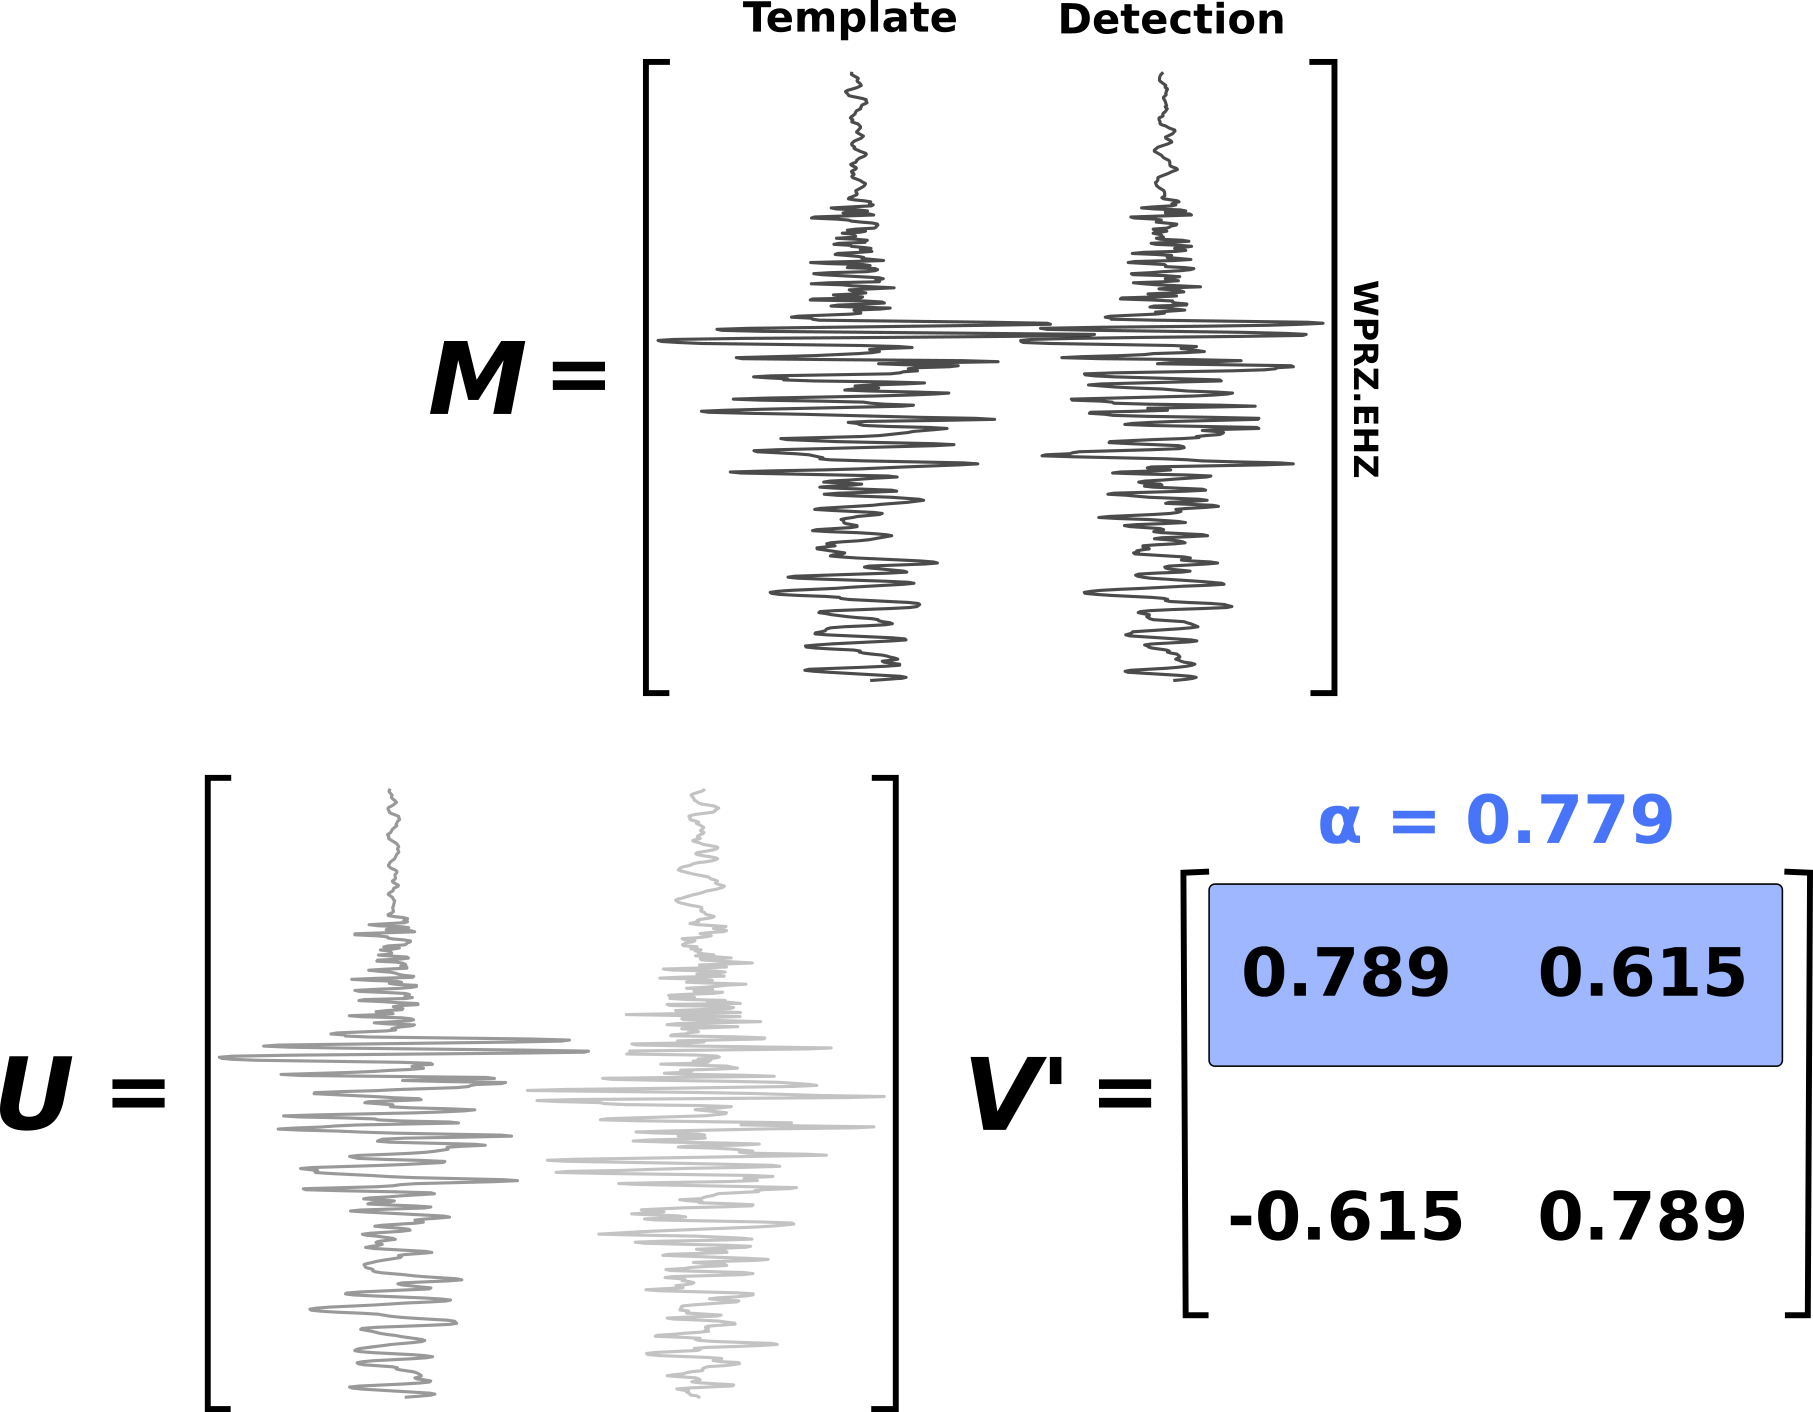
\includegraphics[width=0.98\columnwidth]{Chapter_2_Data/figures/mag_calc_example/mag_calc_example_2012sora451121}
\caption[Relative amplitude calculation]{{
Illustration of the relative amplitude calculation between template and detected events with real waveforms and values. The matrix, \textbf{M}, is the data matrix, in our case with the waveforms as columns. The singular value decomposition comprises the left singular vectors (as columns of $U$), the corresponding eigenvalues, ($\Sigma$; not shown) and the right singular vectors (as rows of $V'$). The columns of $U$ effectively describe the signal that both the template and detection have in common, with decreasing importance from left to right. The rows of $V'$ represent the contribution of the columns of $U$ to each column of $M$. As the template and detected waveforms are inherently similar, the first column of $U$ describes the bulk of their signals and therefore the first row of $V'$ describes their relative amplitudes.
{\label{svd_mags}}%
}}
\end{center}
\end{figure}

We calculate relative amplitudes only when the cross-correlation coefficient between the template and detection exceeds 0.6 at any given station. Again, we note that template events only contain waveforms for the vertical channels. For those events recorded by a minimum of four stations exceeding the correlation threshold, we calculate the relative moment as the median of the relative amplitudes, following \citet{Shelly_2016}. We note that, because the relative amplitudes are calculated from two waveforms recorded at the same station, there is no need to remove the instrument response.

This approach has proven to be more robust in the presence of relatively dissimilar waveforms than the method of \citet{Rubinstein_2010}, for example, which assumes high correlation coefficients between all pairs of events in a family (e.g.\ $\geq$0.85) instead of simply between a template and each single detection, as assumed here. At Rotokawa and Ngatamariki, scattering and attenuation effects produce waveforms exhibiting lower degrees of similarity than typical repeating or near-repeating seismicity (e.g.\ along the San Andreas \citep{Rubinstein_2010}).

We use the GNS Science $M_{L}$ (as described in Section \ref{GNS_cat}) to calibrate the relative moment calculations from the method above and produce $M_{L}$ estimates for the matched-filter detections. This is done by first converting the template $M_{L}$ to $M_{w}$ using the scaling relationship \citep{Ristau_2009}:

\begin{equation}
M_{L} = 0.88M_{w} + 0.73
\end{equation}

determined for locally detected, shallow New Zealand earthquakes and then converting to seismic moment using the equation \citep{Hanks_1979}:

\begin{equation}
M_w = \frac{2}{3}\log_{10}M_{0} - 9
\end{equation}

Knowing the relative moment of the template event from the procedure outlined above, we then determine the relationship between the relative moments and actual moment which allows us to convert relative moments to $M_w$ and then back to $M_L$ using the relationship of \citet{Ristau_2009}.

\subsection{Focal mechanisms}
The final step taken in developing the earthquake catalog presented here is the determination of earthquake focal mechanism solutions. The shear displacement on a fault is often represented as a point acted on by two perpendicular force couples (the so-called double-couple source), by ignoring any potential volumetric changes associated with the event \citep{stein_2000}. The energy radiated by such a double-couple source can be divided into four quadrants: two dilational and two compressional. At a given seismic station, the ground displacement from an arriving P-wave depends on which of the quadrants the path between the source and receiver emanated from. If that path emanated from a compressional quadrant the ground will move upwards, and if the path emanated from a dilational quadrant, the ground will move downwards. Therefore, by observing the pattern of first motion polarities (up or down) recorded across a seismic network, constraints can be placed on the orientation of the fault that slipped and the direction of slip associated with the corresponding earthquake \citep{stein_2000}.

A number of approaches have been developed to invert polarity recordings for the fault plane orientation of an earthquake, typically by forward modeling a large number of possible sources to find the mechanism which best fits the polarity observations \citep[e.g.][]{Reasenberg_1985,Hardebeck_2002}. The focal mechanism solutions presented in this thesis were calculated using the Bayesian approached developed by \citet{Walsh_2009}, which allows for the incorporation of known uncertainties in the input parameters (e.g. earthquake location and first arrival picks) and outputs a \acrshort{pdf} of the focal mechanism solution.
% 	\cleardoublepage
% 	\chapter[Seismic response to injection well stimulation in a high-temperature,
high-permeability reservoir]{Seismic response to injection well \\ stimulation in a high-temperature,
\\high-permeability reservoir}

\section*{Abstract}
Fluid injection into the earth's crust can induce seismic events that
cause damage to local infrastructure but also offer valuable insight
into seismogenesis. The factors that influence the magnitude, location
and number of induced events remain poorly understood but include
injection flow rate and pressure as well as reservoir temperature and
permeability. The relationship between injection parameters and
injection-induced seismicity in high-temperature, high-permeability
reservoirs has not been extensively studied. Here we focus on the
Ngatamariki geothermal field in the central Taup\={o} Volcanic Zone, New
Zealand where three stimulation\slash{injection} tests have occurred since
2012. We present a catalog of seismicity from 2012-2015 created using a
matched-filter detection technique. We analyze the stress state in the
reservoir during the injection phases from first-motion-derived focal
mechanisms, yielding an average direction of maximum horizontal
compressive stress (S\textsubscript{HMAX}) consistent with the regional
NE-SW trend. However, there is significant variation in the direction of
maximum compressive stress (\(\sigma_{1}\)), which may reflect
geological differences between wells. We use the ratio of injection flow
rate to overpressure, referred to as injectivity index, as a proxy for
near-well permeability, and compare changes in injectivity index to
spatiotemporal characteristics of seismicity accompanying each test.
Observed increases in injectivity index are generally poorly correlated
with seismicity, suggesting that the locations of microearthquakes are
not coincident with the zone of stimulation (i.e. increased
permeability). Our findings augment a growing body of work suggesting
that aseismic opening or slip, rather than seismic shear, is the active
process driving well stimulation in many environments.

\section{Introduction} \label{Intro}
In recent years, the number of recorded cases of injection-induced seismicity has grown dramatically with the proliferation of industrial activities such as wastewater disposal and enhanced geothermal systems (EGS) \citep{Ellsworth_2013}. In many cases, most notably in the central US and Europe, these activities have induced events that caused damage to local infrastructure and even a number of injuries \citep[e.g.][]{Keranen_2013,Hsieh_1981,Deichmann_2009}. However, these injections also offer valuable insight into seismogenesis, which may help to better manage future injection-induced seismic hazard. While most case studies have addressed low-temperature, high-permeability reservoirs such as the Arbuckle group in Oklahoma \citep[e.g.][]{Langenbruch_2016} or medium-temperature, low-permeability reservoirs targeted at EGS sites \citep[e.g.][]{Deichmann_2009,Evans_2005}, here we present a case of induced seismicity related to injection operations in the high-temperature, high-permeability Ngatamariki geothermal reservoir. Though seismicity associated with such reservoirs has been well documented for decades (for example, at The Geysers field in California), most studies have needed to consider simultaneous injection from multiple wells with long histories of injection, thereby complicating the relationship between induced seismicity and injection parameters such as flow rate and wellhead pressure (WHP) \citep[e.g.][]{Allis_1982,Mart_nez_Garz_n_2014, Kwiatek_2015,Mart_nez_Garz_n_2017}. Here we present a much simpler case study involving multiple injections isolated from one another in both space and time.

The aim of underground fluid injection is typically to dispose of unwanted fluids or to increase permeability at depth \citep{Ellsworth_2013,Grant_2011}. In the geothermal industry, an increase in permeability allows for more fluid to be injected or produced, thus reducing the number of wells required per unit of electrical generation. Fluid injection drives a number of processes that contribute to the occurrence of seismicity, including pore-fluid pressure increases, reservoir volume changes (due to injection or extraction of fluid), reservoir temperature decreases and chemical changes to fracture surfaces \citep{Majer_2007}. The conditions under which these processes induce seismicity and the relationship between seismic or aseismic slip and reservoir properties such as fracture permeability remain unclear \citep[][and references therein]{Amann_2018,Das_2011}. Unraveling these potential relationships is important in order to better plan future geothermal resource development, and has implications for deep injection operations and the understanding of seismogenesis in general.

The Ngatamariki geothermal field in the central Taup\={o} Volcanic Zone of New Zealand is a convenient place to study induced seismicity. Prior to our study period, which extends from June 2012 until the end of 2015, the development of the Ngatamariki resource had been limited to resource exploration in the 1980s followed by the drilling of three deep exploration wells (NM05, NM06, NM07 to $\sim$3km depth) in the 2000s \citep{Chambefort_2016}. The start of injection operations in 2012 represented the first large-scale fluid injection into the undisturbed, high-temperature ($\sim$280\textdegree) Ngatamariki reservoir \citep{Bignall_2009}. Fluid injection at three of the four major injection wells (NM08, NM09 and NM10) was undertaken in advance of the Ngatamariki power plant's commissioning in 2013. Pressure and flow rate during each of these operations was well-recorded (5 min resolution). As each operation occurred in isolation, the task of relating temporal and spatial patterns of microseismicity to injection parameters for a specific well was straightforward. Seismic data were recorded throughout these injections, enabling us to detect and precisely locate a large number of induced microearthquakes.

In the Ngatamariki case, the objectives of individual injection operations differed. Generally, these injections can be divided into three categories: cold-water stimulation, injection testing, and unintended fluid losses during drilling. Cold-water stimulation is a process intended to increase the permeability in a given well, and which is thought to be driven by the thermal contraction of reservoir rocks \citep{grant2013thermal}. Injection testing, while often conducted in conjunction with stimulation, is aimed at determining the injectivity index of a well, which is normally defined as the ratio of flow rate to well head pressure. This parameter is then used as an indicator of a well's bulk permeability and to predict injection well performance once a power plant begins operation. Fluid losses during drilling are generally unintended and result from the escape of drilling fluid into the formation as the well is drilled. Each of these scenarios occurred at Ngatamariki prior to the startup of the 82 MWe (``megawatts electrical") power plant in April of 2013. As we show below, the rate, location and magnitude of microseismicity associated with each individual injection operation were distinct, demonstrating differences in local geology, near-well permeability, fluid injection rate, history of injection and the temperature and chemistry of the injected fluid in each well.

In this paper, we construct a catalog of induced seismicity at Ngatamariki and compare the characteristics of seismicity to flow rate, pressure and injectivity index measured during three phases of injection prior to the startup phase of the Ngatamariki power plant. The temporal isolation of each phase of injection allows us to relate near-well seismicity to high-resolution injection parameters without contamination from multiple, concurrent injections. Given that the Ngatamariki reservoir occupies the upper end of both the temperature and permeability continuum, the injection-seismicity relationship here serves as a useful comparison to results from lower-temperature and lower-permeability settings elsewhere. Therefore, our results help to distinguish the importance of reservoir permeability and temperature in forecasting the extent and magnitude of induced seismicity during future injection operations.

\subsection{Geological and geophysical setting} \label{Setting}
The Ngatamariki geothermal field is located in the central Taup\={o} Volcanic Zone (TVZ) on the North Island of New Zealand, approximately 17 km north of the town of Taup\={o} (Figure \ref{795275}). Ngatamariki is a high-temperature, liquid-dominated and naturally-fractured system (280\textdegree{}C at depths exceeding 1000 m) that measures roughly 5.5 km from north to south and 3 km from east to west \citep{Bignall_2009,Chambefort_2014}. The reservoir is hosted in a succession of volcaniclastics known as the Tahorakuri formation, which exhibits significant lateral heterogeneity \citep{Chambefort_2014}. In the south, the deeper portions of the reservoir (\textless2000 meters below sea level) are hosted in the Rotokawa Andesite. In this part of the field, the Rotokawa Andesite overlies greywacke basement, which has been encountered in only one well (NM06) at 3012 m below sea level \citep{Chambefort_2014}. The geologic structure of the southern end of the field, between the central production wells and injection wells NM06 and NM10, is dominated by the active, NE--SW-striking Aratiatia Fault Zone (Figure \ref{795275}). Reservoir tracer tests have demonstrated the presence of high permeability between injection well NM10 and production well NM05 along an Aratiatia Fault Zone-related structure \citep{buscarlet_2015}. In the north, in the vicinity of injection wells NM08 and NM09, the reservoir geology is dominated by a shallow intrusive body (\textless 2000 m bsl), the presence of which was confirmed by drill cuttings and core in NM08, NM09 and NM04 \citep{Bignall_2009,Chambefort_2014}. The intrusive body lacks appreciable permeability itself, but it is enveloped by a highly-fractured damage zone that was encountered in wells NM08 and NM09 \citep{Clearwater_2015}. Given the low permeability of the reservoir matrix, typical of the TVZ \citep{Sibson_2003}, fluid flow is controlled by fractures and faults. Regionally, faults follow a NE--SW structural trend and borehole image logs at Ngatamariki indicate mostly NE--SW oriented fractures within the reservoir, with some variability with depth in certain wells \citep{Bignall_2009,Massiot_2015,massiot_2012}.\selectlanguage{english}

\begin{figure}[h!]
\begin{center}
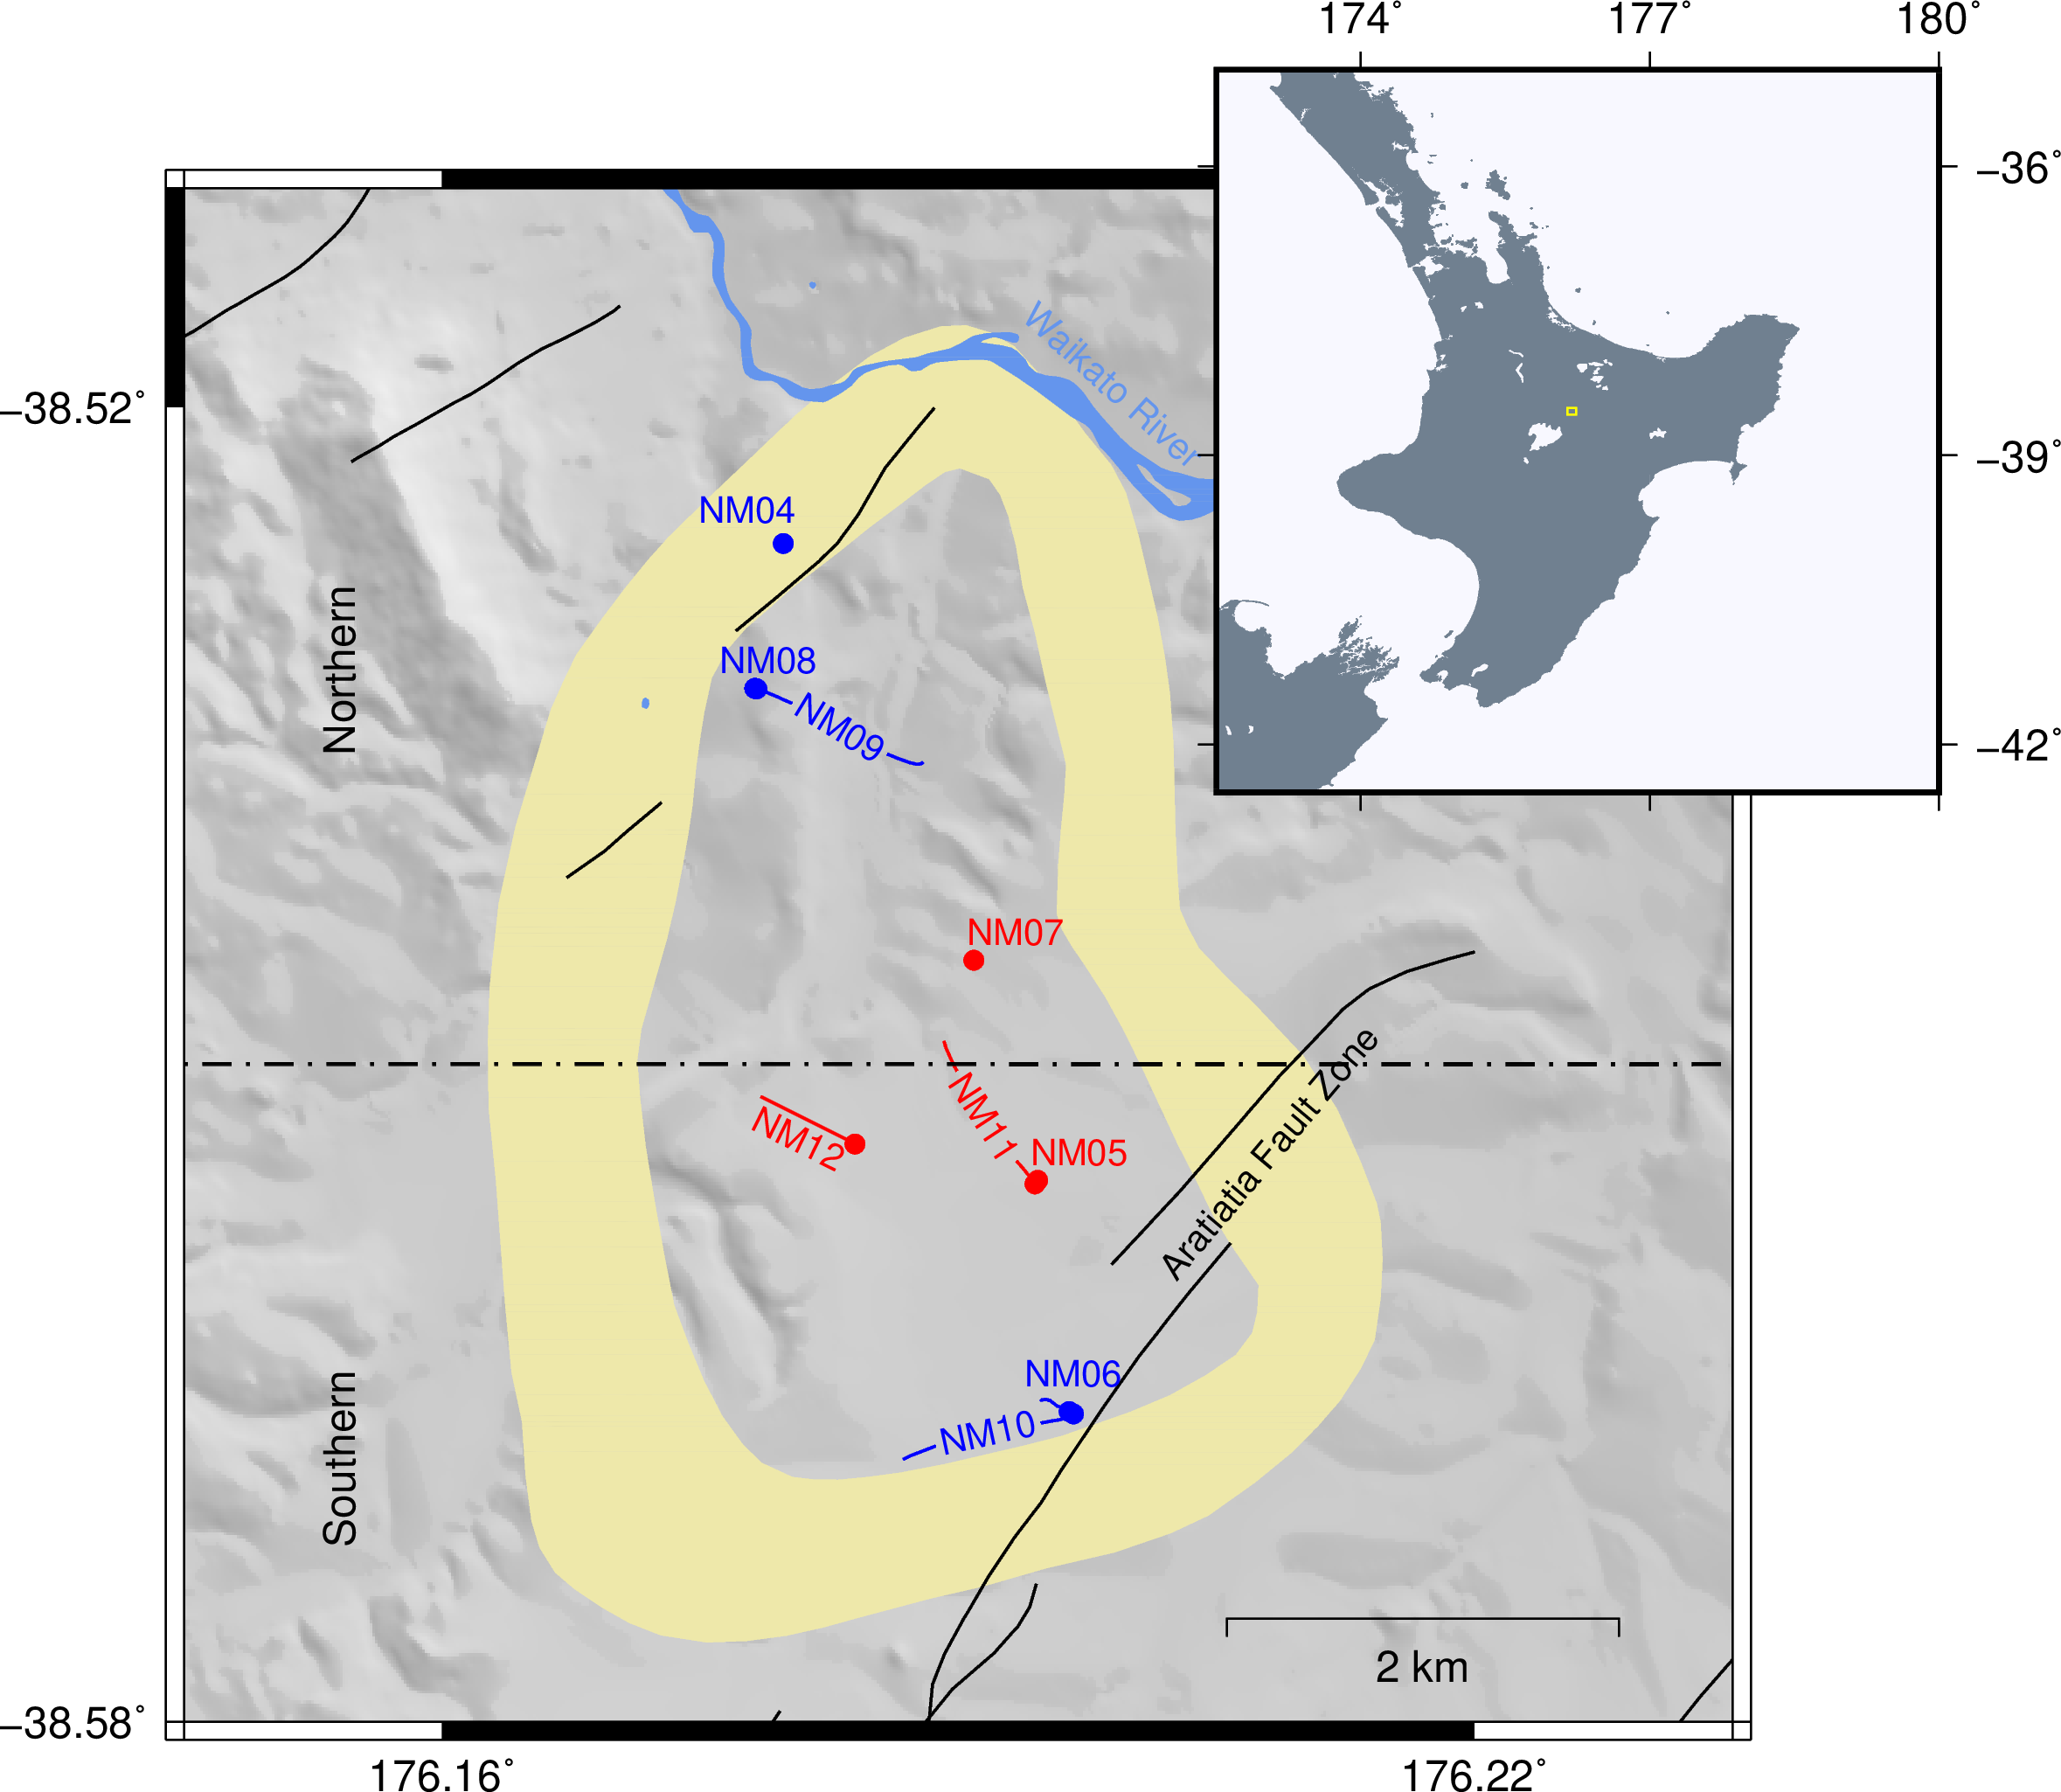
\includegraphics[width=0.70\columnwidth]{Chapter_3_Nga/figures/merc_Nga_overview_temps-wells_12-15/merc_Nga_overview_wells_12-15_original}
\caption{{Overview of the Ngatamariki geothermal field. Injection wells are shown
in blue, production wells in red with dots representing the wellhead and
lines showing the surface projection of the well tracks at depth. Wells
NM04, NM08, NM05 and NM07 are near vertical and, therefore, appear only
as dots in the figure.~ Active faults from the GNS Active Faults
Database~\protect\citep{AFDB} are shown in black. The most likely boundary
of the deep resource as published by~\protect\cite{Boseley_2010} based on
magnetotelluric surveys, is shown in yellow. The northern and southern
portions of the field, as referred to in this work, are divided at
-38.55 degrees latitude and labeled here.
{\label{795275}}%
}}
\end{center}
\end{figure}

\subsection{Mechanisms of microseismicity and permeability enhancement}
The main driver of microseismicity at Ngatamariki is the injection of cool (\textless{100}\textdegree{C}) fluid into the hot ($\sim$280\textdegree C) reservoir. It is generally accepted that fluid injection increases the pore-fluid pressure near an injection well, lowering the effective normal stress and inducing slip on suitably oriented fractures with respect to the local stress field \citep[e.g.][]{Zoback_1997,Ellsworth_2013,Langenbruch_2018}. At every point on a fracture or fault, there is a specific pore pressure increase, $\Delta{P_{crit}}$, that will lower the shear strength of the fracture\slash{fault} to the point of failure \citep{Wiprut_2000}. Injection, especially in high-temperature geothermal reservoirs, also introduces a thermal gradient in the host rock. This may produce enough stress to induce tensile failure or opening of preexisting fractures \citep{Mart_nez_Garz_n_2014}. It also reduces stress locally through thermoelastic contraction of the rock matrix, bringing the reservoir fracture network closer to or further from failure depending upon the direction of fluid flow relative to the orientation of the in situ stress state \citep{Jeanne_2014}. Furthermore, as geothermal fluid moves through a formation, it may dissolve minerals (e.g.\ calcite) out of, or precipitate minerals into, fractures. Though less well understood, this effect may play a large part in creating or destroying permeability through opening or sealing of fractures that would be likely to fail \citep{Clearwater_2015}. Injection and extraction of large quantities of fluid can also significantly change the volume of the reservoir, poroelastically influencing the distribution of stress and often leading to reservoir compaction, surface subsidence and seismicity \citep{Segall_1989,Segall_1998,Bromley_2013}. Finally, slip itself (both seismic and aseismic) transfers stress onto nearby fractures and faults, an effect that has been shown to play a role in triggering subsequent seismicity in geothermal fields and elsewhere \citep{Schoenball_2012,Catalli_2016}.

The relationship between seismicity and permeability has been widely studied in laboratory settings \citep[e.g.][and references therein]{Lee_2002}. When slip occurs on a new or preexisting fracture, asperities become offset and the permeability of that fracture increases (an effect known as self-propping), which depends on the length of the slip vector and the roughness of the fault surface \citep{Ishibashi_2018,Esaki_1999,Fang_2017}. It is commonly assumed that the permeability increase observed during injection is the result of seismic fault slip, a correlation which has been modeled for EGS cases previously (e.g.\ \citet{Baisch_2010}). It is important to note, however, that a large percentage of the permeability enhancement that accompanies well stimulation may be aseismic, as has been directly observed during a decameter-scale injection experiment described by \citet{Guglielmi_2015} and in seismic data recorded during hydraulic fracturing \citep{Das_2011}. Further evidence of aseismic slip has been inferred at the high-temperature Salton Sea geothermal field in southern California from a combined geodetic and seismic dataset \cite{Wei_2015}. \citet{Riffault_2018} have also demonstrated that, in some cases, permeability enhancement may not be coupled to detectable seismic slip at all. In the context of high-temperature geothermal reservoirs, thermal stresses induced near the wellbore may govern most of the permeability enhancement observed during well stimulation through the expansion of permeable zones \citep{grant2013thermal,siega_2014}, a process which may be aseismic.

At Ngatamariki, the dominant processes driving microseismicity have previously been interpreted to be thermal and pore-fluid pressure changes \citep{Sherburn_2015,grant2013thermal}. The Ngatamariki power plant reinjects most of the extracted fluid and, as a result, the pressure drawdown observed across the field is minor ($\sim$0.2 MPa). This suggests that reservoir compaction plays a small role in inducing local stress changes in this case \citep{quinao_2017}. However, at nearby fields that have been produced for much longer than Ngatamariki, significant pressure drawdown-related subsidence has occurred \citep{Allis_2000}. Poroelestic stress transfer resulting from rock matrix contraction and slip on fractures cannot be ruled out as possible factors affecting reservoir permeability and induced seismicity. However, in the case of the NM08 and NM10 injection tests and NM09 Stimulation A (introduced below), the injection of river water also renders unlikely the precipitation of minerals as a possible mechanism of permeability change. This cannot be said of the brine injected during the second phase of NM09 stimulation.

\subsection{Ngatamariki power plant operations} \label{Plant_ops}
Mercury Ltd., then known as Mighty River Power (MRP), began generation of electricity at Ngatamariki in October 2013 with the commissioning of an 82 MWe binary power plant. The company was granted a consent for production of 60,000 tons of geothermal fluid per day, approximately 98\% of which is currently reinjected into the deep reservoir at between 1000 and 3000 m depth. The reinjected fluid is allocated nearly evenly between the injection wells to the north (NM08, NM09) and those to the south (NM06, NM10) \citep{Clearwater_2015,buscarlet_2015}. Between June 2012 and April 2013, three of the four main injection wells were subject to some form of injection operation (Table \ref{table:operations}). Cold-water stimulation of NM08 took place between 8 June and 10 July, 2012 using $\sim$10\textdegree{}C river water. Well NM10 was drilled between late May and early August 2012, using fluid consisting almost entirely of river water, and significant fluid losses occurred after 13 July. After the completion of drilling, NM10 injection testing was conducted on 1--23 September. NM09 was drilled between September and early November 2012, with subsequent injection testing occurring in two phases. The first took place between 14 December 2012 and 4 January 2013 and the second lasted from 13 February to 6 March 2013 \citep{Clearwater_2015}, the latter using geothermal brine instead of river water. This paper focuses on the cold-water stimulation of NM08, drilling and cold-water stimulation of NM10 and cold-water stimulation of NM09.

In March 2013, as the plant was being brought online, Mercury began reinjection of brine into all injection wells including NM06, which had been drilled several years earlier. Geothermal brine at Ngatamariki is injected at a temperature of approximately 90\textdegree C. However, at times when production exceeded plant intake capacity during the early stages of plant startup, some brine bypassed the plant and was injected at temperatures of as much as 150\textdegree C \citep{Clearwater_2015}. Over the following year, injection at Ngatamariki reached a stable level of $\sim$1000 tonnes per hour (t/h) at NM09, $\sim$200 t/h at NM08 and $\sim$800 t/h at NM06. NM10 was initially an active injector but, due to the strong hydraulic connectivity between it and the production well NM05, it was phased out by mid-2015 \citep{buscarlet_2015}.\selectlanguage{english}

\begin{table}
\centering
\resizebox{\textwidth}{!}{%
\begin{tabular}{ccccccc}
    {Operation} & {Zone} & {Start} & {End} & {Injectate} & {Max Q (t/h)} & {Max Pres. (MPa)}\\ \midrule
    NM08 Stimulation  & Northern & 6-8-2012 & 7-10-2012 & River water & 175 & 2.63 (WHP)\\
    NM10 Drilling  & Southern & 5-25-2012 & 8-11-2012 & Drilling fluid & 141 & N/A  \\
    NM10 Stimulation  & Southern & 9-1-2012 & 9-23-2012 & River water & 201 & 9.3 (DHP) \\
    NM09 Stimulation A  & Northern & 12-14-2012 & 1-4-2013 & River water & 170 & 0.2 (WHP); 15.3 (DHP) \\
    NM09 Stimulation B  & Northern & 2-13-2013 & 3-6-2013 & Brine & 152 & 0.3 (WHP); 13.0 (DHP)  \\
\end{tabular}}
\caption{{Table summarizing the injection operations presented here, all of which were undertaken prior to plant startup at Ngatamariki. The maximum pressures reported in the final column are for wellhead pressure (WHP), downhole pressure (DHP) or both where present. Q denotes flow rate in tons / hour.}}
\label{table:operations}
\end{table}

\section{Data} \label{Data}
The Mercury seismic network covers an area roughly 30 km (N--S) by 15 km (E--W) with the bulk of the stations occupying an area 15 km (N--S) by 7 km (E--W) centered around the Rotokawa and Ngatamariki geothermal areas (Figure S1, supplemental materials). The majority of the instruments are either 4.5 Hz Geospace GS-11D short-period geophones or Lennartz LE-3DLite 1 Hz instruments, but the network also includes stations operated by Contact Energy (THQ2, ARAZ) at the Wairakei and Tauhara geothermal fields and nearby stations operated by the national seismic network, GeoNet (WPRZ, PRRZ, HRRZ, ALRZ) (Table T1, supplemental materials). The GeoNet stations are broadband instruments with the exception of WPRZ, which is a 1 Hz LE-3Dlite. From the beginning of 2012 until the end of 2015, the number of operational stations varied between 15 and 29. Sites NS12, NS13 and NS14 in the middle of the Ngatamariki network are 2 Hz borehole instruments installed at depths of between 200 and 514 meters below the ground surface (Figure S1, supplemental materials).

The initial earthquake catalog for this study was provided by GNS Science under contract to Mercury. The waveform data were collected roughly every three months from Mercury's data loggers and supplemented by data from nearby GeoNet stations. GeoNet data were sampled at 100 Hz while the Mercury network data were sampled at 200 Hz. For much of this study, all data were resampled at 50 Hz to reduce computational costs. Events in the initial GNS Science earthquake catalog had been automatically detected and located with the SeisComP3 software package \citep{Weber2007}. We filtered the catalog to include only these events within or immediately adjacent to the field boundaries at Ngatamariki, leaving a total of 1171 microearthquakes of local magnitudes between 0.26 and 3.17. Magnitude distance corrections were computed using events recorded by both the Mercury seismic network and GeoNet. The calibration factor for a given event-station distance, $A_0$ was calculated from $M = \log_{10}A - \log_{10}A_{0}$, where $A$ is the event amplitude at the station and $M$ the GeoNet calculated magnitude. $A_{0}$ was averaged across all stations in the Mercury network for all events recorded by GeoNet to obtain the final calibration factors. A final, static correction factor of +0.32 was applied to the Mercury magnitudes to bring them into agreement with GeoNet-calculated magnitudes (Figure S2). We relocated these events using the double-difference relocation software of \citet{Waldhauser_2000}, the results of which are shown relative to the seismic network in Figure S3 (supplementary materials). Production and injection well locations as well as flow rates and pressures at each well were provided by Mercury.

\section{Methods}
\subsection{Matched filter detection}

The small magnitudes of events, high levels of anthropogenic noise and highly-attenuating geology  at Ngatamariki make detecting microearthquakes difficult. One way to address this difficulty is to use a waveform-correlation-based detection technique. Correlation-based detection, otherwise referred to as matched-filter detection, offers improved performance over traditional, amplitude-based techniques due to its ability to detect signals in noisy data and when multiple events are closely spaced in time \citep{Gibbons_2006, Shelly_2007}. This significantly increases the number of events detected without increasing the rate of false detections and is ideal for monitoring microseismicity. Such a technique is ideally suited to areas of geothermal power generation, which are characterized by numerous noise sources and dense clusters of small seismic events.

Matched-filter earthquake detection relies on waveform cross-correlation of a
known earthquake signal or signals, referred to as templates, with continuously recorded seismic data. The following equation, which we use for this study, describes normalized cross-correlation in the time domain \citep{Chamberlain_2017}:
\begin{equation}
R(x) = \frac{\sum_{x'=0}^{x+w_{x}}(T'(x') \cdot I'(x + x'))}{\sqrt[]{\sum_{x'=0}^{x+w_{x}}(T'(x')^2 \cdot \sum_{x'=0}^{x+w_{x}}I'(x + x')^2}}
\end{equation}
Here $I'$ represents the continuous seismic data of interest and $T'$ represents the template earthquake. $x$ represents the sample in the continuous data between sample $0$ and sample $(N_{x} - w_{x})$, where $N_{x}$ is the length of the continuous data being searched and $w_{x}$ is the length of the template. $x'$ is the position within the window over which the correlation is being calculated.

Each of 1171 events taken from the GNS Science catalog outlined in Section \ref{Data} was used as a template event (Figure S3). Each template consists of one-second-long waveforms, starting 0.1 seconds before the P-phase arrival on the vertical channel at each station on which a P-pick was made (e.g. red waveforms in Figure \ref{971628}). Horizontal channels are not used due to the large uncertainties for the automatic S-picks in the GNS Science catalog. However, a length of one second ensures that both the P- and S-arrival are included in the vertical-channel template for each event due to the short travel times. A length of one second also omits most of the coda, which is incoherent for even highly similar sources. This effect is especially apparent at Ngatamariki, due to the highly-fractured reservoir, large variations in the volcanic geology (i.e.\ welded ignimbrites and ashfall deposits) and surface heterogeneity. After applying an anti-aliasing filter, waveforms were sampled at 50 Hz and filtered from 3.0 to 20.0 Hz to include the high corner frequencies of events with event-station distances of \textless5 km. Continuous seismic data were processed in an identical manner to the templates for the matched-filter routine.

To generate detections, event templates were cross-correlated with continuous
data at a rate of 50 samples per second. At each sample, the cross-correlation
coefficients for each channel of data were summed to create the network detection statistic \citep{Shelly_2007}. A detection was recorded whenever the detection statistic exceeded a threshold value, which in this case was defined as the daily median absolute deviation (MAD) of the detection statistic multiplied by eight \citep[as suggested by][]{Shelly_2007}. We refer to a template event, along with all of its associated detections, as a family.

We split all families into separate groups for northern and southern Ngatamariki
before removing duplicate detections. This allows us to account for simultaneous seismicity within both clusters, which we would expect in response to simultaneous injection at the two distinct injection zones. However, the separation of the two clusters prior to duplicate removal introduces the possibility of double-counting events detected by two templates if both templates are located in separate spatial clusters. We have checked for this case explicitly and have eliminated these cases in the final catalog presented here.

Within each spatial cluster, duplicate removal was conducted by looping through all detections in order of descending detection statistic and removing detections within a user-defined time buffer of two seconds. We adopted two seconds for the time buffer after a visual review of template events revealed
numerous cases of near-repeating seismicity with inter-event times of 3--5 s.

Visual inspection of a subset of the detection waveforms showed that false detections occurred at a rate of approximately 1--3 false detections per day. However, the quantity of detections makes visual review of the entire detection catalog impracticable. Therefore, we employ a sequence of thresholds based on the cross-correlation between the template and detected waveforms to exclude lower-quality events. We do this during both the location and magnitude calculations detailed below. Applying these correlation cutoffs has the effect of suppressing false detections in the final catalog that we use in this analysis. As a final quality assurance step, we visually inspected hundreds of waveforms from the final catalog in order to manually pick first motion polarities and did not encounter a false detection.

\subsection{Detection location} \label{methods_location}
After removing duplicate detections, P-picks for each of the newly detected
events were made at each channel included in the template. For each station, template waveforms were correlated with the detected waveform over a 0.2 second window centered on the detection time. Picks were recorded at the time corresponding to the highest correlation value within that window. However, if the correlation value of the template and detected waveform fell below 0.4, the pick was discarded. We retained all events with more than five picks and discarded those with five or fewer. For the retained events, we then made automatic S-picks \citep{mroczek2016shear} using the method developed by \citet{Diehl_2009} and modified by \citet{Castellazzi_2015}. These events were then located with the nonlinear location program \href{http://alomax.free.fr/nlloc/}{NonLinLoc} \citep{Lomax_2014} using a preliminary 1-D model computed in VELEST \citep{Kissling_1994,sewell2017}(table S1). As a final step, the entire catalog was relocated using the double-difference relocation program GrowClust \citep{Trugman_2017} with differential pick times generated using the Python package hypoDDpy \citep{lion_krischer_2015_18907}. The final double-difference relocations are shown in Figure \ref{827409}.

\subsection{Magnitudes} \label{methods_magnitudes}
To compute the magnitude of the events detected by the matched filter,
we used the method described by \citet{Shelly_2016}. This technique uses pair-wise relative amplitudes between a template event and each of its detections to compute relative moments. This approach computes the relative amplitude, $\alpha$, as
\begin{equation}
\alpha = \frac{v[2]}{v[1]}
\end{equation}
where $v[2]$ and $v[1]$ are the second and first elements, respectively, of the first row of the 2$\times$2 matrix $V'$ in
\begin{equation}
M = U\Sigma V'
\end{equation}
where $M$ is the singular value decomposition of a data matrix containing both the template and the detected waveform on a single channel. The rows of $V'$ are the right singular vectors which map the weight of the left singular vectors, $U$, to the original data vectors. Because the template and detected waveforms in the data matrix are inherently similar, the first left singular vector, $U_0$, should describe only a difference in amplitude between template and detection. The relative amplitude between the two events can therefore be estimated as the ratio of the second and first elements, $v[2]$ and $v[1]$, of the first row of $V'$.

We calculated relative amplitudes only when the cross-correlation coefficient between the template and detection exceeded 0.6 at any given station. Again, we note that template events only contain waveforms for the vertical channels. For those events recorded by a minimum of four stations exceeding the correlation threshold, we calculated the relative moment as the median of the relative amplitudes, following \citet{Shelly_2016}. We note that, because the relative amplitudes are calculated from two waveforms recorded at the same station, there is no need to remove the instrument response.

This approach has proven to be more robust in the presence of relatively dissimilar waveforms than the method of \citet{Rubinstein_2010}, which assumes high correlation coefficients between all events in a family (e.g.\ $\geq$0.85). In the Ngatamariki case, scattering and attenuation effects produce waveforms exhibiting lower degrees of similarity than typical repeating or near-repeating seismicity (e.g.\ along the San Andreas \citep{Rubinstein_2010}).

We used the GNS Science $M_{L}$ (as described in Section \ref{Data}) to calibrate the relative moment calculations from the method above and produce $M_{L}$ estimates for matched-filter detections. This was done by first converting the template local magnitudes to moment magnitudes using the scaling relationship
\begin{equation}\label{ristau}
M_{L} = 0.88M_{w} + 0.73
\end{equation}
determined for locally detected, shallow New Zealand earthquakes \citep{Ristau_2009} and then converting to seismic moment using the equation:
\begin{equation}
M_w = 2/3\log_{10}M_{0} - 9
\end{equation}
\citep{Hanks_1979}. Knowing the relative moment of the template event from the procedure outlined above, we then determined the relationship between the relative moments and actual moment which allowed us to convert relative moments to $M_w$ and then back to $M_L$ using Equation \ref{ristau}.

\subsection{Focal mechanisms and stress inversion}
Focal solutions for selected events were calculated from P-arrival polarities using the Bayesian focal mechanism determination program of \citet{Walsh_2009}. Here, we present only focal mechanism solutions for the 86 events that occurred prior to plant startup in March 2013 and that had sufficiently high signal-to-noise ratio for the arrival polarities to be manually picked. These focal mechanisms were then used to invert for the stress parameters and the direction of maximum horizontal compressive stress (S$_{HMAX}$) within the northern and southern clusters separately, using the methodologies of \citet{Arnold_2007} and \citet{Lund_2007}.

\section{Results}
\subsection{Matched-filter detection}\label{MF-results}
Starting with the 1171 template events in the automatically detected catalog provided by GNS Science, we added 76,286 detections after matched filtering, creating a total catalog of 77,457 detections. At Ngatamariki, seismicity in both the GNS Science catalog and the matched-filter catalog falls into two spatial groups, which we refer to hereafter as the northern and southern clusters. We delineate the templates broadly by latitude whereby the northern cluster contains all templates located north of -38.55 degrees and the southern cluster contains all templates to the south (Figure \ref{795275}). The northern cluster consists of 432 template events, which generated 25,482 detections. The southern cluster consists of 739 template events, which generated 50,804 detections. Two representative detections for a single template from the northern cluster are shown in Figure \ref{971628}.\selectlanguage{english}

\begin{figure}[h!]
\begin{center}
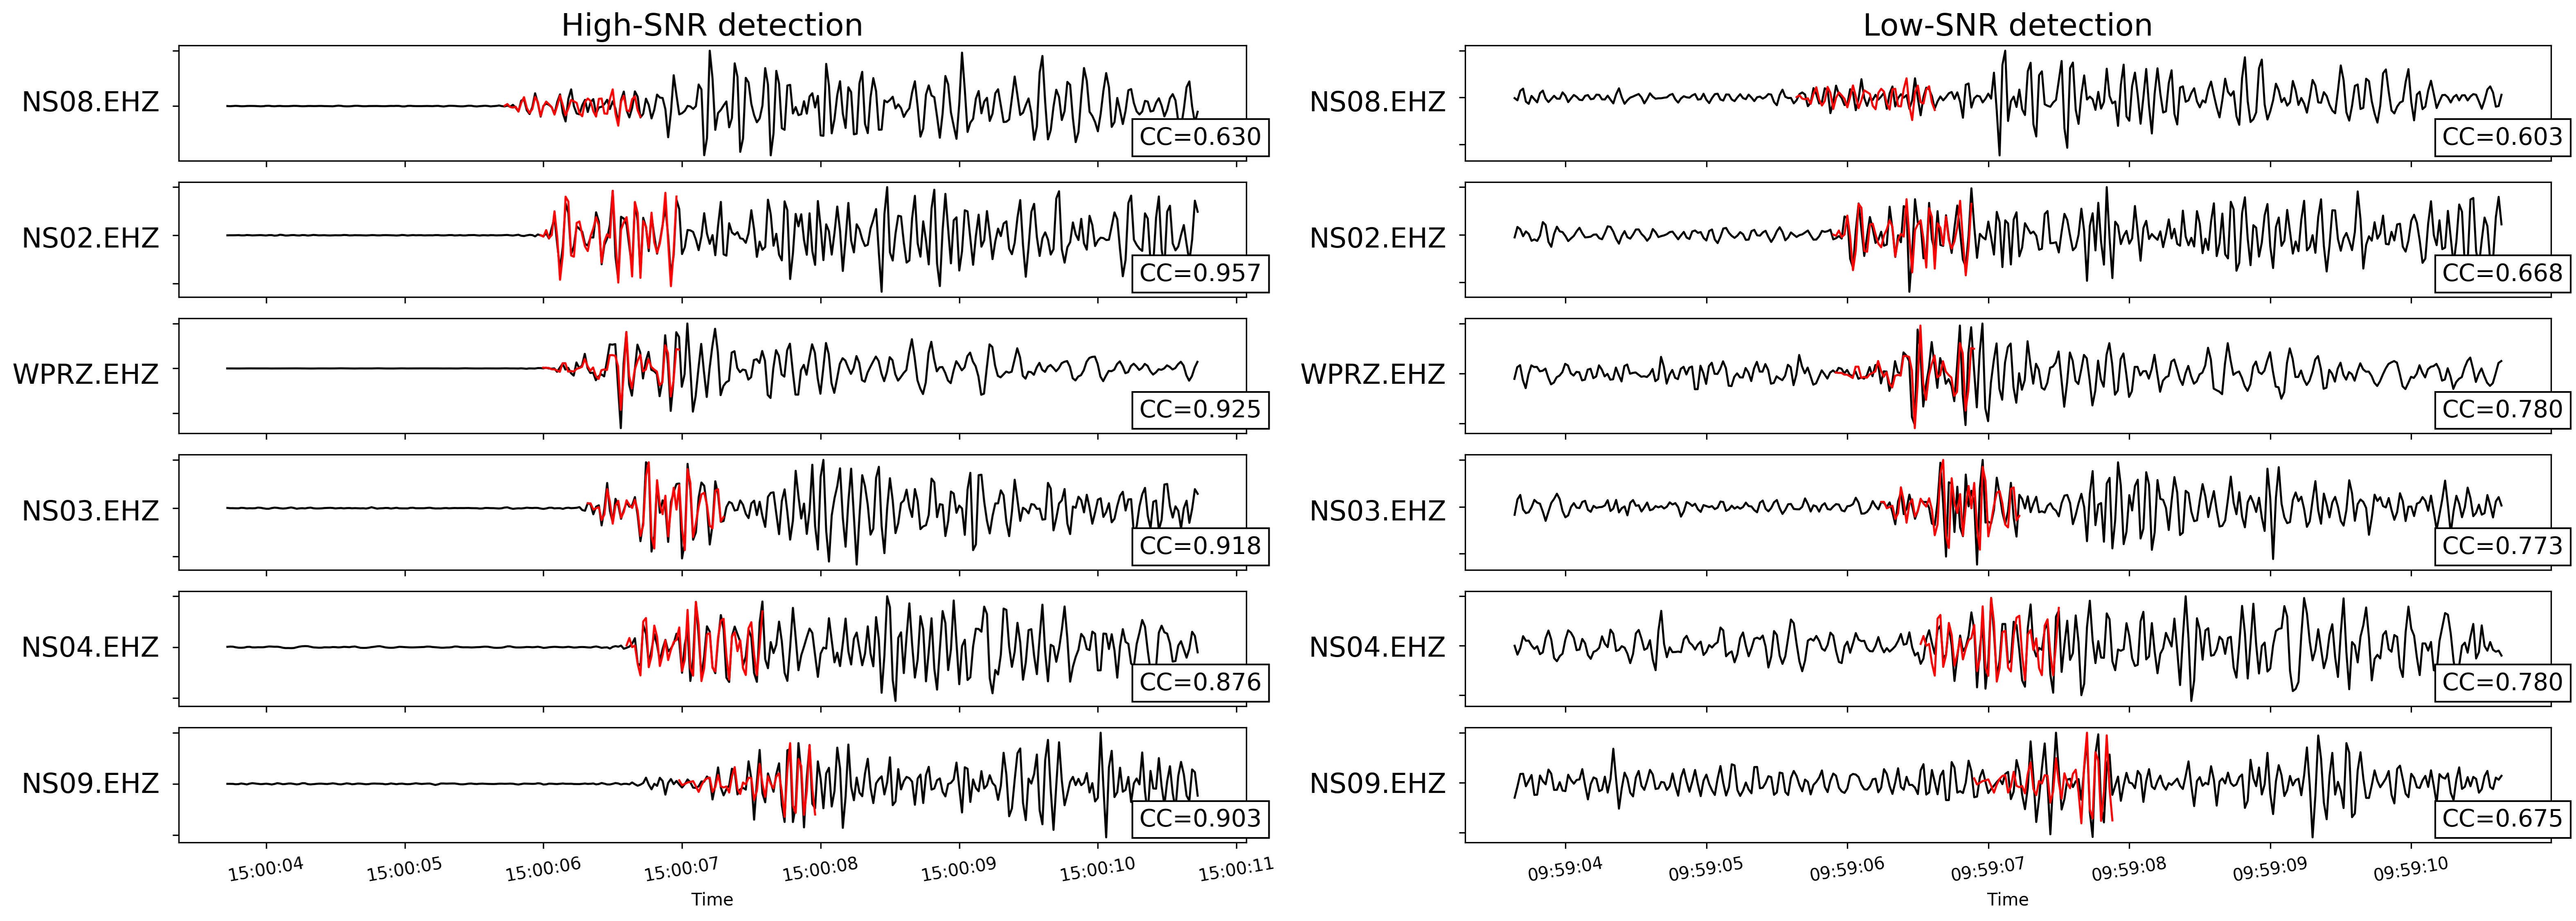
\includegraphics[width=1.00\columnwidth]{Chapter_3_Nga/figures/2012sora453983_20120619_051750460000/det_example_publication_original}
\caption{{Example detections of two events by template 2012sora469246
(signal-to-noise ratio of $\sim$50 and $\sim$3
respectively). The 1 s templates (in red) are overlain on 10 s of
continuous data around the time of detection (black). The
M\textsubscript{L} 0.62 template event occurred on 22 June 2012 and
detected mostly events that occurred during the stimulation of well NM08
between 6 June and early July. The detection on the left represents a
detection of a separate, yet highly-similar, template event (template
2012sora469256) which occurred approximately ten minutes after the
template event shown here. The detection on the right is a
newly-detected event.
{\label{971628}}%
}}
\end{center}
\end{figure}

\subsection{Event location} \label{location_results}
We calculated preliminary locations for 41,114 events of the 77,457 total detections. Of the 5981 of these events for which we calculated magnitudes, we were able to relocate 2554. Given that events detected by the matched-filter method are, by design, similar to the template event that detected them, the locations of the detections should closely match the locations of the template events. Figures \ref{827409} and S3 show the detected and template events, respectively, plotted with depth and colored by their date of occurrence (blue for earlier in the dataset, pink for later).

In northern Ngatamariki, most events occur within a cloud of seismicity extending from $\sim$1500 to 2500 meters below sea level (m bsl). This cloud is spatially coincident with the dominant feedzones in well NM09 at between $\sim$1600--1800 m bsl (Figure \ref{827409}). The injection rate during normal power plant operation is roughly 1100 t/h into NM09 and $\sim$300 t/h into NM08. During the stimulation of NM08, seismicity occurred within a narrow, NW-dipping band at $\sim$2200 m bsl. These events likely define the extent of a suitably-oriented fault that was activated during the treatment and which is discussed in more detail in Section \ref{NM08_stimulation}.

In the south of the field, seismicity occurred in a cluster at depths of $\sim$2000--3000 m bsl, elongated in the NE-SW direction, and sub-parallel to the strike of the Aratiatia Fault Zone (Figure \ref{795275}). These depths coincide with the depths of the major feedzones in injection well NM06, not with the feedzones in NM10. Over the entire four-year dataset, seismicity in the southern injection zone migrates from SW to NE. We attribute this migration to a shift in injection strategy in this part of the field. Originally, injection was split equally between NM10 and NM06, but by 2015 all injection in the south was into NM06 due to rapid returns from NM10 to production well NM05 \citep{buscarlet_2015}.

The depth of seismicity in southern Ngatamariki is greater, on average, than in the north. In the south, hypocentral depths correspond to the depth of the Rotokawa Andesite and the lower Tahorakuri Formation \citep{Chambefort_2014} with shallower seismicity nearer to the production wells than the injection wells. In the north, below $\sim$2000 m bsl, the reservoir is dominated by the intrusive body \citep{Chambefort_2014}. The seismicity depth cutoff near both injection zones is likely related to the depth of permeable zones in the wells \citep{massiot_2012,nm09_report,nm10_report}. In the north, relatively little seismicity occurs within the bounds of the impermeable intrusive body and in the south most events are confined to the Rotokawa Andesite, which is known to be heavily fractured \citep{nm10_report}. The high temperature within the field likely also plays a role in controlling where microearthquakes are able to nucleate. Bottomhole temperatures for the northern injection wells reach $\sim$280\textdegree C and production well NM07 reaches almost 290\textdegree C, approaching the brittle-ductile transition for quartz-bearing rock \citep{Scholz_1988}. In contrast, the maximum temperatures in the southern injection zone reach only $\sim$260\textdegree C and are located away from the main upflow in the field (between NM07 and NM08/09) \citep{Chambefort_2016}. This temperature differential likely governs the difference in the depths of seismicity between the two injection zones, as the host rock should deform brittly to greater depths in the south than in the north.\selectlanguage{english}

\begin{figure}[h!]
\begin{center}
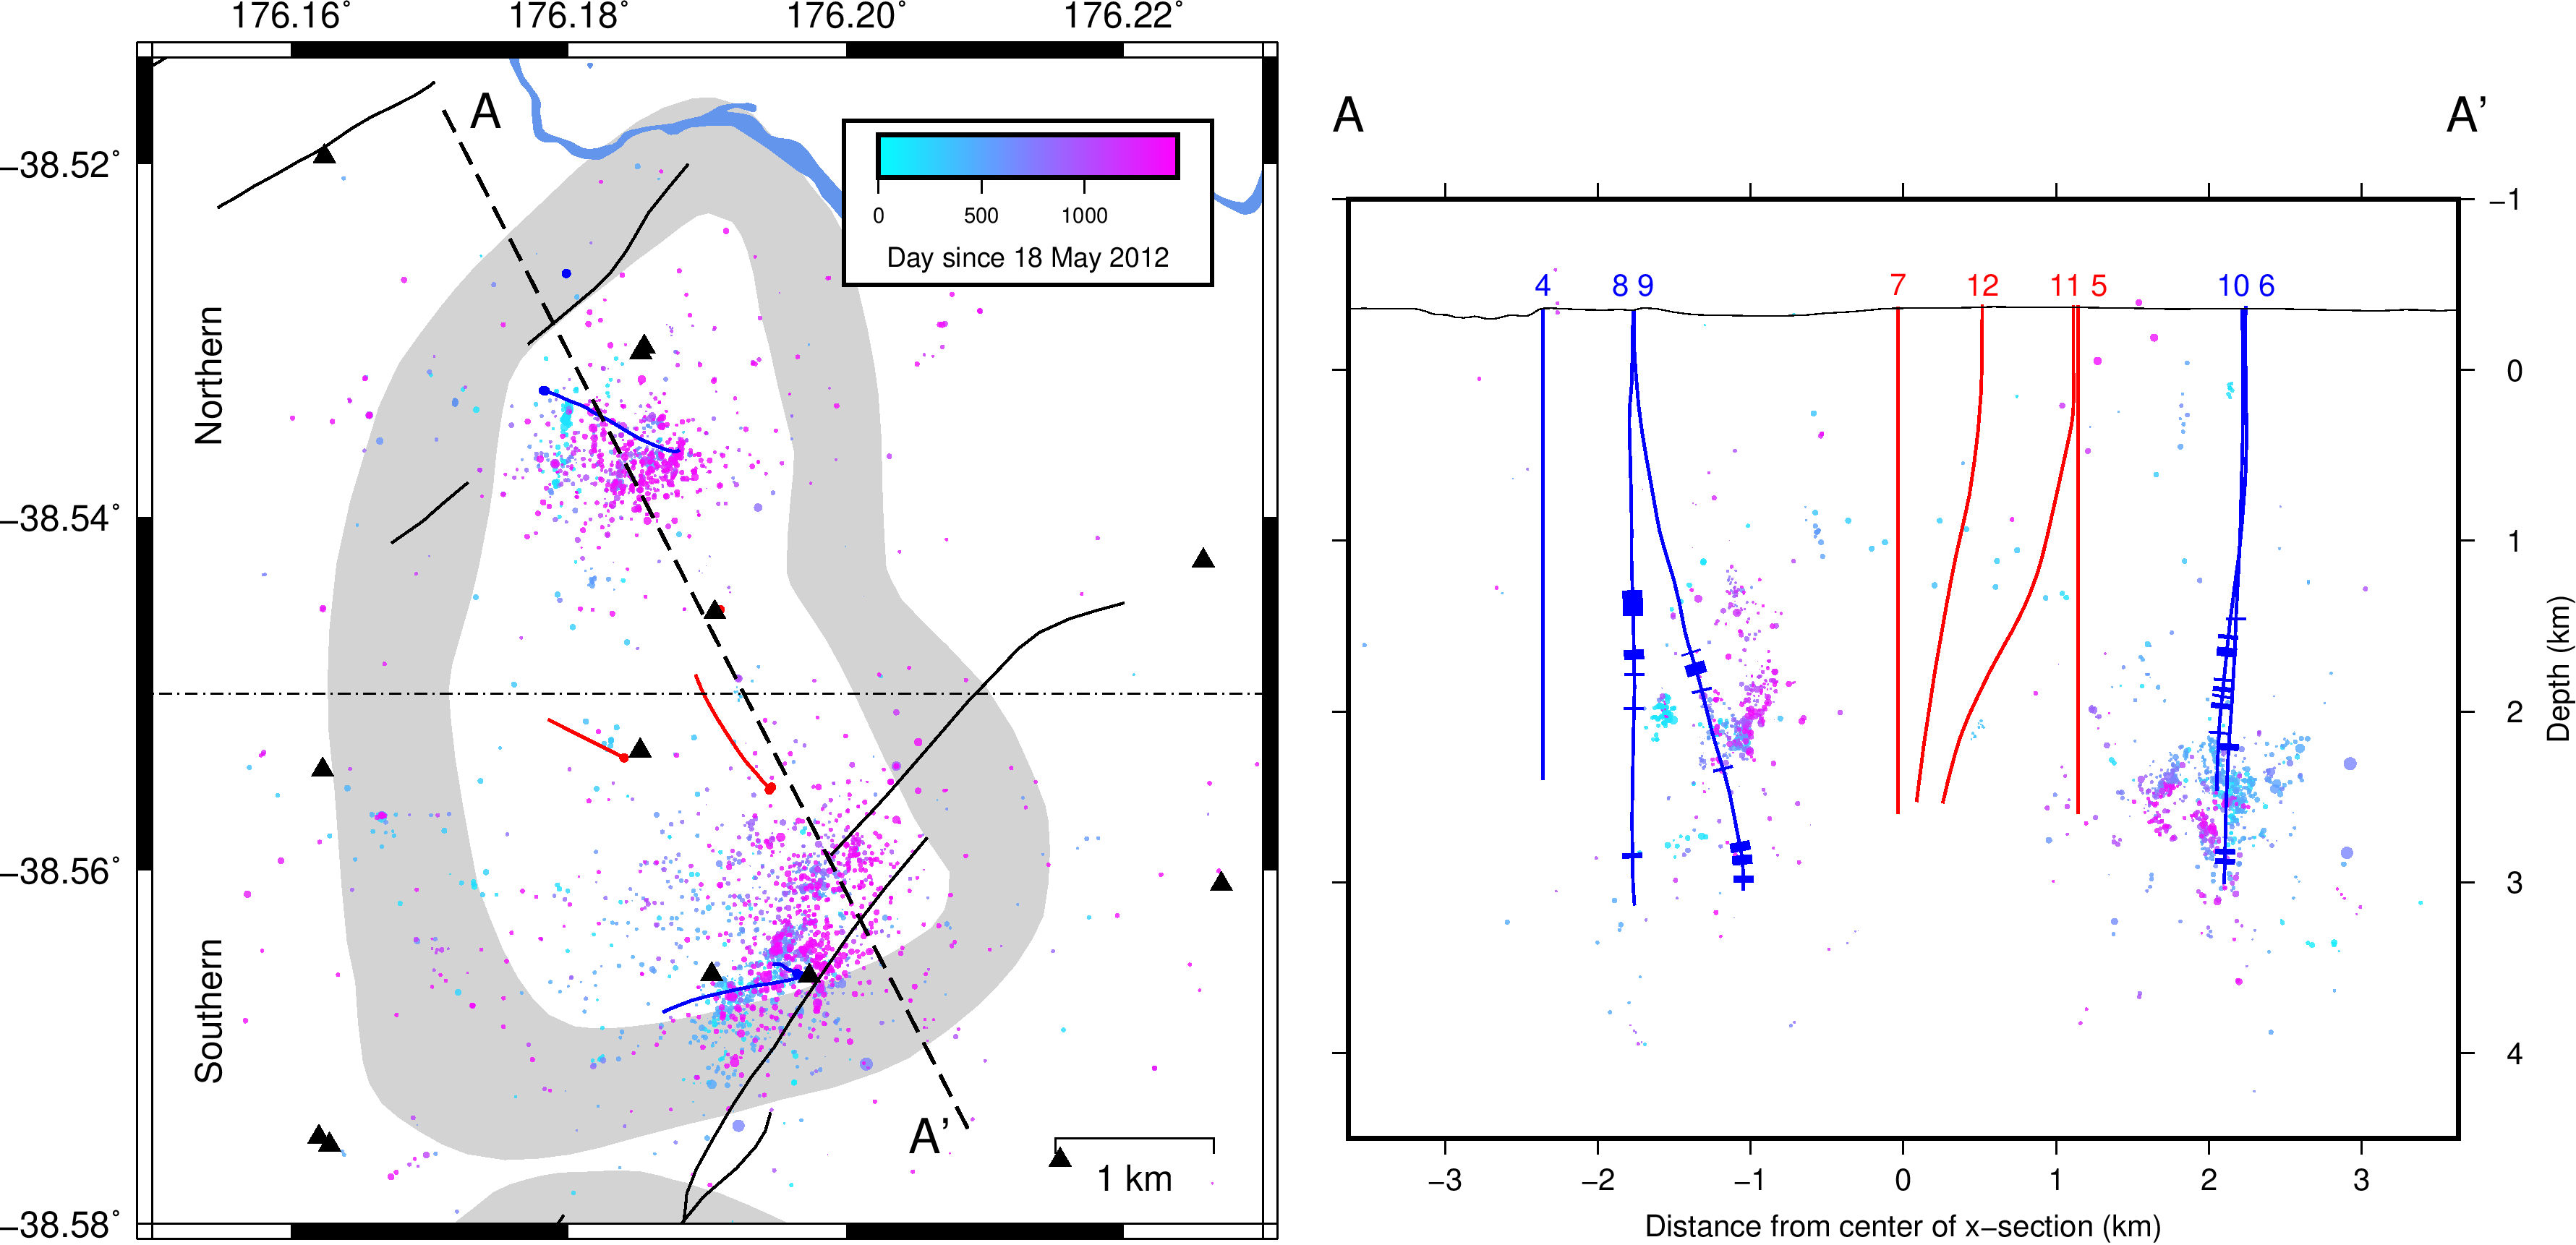
\includegraphics[width=1.00\columnwidth]{Chapter_3_Nga/figures/mrp_hypoDD_Nga_detections_hypoDD/mrp_DD_Nga_dets_GC_11-28-18_original}
\caption{{Relocated Ngatamariki seismic catalog for May 2012 through November of
2015 using the double-difference relocation method
of~\protect\citet{Trugman_2017}. Production (red) and injection (blue) wells are
shown with circles representing the wellhead and lines representing the
surface projection of the wellbore at depth. In cross-section, the major
feedzones in each injection well are shown as wide, blue rectangles.
Events are colored by the date on which they occurred and scaled by
their magnitude (M\textsubscript{max~}= 3.1). Teal corresponds to the
start of the dataset and pink to the end. Black triangles denote
locations of seismic stations. The northern and southern portions of the
field are divided by a dash-dotted line and labelled.
{\label{827409}}%
}}
\end{center}
\end{figure}

\subsection{Magnitude}
We calculated magnitudes for 3725 of the 41,114 located events using the methodology outlined in Section \ref{methods_magnitudes}. This large drop in the number of events is a result of the stringent correlation cut-off imposed ($\geq$0.6 at four or more stations, see Section \ref{methods_magnitudes}), which ensures we retain only high-quality events. Figure \ref{121528} shows the frequency-magnitude distributions for both the GNS Science catalog (dotted lines), constituting the original template events, and the detected events for which we could calculate a local magnitude (solid lines). Here we show the catalog separated into northern and southern clusters. In both clusters, the additional matched-filter detections decrease the minimum magnitude in the catalog to less than zero.

We determine the b-values for the matched-filter catalogs for a magnitude of completeness ($M_c$) calculated using the `maximum curvature' method \citep{Wiemer_1997}. However, we note that, due to the gradual roll-off of these distributions at lower magnitudes (especially for northern Ngatamariki), the `maximum-curvature' estimation method likely underestimates M$_C$ \citep{Wiemer_2000}. Notably, the inclusion of the matched-filter detections does not appreciably lower the magnitude of completeness of the catalogs here, in contrast to what has been shown elsewhere (e.g. \citet{Shelly_2016}). Regardless, the original catalogs were not complete even at higher magnitudes, as suggested by the higher numbers of matched-filter detections for events above $M_L$ 2.0 when compared to the GNS Science catalog.

We suggest that the difference in b-value between the northern and southern clusters (1.84 and 1.20 respectively) reflects a difference in the sizes of fractures and faults that are hydraulically connected to nearby injection wells. The entire field is extensively fractured, as indicated by the available image logs of the injection wells \citep{nm09_report,nm10_report,massiot_2012}, but in the south the active Aratiatia Fault Zone intersects injection wells NM06 and NM10 \citep{nm10_report}. The structures associated with this fault zone may be larger than those in the less-permeable northern portion of the reservoir where active structures are harder to identify \citep{massiot_2012}, allowing for larger-magnitude events to nucleate. During injection operations elsewhere, higher b-values ($\sim$1.5-2.0) have been observed nearer the injection point where high pore fluid pressures can induce slip on fractures subject to low differential stress \citep[e.g.][]{Bachmann_2012}. Slip on these less-stressed fractures may be the explanation for higher b-values at injection sites and volcanic regions \citep{Wiemer_1998}. This may also affect the b-values at Ngatamariki, where WHP in the northern injection zone is consistently $\sim$0.5 MPa higher than in the south.\selectlanguage{english}

\begin{figure}[h!]
\begin{center}
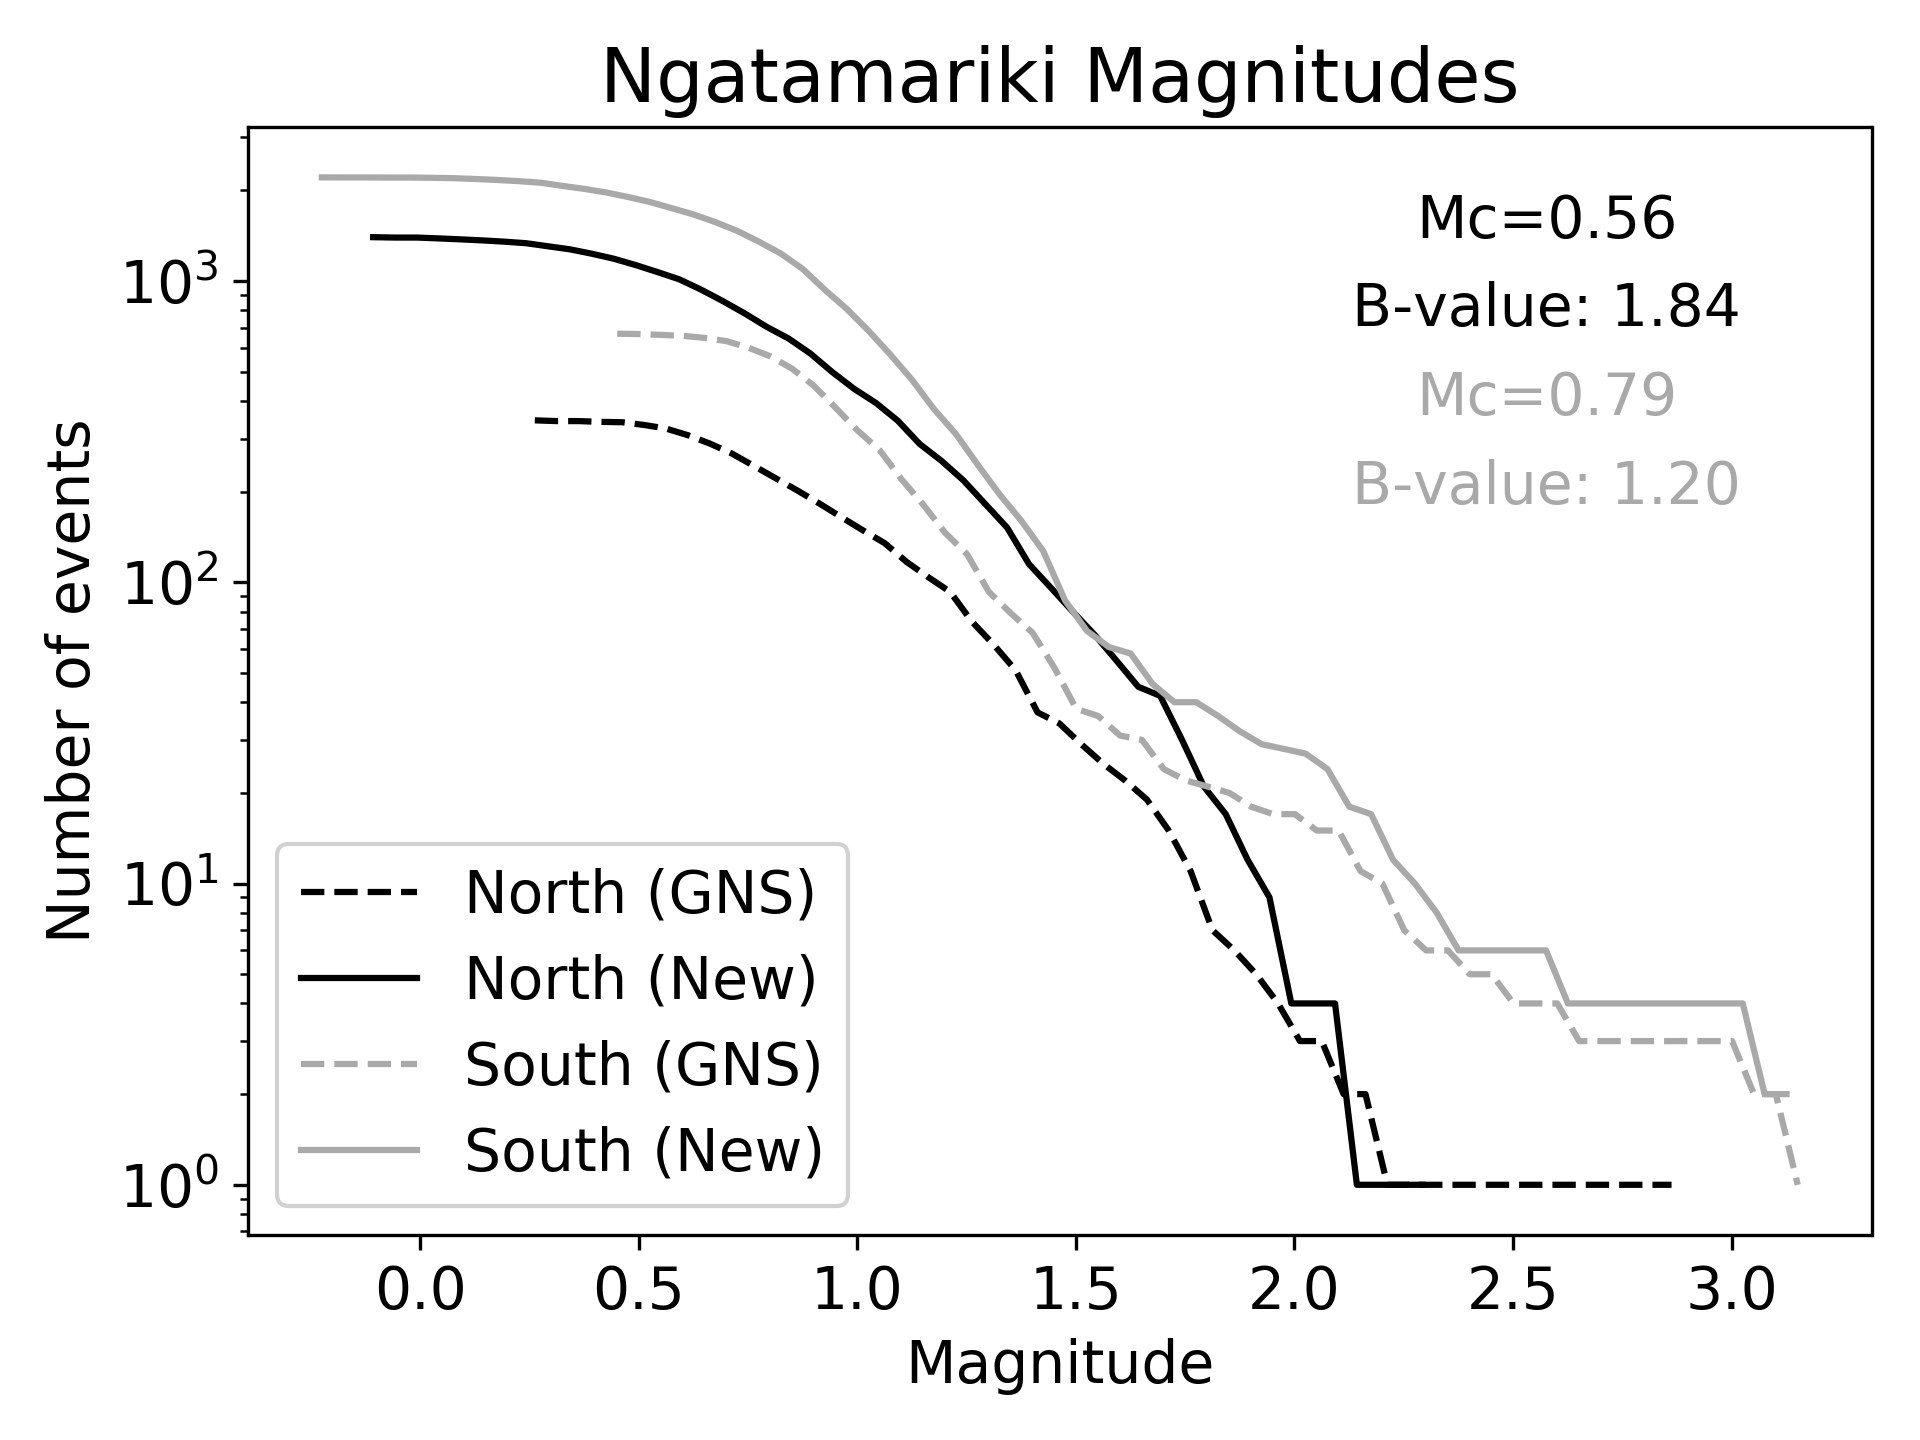
\includegraphics[width=0.70\columnwidth]{Chapter_3_Nga/figures/NgaN_min4_SVD1-5_PCA_mags_vs_temps/Nga_cumulative_bval_plots_combined_12-5_original}
\caption{{Cumulative frequency-magnitude distributions of the GNS Science catalog
of templates (dotted lines) and the final matched-filter catalog (solid
lines) for 2012-2015. Northern and southern Ngatamariki (Nga N, Nga S)
are shown in black and gray, respectively. The magnitude of completeness
is calculated using the maximum curvature method \protect\citep{Wiemer_1997} .
Calculated values of M\textsubscript{C~}and b are noted in the top
right.
{\label{121528}}%
}}
\end{center}
\end{figure}

\section{Discussion}\label{discussion}
Injection wells NM08, NM09 and NM10 underwent injection testing before the commissioning of the Ngatamariki power plant in 2013. These tests provide us the opportunity to study the seismic response to a number of isolated injections without contamination from concurrent injection from nearby wells. Below, we discuss each of these tests in detail and relate the characteristics of the accompanying seismicity to the injection parameters and geology in the respective part of the reservoir. Where possible, we calculate the well injectivity index which we use as a proxy for near-well reservoir permeability \citep{Watson_2013}. Typically, injectivity varies as $t^{n}$ where $t$ is time since the start of injection and $n$ takes a value between 0.1 and 1.0 for most geothermal wells \citep{Clearwater_2015,grant2013thermal}.

\subsection{Northern Injection Zone}
\subsubsection{NM08 stimulation}\label{NM08_stimulation}
Starting on 8 June 2012, NM08 underwent a cold-water stimulation treatment, accepting $\sim$66,000 m$^3$ of water over a period of approximately one month. This was the first injection test in the field and it triggered a sharp increase in the rate of microseismicity, which occurred predominantly in one cluster at the depth of the well's main permeable zone at $\sim$2000 m bsl (Figure \ref{645772}). This sub-planar cluster strikes $\sim$192\textdegree and dips $\sim$66\textdegree, centered on a depth of roughly 2000 m bsl. This is consistent with measurements of fracture orientation made from image logs, which suggest a dominant NE--SW strike for fractures intersecting the well and a dominant NW dip over this depth interval \citep{massiot_2012}. Flow rate, wellhead pressure and injectivity index are shown in Figure \ref{645772}.

Figure \ref{645772} shows the cumulative number of microseismic events during the NM08 stimulation, which included two phases of injection. The first, starting on 8 June, 2012 did not immediately trigger an increase in the rate of seismicity. Instead, there was a period of approximately ten days during which there were no detected events. We interpret this period to correspond to near-field pressurization of the reservoir (NF) followed by pressure breakthrough (BT) to a highly-permeable fracture zone (Figures \ref{645772} and \ref{740510}). This period of testing involved a step-rate injection test in which the WHP response was observed for incremental changes in flow rate. Following this period, on 15 June (middle of BT, Figure \ref{645772}) the injection was changed from a steady-flow to a steady-pressure regime in which flow rate was allowed to vary. This change also corresponded to a modest increase in both the injection rate and WHP. Roughly two days after this change, the rate of seismicity increased to between 5 and 12 events/day in the area of NM08 and this increased rate was maintained until the first phase of injection ended on 26 June (FZ1, Figure \ref{645772}), accompanied by an abrupt halt to seismicity.

Phase two of the stimulation began on 1 July, 2012 (start of RP, Figure \ref{645772}) at slightly higher flow rates than previously ($\sim$150 t/h). Again, the rate of seismicity did not immediately increase once the second phase of injection began. There was a delay of approximately four days before the flow rate was increased to $\sim$175 t/h with an accompanying increase in WHP of approximately 0.5 MPa (FZ2 Figure \ref{645772}). Following this increase, the rate of seismicity increased to 23 events per day (T5), slightly higher than the levels encountered during phase one. This activity ceased as soon as injection was halted on 9 July, bringing the total number of events during the stimulation to 122. The maximum $M_{L}$ during the entire stimulation was 2.1.\selectlanguage{english}

\begin{figure}[p]
\begin{center}
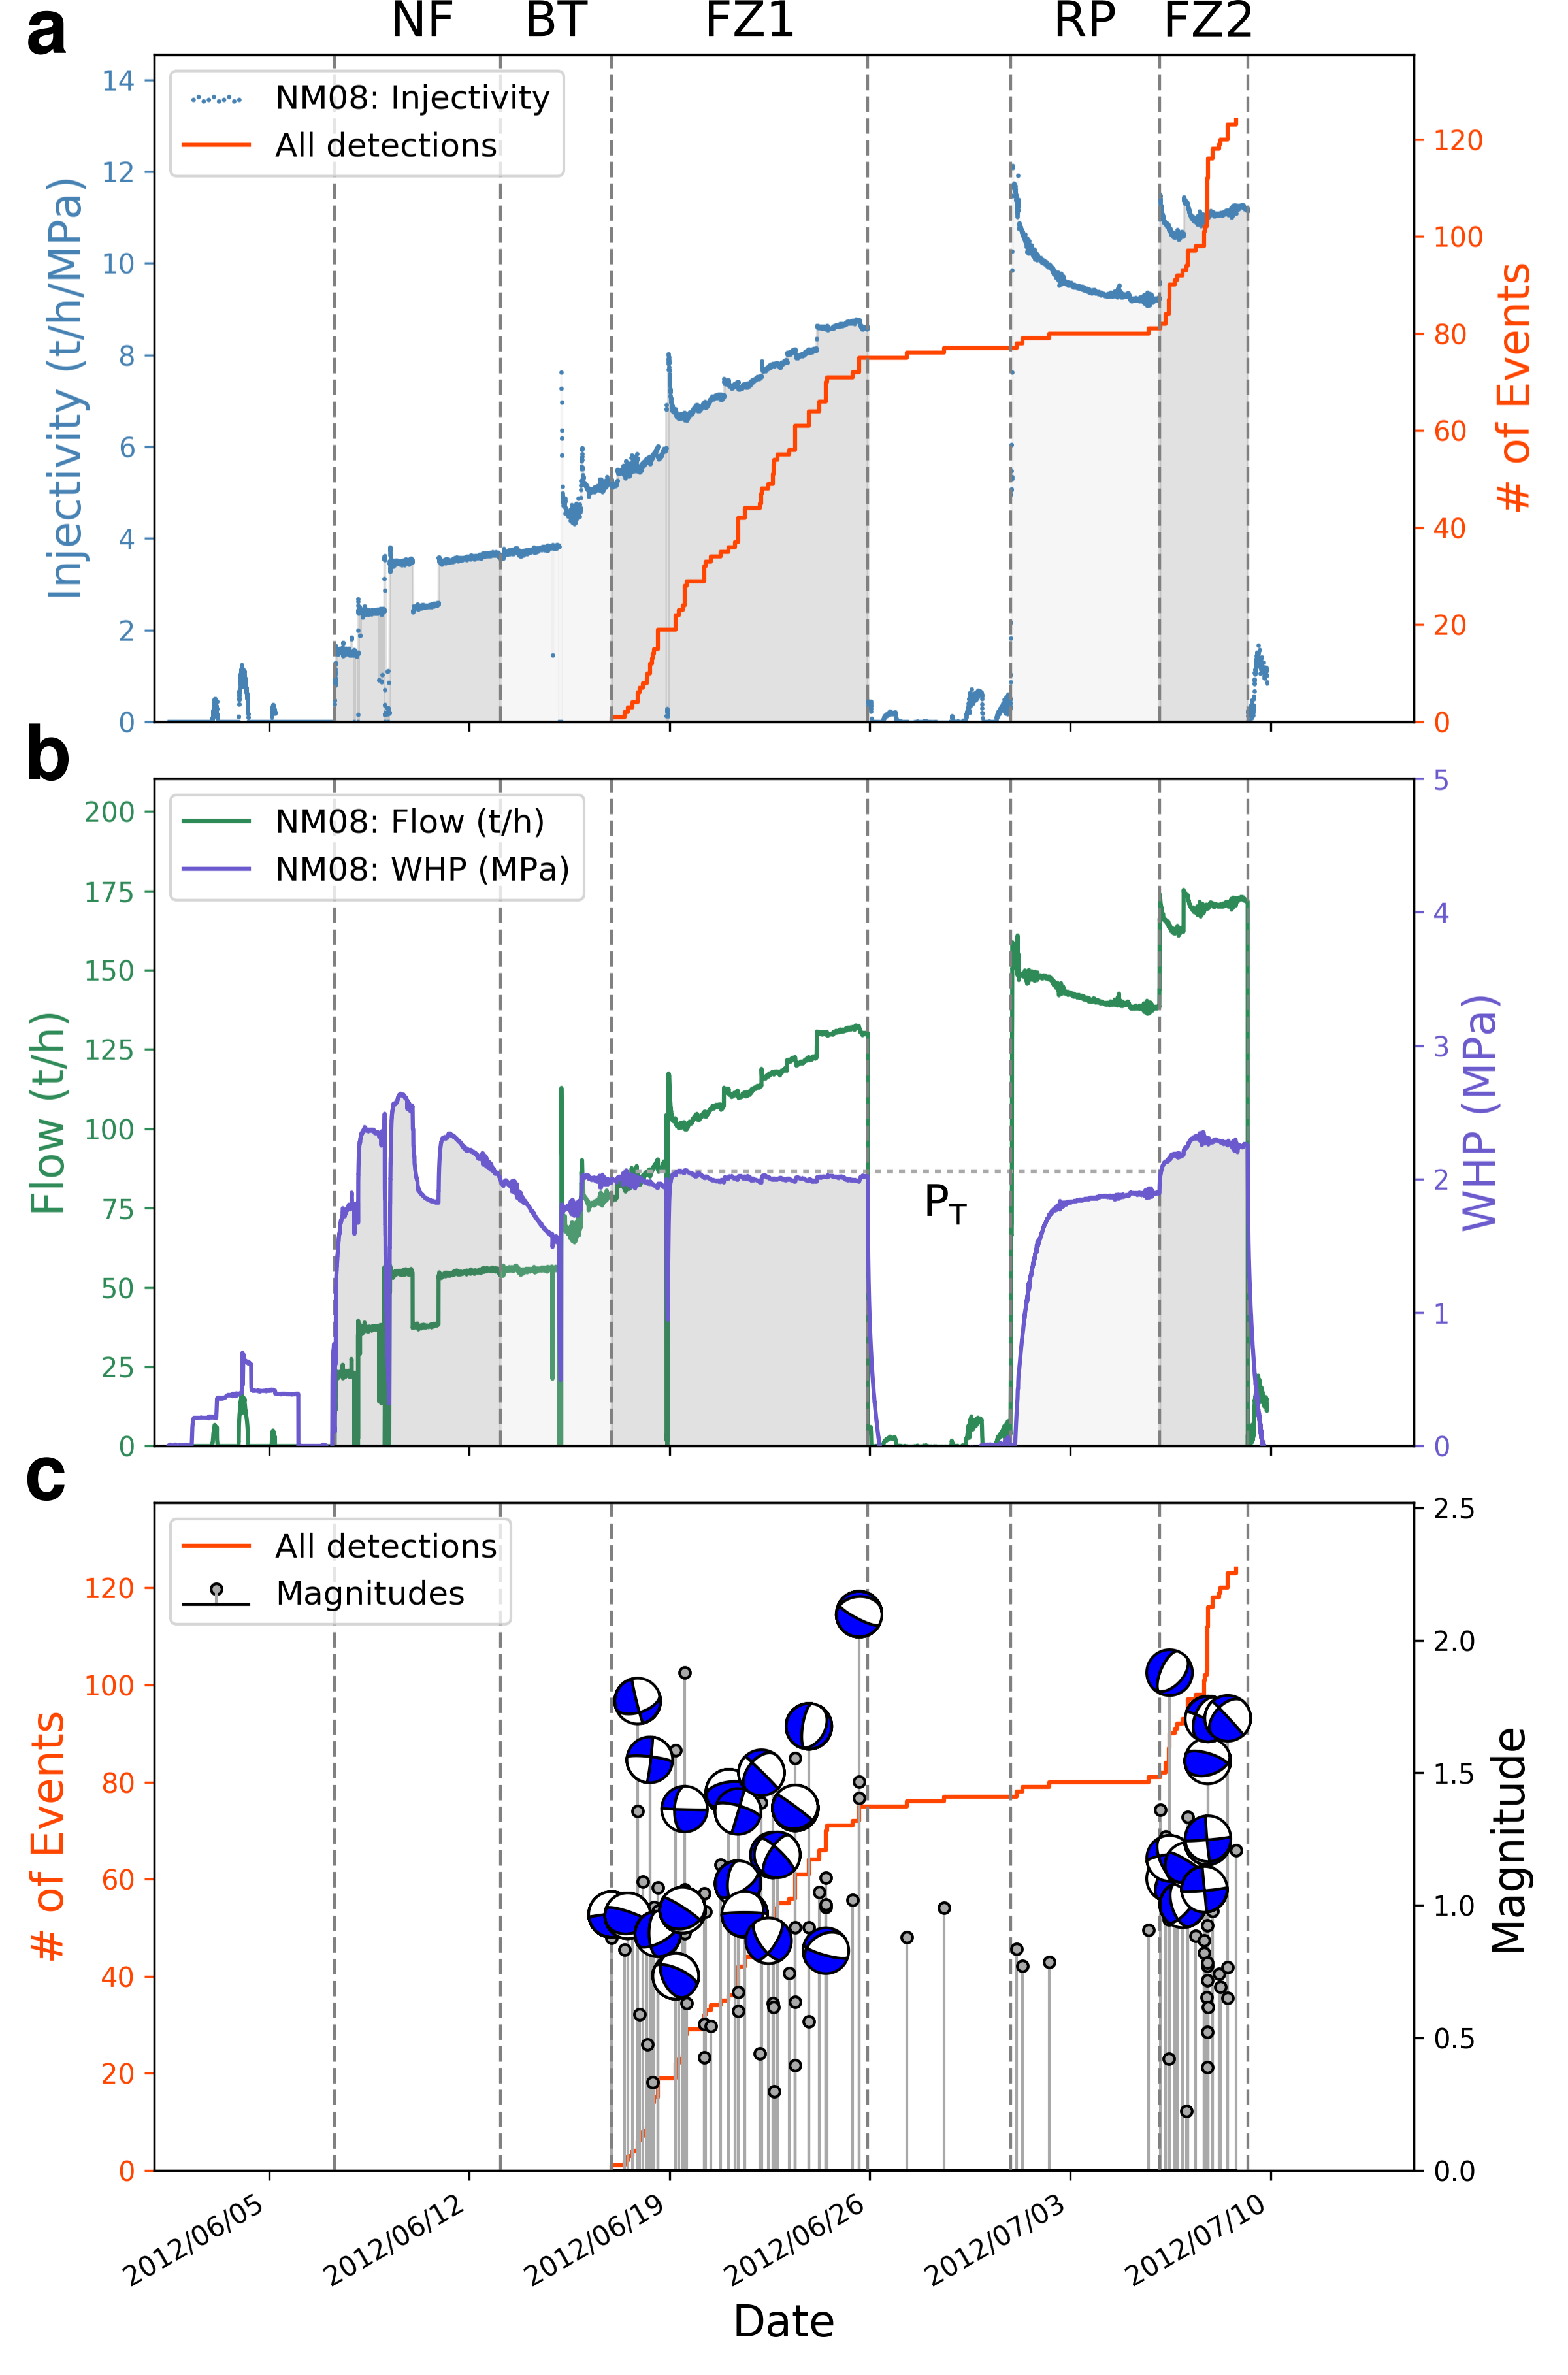
\includegraphics[width=0.84\columnwidth]{Chapter_3_Nga/figures/Multiplet_95_vs_flow_rate/Full_final_cat_flow_WHP_mags_FMs_diffusion_NM08_Stim_II_11-7_GrowClust_no_diffs_lines_gray_labels_12-5_original}
\caption{{Summary of seismicity and injection parameters during the cold-water
stimulation of NM08. A) Cumulative seismicity vs. injectivity index, B)
wellhead pressure vs. flow rate and C)~Local magnitudes and available
focal mechanisms solutions for the stimulation of NM08. Labels at the
top of the plot delineate the following periods of interest: NF:
near-field pressurization of the fracture zones surrounding the dike
swarm, BT: breakthrough of pressurization from the near-well reservoir
to the seismically-active fracture zone, FZ1 and FZ2: fracture zone
pressurization and associated seismicity, RP: renewed pressurization of
the near-well reservoir. Once the fracture zone pore-fluid pressure
exceeds the maximum induced pressure during FZ1 (P\textsubscript{T}),
seismicity is again induced. These periods are detailed in the schematic
in Figure~{\ref{740510}}.
{\label{645772}}%
}}
\end{center}
\end{figure}

Assuming that NM08 is hydraulically connected to a set of fractures, we expect seismicity to occur once an induced pressure-front has reached a critically-stressed subset of fractures in the local stress regime. The advance of the induced pressure front is controlled by the hydraulic diffusivity of the reservoir, which is closely linked to the reservoir permeability. This relationship has led other groups to develop Seismicity-Based Reservoir Characterization (SBRC) to infer diffusivity from the location and occurrence time of induced seismicity \citep[e.g.][]{Shapiro_2002,Shapiro_2009,Parotidis_2004,Jeanne_2015deformation}. At Ngatamariki, and at most other naturally-fractured reservoirs, flow is controlled not by matrix permeability but by the spacing and permeability of fractures \citep{Grant_2011}. If we consider a large enough volume of the reservoir, relative to the fracture spacing, SBRC can be useful in estimating a bulk reservoir diffusivity from the occurrence of seismic events. However, if flow is concentrated in a small number of highly permeable fracture zones (highly anisotropic permeability), as is the case at Ngatamariki, SBRC performs less well in describing reservoir properties. Nevertheless, we have fit a number of curves to the seismicity catalog for each of the injection scenarios detailed in this work (supplemental materials).

The timing and location of seismicity during the stimulation of NM08 provoke a number of questions:
\begin{enumerate}
    \item Why does seismicity lag behind the starts of injection by up to ten days?
    \item Conversely, why does seismicity stop immediately following a halt of injection?
    \item Why are the increase in injectivity index and seismicity poorly correlated in time?
\end{enumerate}

Seismicity trails injection by ten days at the outset of the stimulation, and again by four days at the start of phase two (NF and RP, Figure \ref{645772}). In the first tens of minutes following the start of injection, drilling-related degradation of near-well permeability (i.e. positive skin effects \citep{Grant_2011}) may have contributed to a delayed pressure response between the well and reservoir. However, as the seismic lag time was of the order of days, positive skin effects (normally on the order of hours) cannot account for this observation \citep{horne1995modern}. We propose that the lag is due to geologic heterogeneity in the Tahorakuri volcaniclastic succession that hosts the reservoir, which defines where the permeable zones of the well are located, as well as the orientation of the fracture network.

The main permeable zone of NM08, which coincides with the depth of seismicity during stimulation, is defined by a series of mafic dikes or sills \citep{Chambefort_2014,massiot_2012} (Figure \ref{740510}). Image log quality at this depth is poor, and the orientations of these dikes is poorly constrained \citep{massiot_2012}, but their emplacement orientation is likely to have been controlled by the prevailing stress field 0.64--0.79 Ma \citep{Chambefort_2014} and related to the emplacement of the tonalite intrusive at the bottom of the well (Figure \ref{740510}). If we assume that flow is concentrated within the damage zone surrounding the dikes and/or within the dikes' internal structures (such as cooling joints or flow bands \citep{Massiot_2017}), it may be that these structures are not optimally oriented for failure in the current stress regime. Although the prevailing tectonic environment during emplacement of the intrusive was similar to that of the present (i.e.\ active rifting \citep{Wilson_2016}), highly active volcanism in the TVZ, including the subsequent formation of the adjacent Whakamaru caldera (0.35 Ma), would likely have modified the Ngatamariki stress state \citep{Wilson_1995}.

We hypothesize that initial flow from NM08 was concentrated in these non-critically-stressed dike-related structures, and therefore did not trigger detectable seismicity (NF Figures \ref{645772}, \ref{740510}). In this case, the time lag in seismicity corresponds to a period of near-field pressurization during which NM08 was not hydraulically connected to the fracture zone defined by the hypocenters in Figure \ref{532034} (striking 192\textdegree, dipping 66\textdegree NW). If we consider an alternative scenario, in which NM08 was always hydraulically connected to the fracture zone, then we would expect seismicity to have been triggered by the diffusion of the maximum observed WHP to the fracture zone (2.6 MPa during NF, Figure \ref{645772}). However, this scenario is unlikely in view of the immediate shutoff of seismicity when the well was shut-in, which would imply hydraulic diffusivities an order of magnitude greater than those required by diffusion of the maximum WHP to the fracture zone. We discuss this in more detail below.

We infer that, during the near-field phase (NF), a small set of near-field fractures was pressurized, with a maximum measured wellhead pressure of 2.6 MPa (the highest WHP measured at Ngatamariki to date). Seismicity was induced in the fracture zone (roughly 200 m from NM08) during a period of constant 2.0 MPa WHP (FZ1, Figure \ref{645772}). The hydraulic connection to the fracture zone would need to have been established while the WHP was below this $\sim$2.0 MPa threshold, otherwise seismicity would have been induced earlier. The degree to which the fracture zone was critically stressed may also explain a part of the time lag during what we call `breakthrough' (BT, Figure \ref{645772}), as it may have taken time for the pressure perturbation to reach the value, $\Delta{P_{crit}}$, at which it induced slip.

A common observation during injection operations worldwide is post-injection, persistent seismicity \citep[e.g.][]{Fehler_1998,Rutledge_2003,Shapiro_2002}. Many of the largest injection-induced events have occurred after shut-in of the injection wells in question \citep[e.g.][at Basel]{Mukuhira_2017}. At Ngatamariki this was not the case, as near-well seismicity ceased with the halt in injection for both phases of the NM08 stimulation (end of FZ1 and FZ2, Figure \ref{645772}). Assuming an unbounded reservoir, the relaxation of the shut-in-induced pressure perturbation is also a diffusive process (termed the `back-front' of seismicity by \citet{Parotidis_2004}). In the NM08 case, an immediate cessation of seismicity on shut-in would imply nearly infinite reservoir permeability between the well and the seismically active zone. This is incompatible with flow through the reservoir rock matrix, which has a calculated in-situ permeability of $~6\times10^{-18}$m$^2$ \citep{Cant_2018}, but could occur if the effective reservoir permeability is controlled by fractures. If we conceptualize the set of fractures connecting NM08 to the active fracture zone as a series of pipes with effectively infinite permeability, then a pressure perturbation applied at one end produces a near-instant pressure response on scales of 100s of meters (the so called `water hammer' effect \citep{Ghidaoui_2005}). The fracture network at Ngatamariki would have sufficient permeability to transmit these pressure perturbations rapidly to distances of 100s of meters, far enough to reach the seismically active zone. Once a drop in pore fluid pressure has propagated to the critically stressed fracture zone ($\sim$ 200 m from NM08), seismicity should cease. We suggest that in order for the initial time lag and eventual rapid halt in seismicity during NM08 stimulation to coexist the hydraulic conductivity between NM08 and the seismically active fracture zone must have been established during the injection (during BT, Figure \ref{645772}).

Injectivity gain and seismic slip during the stimulation of NM08 are not well correlated. During phase one of injection (NF, BT and FZ1), injectivity increased significantly ($n=$0.6-0.7, where injectivity increases as $t^n$ for geothermal wells \citep{Clearwater_2015,grant2013thermal}, indicating that near-well permeability was increasing. However, during near-field pressurization (NF), no seismicity was detected, suggesting that the initial permeability enhancement resulted from aseismic processes as has been observed elsewhere \citep[][and references therein]{Cornet_2016}. The rate of injectivity increase was also insensitive to the eventual onset of seismicity on 17 June (FZ1, Figure \ref{645772}). \citet{Guglielmi_2015} measured three-dimensional fault displacement (with $\mu$m accuracy) and estimated permeability enhancement during the initial stage of a decameter-scale injection experiment, showing that most of the estimated permeability gain was a result of fault-normal displacement and not shear slip \citep{Guglielmi_2015}. While the temperature contrast between the injection fluid and reservoir was negligible for their experiment, we propose that a similar period of fracture-normal, aseismic displacement occurred during the drilling and subsequent stimulation of NM08. The large temperature contrast between injected fluid and reservoir rock at Ngatamariki (up to $\sim$226\textdegree C) served to encourage fracture-normal displacement as a result of thermal contraction of the fracture walls. As suggested by \citet{stephens1982hydraulic}, the thermally-induced circumferential stress at the wellbore is \cite{zoback2010}:

\begin{equation}
\Delta\sigma_{T} = -\frac{\alpha_{L}E\Delta{T}}{1 - \nu}
\end{equation}

with $\alpha_{L}$ being the coefficient of thermal expansion of reservoir rock, $E$ the Young modulus, $\Delta{T}$ the temperature difference between reservoir rock and injectate and $\nu$ Poissons ratio. We assume $\alpha_{L}=1\times10^{-5}$K$^{-1}$ \citep{Bauer_1983}, $E = 20\times10^{9}$Pa \citep{Cant_2018}, $\nu = 0.25$ and a temperature difference of 204\textdegree C (interpreted from pressure-temperature spinner data at feedzone depth during stimulation). This yields a thermal stress at the wellbore of approximately --54 MPa. Understanding the direction and rate of flow is necessary to interpret how such thermal stresses would affect the effective stresses acting on a set of fractures. As we do not know the predominant flow direction, especially within and around the dike swarm, we cannot comment on the effect on the criticality of the fractures. However, the lack of seismicity suggests that such cooling effects may have stabilized the fracture network as was modeled by \citet{Jeanne_2015tensor}.

The thermal diffusivity of the reservoir matrix is typically orders of magnitude lower than the effective hydraulic diffusivity of the reservoir (mm$^2$/s and m$^2$/s, respectively) \citep{Kanamori_1968,Shapiro_2002}. Nevertheless, these thermal effects likely dominate the increase in well permeability at NM08. This model of thermal-expansion-driven stimulation has been proposed by \citet{grant2013thermal} and \citet{siega_2014}, who tested it against a number of geothermal injectivity datasets in New Zealand and elsewhere. Self-propping of slipping fractures, which is associated with seismic slip, is also known to increase fracture permeability \citep[e.g.][]{Lee_2002}, and this process undoubtedly influences the permeability of the seismically active fracture zone. However, the injectivity increase as measured at the well appears to be far more sensitive to other processes, which we suggest is dominated by near-well thermal contraction of the fracture network walls.

Phase two of NM08 stimulation was also accompanied by a time lag (this time of four days) prior to the response of seismicity. In this case, the lag corresponds to the time until the previous highest pore-pressure perturbation (P$_T$, Figure \ref{645772}) was exceeded. This behavior is often referred to as the Kaiser effect \citep{Holcomb_1993}. Assuming that hydraulic connectivity from NM08 to the active fracture zone was not established until the `breakthrough' period (BT, Figures \ref{645772}, \ref{740510}), the highest pressure perturbation to which the fracture zone was subjected during the period of seismic slip corresponded to a WHP of roughly 2 MPa. As soon as WHP exceeded this 2 MPa threshold during phase two, seismicity restarted. This reinforces the interpretation of a high permeability fracture network within 200 m of NM08 following the near-field (NF) and breakthrough (BT) of phase one (Figure \ref{645772}).\selectlanguage{english}

\begin{figure}[h!]
\begin{center}
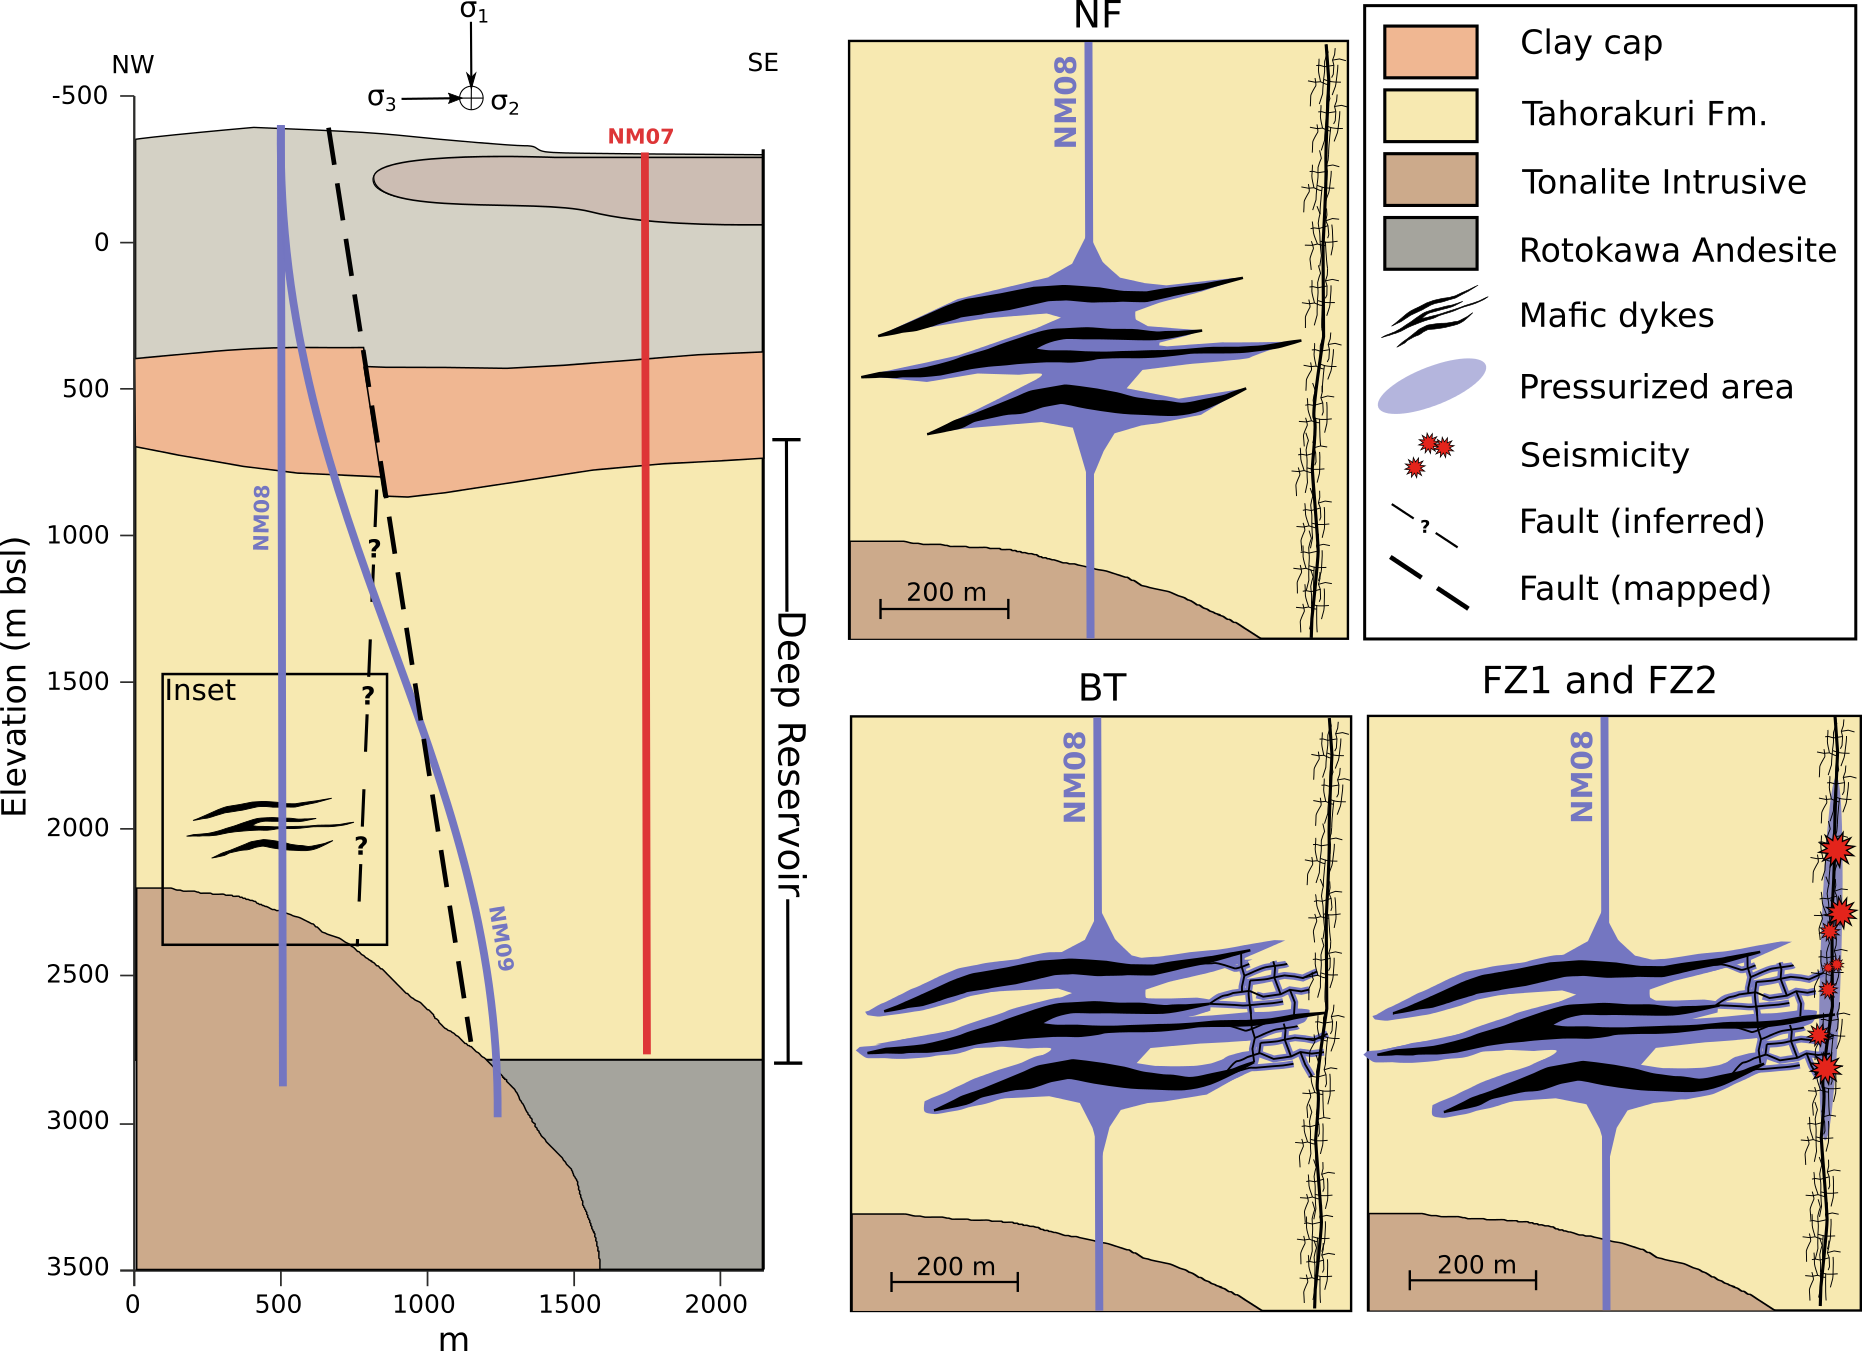
\includegraphics[width=1.00\columnwidth]{Chapter_3_Nga/figures/NM08_stimulation_cartoon/NM08_stimulation_cartoon_original}
\caption{{Schematic illustrating the sequence of events occurring at depth during
NM08 stimulation. The headings of the inset panels correspond to the
periods labeled at the top of Figure~{\ref{645772}}.
The main permeable zone in well NM08 corresponds to a depth where the
well intersects a mafic dike swarm. During NF, hydraulic conductivity
between NM08 and the soon-to-be-active fracture zone was low. This
period corresponds to a pressurization of the small, near-well fracture
network hosted in and around a set of mafic dikes, hence the relatively
high WHP but lack of seismicity. During BT, while WHP was below 2 MPa, a
hydraulic connection was established with the fracture zone, consistent
with increasing injectivity at the well. During FZ1, once WHP was
increased to a steady 2 MPa, the pressure perturbation was able to
diffuse into the fracture zone, weaken suitably oriented fractures and
generate seismicity. At the start of phase two, the fracture network
repressurized until it reached the maximum pressure encountered during
phase one, at which point seismicity recommenced (FZ2).
{\label{740510}}%
}}
\end{center}
\end{figure}

\subsubsection{NM09 injection testing}
Injection well NM09, in the north of the field, underwent two periods of injection prior to plant startup (supplements), accepting $\sim$56,000 m$^3$ of water between 13 December, 2012 and 4 January, 2013 and $\sim$60,000 m$^3$ of geothermal brine between 12 February and 6 March, 2013. The second of these tests used geothermal fluid injected directly from the plant ($\sim$90\textdegree{C}), and not river water ($\sim$10--20\textdegree{C}) as was injected at NM08, meaning that the degree of thermal contraction of the near-wellbore fracture walls was likely less than during the first portion of the NM09 test or at NM08. If we perform the same calculation for circumferential (hoop) stress as done previously for NM08, but with a $\Delta{T}$ of 120\textdegree C, instead of 204\textdegree, we get a thermally-induced stress of --32 MPa, or $\sim$60 \% of the stress induced by cold-water stimulation. Only 11 seismic events were detected within the reservoir during both phases of NM09 stimulation combined. Given that NM08 and NM09 were drilled in the same part of the reservoir, the difference in seismic response is surprising. However, \citet{Clearwater_2015} pointed out that there are major structural differences between NM09 and NM08, despite their proximity. NM08 was drilled directly into the low-permeability intrusive body in this section of the field, whereas NM09 is deviated and was completed in the intrusive's highly-permeable damage zone. Importantly, image logs reveal that NM09 intersects a number of highly-permeable fault zones at depths of $\sim$1850--2300 m bsl \citep{nm09_report}, which were not intersected by NM08. During reservoir tracer testing, it was also shown that NM09 is better-connected to the production wells than NM08 \citep{buscarlet_2015}. This implies a degree of compartmentalization in the northern reservoir, with the structure delineated by the NM08 seismicity possibly acting as a cross-strike flow barrier \citep{buscarlet_2015} (Figure \ref{532034}).

The high-permeability feedzones at NM09 inhibit pressure buildup in the reservoir during injection. During the injection tests, WHP at NM09 never exceeded 0.1 MPa and was often zero, implying that fluid entered the reservoir under its own weight, thereby decreasing the likelihood of inducing seismicity through pore-pressure diffusion. However, injectivity increased in the absence of seismic slip (n=$\sim$0.4--0.6) \citep{Clearwater_2015}. As at NM08, this observation indicates that permeability was enhanced through undetected (small) seismic slip, aseismic slip\slash{opening} of permeable zones connected to the wellbore, or both. It also reveals an even stronger decoupling of injectivity and near-well seismicity than at NM08, with the observed gain likely a result of thermoelastic stresses near the wellbore, especially during cold water injection in phase one.\selectlanguage{english}
\begin{figure}[h!]
\begin{center}
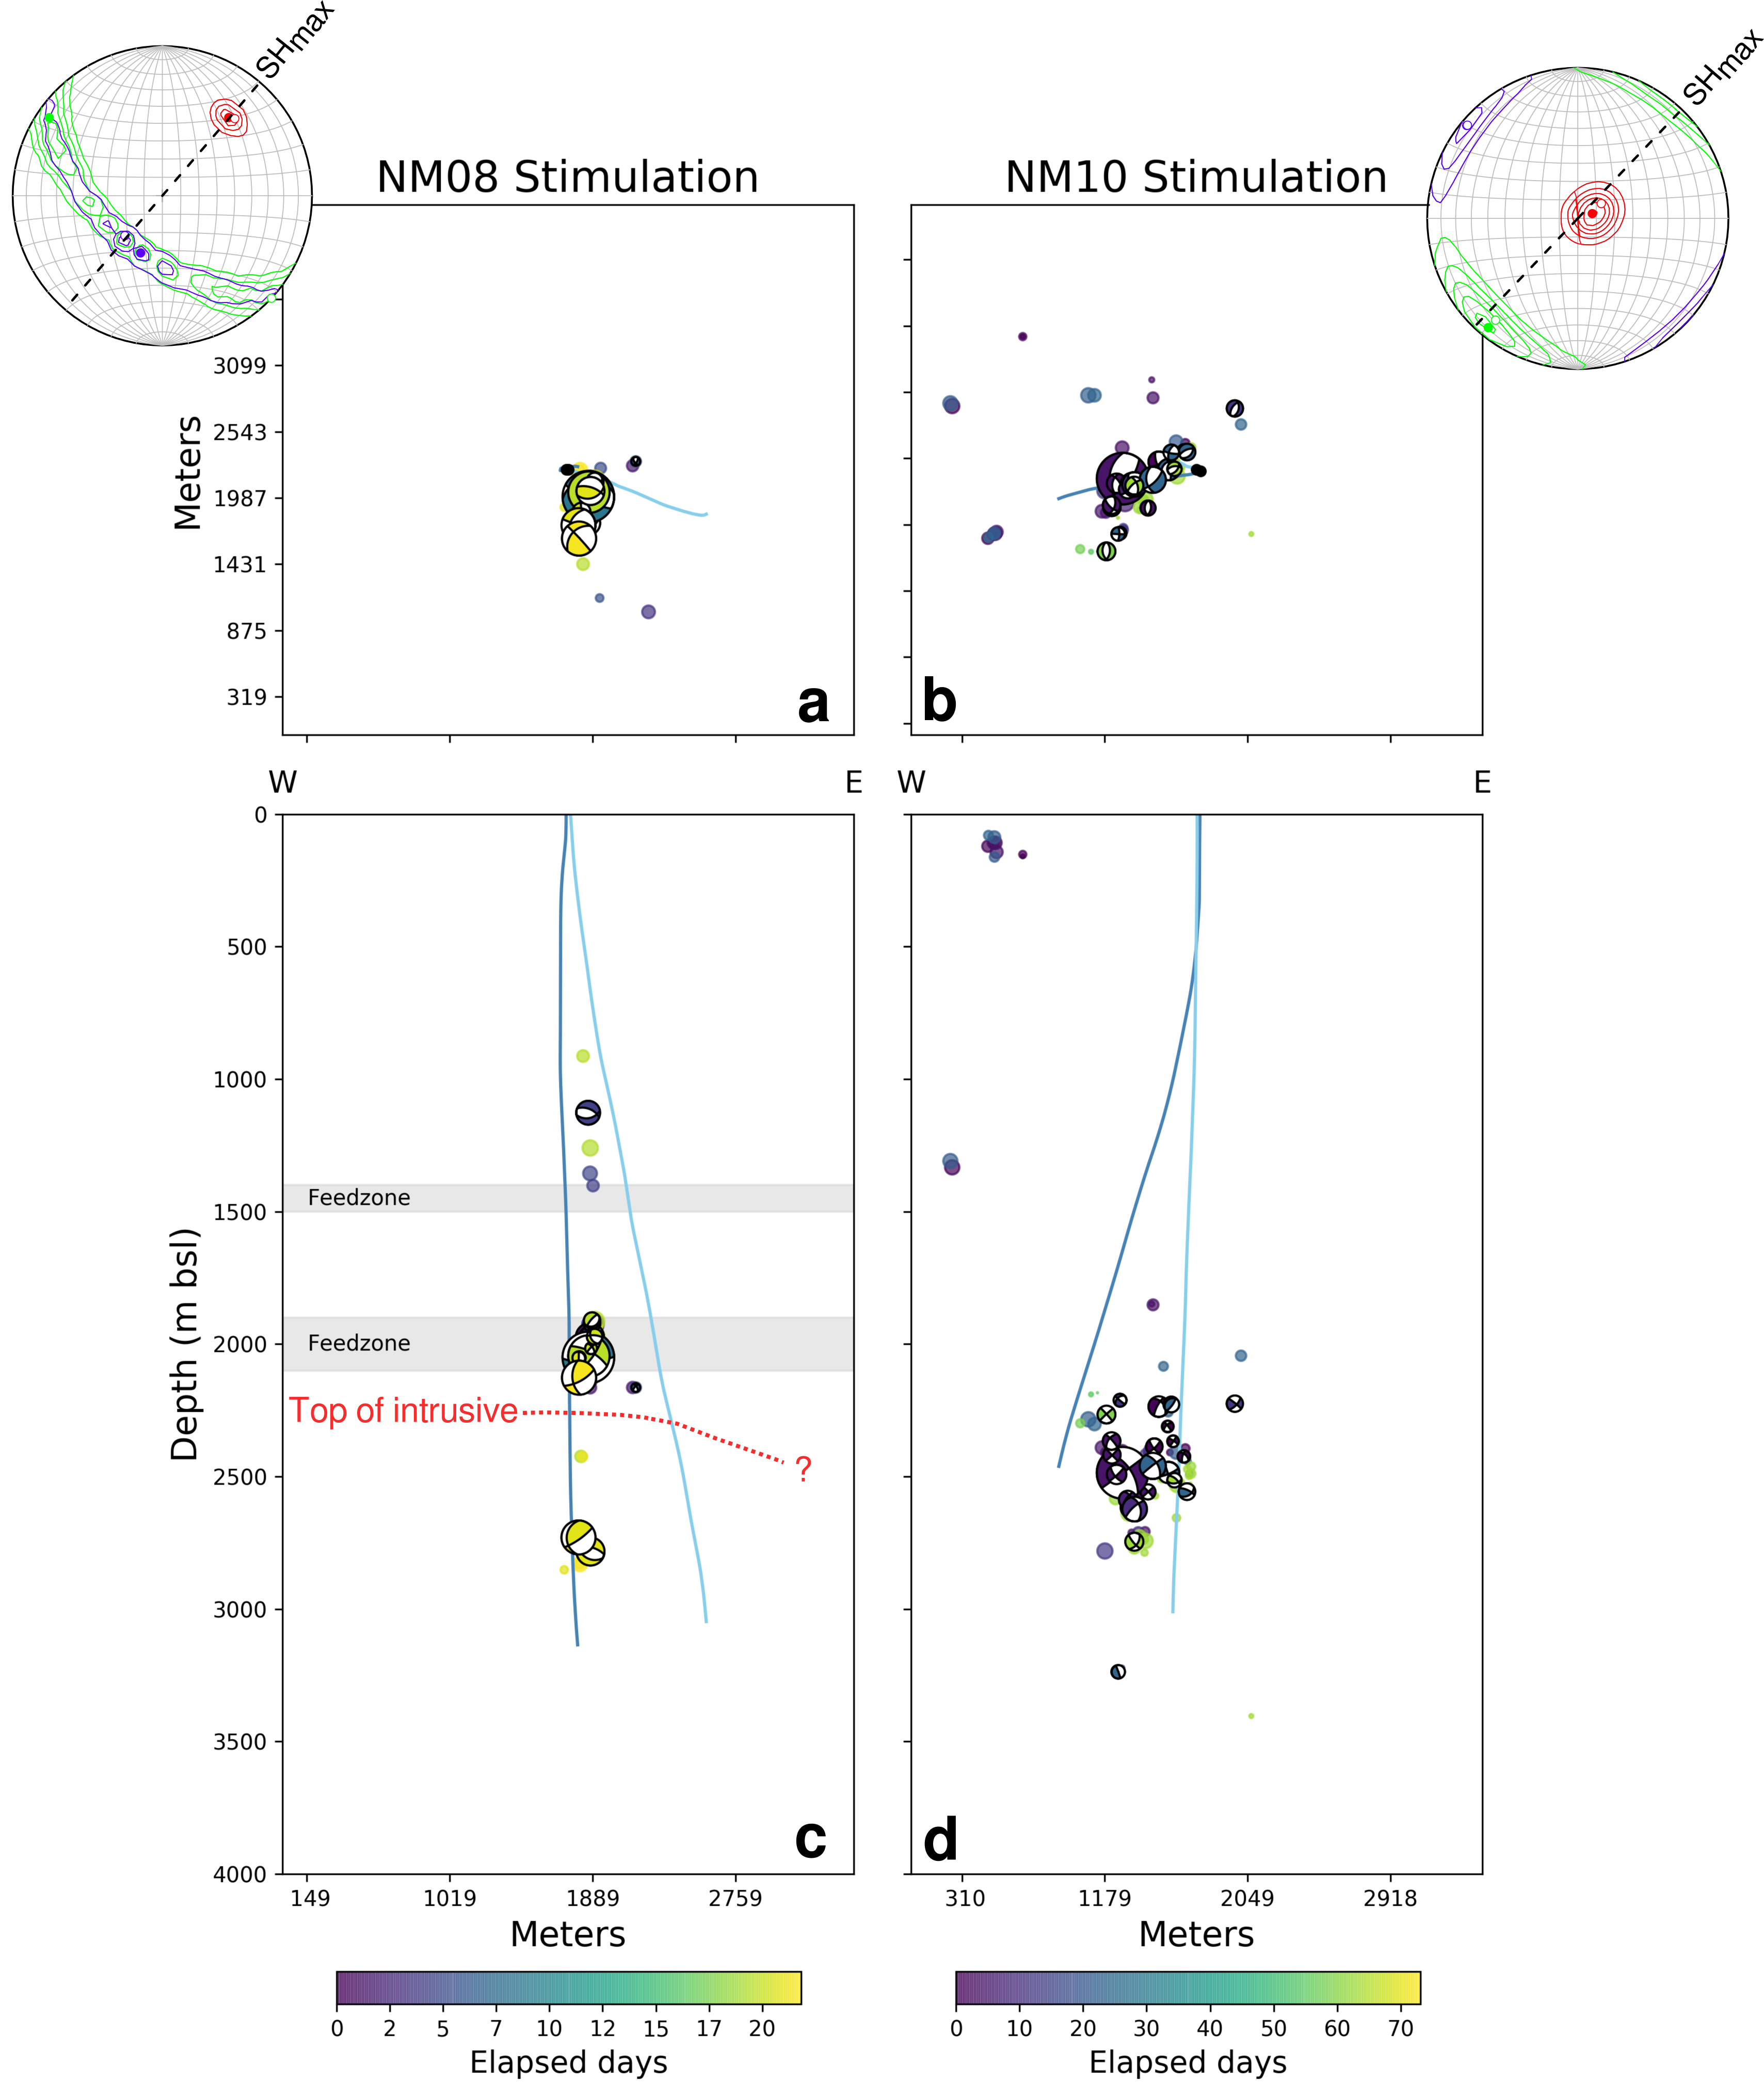
\includegraphics[width=0.84\columnwidth]{Chapter_3_Nga/figures/Nga_stims_map_depth_beachballs_stress_final_labels_10-5_intrusive_colored/Nga_stims_map_depth_beachballs_stress_GC_labels_12-5_intrusive_colored_dpi300_original}
\caption{{P-wave first-motion-derived focal mechanisms for template events which
occurred during various phases of injection testing at Ngatamariki. Dark
blue mechanisms in a and c occurred during stimulation of NM08, in the
northern injection zone. Green mechanisms occurred during NM10 drilling
losses and injection testing (panels b and d; southern zone). The
symbols plotted in cross-sections c and d have been reprojected to
reflect the different viewpoint (from the south). The inset figures in a
and b show stress inversion results (lower hemisphere) from the focal
mechanisms presented in northern and southern Ngatamariki, respectively,
with red contours representing the probability density of the direction
of~\(\sigma_1\), green representing~\(\sigma_2\) and blue
representing~\(\sigma_3\) . The black dashed line indicates the
direction of SHmax. In panel c, the red dashed line indicates the top of
the intrusive sequence in northern Ngatamariki. As the extent of this
unit is only constrained by core from wells NM04 (northeast of panel a),
NM08 and NM09, its shape, volume and orientation are unknown.
{\label{532034}}%
}}
\end{center}
\end{figure}

\subsection{Southern Injection Zone}
\subsubsection{NM10 drilling losses and injection testing}
Well NM06 was drilled and tested in the southern injection zone, many years prior to our study. As a result, drilling and well testing in southern Ngatamariki during this study period was limited to injection well NM10. Injection began once drilling had reached the depth of the deep (andesite) reservoir and drilling-fluid losses occurred (at depths \textgreater2000 m bsl). This was followed by a formal injection\slash{stimulation} test once drilling had been completed. The microseismic response to the drilling losses was larger than the response during the actual injection test (Figures \ref{703798} \& \ref{640752}). At the end of drilling, approximately 57,000 m$^{3}$ of drilling fluid (largely water) had been lost to the formation, a comparable volume to that in the other injection tests analyzed and described above. Data on fluid flow during drilling are sampled less frequently than the flow rate data during injection tests, but daily records of drilling losses correlate well with seismicity in southern Ngatamariki as shown in Figure \ref{703798}a. NM10 drilling reached 1700 m bsl on 6 July 2012 and significant fluid losses were incurred from 13 July ($\sim$2100 m bsl).

Seismicity began as the drilling reached the depth of a major fault zone identified in the NM10 image logs (there are six identified faults between 2100 and 2300 m bsl, within the Rotokawa Andesite \cite{nm10_report}) and continued for the remainder of the drilling (Figure \ref{703798}c). These SE-dipping structures, visible in image logs \citep{nm10_report}, are likely associated with the NE--SW-striking Aratiatia Fault Zone (Figure \ref{795275}, \ref{827409}, \ref{532034}). Seismicity increased in short, 1--2 day-long bursts with the majority of events occurring after fluid losses had exceeded 25 t/h. The lag between the start of fluid losses and the seismicity induced during NM10 drilling is roughly three days, three times shorter than at NM08. This lag may simply be due to the time needed to pressurize the fault zones, which dominate flow from NM10. However, aseismic opening of the fault zones via pore-pressure increase and thermal contraction of the fracture walls, as observed by \citet{Guglielmi_2015}, may also have played a part. We would expect these processes to be accompanied by a corresponding increase in injectivity, but there are no pressure data during the drilling to confirm this. The seismicity occurred \textgreater700 m deeper than the main feedzones in NM10 (Figure \ref{827409}), and closer to injection well NM06, which was shut-in during this period. This may indicate that fluid flowed down-dip along the fault zone to critically stressed points away from the well. The maximum magnitude during drilling at NM10 was 2.1, comparable to the stimulation at NM08 for a similar injected volume. This may indicate that the pressurized zones during NM08 stimulation and NM10 drilling were similar in volume, thereby affecting fractures and faults of similar size. However, as southern Ngatamariki exhibits a lower b-value than in the north when the entire four-year catalog is taken into account, we suggest that much larger structures exist in the south than the north, which were only activated once high-volume injection began in 2013. As at NM08, seismicity ceased after end of drilling implying that the permeability of the fracture zone is considerable.\selectlanguage{english}

\begin{figure}[h!]
\begin{center}
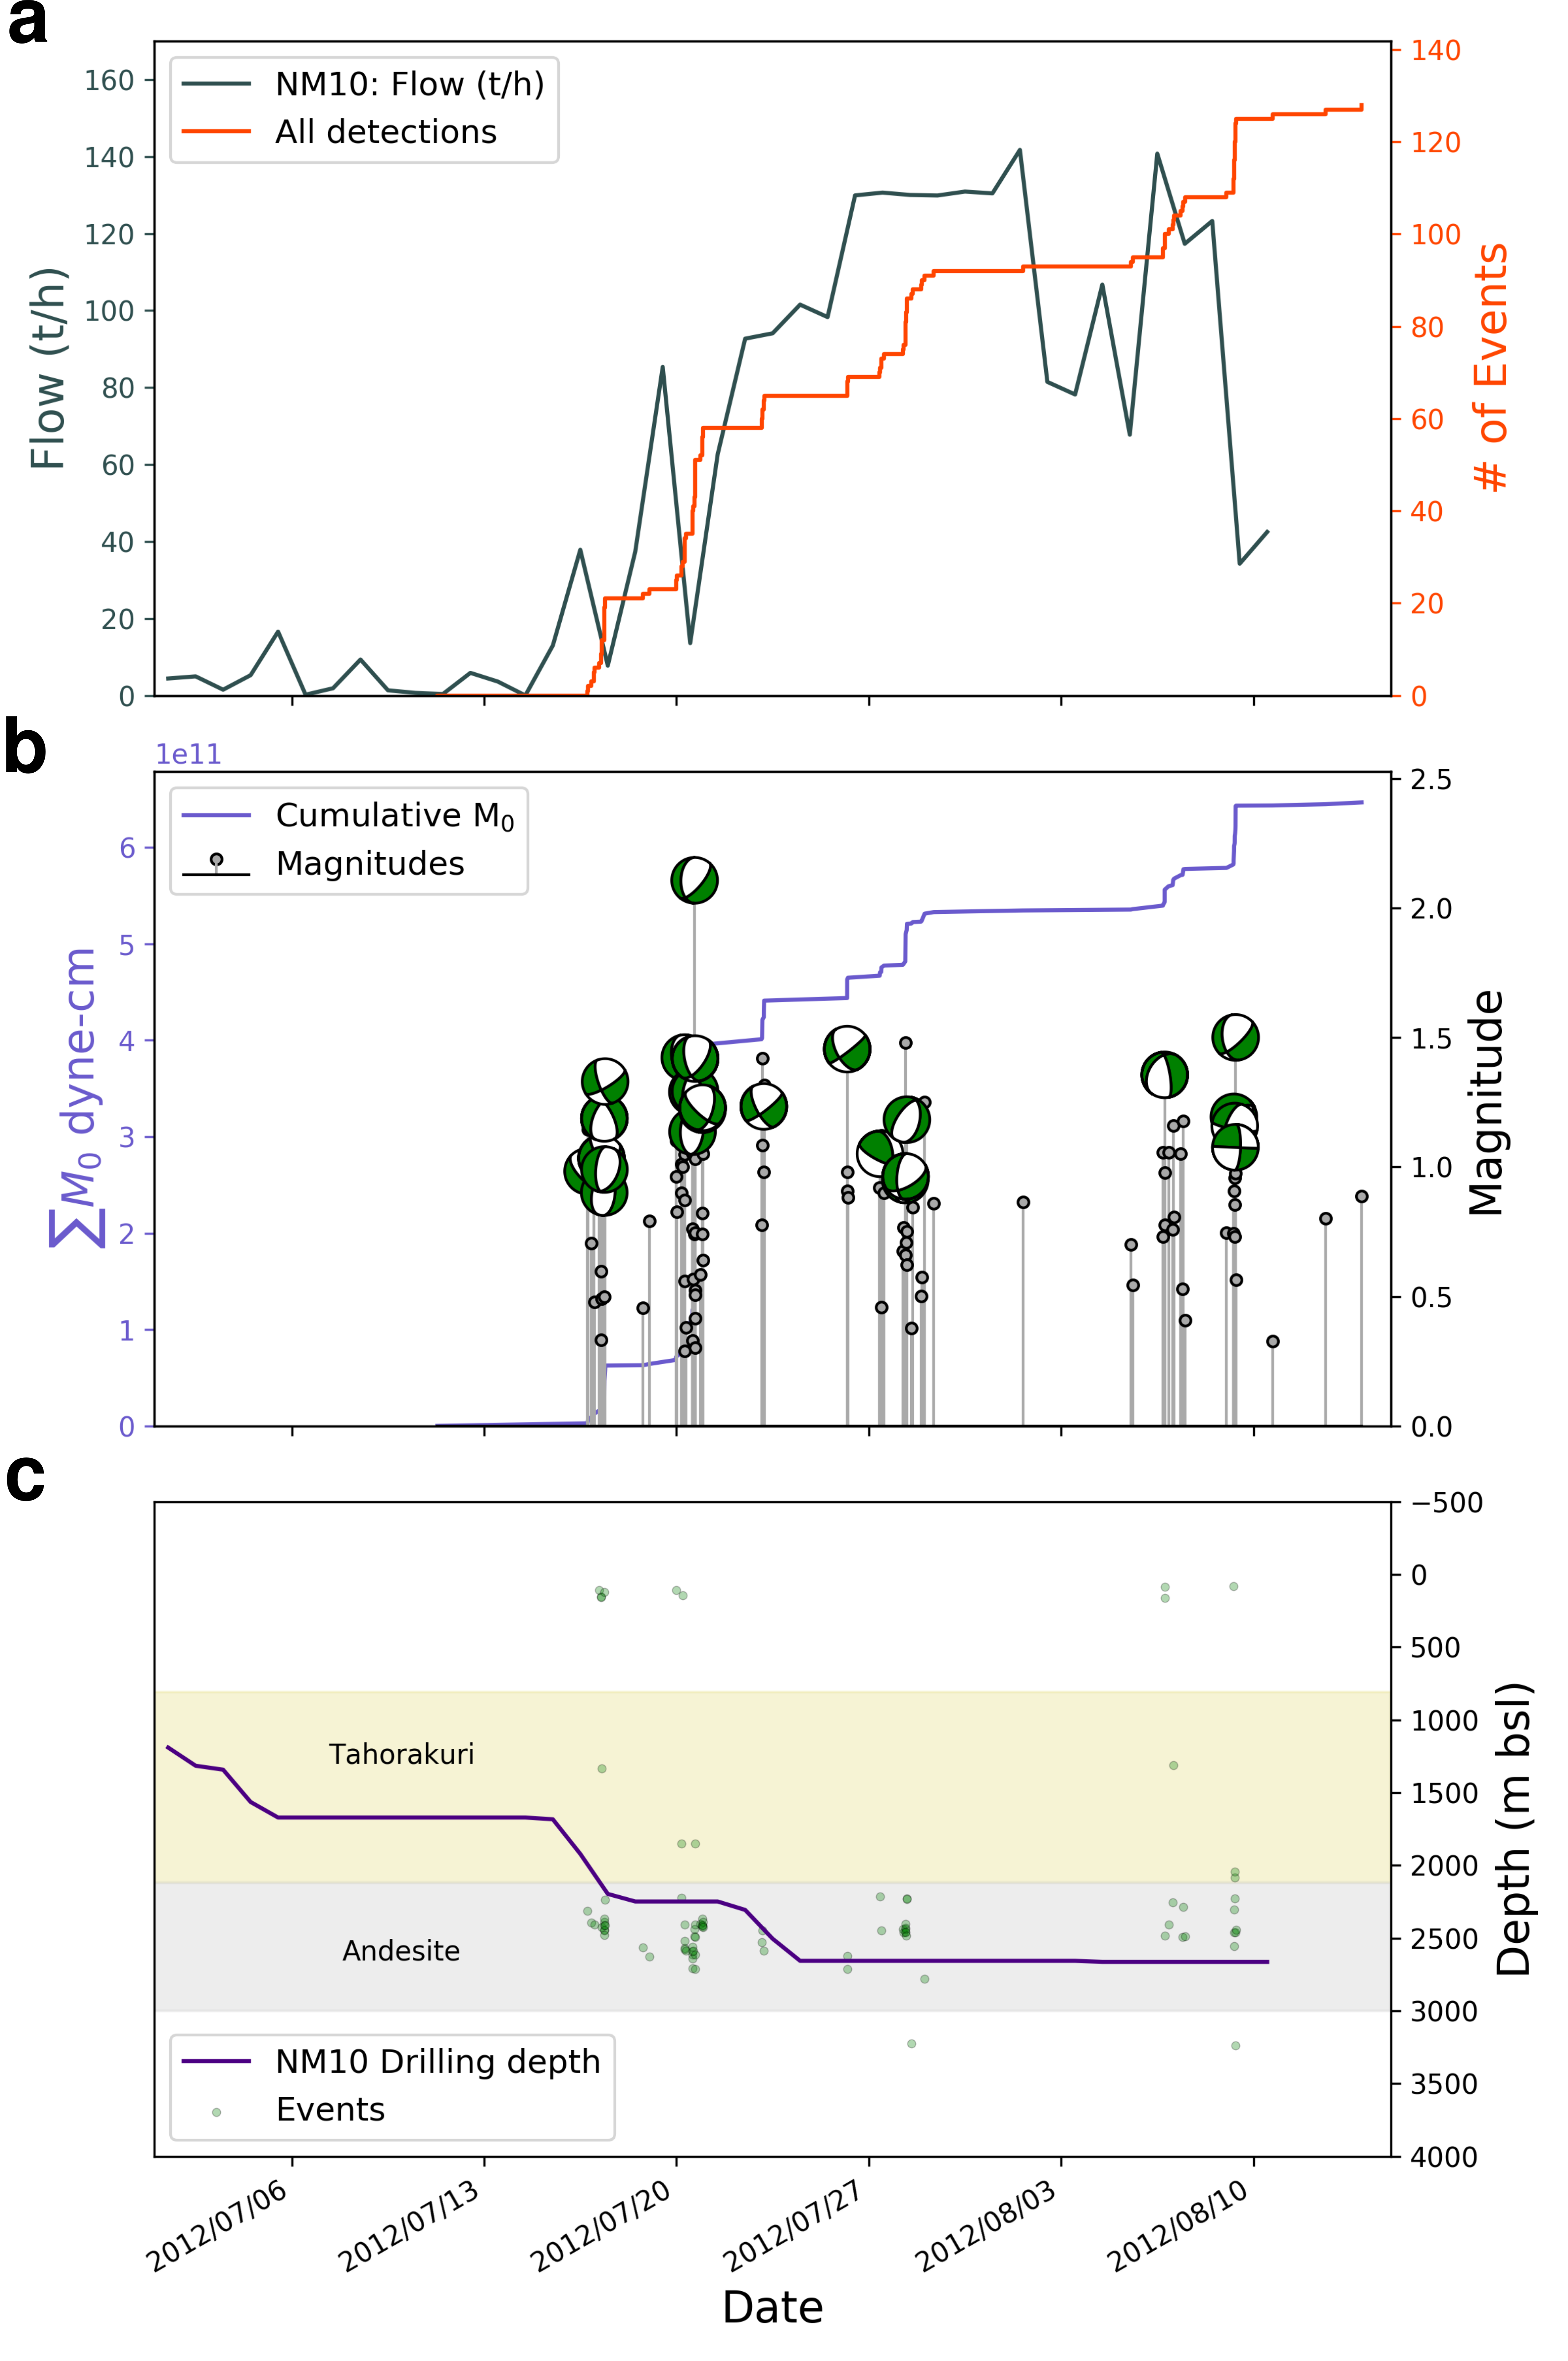
\includegraphics[width=0.84\columnwidth]{Chapter_3_Nga/figures/Multiplet_150_vs_flow_cum_NM10_losses/Full_final_cat_flow_mags_FMs_depth_NM10_Drilling_12-5_GrowClust_no_diff_ABC_original}
\caption{{a) Flow (t/h) during fluid losses and cumulative seismicity vs time, b)
cumulative seismic moment with event local magnitudes and available
focal mechanisms during drilling of NM10 and c) drilling depth with
depth of seismic events. The two main geological units within the
southern reservoir, the Tahorakuri Volcaniclastics and Rotokawa
Andesite, are depicted in c) for context.
{\label{703798}}%
}}
\end{center}
\end{figure}

There were no drilling or injection activities in southern Ngatamariki between the drilling of NM10 and the planned injection test that occurred on 1--23 September, 2012. There was also no detected seismicity during this period. Roughly 73,000 m$^3$ of fluid was injected during the test at flow rates of between 100 and 200 t/h and downhole pressures of 7.5--9.4 MPa (Figure \ref{640752}). As mentioned above, the unintended losses that occurred during drilling are considered the start of injection in southern Ngatamariki. Therefore, during drilling, NM10 may have undergone much of the increase in injectivity that otherwise would have occurred during the later injection test. It is possible that slip during drilling relieved most of the accumulated stress on the most critically stressed portions of the fault zone, making failure on these patches less likely during the injection test. This view is supported by the relative lack of seismicity during most of the test (Figure \ref{640752}). Seismicity, while not absent, occurred for the first two weeks of the test at a rate of roughly one event per day, and injectivity increased only slightly after the first step-rate change in flow from $\sim$100 to 150 t/h. However, the rate of seismicity jumped dramatically (with nearly 40 events on 17 September alone) once injection was increased from $\sim$150 t/h to $\sim$200 t/h. We do not know the corresponding increase in downhole pressure for this step-rate change because the pressure monitoring tubing was repositioned at that time. However, because the flow rate of 200 t/h is significantly higher than was measured during either drilling or testing prior to this time, we can reasonably assume that the downhole pressure would have increased beyond any previously-recorded level at NM10, and therefore would be expected to induce seismicity (again due to the `Kaiser effect' \citep{Holcomb_1993}). The resulting increase in the rate of seismicity occurred within two hours of the increase in flow rate and at event--feedzone distances of up to 800 m (Figure \ref{640752}a and \ref{640752}b). As during FZ2 at NM08, inducing events at such distances so rapidly requires that pressure change be concentrated along a small number of highly-permeable fracture zones, which is what we expect in NM10 on the basis of image logs. Once flow rate had subsided to below 200 t/h, seismicity ceased, suggesting rapid progression of the back-front to the seismically active zone as was observed at NM08. The maximum magnitude during the injection testing of NM10 was 1.4, lower than during NM10 drilling, possibly as a result of the stress acting on the fracture zone having been relived during drilling fluid losses.\selectlanguage{english}

\begin{figure}[h!]
\begin{center}
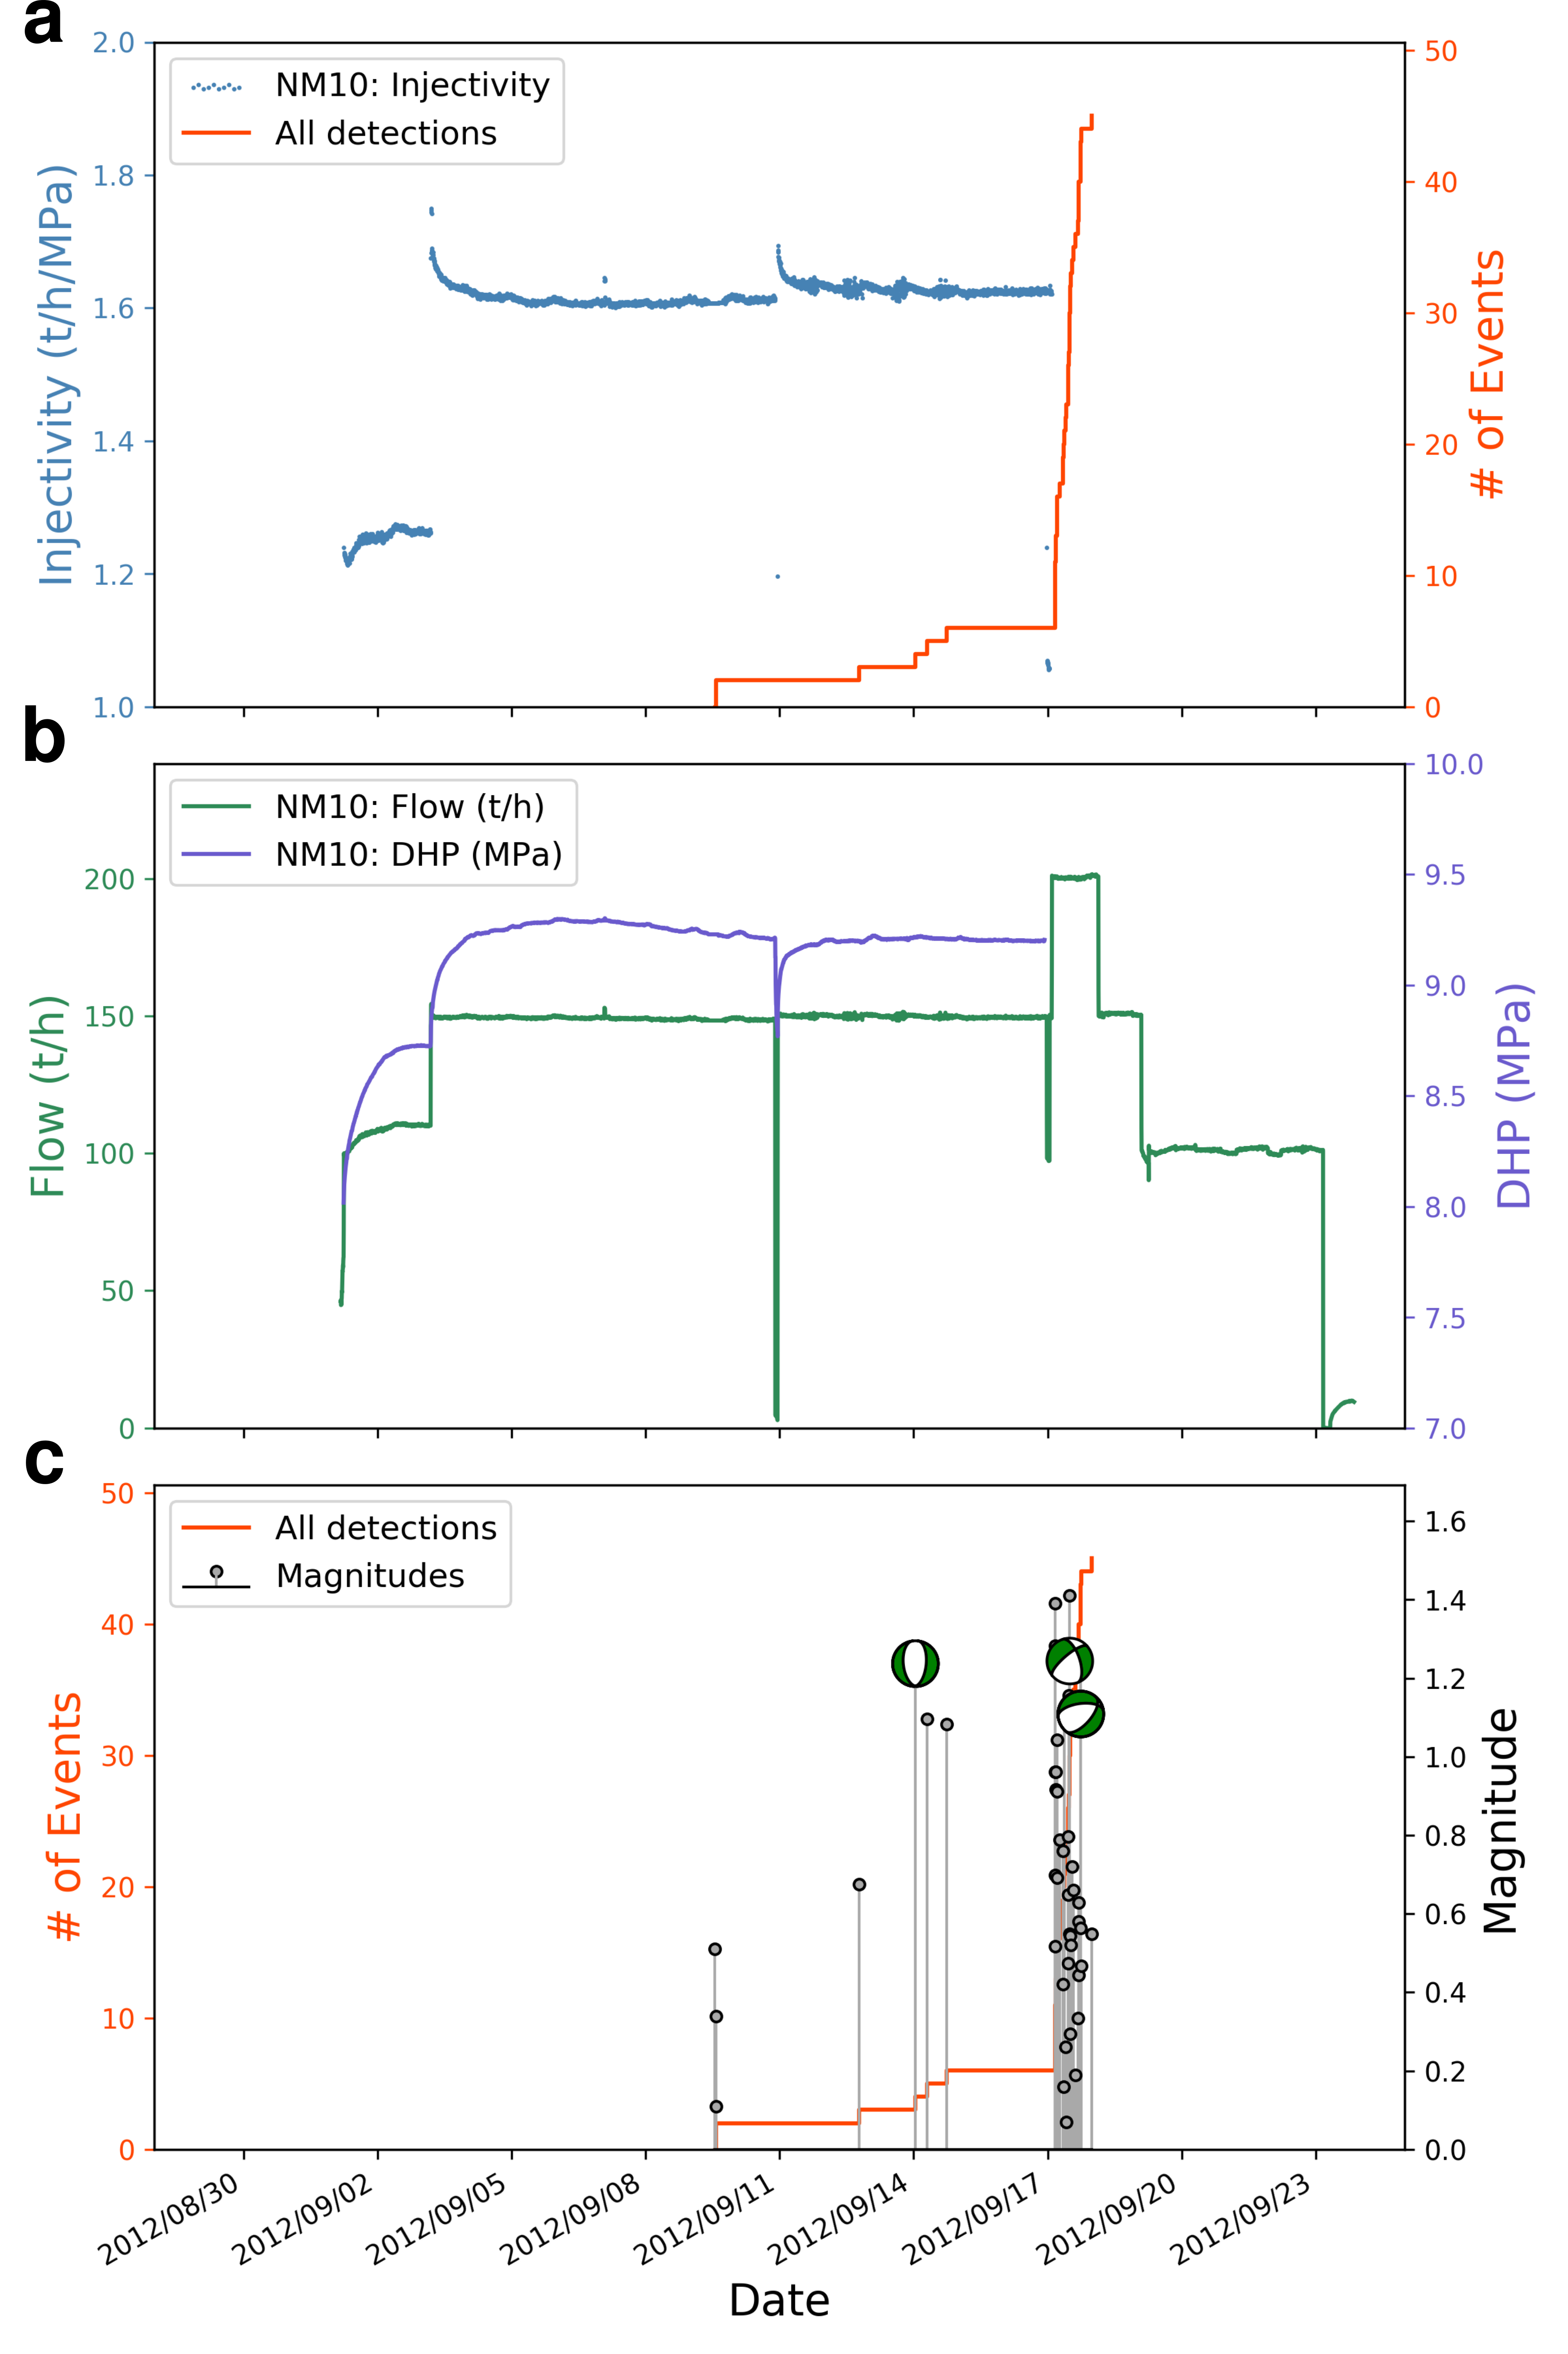
\includegraphics[width=0.84\columnwidth]{Chapter_3_Nga/figures/Multiplet_150_vs_flow_cum_NM10_stim/Full_final_cat_flow_mags_FMs_depth_NM10_Stimulation_12-5_GrowClust_labels_no_diff_ABC_original.png}
\caption{{a) NM10 injection test II vs. cumulative seismicity in southern
Ngatamariki, b) Flow rate and downhole pressure. DHP ends on 17 Sept as
the measurement tubing was traversed to a greater depth (from 1228 m to
2050 m). c) Cumulative seismicity in red with the magnitude and
available focal mechanism solutions as stems.
{\label{640752}}%
}}
\end{center}
\end{figure}

\subsection{Focal mechanisms and stress}
Figure \ref{532034} shows the focal mechanisms calculated for microearthquakes that occurred during the three well injection tests described above, and the corresponding stress inversion results for northern and southern Ngatamariki prior to plant startup. The events that occurred during drilling and injection testing of NM10 (Figure \ref{532034}b and d) delineate a structure associated with the Aratiatia Fault Zone, as mentioned above. The majority of the 28 focal mechanisms we calculated for southern Ngatamariki during this time period show predominantly normal faulting, with most fault planes striking N--S or NE--SW. This result agrees well with what is known about the extensional regional stress regime and the local faults in the central TVZ, which are typically oriented NE--SW \citep{Massiot_2015}. Acoustic- and resistivity-based image logs for NM10 confirm this preferred NE--SW fracture orientation at reservoir depths with predominantly SE dips \citep{nm10_report}. As mentioned in Sections \ref{Plant_ops} and \ref{location_results}, rapid injection returns during a tracer test conducted in January 2014 also indicate that a highly permeable flow pathway connects NM10 to production well NM05 \citep{buscarlet_2015}. The locations of the events induced during NM10 drilling and injection testing are likely related to fluid flow along this structure.

Stress inversion results for southern Ngatamariki (inset, Figure \ref{532034}b) show $\sigma_1$ to be subvertical and the direction of maximum horizontal compressive stress ($S_{HMAX}$) to be NE--SW, consistent with previous findings for the central TVZ \citep{Townend_2012} as well as measurements of borehole breakout in NM10 which indicate an $S_{HMAX}$ azimuth of 210\textdegree \citep{nm10_report}. This result is also consistent with breakout measurements from the Rotokawa geothermal field, 5 km to the south \citep{McNamara_2015}.

The 58 blue mechanisms in Figure \ref{532034}a and c correspond to events that occurred during the stimulation of NM08 and exhibit a greater variety of faulting kinematics than in the south. Many of these mechanisms show primarily reverse or oblique strike-slip movement with at least one nodal plane striking NW--SE, which agrees with the orientation of the plane defined by the hypocenters of the events (strike 192\textdegree, dip $\sim$66\textdegree). The remaining mechanisms show normal faulting with a variety of strikes. The occurrence of compressional faulting is rare within the central TVZ and may be related to stress field rotation during the emplacement of the intrusive body and mafic dikes.

Stress inversion results for northern Ngatamariki differ from those in the south (insets in Figure \ref{532034}a and b). While the direction of $S_{HMAX}$ is unchanged throughout the reservoir (NE--SW), $\sigma_1$ is dipping NE at approximately 30\textdegree{} in the north and $\sigma_2$ and $\sigma_3$ define a girdle. It is possible that the stress state in this section of the reservoir was already rotated into an orientation suitable for reverse faulting by the emplacement of the tonalite intrusive body and dikes. \citet{massiot_2012} showed that the in-situ horizontal stress field rotates counter-clockwise by 28\textdegree{} near the contact between the Tahorakuri and the intrusive body (below the main permeable zone and dikes, relative to the stress field above), which may indicate an intrusive-related effect on the stress state.

What is not known is the effect of injection-related pressure buildup and thermoelastic stresses on the stress in the reservoir (Figure \ref{111394}). We have no DHP measurements during stimulation of NM08. However, wellhead pressure reached 2.6 MPa during the near-field period of stimulation (NF, Figure \ref{645772}). Figure \ref{111394}a shows the destabilizing effect of pore pressure increase on the reservoir stress state, with the increase in P$_f$ exaggerated for visibility. We infer that the fracture zone defined by the seismicity during NM08 stimulation is nearly-critically-stressed within the reservoir stress regime and would require only small increases in pore pressure to induce slip (blue and red circles, Figure \ref{111394}a).

Circumferential stresses reached roughly -54 MPa at the wellbore (at 2000 m bsl), but it is difficult to determine how far such thermoelastic effects would propagate from the well as the propagation of the thermal front is dependent upon the flow pathways and flow rate through the reservoir. During a stimulation operation at the naturally-fractured Geysers geothermal field, \citet{Jeanne_2015tensor} modeled a similar thermal front propagating \textgreater100 m in the span of two months. For a reservoir where fluid flow is fracture dominated, the corresponding cooling effect depends on the predominant direction of flow relative to the principle stress axes, as illustrated in Figure \ref{111394}b \citep{Jeanne_2015tensor}. This is because the rock matrix is cooled conductively only within \textless1 m along the normal to a fracture plane, whereas it is cooled for many tens of meters along the strike of a fracture, leading to an anisotropic volume of thermal cooling \citep{De_Simone_2013,Jeanne_2015tensor}. Initial, gravity-driven (downward) flow of cool fluid at NM08 would preferentially decrease $\sigma_{1}$ and stabilize the near-well fracture network (yellow Mohr circle, Figure \ref{111394}b). This may have contributed to the lack of seismicity during the NF and BT periods of NM08 stimulation (Figures \ref{645772} and \ref{740510}). As fluid begins to spread laterally from the well, the cooling effect preferentially lowers the horizontal stress that is best aligned with the direction of flow. At Ngatamariki, fluid flow parallel to $\sigma_{3}$ (NW--SE) would act to destabilize the fracture network (pink Mohr circle, Figure \ref{111394}b), including the structure along which seismicity occurred, which is represented as a colored circle for the various stress fields illustrated in Figure \ref{111394}.

As the Ngatamariki reservoir is structurally similar to that of the Geysers, in that they are both naturally-fractured, high-temperature fields, it is possible that a thermoelastic front could have reached the location of seismicity during stimulation of NM08 and therefore influenced the stress state in the fracture zone. Also at the Geysers, \citet{Mart_nez_Garz_n_2013} observed temporal changes in focal mechanism-derived stress tensors related to various fluid injection operations (including the injection operation modeled by \citet{Jeanne_2015tensor}), although this contrasts with the findings of \citet{Boyle_2014} who found that operations at the Geysers had little effect on the reservoir stress state. We cannot rule out the possibility that the deviation of the stress field from the regional trend in northern Ngatamariki is injection-related, although we think it unlikely. As discussed above, it is also possible that the stress state was already rotated in the northern injection zone prior to injection.\selectlanguage{english}

\begin{figure}[h!]
\begin{center}
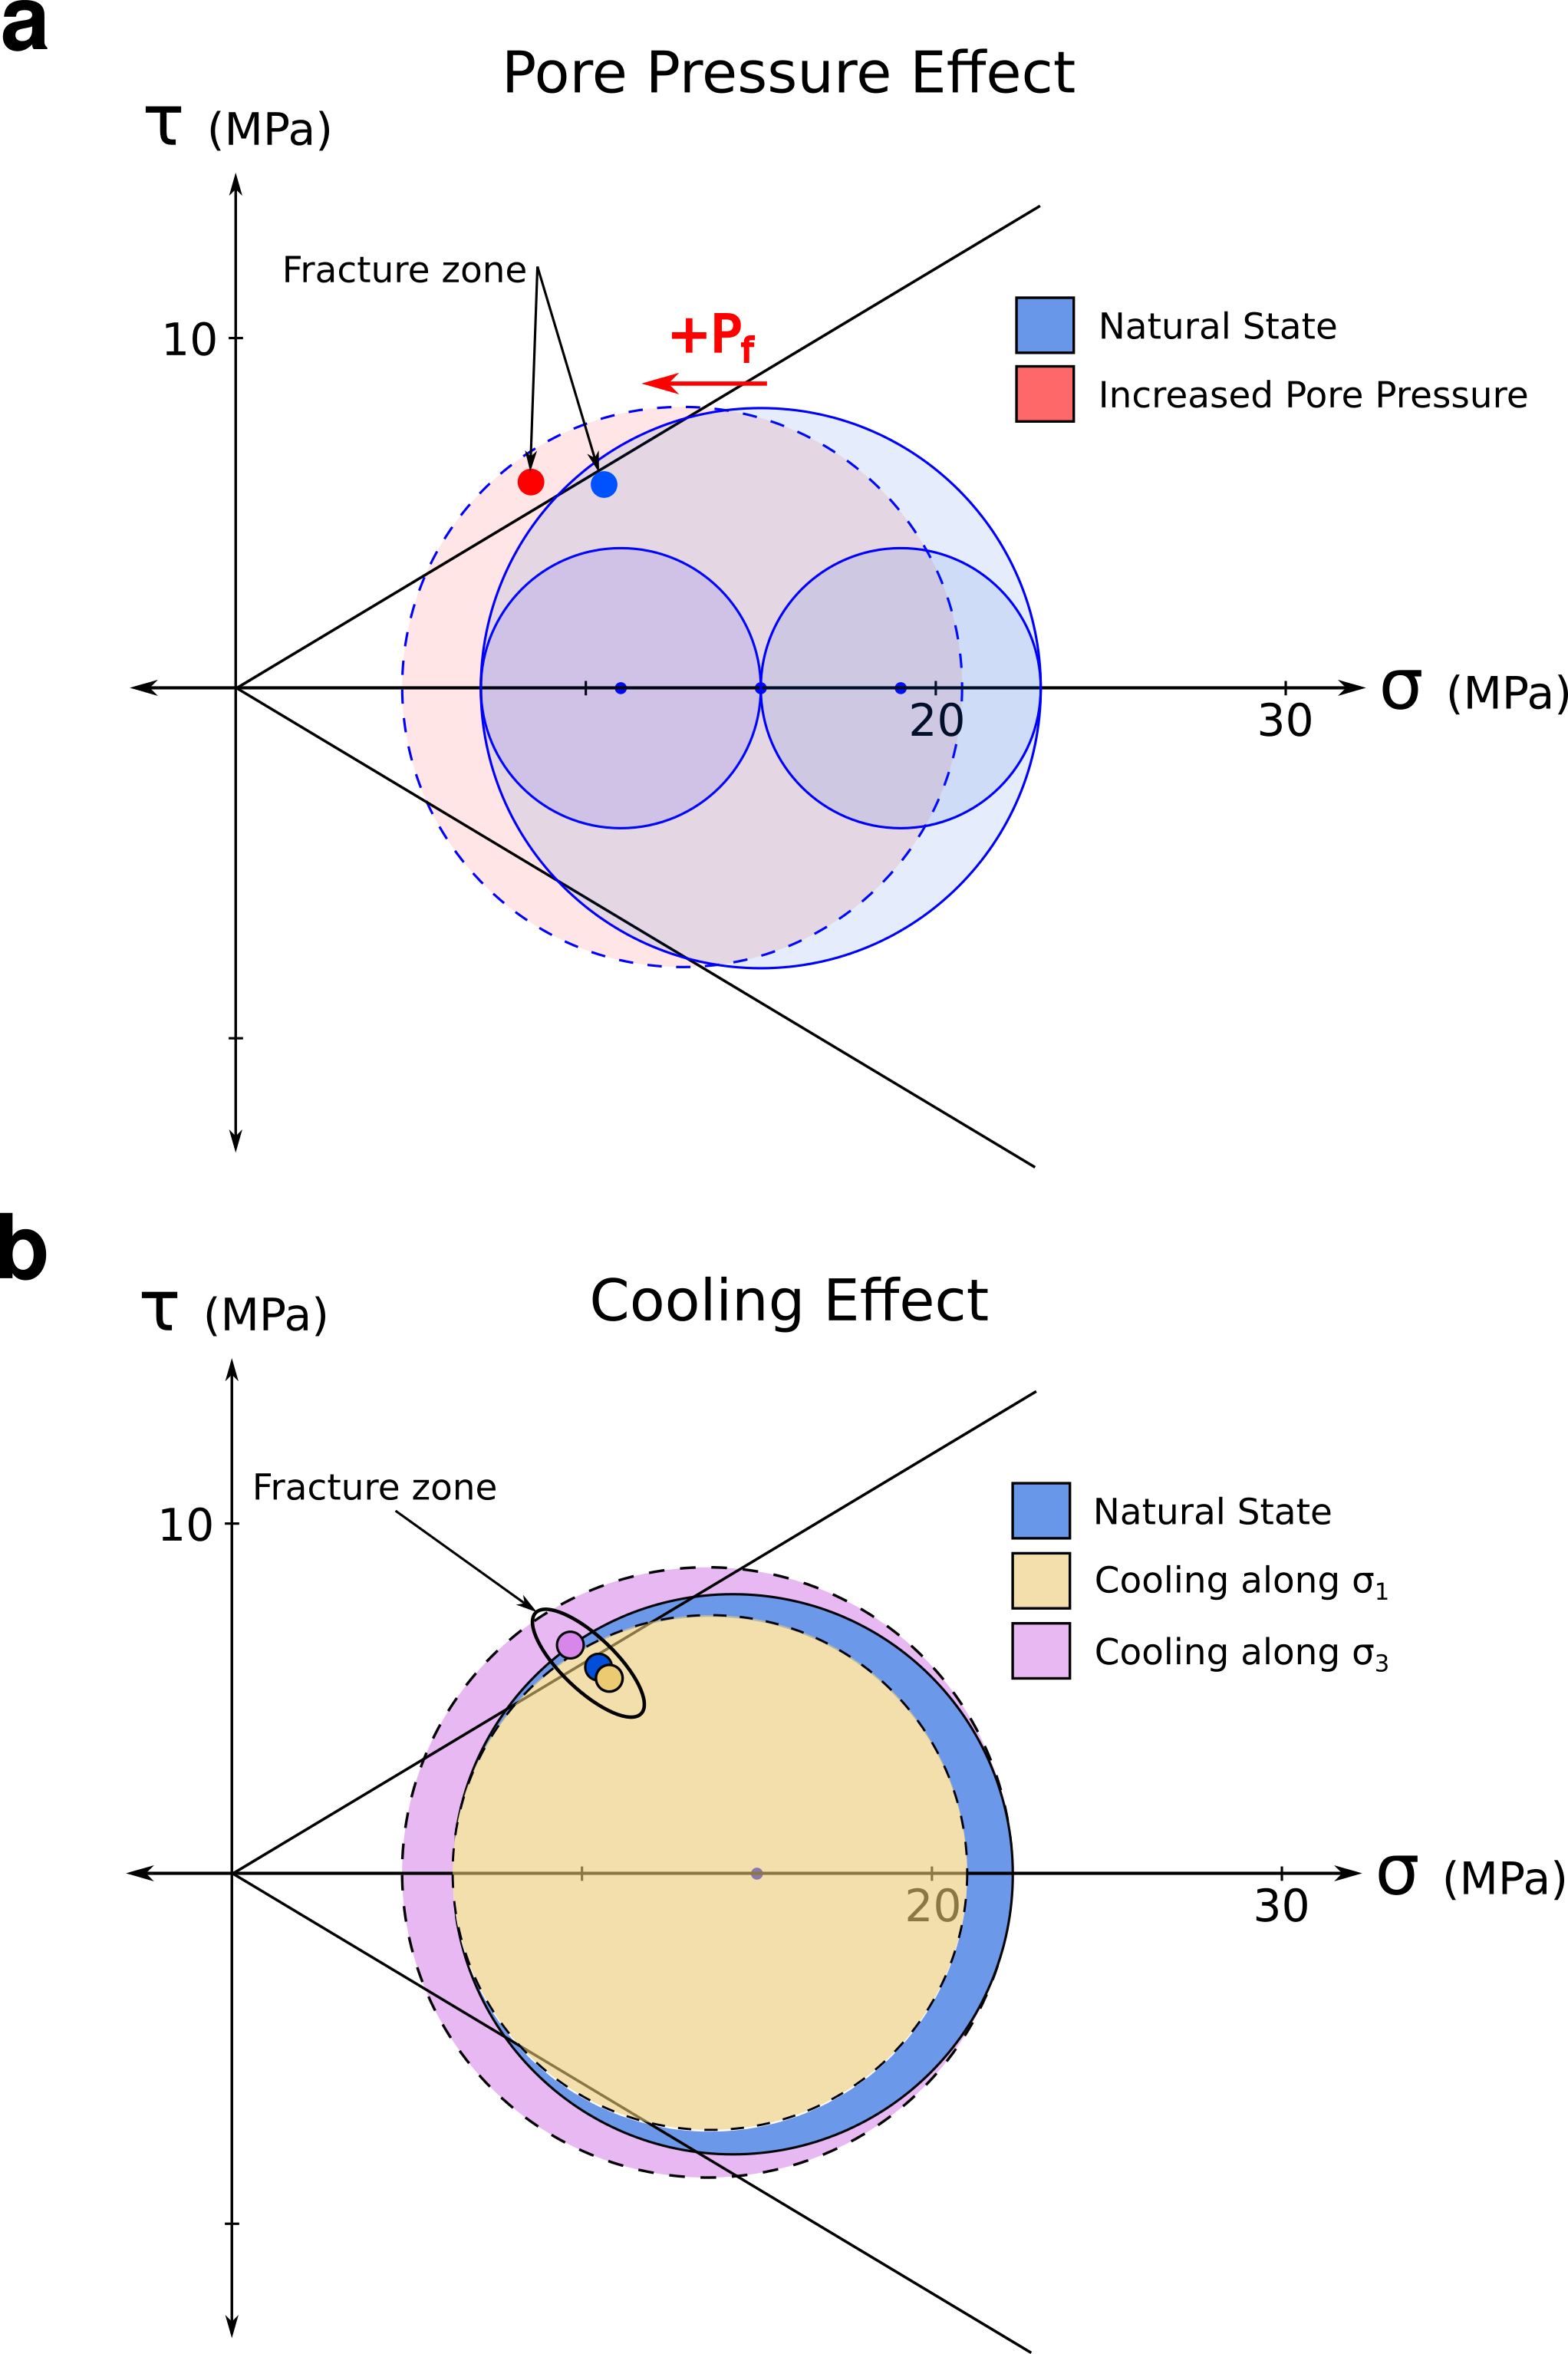
\includegraphics[width=0.70\columnwidth]{Chapter_3_Nga/figures/Nga_2000mbsl_NM08_fz_schematic/Nga_2000mbsl_NM08_fz_schematic_original.png}
\caption{{Schematic Mohr circles calculated for a depth of 2000 m bsl illustrating
the effect of a) pore pressure increase and b) thermal cooling of the
fracture zone near well NM08 (strike: 191\textsuperscript{o}, dip:
66\textsuperscript{o}). The natural state magnitude
for~\(\sigma_{1}\) was determined by integrating density over depth
using density values from well cuttings and core taken from NM08
($\sim$45 MPa at 2000 ms). The magnitude
of~\(\sigma_{3}\) was extrapolated from leak-off tests conducted in
Rotokawa ($\sim$29 MPa)~\protect\citep{davidson_2012}. Reservoir
pressure is approximately 22 MPa at 2000 m bsl. The failure envelopes
represent cohesionless, preexisiting fractures with a coefficient of
friction of 0.6. Circles in the figure represent the position of the
plane defined by the hypocenters of seismicity during NM08 stimulation
within each stress field. Plots are adapted from the output
of~\href{http://www.geo.cornell.edu/geology/faculty/RWA/programs/mohrplotter.html}{MohrPlotter}~\protect\citep{Allmendinger}.
{\label{111394}}%
}}
\end{center}
\end{figure}

\section{Conclusions}
Ngatamariki constitutes an important case study of isolated injection into a little-modified reservoir. In this paper we present a nearly four-year catalog of microearthquakes at the Ngatamariki geothermal field spanning periods of initial field development, well drilling and plant startup. Individual tests at each well were isolated from one another in both time and space, which has allowed us to observe the response of microseismicity to injection at individual wells. Seismicity occurs in two spatial clusters centered on the northern and southern injection zones. In the north, stimulation of well NM08 induced more than 120 events in one month, while injection testing of nearby well NM09 generated only 11 events in nearly three months. In southern Ngatamariki, drilling and injection testing of NM10 generated nearly 200 events over an interval of roughly three months. The difference between the frequency-magnitude distributions of the northern and southern clusters provides a clear example of b-value dependence on the characteristics of the local fracture network. In the north, the fractures that are hydraulically connected to wells NM08 and NM09 are smaller than those in the south, where fluid is injected into a large, active fault zone. As a result, larger events are able to nucleate in the southern injection zone (b$=$1.20) than in the north (b$=$1.84), resulting in a lower b-value.

Focal mechanisms calculated for events that occurred during these injections show different faulting regimes in the northern and southern halves of Ngatamariki. During the stimulation of NM08, in the northern part of the field, focal mechanisms exhibited a wide range of faulting kinematics, most with at least one nodal plane consistent with the NNE--SSW trend in hypocenter locations and a stress state with $\sigma_{1}$ dipping 30\textdegree. In contrast, NE--SW-striking normal faulting mechanisms make up the bulk of events occurring in the south. We interpret this contrast to be related to the presence of the tonalite intrusive body encountered at the bottom of the wells in northern Ngatamariki, which likely modified the local stress field in such a way that reverse and strike-slip faulting could occur in close proximity. However, as has been modeled and inferred for the Geysers geothermal field, another high-temperature, naturally-fractured reservoir \citep{Mart_nez_Garz_n_2014,Jeanne_2015tensor}, injection-induced stress tensor changes are plausible at Ngatamariki.

Fluid injection-induced slip on nearby, suitably oriented fractures is commonly assumed to be the main mechanism responsible for well stimulation. In the Ngatamariki case, however, induced seismicity occurs independently of near-well permeability gain, suggesting that seismic slip and permeability gained through self-propping play a subsidiary role in well stimulation. During the cold-water stimulation test at NM08, injectivity increased rapidly from the start of injection with no apparent sensitivity to the onset of seismicity ten days later. During injection at NM09, the well was also stimulated but was accompanied by only 11 detected seismic events despite two separate injections totaling \textgreater100,000 m$^3$ of fluid. In the south, interpretation of the cold-water stimulation of well NM10 was complicated by fluid losses during drilling, which induced nearly 140 events but for which no injectivity data exist.

This apparent decoupling of induced seismicity and near-well permeability suggests that slow, aseismic processes dominate well stimulation at Ngatamariki, specifically, but also at other high-temperature, high-permeability geothermal reservoirs where thermo-elastic stresses may lead to fracture opening but not necessarily to seismic slip. Other recent studies have raised the possibility that permeability and seismicity need not be related for cases of induced seismicity \citep[e.g.][]{Guglielmi_2015, Riffault_2018} and the dataset we present here contributes to the documentation and understanding of this discrepancy.

The degree of decoupling may be a product of the combined high-permeability and high-temperature of the Ngatamariki reservoir. Lower-temperature resources will not exhibit similar degrees of thermal stimulation and lower-permeability reservoirs are subject to higher pore-pressure perturbations, thus increasing the likelihood of inducing seismicity. However, if permeability enhancement and seismicity are decoupled, as we have shown for Ngatamariki, it may be possible to design injection operations in similar settings elsewhere in order to achieve the desired permeability gain while limiting the number and magnitude of induced seismic events.

\section{Acknowledgments}
We thank the Rotokawa Joint Venture (Tauhara North No. 2 Trust \& Mercury NZ Limited) for the funding to conduct this research and for allowing us access to the data and permission to publish our findings. We also wish to acknowledge the contribution of high-performance computing facilities to the results of this research. New Zealand's national facilities are provided by the NZ eScience Infrastructure (NeSI) and funded jointly by NeSI's collaborator institutions and the Ministry of Business, Innovation \& Employment's Research Infrastructure program (https://www.nesi.org.nz). The analysis reported here made use of the ObsPy seismic processing toolbox \citep{obspy_doi}, and the matched-filter detection was conducted using the EQcorrscan package \citep{Chamberlain_2017, eqcorrscan_doi} which can be freely downloaded and installed via \href{https://pypi.python.org/pypi/EQcorrscan}{PyPI} or \href{https://anaconda.org/conda-forge/eqcorrscan}{Anaconda} on all major platforms. The documentation is hosted at \href{http://eqcorrscan.readthedocs.io/en/latest/}{ReadTheDocs}.

The final version of the Ngatamariki earthquake catalog can be found at DOI \href{10.17605/OSF.IO/C2M6U}{10.17605/OSF.IO/C2M6U} along with access to the github repository of all scripts used in this work.

% 	\cleardoublepage
% 	\chapter[Seismic response to evolving injection at Rotokawa geothermal field, New Zealand]{Seismic response to evolving injection \\at Rotokawa geothermal field, \\New Zealand}

\section*{Abstract}
While simple spatial locations of seismicity can provide valuable
insights about reservoir structure and fluid movement,
frequency-magnitude distributions, often of secondary interest to
operators, may contain unique information about the distribution of
pressure. In this work, we present a four-year catalog of seismicity for
the Rotokawa geothermal field in the central Taup\={o} Volcanic Zone, New
Zealand starting two years after the commissioning of the 140 MW Nga Awa
Purua power station. Using waveform-correlation-based signal detection
we double the size of the previous earthquake catalog and update the
location and orientation of two important reservoir faults, while
identifying a new structure. We find the rate of seismicity
to be insensitive to major changes in injection strategy during the
study~period, including the \gls{injectivity} decline and shift of injection
away from the dominant injector, RK24. We also map the spatial
distribution of the earthquake frequency-magnitude distribution,
or~\emph{b}-value. Although complex, the spatial variation of~\emph{b}
can potentially be used to monitor the relative distribution of pressure
in the reservoir, where areas of high~\emph{b} correspond to areas of
high pore-fluid pressure and a broad distribution of activated fractures. While
not routinely conducted, we believe our results show promise for using
earthquake $b$-value as an additional tool for reservoir monitoring
and management.

\section{Introduction}
Geothermal operators routinely monitor rates and locations of microseismic activity at developed reservoirs. Typically, the location of seismicity is assumed to correlate with regions where pore-fluid pressure has been artificially elevated by fluid injection \citep[e.g.][]{Sherburn_2015,Garcia_2016}. In turn, these areas are assumed to correspond to major flow pathways in the reservoir, which are of paramount importance in understanding reservoir dynamics and planning injection\slash{extraction} well targets. In addition, reservoir structures can be accurately imaged from high-precision earthquake hypocentral locations, as can the extent of the permeable reservoir \citep{Sewell_2015WGC}.

However, much of the information contained in even a basic earthquake catalog can go unused by reservoir managers. Specifically, while earthquake magnitudes are nearly always calculated during automated processing of seismic data, this information goes relatively unnoticed. In a limited number of cases, magnitude information has been used to infer reservoir properties such as pore-fluid pressure and the extent of fracturing. For example, \citet{Bachmann_2012} modeled $b$-value and pore-fluid pressure for the case of the Basel enhanced geothermal injection well, showing that $b$ is expected to decrease exponentially with distance from a given injection point, but that $b$ actually increased between the wellbore and 200 m for reasons that weren't immediately clear. Given the inclusion of event magnitude data in nearly every earthquake catalog, more attention should be paid to patterns in frequency-magnitude distributions as a tool for reservoir management.

In this paper we focus on the Rotokawa geothermal field in the central Taup\={o} Volcanic Zone of New Zealand. The field was initially developed in 1997 but has undergone large-scale development since that time, most significantly the commissioning of the 140 \acrfull{MWe} \acrfull{NAP} plant in 2010 \citep{McNamara_2016}. The seismic dataset analyzed here (2012--2015) corresponds to a period of stabilization, during which the reservoir was equilibrating to the increased extraction required by the installation of NAP. We use a matched-filter earthquake detection technique to substantially increase the number of events in our catalog relative to standard, automatic detection. We then calculate magnitudes for the newly detected events, again using a waveform correlation-based technique before precisely relocating each event. 

Over its two decades of development, the Rotokawa reservoir has been relatively well studied. The current understanding of the reservoir is based on research from a number of workers who have identified at least four compartments, which are likely bounded by a number of faults acting as barriers to inter-compartment flow \citep{Sewell_2015,Addison_2017stanford,wallis2013}. Previous studies of microseismicity at Rotokawa have been used to constrain the location of one of these structures, the Central Field Fault, but due to its confinement to the injection field compartment, seismicity has been unable to reveal further structure within the reservoir \citep{Sherburn_2015,Sewell_2015WGC}.

In the following analyses, we compare our catalog to the catalogs of previous studies of microseismicity at Rotokawa \citep{Sewell_2015WGC,Sherburn_2015} and relate the rate and location of seismicity to changes in injection strategy at Rotokawa. We also map the frequency-magnitude distribution ($b$-value) within the field, something which has not been done at Rotokawa before. While the observed patterns in $b$-value are quite complex, when combined with high-precision locations, they show potential for mapping of pore-pressure and/or fracturing extent at a reservoir scale.\selectlanguage{english}

\begin{figure}[p]
\begin{center}
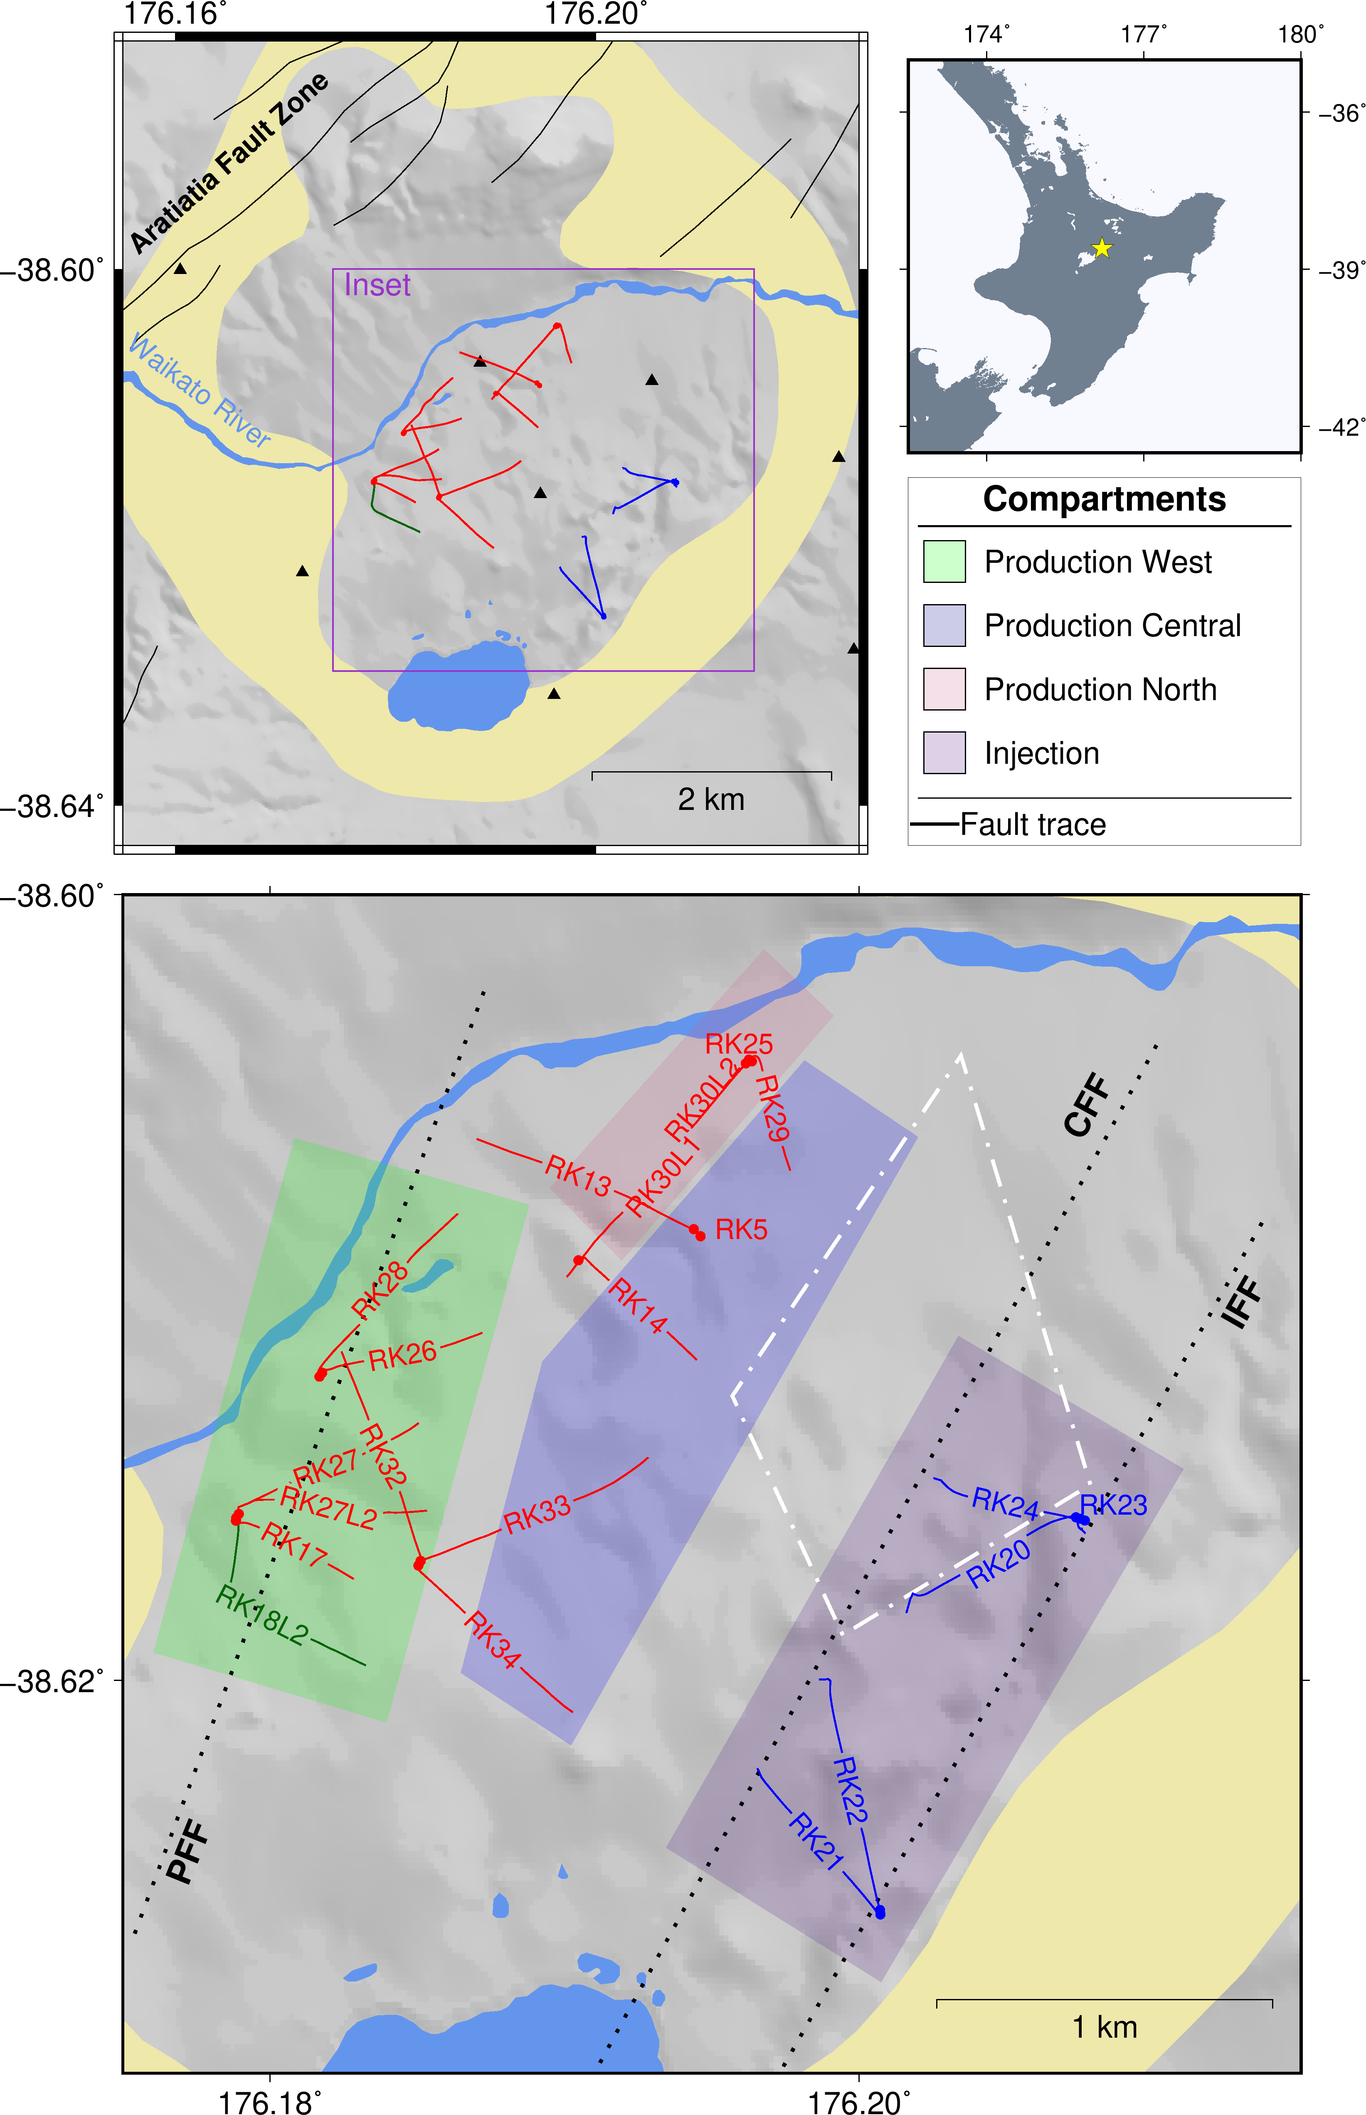
\includegraphics[width=0.75\columnwidth,height=\textheight,keepaspectratio]{Chapter_4_Rot/figures/merc_Rot_overview_inset/merc_Rot_overview_struct_inset_NI_compartments}
\caption[Overview of the Rotokawa geothermal field]{{
Overview of the Rotokawa geothermal field. The top right panel shows the
location of the field on the North Island of New Zealand (yellow star).
The top left panel shows the resistivity boundary of the field in yellow
and injection and production wells in blue and red, respectively. Solid
black lines are active faults. The lower panel shows a closeup of the
field, with the well names labeled and the three known faults (\acrshort{PFF}, \acrshort{CFF},
\acrshort{IFF}) shown as black dotted lines. The white dot-dashed line shows the
extent of significant seismicity from 2008-2012, as reported
by~\protect\citet{Sherburn_2015}. There are four known compartments in the Rotokawa
reservoir shown as colored polygons. Each is semi-isolated from the
others by either a \gls{permeability} contrast or impermeable barrier (i.e. a
fault). The production field comprises three compartments, the west,
central and north (green, blue and red, respectively). The injection
field is shaded in purple and is a separate compartment.
{\label{518273}}%
}}
\end{center}
\end{figure}

\subsection{Rotokawa resource development}
As with most of the Taupo Volcanic Zone geothermal fields, the existence of the Rotokawa resource was originally verified through a New Zealand government-funded drilling program starting in the 1960's \citep{cole1998rotokawa}. The first resource consent was granted to the Tauhara no. 2 Trust and various other entities in 1993 with electricity generation beginning in 1997 with the installation of the 24 \acrshort{MWe} \acrfull{RGEN} combined-cycle power plant \citep{legmann200330}. In 2000, Mercury NZ, Ltd. (then Mighty River Power) combined with the Tauhara no. 2 Trust to form the Rotokawa Joint Venture, which continues to oversee development at Rotokawa at present \citep{legmann200330}.

Prior to 2005, reinjection at Rotokawa was done at depths of \textless1000 m \citep{Sewell_2015} but was moved to greater depths (1000-3000 m) due to pressure buildup in the shallow injection zone \citep{McNamara_2016}. Additional resource consents were granted to the Rotokawa Joint Venture in 2007, prompting the drilling of more than ten additional wells (RK19-RK35) and culminating in the commissioning of the \acrshort{NAP} plant in 2010, bringing the total installed capacity at Rotokawa to 174 \acrshort{MWe} fed by 60,000--65,000 t/d of fluid from the reservoir \citep{McNamara_2016}. The additional information provided by the new wells allowed for significant improvements to the reservoir conceptual model detailed by \citet{Sewell_2015} and \citet{McNamara_2016}.

\subsection{Rotokawa operations changes} \label{rot_ops}
The dataset analyzed in this work spans the four years starting in 2012 and ending at the start of 2016. During this period, little new development was undertaken at Rotokawa, as the resource was adjusting to the significant increase in production associated with the startup of NAP in 2010. Changes in injection and production are therefore more subtle than those analyzed at the nearby Ngatamariki field for the same period, where drastic changes were associated with well \gls{stimulation} and power plant commissioning \citep{Clearwater_2015}. However, Mercury have identified a number of periods from 2012--2015 during which the character of seismicity may help address various outstanding questions about the nature of the reservoir:\selectlanguage{english}

\begin{table}
\centering
\begin{tabular}{cccc}
    {Field} & {Operation} & {Start} & {End}\\ \midrule
    Rotokawa & RK24 Injectivity Decline & 2012 & 2013\\
    Rotokawa & Switch of Injection: RK24-RK23 & June-2014 & July-2014\\
    Rotokawa & RK34 Drilling Losses & September-2014 & November-2014\\
    Rotokawa & Plant Shutdowns and Startups & 2012-2015 & 2012-2015\\
\end{tabular}
\caption[Rotokawa injection periods of interest]{{
Period of interest defined by Mercury for 2012--2015}}
\label{T1}
\end{table}

As is typically the case for produced reservoirs of any type (e.g. natural gas, oil, geothermal), seismicity at Rotokawa is caused predominantly by the injection, not the extraction, of fluids. This is because injection increases pore fluid pressure, thereby destabilizing fracture networks, whereas extraction achieves the opposite, although stress changes induced by the removal of reservoir volume are non-negligible in triggering earthquakes \citep{Segall_1989,2013}. For this reason, the periods defined by Mercury correspond predominantly to changes in injection operations. The first two, in Table \ref{T1}, correspond to a period of \gls{injectivity} decline in the dominant injection well RK24 (Figure \ref{518273}) due to an unknown cause. In response to the well's declining ability to accept injectate from the power plants, excess fluid was shifted to well RK23 (Figure \ref{518273}).

From September to November 2014, Mercury drilled an additional production well, RK34. At reservoir depths, the drilling operation incurred full fluid losses. Similar drilling losses induced a large number of seismic events during drilling in southern Ngatamariki \citep{j2019} and may have had a similar effect at Rotokawa. Finally, as noted by \citet{Sewell_2015WGC}, swarm-like behavior (which they defined as a day on which more than 15 events occurred) has been observed at Rotokawa in the past and is thought to be related to pressure perturbations induced by power plant shutdown and startup during regular maintenance operations.

The fluid injected at Rotokawa varies by application and between individual wells. For instance, during the drilling of RK34, the drilling fluid was composed predominantly of water at an ambient temperature of 10--20\textdegree C. During standard plant operations, the injectate at each injection well can be condensate (the product of cooling the steam used to turn the turbines), concentrated brine (brine with condensate removed) or some combination of these end members. During most of the period studied here, brine and condensate from NAP were injected into RK23-24, while the injectate from \acrshort{RGEN} was injected into RK20. Depending on the mixture, fluid entered the injection wells at a temperature between $\approx{}$ 40 and 130\textdegree C.

\subsection{Reservoir model}\label{model}
The behavior of the Rotokawa reservoir is dominated by three known NE-SW striking faults, each named for its location relative to the injection or production field. From east to west they are: the \acrfull{IFF}, \acrfull{CFF} and \acrfull{PFF} \citep{wallis2013} (Figure \ref{518273}). The existence and orientation of these faults is known from well cuttings that show vertical offsets in the top of the Rotokawa Andesite (and other units) between wells. The \acrshort{CFF}, for instance, is credited with a vertical displacement of nearly 400--500 m between the injection and production wells, while the \acrshort{IFF} and \acrshort{PFF} represent vertical displacements of 250--350 m \citep{wallis2013}. A number of independent datasets have been used to corroborate the presence of these faults, including tracer returns \citep{addison2015rotokawa,Addison_2017stanford}, pressure compartmentalization \citep{Quinao_2013stanford,Sewell_2015} and previous studies of microseismicity \citep{Sherburn_2015,Sewell_2015WGC}.

Large lateral pressure gradients within the Rotokawa reservoir indicate that it is made up of several discrete compartments that either have different permeabilities or are separated by structures that act as cross-strike flow barriers \citep{Quinao_2013stanford,Sewell_2015}. The major faults mentioned above act either as barriers between these compartments or as conduits for fluid flow within compartments. Slow or nonexistant tracer returns from injection to production indicate that the \acrshort{CFF} is such a barrier, isolating the injection compartment from each of the production compartments (Figure \ref{518273}). However, this isolation is not constant along the strike of the \acrshort{CFF} \citep{Addison_2017stanford}. Current modeling by Mercury suggests that a `leaky' connection exists between the main injection well, RK24 and the central production wells (RK5, RK14, RK29, blue polygon in Figure \ref{518273}), which provides pressure support to these production wells. This pressure support is not present in the western (4.2 MPa drawdown) or northern (3 MPa drawdown) production field compartments \citep{Quinao_2013stanford,Addison_2017stanford} (green and red, respectively in Figure \ref{518273}).

Strong pressure connection between the wells within the western production compartment suggests that the \acrshort{PFF} acts as an along-strike fluid conduit, transmitting pressure signals quickly to distances of up to a kilometer \citep{Quinao_2013stanford,Sewell_2015,McNamara_2016}. These pressure observations are well correlated with the geologic offsets observed in the well cuttings mentioned above \citep{wallis2013}.

There is less evidence to suggest what role the \acrshort{IFF} may play in reservoir behavior, as the only well completed to the east of this structure is RK23. Tracer was injected into RK23 in 2011, but issues with isotope breakdown rendered much of the test inconclusive. Bottom hole temperatures in RK20\slash24 are some 40\textdegree{C} hotter than in RK23, only $\sim$200 m away, suggesting some sort of lateral variation in reservoir properties between the wells (e.g. \gls{permeability}). However, some evidence suggests that there is also a significant pressure connection between all injection wells \citep{Quinao_2013stanford}. RK23 has traditionally accepted a smaller proportion of overall injection, so trends associated with changes there may be difficult to separate from the rest of the injection wells.

\subsection{Previous work}
The only previous studies of the seismicity at Rotokawa were conducted for the years 2008--2012 by workers at GNS Science and Mercury \citep{Sherburn_2015,Sewell_2015WGC}. These studies detailed a pattern of seismicity that shifted with time as the injection and production strategies evolved in response to field development and reservoir understanding. At of the end of 2012, \citet{Sherburn_2015} identified the currently-active area of seismicity as that bounded by the white, dot-dashed diamond shown in Figure \ref{518273}. This cluster of seismicity occurred at the approximate depth of the permeable zones in wells RK20, RK23 and RK24, which accounted for nearly all of the deep injection into the Rotokawa reservoir at the time. This cluster was inferred to be bounded to the northwest by the \acrshort{CFF} (Figure \ref{518273}), corroborating the evidence from tracer testing that fluid flow was impeded across the structure, thus allowing pressure buildup east of the fault and inducing seismicity \citep{Sherburn_2015,Sewell_2015WGC}. 

\citet{Sherburn_2015} and \citet{Sewell_2015WGC} cited the relatively modest \glspl{WHP_g} measured in the injection field (\textless1.5 MPa) as evidence for cooling-dominated, and not pressure-dominated, triggering of seismicity at Rotokawa. However, we feel that evidence is limited to support this claim, given that stress changes as low as $10^{-2}$ MPa have been shown to trigger seismicity in many settings \citep[][]{stein1999role,keranen2018induced}. As \citet{Sewell_2015WGC} noted, the large temperature gradients induced at the injection wells (\textgreater180\textdegree{C}) certainly produce stress changes of tens of MPa within 10-100s of meters of the well, especially when large volumes are injected over years \citep{stephens1982hydraulic}. Though the effect of cooling on fracture stability is complex \citep{Jeanne_2015deformation}, these cooling effects likely do dominate earthquake triggering close to the injection wells. However, the occurrence of seismicity beyond a $\sim${500} m radius and the lack of measured cooling at the production wells (including those that receive pressure support from the injection zone) indicate that other effects, including pore pressure increase and poroelastic stress transfer play a role in earthquake triggering \citep{Schoenball_2012}.

\section{Data and methods}
\subsection{Data}
As described in detail by \citet[][submitted]{j2019}, the Mercury seismic network covers an area of approximately 450 km$^2$ surrounding the Rotokawa and Ngatamariki geothermal areas. While most of the instruments are Mercury-owned 4.5 Hz Geospace GS-11D short-period geophones, we have also incorporated a number of stations operated by Contact Energy at their nearby Wairakei geothermal field, as well as three broadband instruments and one short-period instrument operated by the GeoNet national network (Chapter 2, Table 1). At any one time from 2012--2015, as few as 15 and as many 29 instruments were operational.

GNS Science, under contract with Mercury, provided the initial earthquake catalog used in this study. The raw waveform data were collected quarterly from Mercury's data loggers and supplemented by data from the aforementioned GeoNet stations. Events were automatically detected and located using the \textit{SeisComP3} software package \citep{Weber2007}. We threw out all events located \textgreater5 km outside the bounds of the Rotokawa resistivity boundary (yellow shaded area, Figure \ref{518273}), so that a total of 3225 microearthquakes of between M$_L$ 0.37 and 3.68 remained. We relocated these events using both the nonlinear location program \textit{NonLinloc} \citep{Lomax_2014} and the double-difference relocation software \textit{GrowClust} \citep{Trugman_2017} prior to undertaking the following analyses.

Production and injection well locations, temperatures, \glspl{flow_rate} and pressures were provided by Mercury.

\subsection{Matched-filter detection}
We used the matched-filter correlation detection approach described by \citet{j2019} to increase the number of events included in the GNS Science earthquake catalog mentioned above. This approach significantly increases the number of events detected without unduly increasing the rate of false detection and is well suited to detection at geothermal fields with many noise sources and dense clusters of small seismic events.

From the automatically-detected, GNS Science catalog we take only those events located within the field boundaries that have average pick residuals within one standard deviation of the mean pick residual for the entire catalog. Each of the resulting 3225 events was used as a `template' event. Each template consists of one-second-long waveforms, starting 0.1 seconds before the P-pick. We chose not to use the horizontal channels after inspection of the GNS automatic S-picks revealed a significant number of mis-picked arrivals. After applying an anti-aliasing filter, both raw and template waveforms were sampled at 50 Hz and filtered from 3.0 to 20.0 Hz.

To generate detections, templates were cross-correlated with continuous
data at a rate of 50 samples per second. At each sample, the cross-correlation
coefficients for each channel of data were summed to create the network detection statistic \citep{Shelly_2007}. A detection was recorded whenever the detection statistic exceeded a threshold value, which in this case was defined as the daily median absolute deviation (MAD) of the detection statistic multiplied by eight \citep[as suggested by][]{Shelly_2007}.

Duplicate removal was conducted by looping through all detections in order of descending detection statistic and removing detections within a user-defined time buffer of two seconds. We adopted two seconds for the time buffer following a visual review of template events that revealed numerous cases of near-repeating seismicity with inter-event times of 3--5 s.

Visual inspection of a subset of the detection waveforms showed that false detections occurred at a rate of approximately 1--3 false detections per day. However, there are too many detections to inspect them all manually. Therefore, we employ a sequence of thresholds based on the correlation between the template and detected waveforms in order to exclude lower-quality events, thus suppressing the number of false detections in our final catalog. These thresholds were applied during the location and magnitude calculation procedures described below. We visually inspected thousands of waveforms from the final catalog while manually picking first-motion polarities and did not encounter a single false detection.

\subsection{\textit{NLLoc} locations}
For each newly-detected event, P-picks were made at each channel included in the template via an automated workflow. For each station, the template and detected waveforms were correlated over a 0.2 second window centered at the detection time. Picks were recorded at the time corresponding to the highest correlation value within that window. If the correlation value of the template and detected waveform fell below 0.4, the pick was discarded. We then discarded those events with five or fewer picks. For the remaining events, we made automatic S-picks using the method developed by \citet{Diehl_2009} and modified by \citet{Castellazzi_2015}, a process detailed by \citep{mroczek_2019}. We located the remaining events with the nonlinear location program \href{http://alomax.free.fr/nlloc/}{\textit{NonLinLoc}} \citep{Lomax_2014} using a preliminary 1-D model computed using the program \textit{VELEST} \citep{Kissling_1994,sewell2017}(Chapter 2, Table 3).

\subsection{Magnitudes}
Magnitudes were calculated for each of the newly-detected events using an approach originally developed by \citet{Shelly_2016}. The specific approach used here is described in detail in \citet{j2019}, but relies on the assumption that the relative amplitude between a template event (for which a magnitude was calculated by GNS Science) and the detected event represents their relative moment. This relative moment can then be used to calculate the magnitude of the detected event.

We calculated relative amplitudes only when the cross-correlation coefficient between the template and detection exceeded 0.6 at any given station. For event pairs with a minimum of four common stations exceeding the correlation threshold, we calculated the relative moment as the median of the relative amplitudes, following \citet{Shelly_2016}. As the relative amplitudes are calculated from waveforms recorded at the same station, there is no need to remove the instrument response.

We used the template $M_{L}$ to calibrate the relative moment calculations from the method above and produce $M_{L}$ estimates for each detection. This was done by first converting the template $M_{L}$ to $M_{w}$ using the scaling relationship:

\begin{equation}\label{ristau_eq}
M_{L} = 0.88M_{w} + 0.73
\end{equation}

determined for locally detected, shallow New Zealand earthquakes \citep{Ristau_2009} and then converting to seismic moment using the well-known equation \citep{Hanks_1979}:

\begin{equation}
M_w = \frac{2}{3}\log_{10}M_{0} - 9
\end{equation}

Knowing the relative moment of the template event from the procedure outlined above, we then determined the relationship between the relative moments and actual moment which allowed us to convert relative moments to $M_w$ and then back to $M_L$ using Equation \ref{ristau_eq}. After applying this methodology, 28,414 events remained in our catalog.

\subsection{\textit{GrowClust} locations}
Finally, the entire catalog was relocated using the double-difference relocation program \textit{GrowClust} \citep{Trugman_2017} with differential travel times generated using the Python package \textit{hypoDDpy} \citep{lion_krischer_2015_18907} using a 1 s correlation window, a maximum time shift of 0.2 s and a minimum cross-correlation value of 0.6. The final 6479 double-difference relocations are shown in Figure \ref{349058}.

\subsection{$b$-value Calculation}\label{b-method}
The frequency-magnitude relationship for earthquake catalogs is a power-law distribution described by

\begin{equation}
\log{N} = a - bM
\end{equation}

\citep{gutenberg1942earthquake} where $a$ increases with the number of earthquakes in the catalog and $b$ describes the distribution of earthquake magnitudes above the catalog magnitude of completeness ($M_c$). We calculate $M_c$ for the catalogs presented here following the methodology of \citet{Wiemer_2000}. For a range of $M_c$ values, $a$ and $b$ are determined for our earthquake catalog and an idealized synthetic distribution constructed with the same $a$ and $b$ values. The absolute difference between the synthetic and measured distributions given by \cite{Wiemer_2000} is:

\begin{equation}
    R(a, b, M_{i}) = 100 - \Bigg(\frac{\sum_{M_{i}}^{M_{MAX}}|B_{i} - S_{i}|}{\sum_{i}^{}B_{i}}100\Bigg)
\end{equation}

where $B_{i}$ and $S_{i}$ are the observed and predicted number of events in a given magnitude bin, $i$. This residual is then minimized to find the most appropriate $M_c$ (figure \ref{Mc_calc}).

\begin{figure}[h!]
\begin{center}
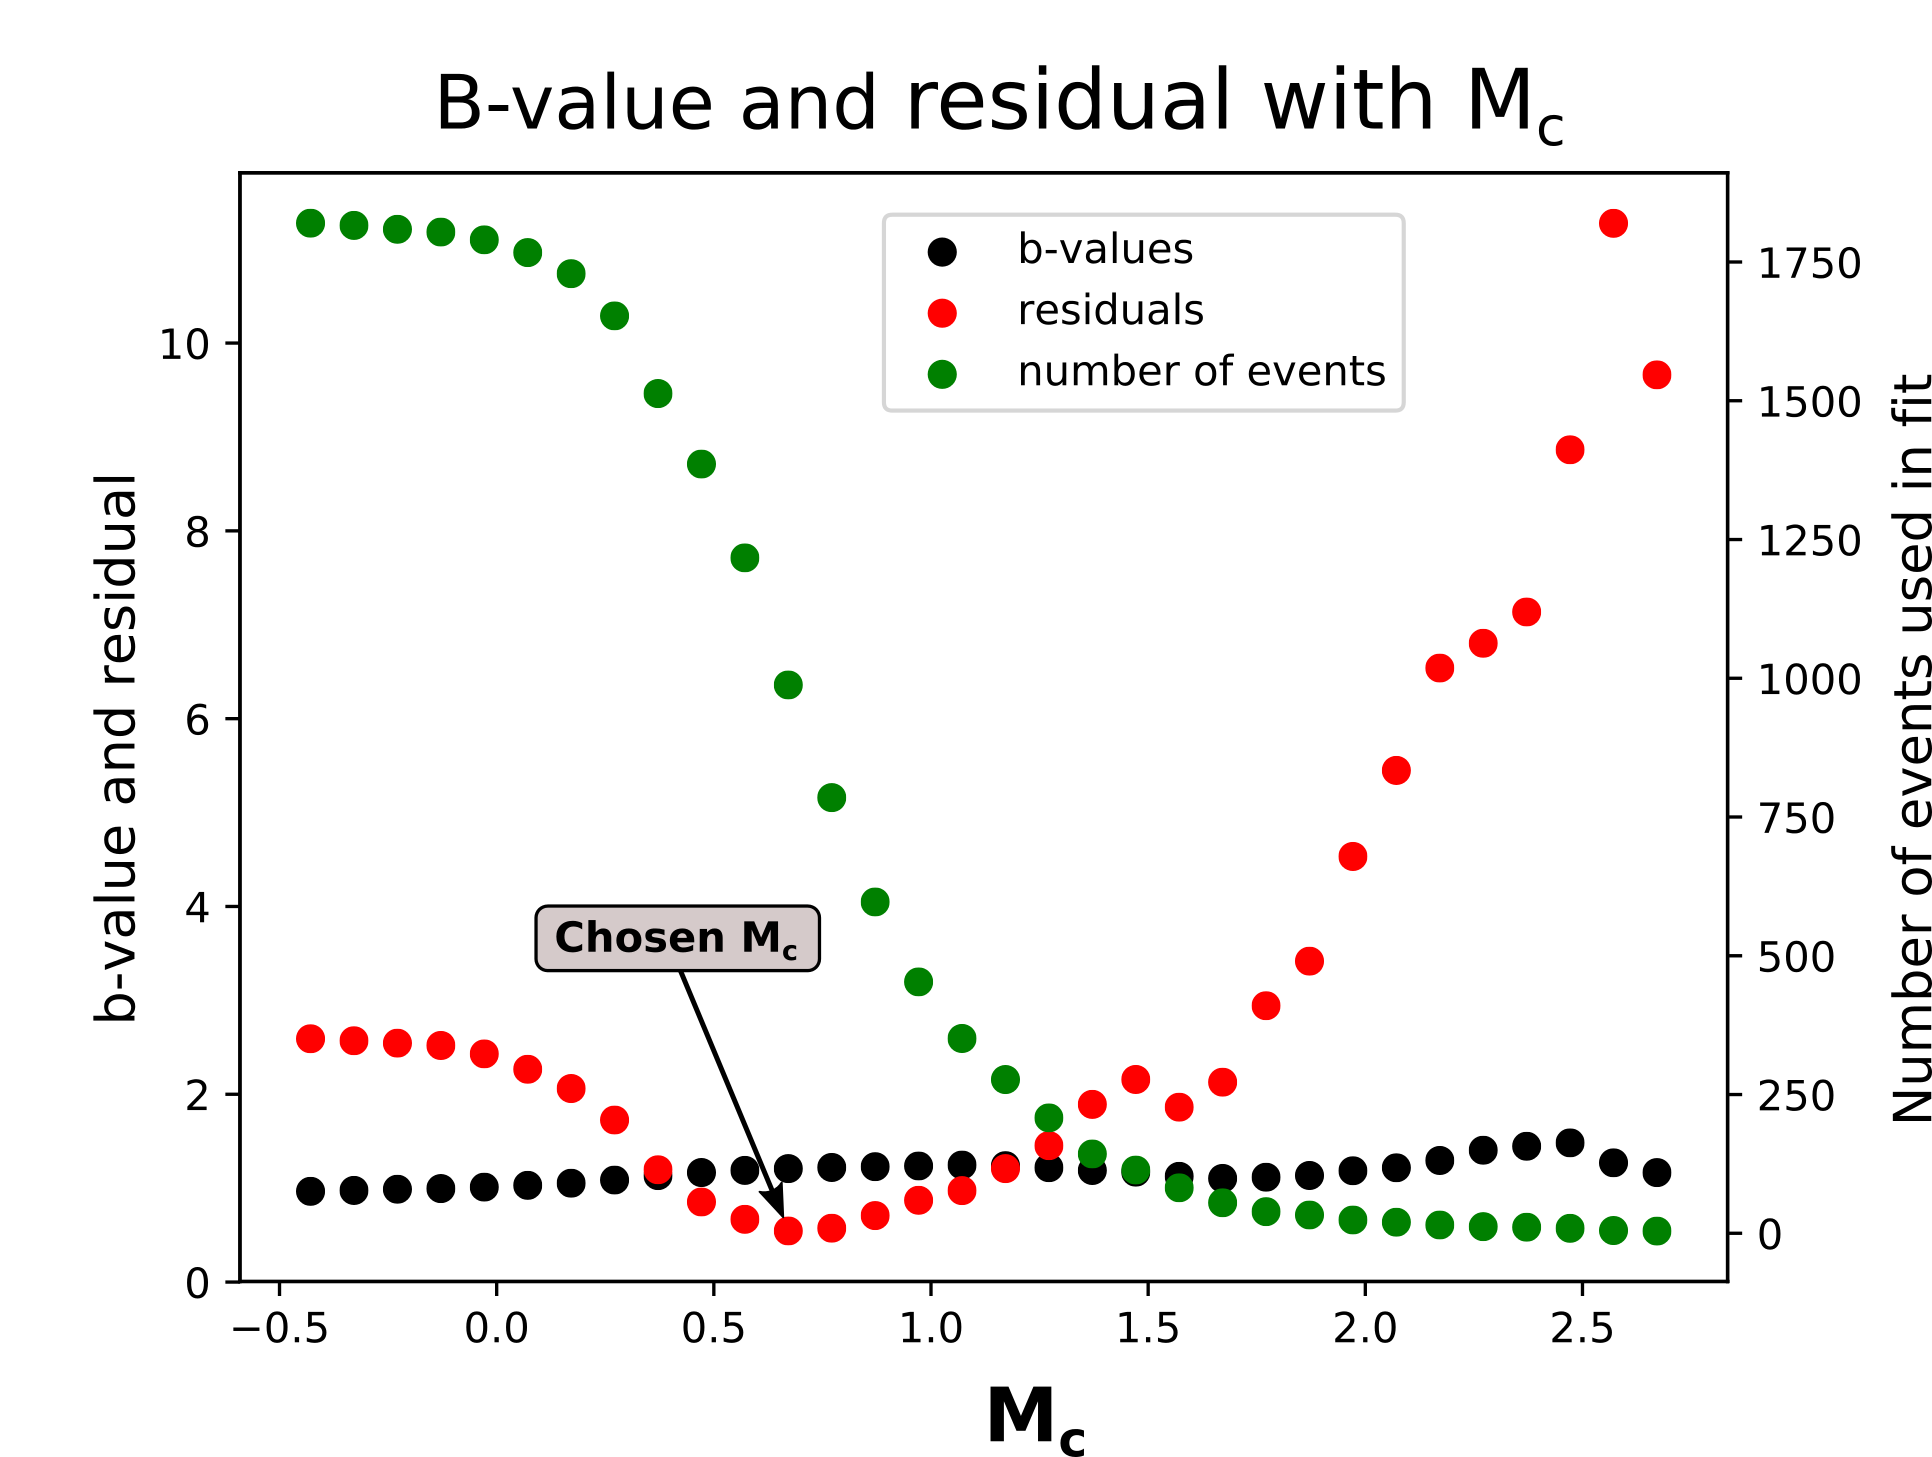
\includegraphics[width=1.00\columnwidth]{Chapter_4_Rot/figures/Mc_calc_wiemer_wyss_2000/Rot_IFF_wedge_wiemer_wyss_2000}
\caption[M$_{c}$ calculation]{{
Illustration of the magnitude of completeness calculation suggested by \citet{Wiemer_2000}. Red dots indicate the normalized, absolute difference between the observed and theoretical distribution of events for a given M$_{c}$ and $b$-value. Black dots are the calculated $b$-value and green shows the total number of events used for the fit at each magnitude of completeness.
{\label{Mc_calc}}%
}}
\end{center}
\end{figure}

We then map catalog $b$-value in space using the approach of \citet{Bachmann_2012}, wherein, for each event in the catalog (which they refer to as a `focus'), the nearest $n$ events are selected and $M_c$ is calculated for this subset. If the number of events above $M_c$ exceeds a threshold, the $b$-value is calculated and mapped to the focus event using the maximum-likelihood method \citep{aki1965maximum,shi1982standard}. \citet{Bachmann_2012} map the $b$-value for the 150 nearest events, with a threshold of 25 events greater than $M_c$. Here we use the nearest 300 events with a minimum threshold of 100 events above $M_c$.

One possible, yet poorly understood, complication in calculating $b$-values for our catalog arises due to the use of the matched-filter detection routine. A template event can only detect events with the same (or highly similar) location and fault plane solution. Therefore, if an event occurs in a location and/or with a focal mechanism solution for which there is no analog in the template catalog, it will go undetected. This may give rise to a bias in the final matched-filter catalog that would increase the uncertainty of M$_{c}$ and $b$-value. For the case of Ngatamariki and Rotokawa, although our template catalog was filtered to exclude events with high pick residuals (and therefore unreliable locations), we do not appear to have introduced any spatial bias, as shown by the similar distribution of template events relative to the raw, unfiltered catalog (see Chapter 2; Figure 2.3). Also, because the template events were drawn from the exact time span over which we conducted the correlation detection, we do not anticipate having introduced a temporal bias.

The final possible bias is that the template catalog is devoid of events having a particular focal mechanism. Assuming a lack of other biases, as stated above, the only way for this to have happened is if a particular mechanism occurred only at small magnitudes below the original amplitude-based detection threshold (M$_{c}\sim{0.7}$). However, due to the elevated pore-pressures present at actively-produced geothermal fields, we expect a scenario in which a variety of fracture orientations are activated, not only those corresponding to critically-stressed fractures, meaning that the potential focal solution space within the reservoir stress field should be relatively well-sampled in the template catalog. For a particular focal mechanism solution to be missing from the template catalog, it would likely need to have been \textless M$_{L}$ 0.7 and on a fracture oriented differently from the dominant NE-SW striking pattern in the reservoirs. It may be that such events correspond to new, tensile fractures induced by cooling-related contraction, which may produce such orientations and small sizes \citep{stephens1982hydraulic,Wiemer_1998} but we have difficulty envisioning another alternative scenario.

\section{Results}
\subsection{Locations}
The \textit{GrowClust} relocations of the final 6479 events are shown in Figure \ref{349058}. From a field-wide perspective, the location of seismicity has changed little from that presented by \citet{Sherburn_2015} and \citep{Sewell_2015WGC}. The area of seismicity identified in their studies is overlain on Figure \ref{349058} (black dot-dashed diamond) for context and broadly agrees with the extent of the densest seismcity in our catalog. Most events occur in the northeastern portion of the field, between the northern injection wells (RK20, RK23, RK24; Figure \ref{518273}) and the northern production wells (RK13, RK14, RK25, RK29, RK30; Figure \ref{518273}), with some events extending further towards the north and east. The northwest portion of the field, north of the Waikato River, as well as the southern injection zone (near wells RK21-22) correspond to areas of little seismicity. Within the area of densest seismicity, however, our catalog more clearly reveals subclusters and structure than previous studies, which identified only one uniform area of dense seismicity \citep{Sherburn_2015}.

\begin{figure}[h!]
\begin{center}
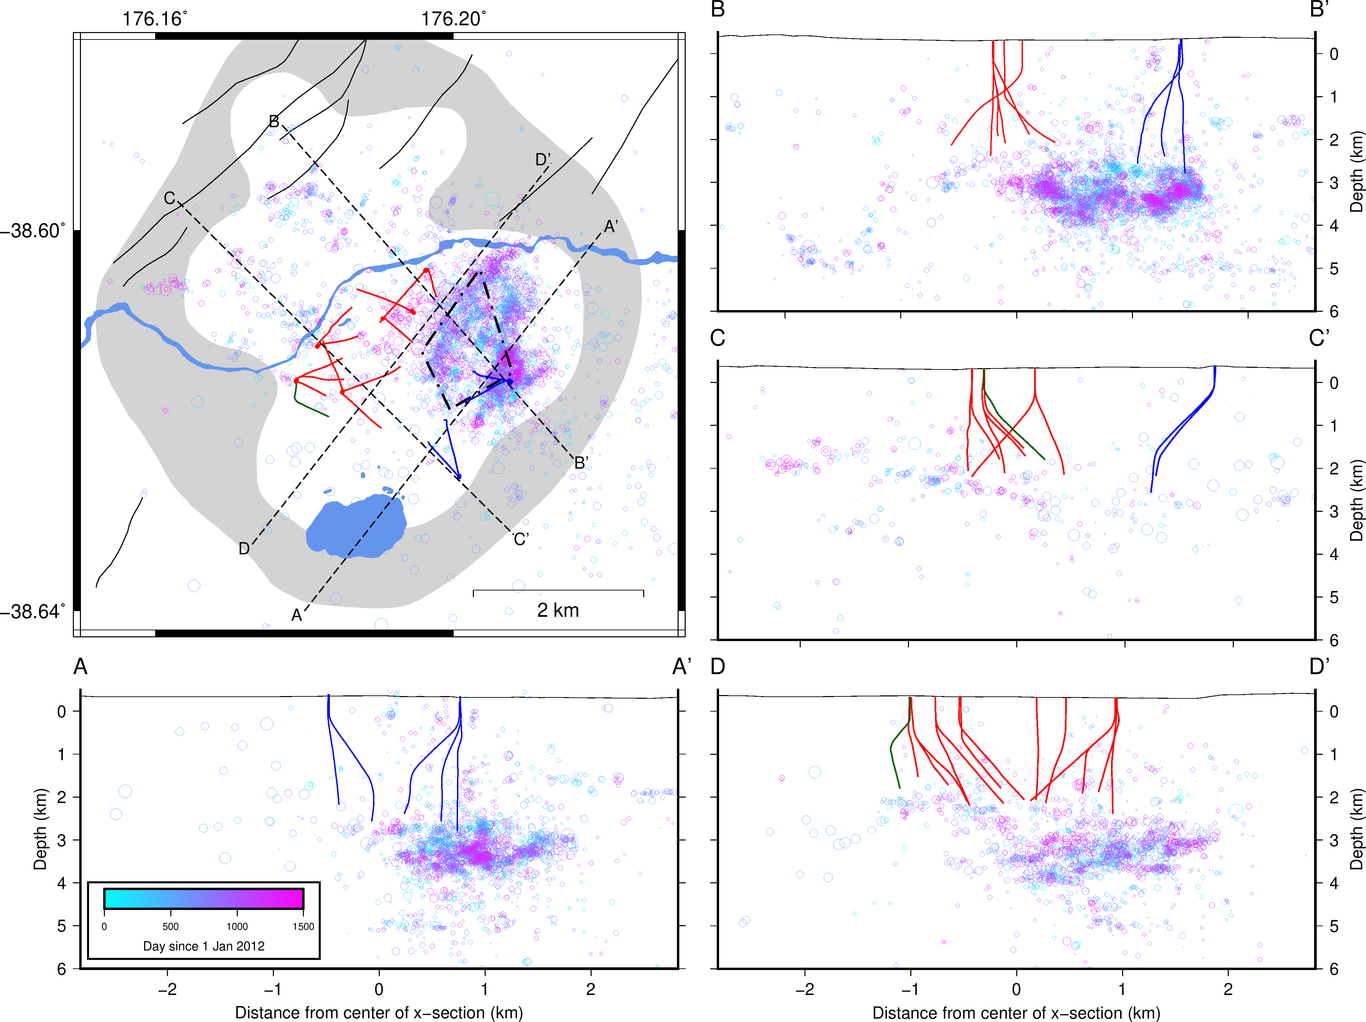
\includegraphics[width=1.00\columnwidth]{Chapter_4_Rot/figures/merc_Rot_dets_just_GC/merc_Rot_dets_just_GC}
\caption[Final Rotokawa seismic catalog]{{
Seismicity at Rotokawa for the years 2012-2015 colored by date of
occurrence. Blue events occurred earlier in the dataset and pink events
occurred later. Four cross sections are plotted to show the depth
distribution of seismicity and their surface projections are shown in
map view. The dot-dashed diamond indicates the area of dense seismicity
identified by \protect\citealp{Sherburn_2015,Sewell_2015WGC} for the 2008-2012 catalog.
{\label{349058}}%
}}
\end{center}
\end{figure}

\subsubsection{Location uncertainties}\label{loc_uncertainty}
There are obvious differences between the hypocenters presented here (2012--2015) and those presented by \citet{Sherburn_2015,Sewell_2015WGC} (2008--2012). While it is possible, that these location differences represent a real migration of seismicity, there are at least two other potential causes for this, which we will discuss in detail. The first is the location algorithm used to obtain the finalized, double-difference locations and the other is the significant uncertainty in the velocity structure at the geothermal fields.

In order to illustrate the potential contribution of the different location algorithms to the variations in earthquake hypocenters, we relocated a subset of an earlier GNS Science catalog containing only manual phase picks using two algorithms: \textit{GrowClust} (used in this study) \citep{Trugman_2017} and \textit{TomoDD} \citep{Sherburn_2015,Sewell_2015WGC,zhang2003double}. The locations for which are shown in Figure \ref{GNS_comp}. The velocity model used to obtain the GNS Science locations was an unpublished 3D model for Rotokawa \citep{Sherburn_2015}. For the \textit{GrowClust} locations, we located the catalog from scratch with \textit{NonLinLoc} \citep{Lomax_2014}, using the velocity model from \citet{sewell2017}, before relocating the catalog with \text{GrowClust}.\selectlanguage{english}

\begin{figure}[h!]
\begin{center}
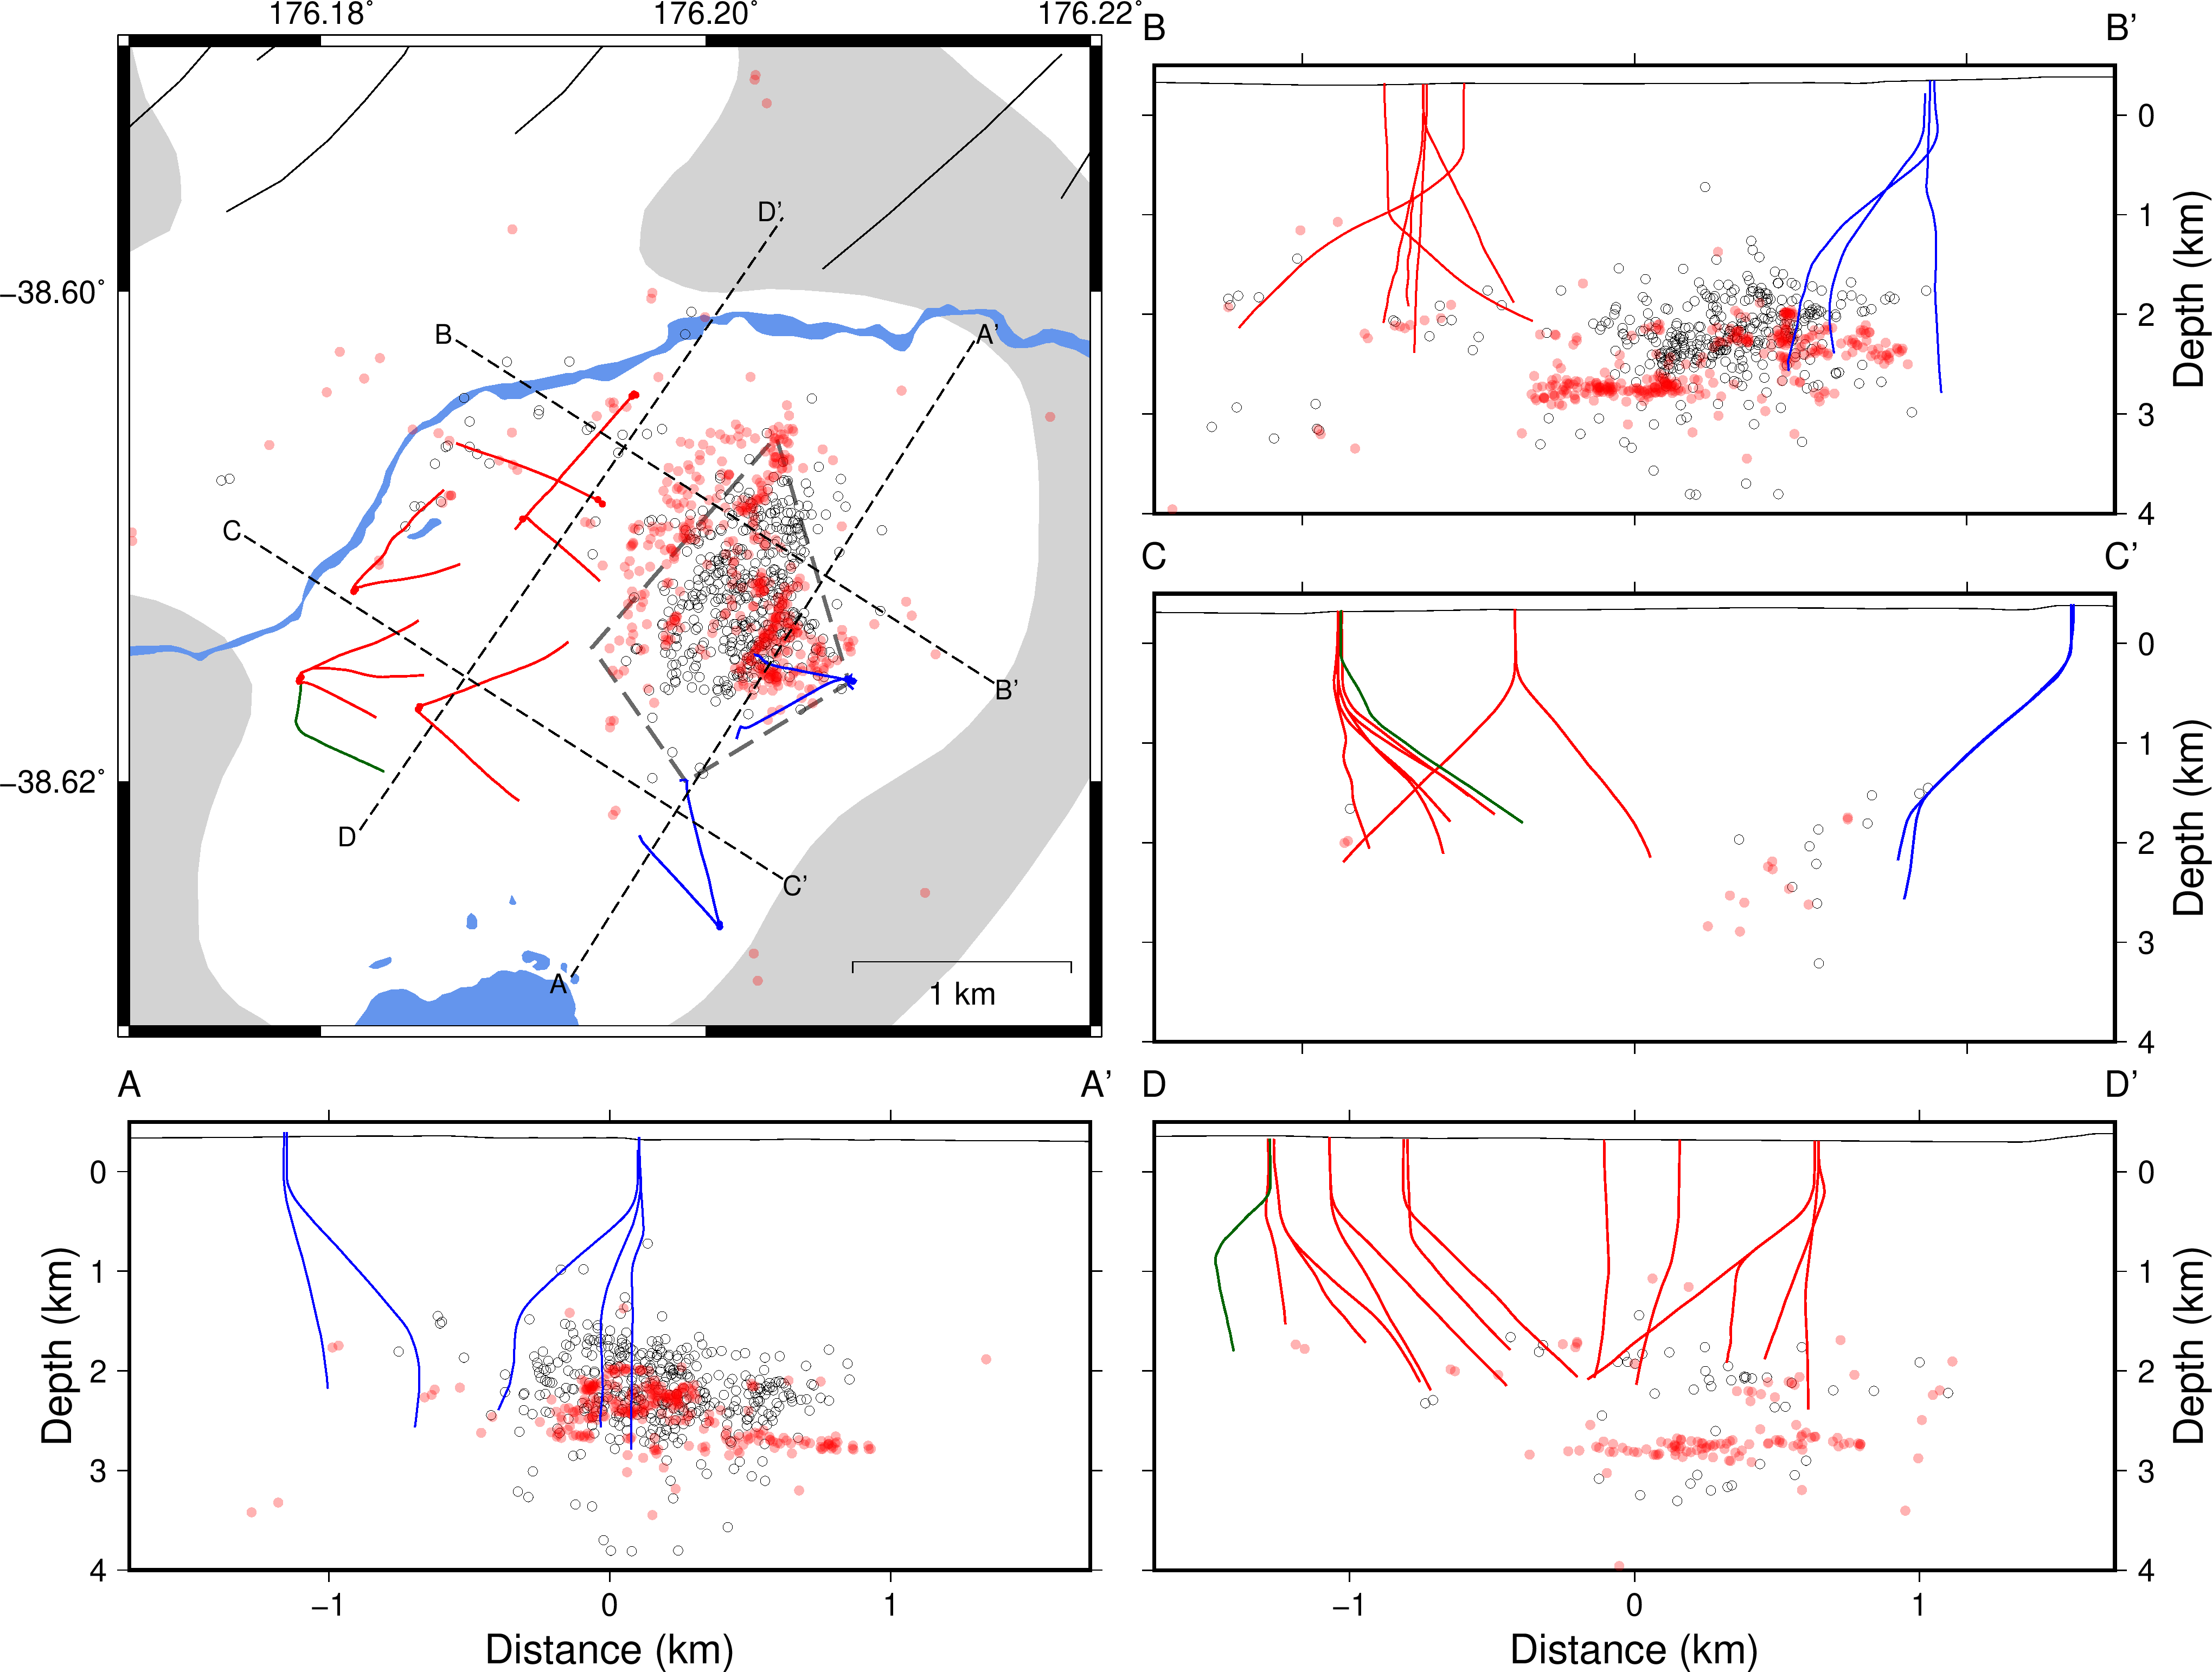
\includegraphics[width=0.98\columnwidth]{Chapter_4_Rot/figures/merc_Rot_GNS_comp/merc_Rot_GNS_GC-TomoDD}
\caption[\textit{GrowClust} vs \textit{TomoDD} relocation comparison]{{
GNS Science manual phase picks for 2012-2013, relocated with
\emph{GrowClust} (red circles), and by GNS Science with \textit{TomoDD} (black, unfilled circles). The dark gray, dashed diamond identifies the area of
active seismicity as of the end of 2012, defined by the \textit{TomoDD} locations of \citet{Sherburn_2015}. The \textit{GrowClust} hypocenters are more
tightly clustered, but occupy a larger overall footprint than the GNS
Science \textit{TomoDD} locations.
{\label{GNS_comp}}%
}}
\end{center}
\end{figure}

As stated above, the locations provided by GNS Science broadly agree with the depths of the major \glspl{feedzone} for the main injection wells (\textless2000 m bsl), particularly RK24, although a number of events occur at shallower depths (Figure \ref{GNS_comp}). Our \textit{GrowClust} locations cluster more tightly, especially in cross-section. Those events occurring nearest RK24 are in better agreement with the depth of the \glspl{feedzone} than the \textit{TomoDD} locations. In map view, these events also define a structure striking NE-SW, consistent with the regional trend and perhaps associated with the \acrlong{IFF}, previously inferred from stratigraphic offsets between the three main injection wells RK20, RK23 and RK24, which were all drilled from the same wellpad \citep{Sewell_2015}.

While the \textit{GrowClust} locations are more consistent with known structures and \gls{feedzone} depths in the deep reservoir, it is nevertheless difficult to state with certainty that they are the `correct' locations. Figure \ref{GNS_comp} simply serves to show that, using the same data, variations in velocity model and location algorithm can produce hypocenters that may yield different interpretations. We are conscious of these uncertainties but continue with the analyses of the \textit{GrowClust} locations.

\subsection{Magnitudes}
In Figure \ref{848333}, we show the frequency-magnitude distribution for the GNS template events (dashed) and final detected events (solid) for which we calculated a $b$-value of $\sim${1.09}$\pm$0.02, comparable to $b$-values in areas of hydrothermal activity worldwide, and similar to those calculated at the Ngatamariki geothermal field, located $\sim${7} km to the north (Figure \ref{848333}B) \citep[e.g.][]{Bachmann_2012,Wiemer_1997,Dinske_2012,j2019}. In areas of active volcanism, as well as in both hydrocarbon extraction and geothermal settings, $b$-values far exceeding 1.0 are reported  \citep{Dinske_2012,Shapiro_2011}. In general, $b$-values above 1.0 have been attributed to the presence of fluids, high pore-fluid pressures and material heterogeneity. Elevating the pore pressure allows fractures to fail that are not optimally-oriented in the local stress field. These fractures experience smaller differential stress than those which are critically stressed, and will therefore produce smaller-magnitude earthquakes when they fail \citep{Bachmann_2012}. It has also been suggested that the presence of a strong thermal gradient (e.g. related to an intrusion or injection of cold water) could aid in development of small, tensional fractures \citep{Warren_1970}, thereby increasing the population of small fractures, which can only fail in small-magnitude events. Both the elevation of pore pressure and the application of a strong thermal gradient may increase the frequency of small-magnitude seismic slip and therefore raise the $b$-value above naturally-occurring values (i.e. $\sim$1.0).

Figure \ref{848333}B shows the $b$-value at Rotokawa in comparison to the values for the two clusters of seismicity at the Ngatamariki geothermal field calculated by \citet{j2019}. The $b$-value at Rotokawa is most similar to that of the southern injection zone at Ngatamariki, likely because both areas encompass major structures \textgreater1 km in length that are able to accommodate larger-magnitude earthquakes. As described by \citet{j2019}, the high $b$-value in northern Ngatamariki is likely related to intense intrusive-related alteration, which has produced a fracture population that is relatively devoid of large structures, limiting the likelihood of producing larger events.\selectlanguage{english}

\begin{figure}[h!]
\begin{center}
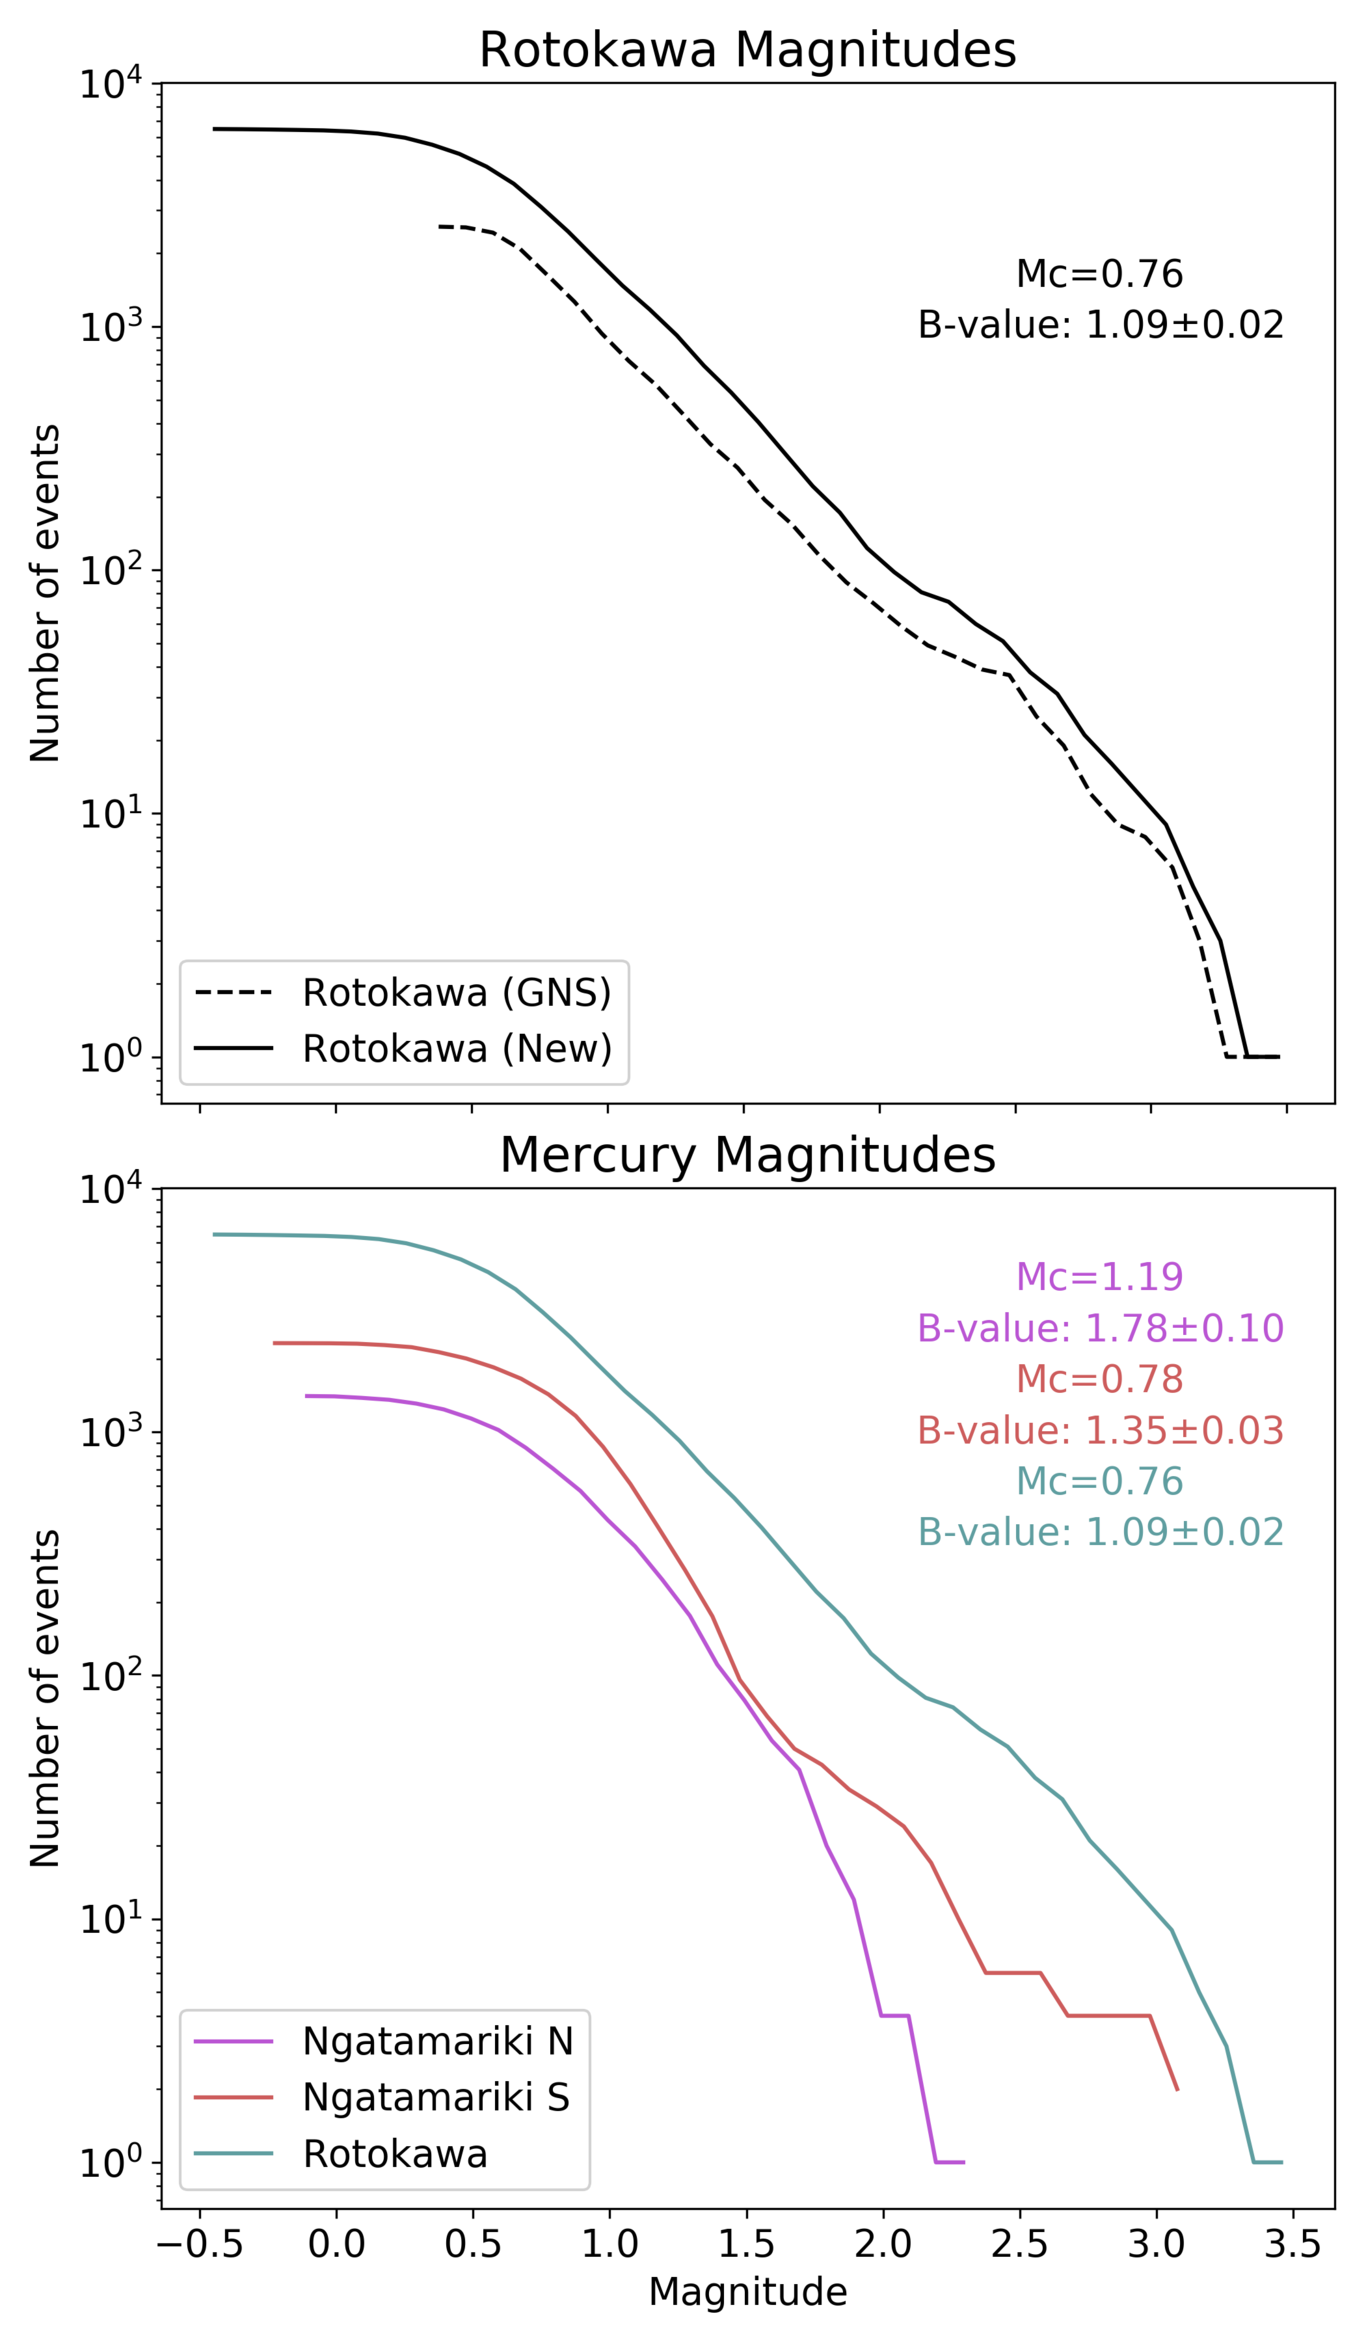
\includegraphics[width=0.70\columnwidth]{Chapter_4_Rot/figures/Rot_cumulative_bval_plot/Merc_cumulative_bval_all_2-panel}
\caption[Catalog frequency-magnitude distributions]{{
Top panel: Frequency-magnitude distributions for the GNS (dotted) and
matched-filter-detected (solid) catalogs at Rotokawa from 2012-2015. The
calculated magnitude of completeness and $b$-value are noted in the top
right for the matched-filter catalog. Bottom panel: Frequency-magnitude
distributions compared for Northern Ngatamariki, Southern Ngatamariki
and Rotokawa. The Mc and $b$-value for each catalog is noted in the top
right, consistent with the catalog order in the legend.
{\label{848333}}%
}}
\end{center}
\end{figure}

\subsection{$b$-value mapping}
Figure \ref{610416} shows $b$-value in map view and cross-section. There are no immediately-evident spatial trends in $b$, which instead shows a complex, heterogeneous distribution varying from 0.4 to nearly 2.0. $b$-values of \textgreater1.5 are found throughout the reservoir, including north of the Waikato river, where no production occurs, and a small center of elevated values ($b\approx$1.8) roughly 500 m north of injection well RK23.

\begin{figure}[h!]
\begin{center}
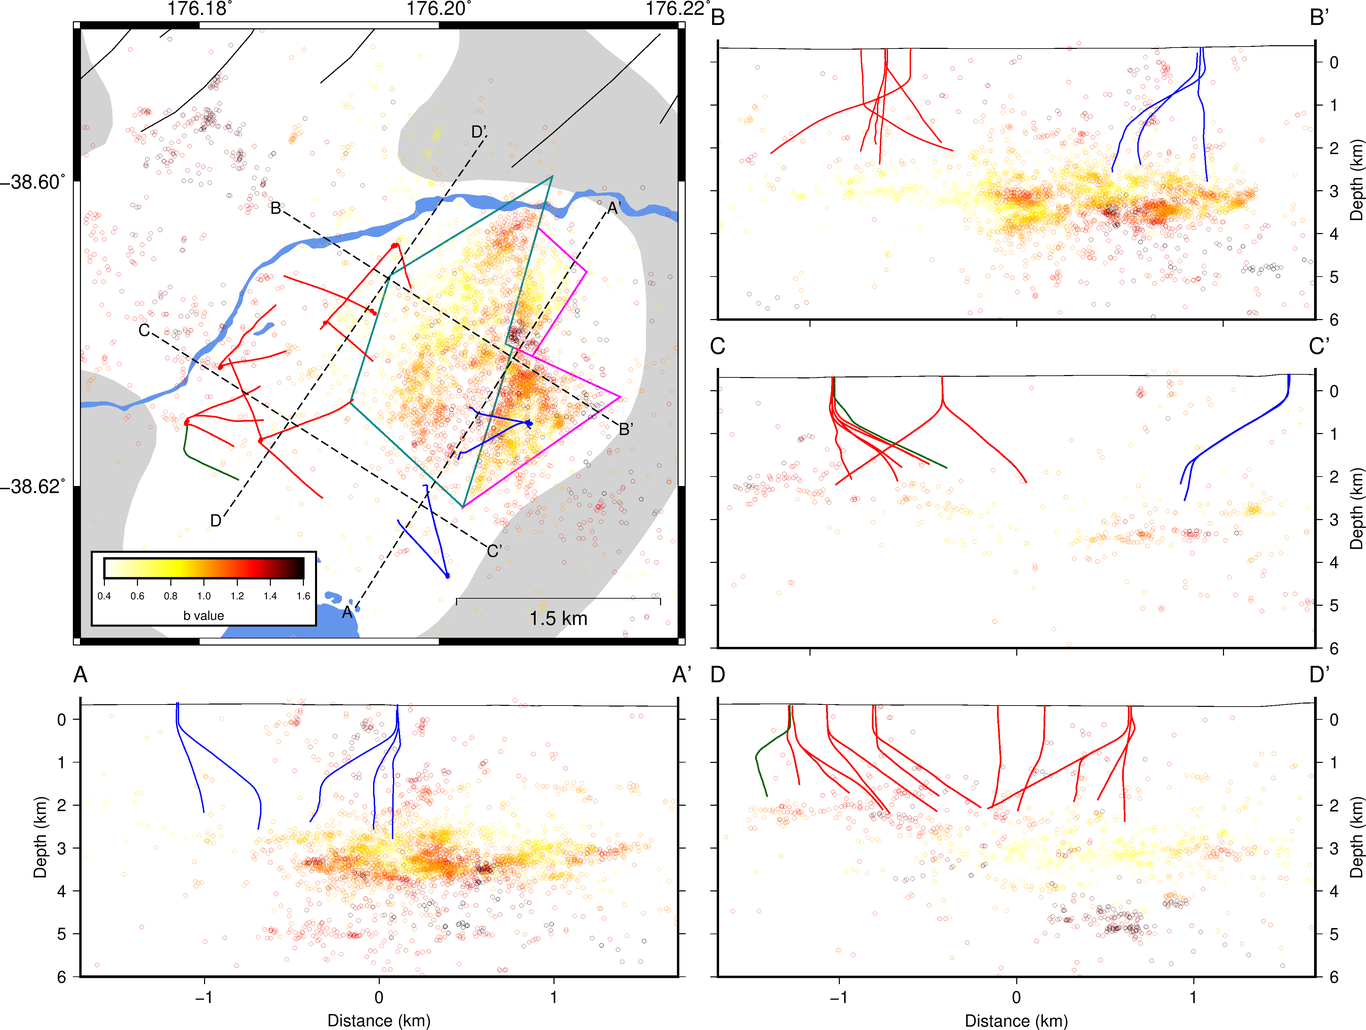
\includegraphics[width=1.00\columnwidth]{Chapter_4_Rot/figures/merc_Rot_dets_just_GC_bval_map/merc_Rot_dets_just_GC_bval_map_PS_max300_min100_maxlike_comps}
\caption[Rotokawa $b$-value map]{{
Spatial variation in~\emph{b}-value at Rotokawa. Events are colored by
$b$-value, calculated using the nearest 300 events, provided there are at
least 100 events greater than the M$_{c}$. The western (green polygon), northeastern (coral polygon) and southeastern (pink polygon) compartments are defined from hypocentral locations and will be relevant to the following discussion.
{\label{610416}}%
}}
\end{center}
\end{figure}

\section{Discussion}
\subsection{Compartmentalization}
As shown in Figure \ref{518273} and discussed in Section \ref{model}, the Rotokawa reservoir is known to be broken into a number of compartments, at least three in the production field and one in the injection field. Patterns in seismicity are of little use in delineating the borders of the production field compartments because relatively few earthquakes occur in that portion of the field. However, we think that our relocations (Figs. \ref{349058} and \ref{935417}) allow for further constraint on the location of the Central Field Fault and Injection Field Fault, and may provide evidence for previously unidentified subcompartments within the injection field.

There are at least two NE-SW-striking sub-linear features revealed by this catalog, outlined and labeled in bold red in Figure \ref{935417}B. One feature lies between the injection and production fields, taking on an arcuate shape, concave towards the southeast. This structure likely defines the \acrshort{CFF} as it sits between the injection field and the central production compartment, as previously modeled by \citet{wallis2013}. The other structure strikes NE-SW between wells RK20/24 and well RK23, and extends towards the northeast. We therefore interpret this to be the \acrshort{IFF}, again due to the consistency of its location with known geologic and temperature offsets. The \acrshort{IFF}, specifically, was not previously imaged by microseismicity, nor has the offset between what appear to be \acrshort{CFF}-related and \acrshort{IFF}-related events \citep{Sherburn_2015} been previously identified. We suggest three possible reasons for this:
\begin{itemize}
    \item One, we are able to more clearly define structures as a result of the larger number of events in our catalog;
    \item Two, the change in algorithm used for the double-difference relocation (\textit{GrowClust}, in our case) was more stable in the presence of noisy data than \textit{TomoDD} (see Section \ref{loc_uncertainty});
    \item Three, the location changes may actually reflect reservoir-scale changes in \gls{permeability} and fluid flow from 2012 through 2015.
\end{itemize}
We cannot rule out the possibility of large-scale migrations in the seismically-active portion of the reservoir. For example, deepening of seismicity has been observed at The Geysers geothermal field \citep[e.g.][]{Mart_nez_Garz_n_2014,Jeanne_2015tensor}. However, as shown in Figure \ref{GNS_comp}, changing only the data processing and algorithm for a single set of phase picks is enough to produce significant changes in the final locations. In addition, the \textit{GrowClust} locations using GNS Science manual phase picks (red dots, Figure \ref{GNS_comp}) resemble our final locations using automatic and cross-correlation-derived picks (Figure \ref{349058}), with two separate clusters of seismicity aligned NE-SW. The means that the revealed structures are independent of data quality, given that the manual picks are more precise than our automatic picks. Finally, the two separate structures make sense geologically, given the known locations of both the \acrshort{CFF} and \acrshort{IFF} from well cutting offsets. For these reasons, we prefer our locations to those published previously by GNS Science \citep{Sherburn_2015}.

A third potential structure is outlined in dotted red striking NW-SE (Figure \ref{935417}). On visual inspection, this feature is less obvious than those of the \acrshort{CFF} and \acrshort{IFF} and we therefore assign less confidence to its existence. Furthermore, no major cross-strike (NW-SE) structures have been identified from offsets in well cuttings. However, along-strike variations in pressure drawdown and tracer returns do indicate that the reservoir is likely divided not only by NE-SW-striking structures, but NW-SE-striking structures as well \citep{Sewell_2015,Quinao_2013stanford}. Specifically, the contrast between the \textgreater4 MPa drawdown in the western production field (green box, Figure \ref{518273}) and the 3 MPa drawdown at the northern production wells (red box, Figure \ref{518273}) suggests the existence of NW-SE structures.

The following analysis is based on the hypothesis that pressure differentials between compartments may exhibit as variations in seismic characteristics. Therefore, we have divided the area of densest seismicity into three potential compartments bounded loosely by the inferred locations of the major faults and the potential NE-SW structure mentioned above (Figures \ref{610416} and \ref{935417}). The light green polygon in Figure \ref{935417}B will be referred to as the western compartment and the coral and pink polygons will be referred to as the northeastern and southeastern compartments, respectively. These divisions are based on hypocentral locations only and constitute potential compartments that have not been identified previously.\selectlanguage{english}

\begin{figure}[p]
\begin{center}
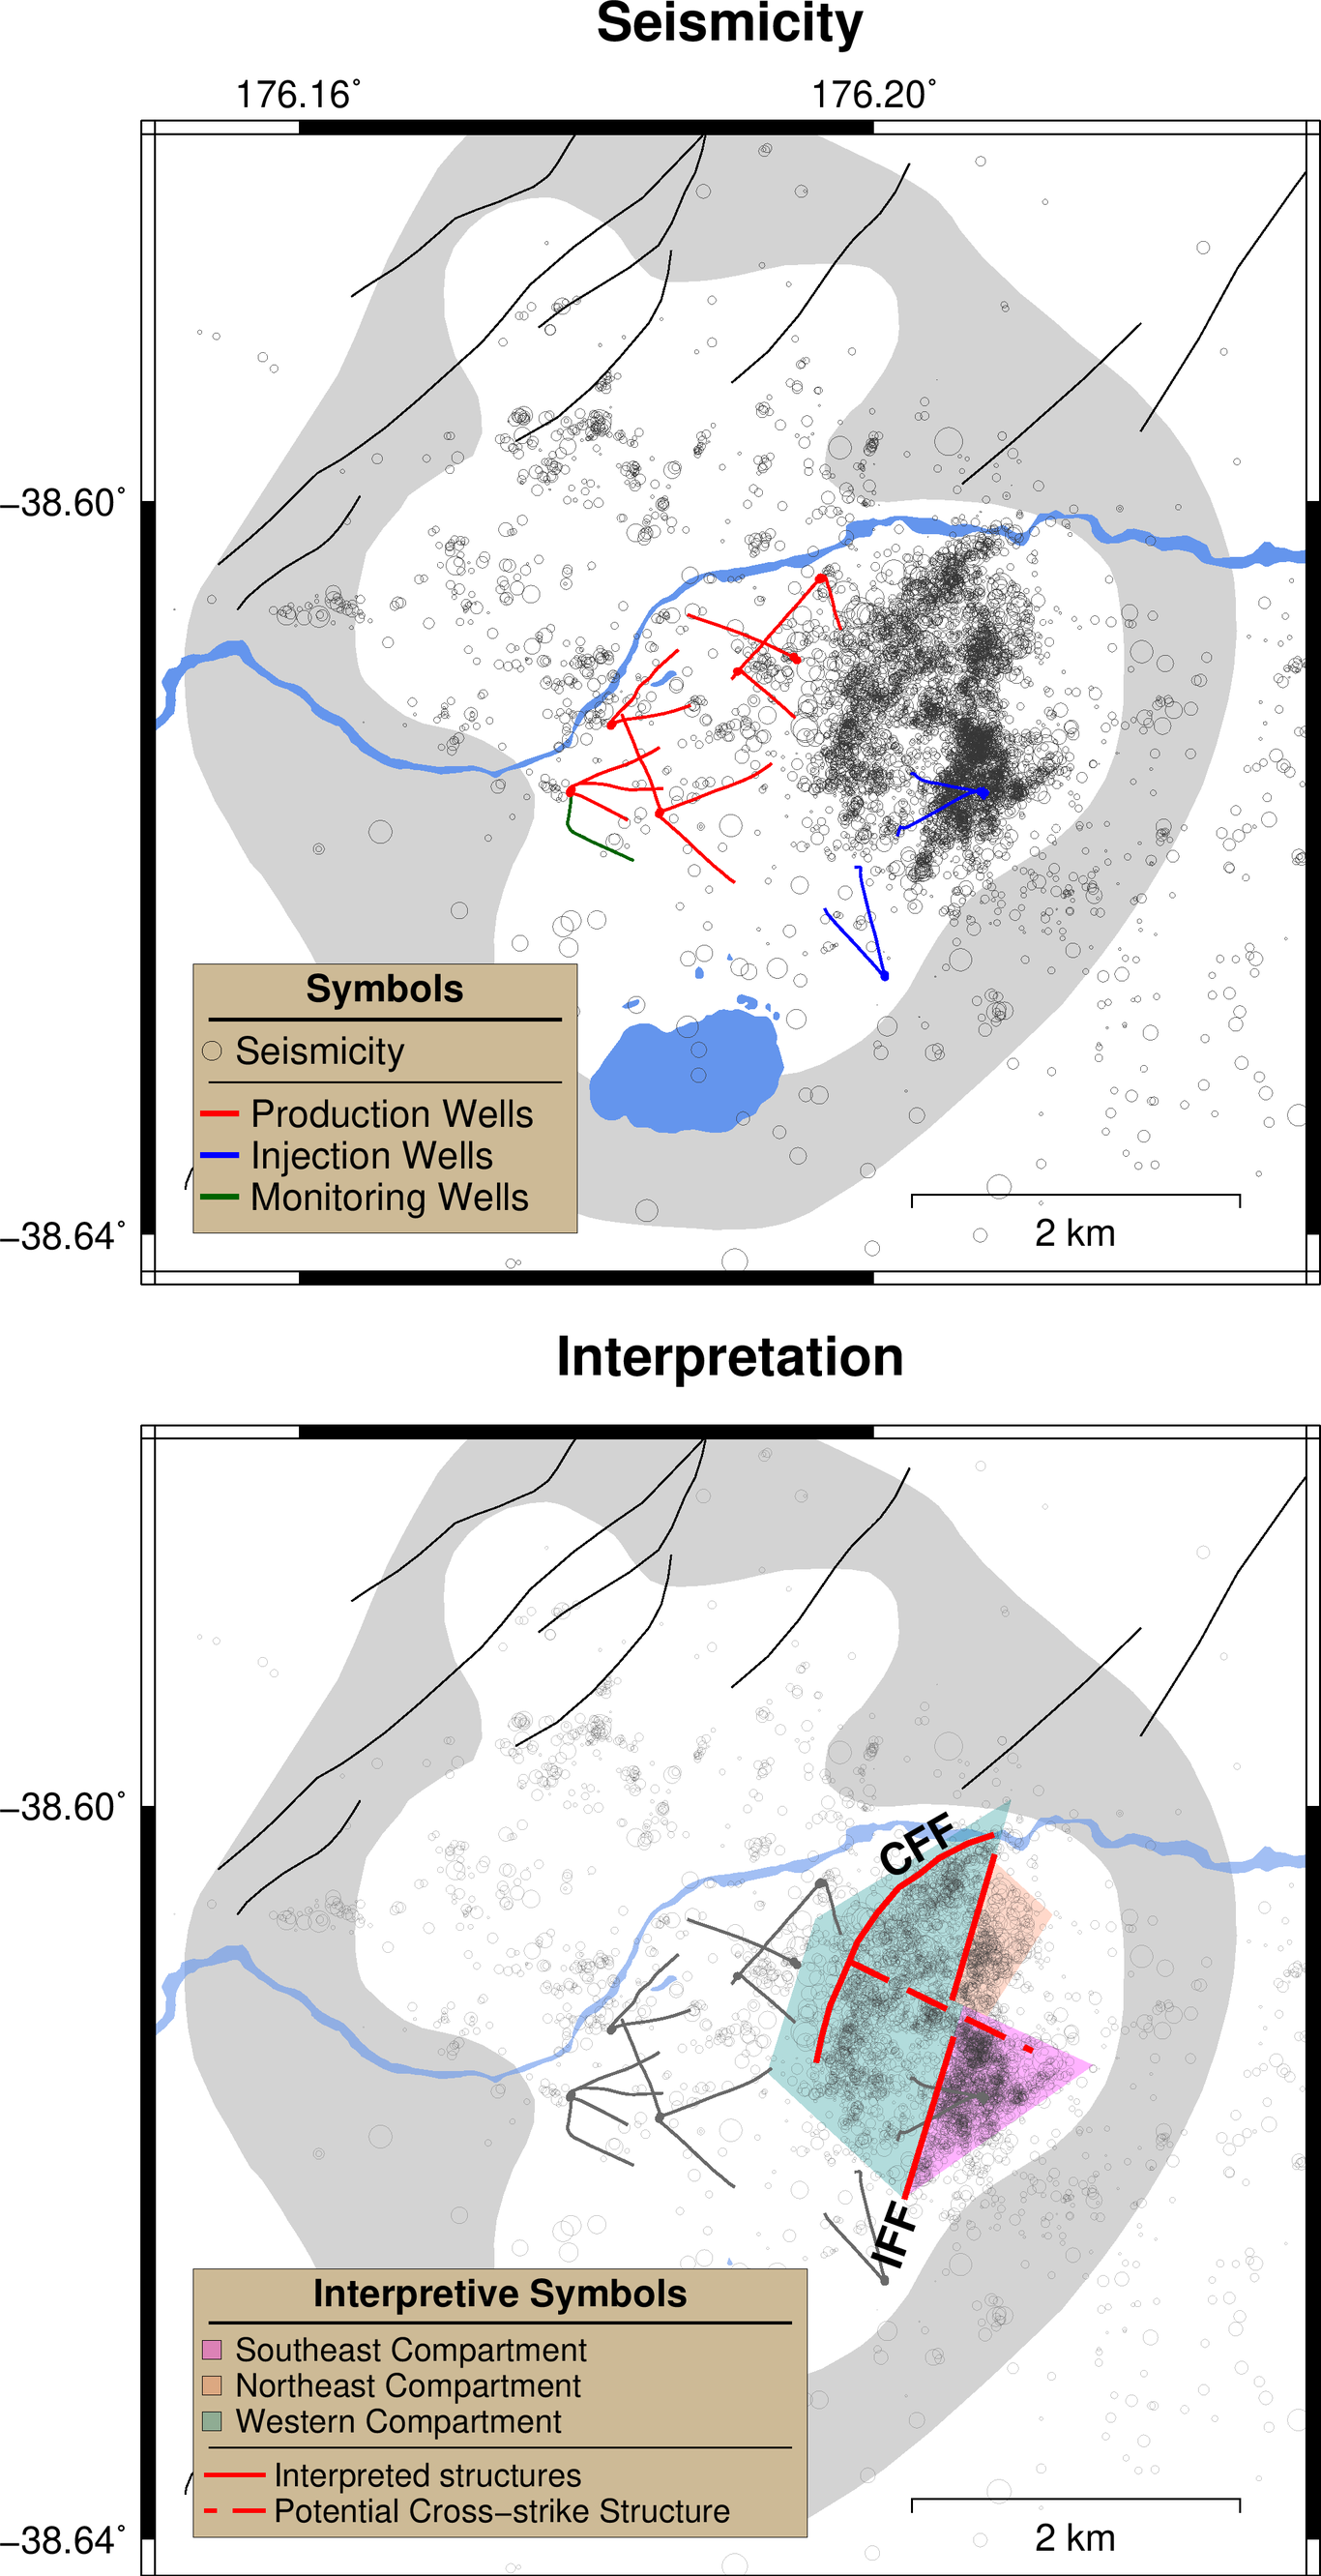
\includegraphics[width=0.66\columnwidth]{Chapter_4_Rot/figures/merc_Rot_dets_GC_boundaries/merc_Rot_dets_GC_boundaries_labs}
\caption[Reservoir compartments inferred from seismicity]{{
Seismicity at Rotokawa from 2012-2015, relocated with \textit{GrowClust}. The top
panel shows seismicity as black circles, scaled to each earthquake's
magnitude (as in Figure~{\ref{349058}}). The bottom
panel shows our interpretation of reservoir structure from the location
of seismicity (red lines). These structures may define reservoir
compartments (colored regions). The location and orientation of the
Central Field Fault and Injection Field Fault (solid red) are well
constrained from seismicity. In addition, the dotted red line indicates
the location of a possible cross-strike structure north of the injection
field, which may contribute to further injection-field
compartmentalization.
{\label{935417}}%
}}
\end{center}
\end{figure}

\subsection{Compartment characteristics}
For a first-order view of the properties of seismicity in the compartments defined in Figure \ref{935417}, we plot the cumulative number of events as well the normalized number (dividing by the total) of events in each (Figure \ref{599295}a-b) as well as their respective frequency-magnitude distributions (Figure \ref{599295}c). Panels a and b do not reveal striking differences in the rate of seismicity between compartments, with the exception of an increased rate of events in the northeast compartment (coral-colored) relative to the others at the end of 2012, which will be investigated in Section \ref{temporal}. However, panel c reveals a significant variation in $b$-value between compartments. While the western and northeastern compartments have $b$-values of 0.93$\pm$0.05 and 1.03$\pm$0.03, respectively, the $b$-value in the southeast compartment is markedly higher (1.16$\pm$0.03). Given that the southeast compartment is the closest to the main injection wells (RK20, RK23 and RK24), this may suggest that the $b$-value at Rotokawa is proportional to pore-fluid pressure, which is most elevated near injection wells. A similar, but stronger, effect was observed by \citet{Bachmann_2012} at the Basel injection site in Switzerland, who found $b$-values \textgreater2.0 near the injection interval, albeit for \glspl{WHP_g} (30 MPa) an order of magnitude higher than observed at Rotokawa (\textless{2} MPa) \citep{haring2008characterisation}.

To test the significance of the compartment $b$-value variations, we use the approach of \citet{utsu1999representation} where the probability that any two sub-catalogs come from the same population is given as \cite{Wiemer_1998}:

\begin{equation}
    P\approx{}\exp(-dA/2 - 2)
\end{equation}

Here, $dA$ is the difference in the Akaike Information Criterion for the null hypothesis (i.e. both catalogs have the same $b$-value) and the hypothesis that their $b$-values are distinct such that:

\begin{equation}
    dA = -2\ln{N} + 2N_{1}\ln{N_{1} + N_{2}b_{1}/b_{2}} + 2N_{2}\ln{N_{1}b_{2}/b_{1} + N_{2}} - 2
\end{equation}
 where $N_{1}$ and $N_{2}$ are the number of events in the two catalogs being compared, $N$ is $N_{1} + N_{2}$ and $b_{1}$ and $b_{2}$ are the $b$-values of the individual catalogs.
 
Using this method, we find that elevated $b$-value in the southeast compartment is significant at the 99.98\% level or greater relative to both the western and northeastern compartments.

\begin{figure}[p]
\begin{center}
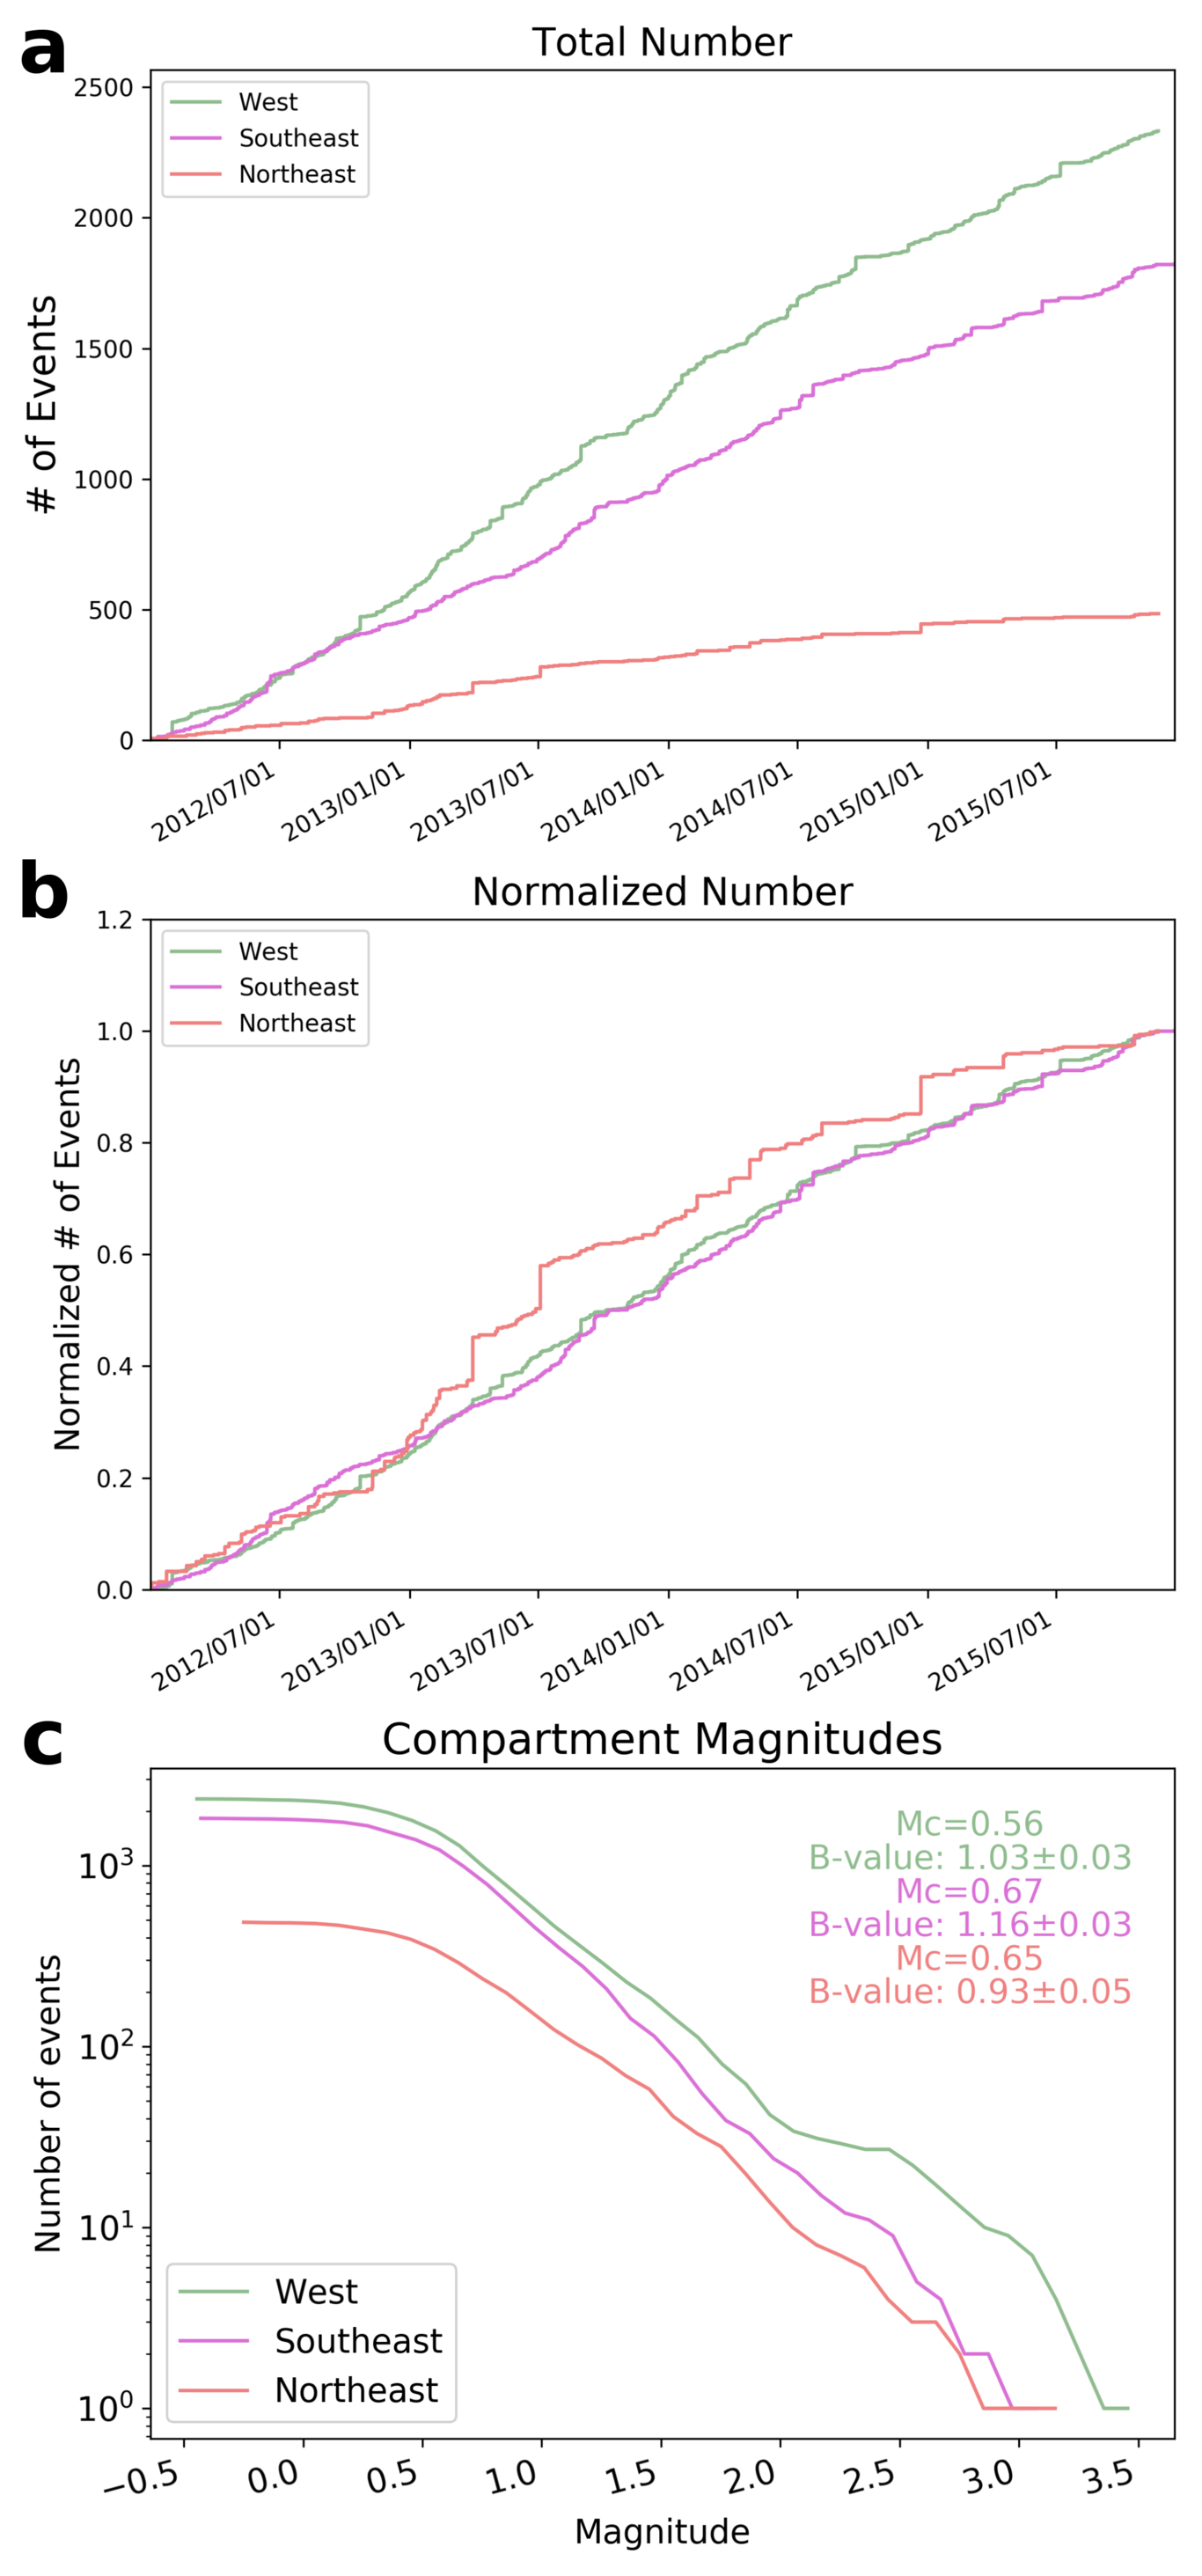
\includegraphics[width=0.67\columnwidth]{Chapter_4_Rot/figures/Rot_bval_compartments/Rot_dets_compartments_w_mags_max-like_labels}
\caption[Compartment characteristics of seismicity]{{
a) Total and b) normalized cumulative number of earthquakes in each of
the three compartments defined in Figure~{\ref{935417}}
. c) Frequency-magnitude distributions for each of the compartments.
{\label{599295}}%
}}
\end{center}
\end{figure}

\section{Temporal variations in seismicity and injection parameters}\label{temporal}
Characteristics of seismicity are used by geothermal operators to supplement more traditional, well-based pressure and temperature measurements for reservoir management. At Rotokawa, microseismicity has been used to constrain the location of major structures such as the \acrshort{CFF} as well as the base of the reservoir (inferred from the cutoff in seismicity with depth). As outlined in Section \ref{rot_ops}, the Rotokawa reservoir behaved unexpectedly during specific periods in our dataset. We address these periods below and comment on the implications for processes occurring in the reservoir.

\subsection{RK24 Injectivity decline}
Starting at the beginning of 2012, RK24, the largest injection well by percentage of injection at Rotokawa, began to suffer a decline in \gls{injectivity}, meaning that it could no longer accept the same volume of fluid for a given \gls{WHP_g} (Figure \ref{108171}). This is a significant issue, because economical power plant operation requires a set enthalpy from a reservoir, which demands a set quantity of fluid to be extracted and injected. If a well cannot accept the fluid budgeted for it, that fluid must be shifted elsewhere, which can have negative implications for resource management. In the case of RK24, the fluid was shifted to both shallow injection well RK12 and deep injection well RK23, which injects into the reservoir on the opposite side of the \acrshort{IFF} from RK24.

As the \glspl{feedzone} at RK24 (and RK20) are located to the west of the \acrshort{IFF} and may therefore be better hydraulically connected to the western compartment (Figure \ref{935417}), we expect seismicity in the western compartment to respond most readily to injection changes at these wells. Western compartment seismicity and relevant RK24 injection parameters are summarized in Figure \ref{108171}. Injectivity begins to decline in the first half of 2012, after which Mercury made the decision to switch injection away from RK24. The switch can easily be seen as drops in \gls{flow_rate}, \acrfull{WHP} and \gls{injectivity} in July 2013 and again in July 2015.\selectlanguage{english}

\begin{figure}[p]
\begin{center}
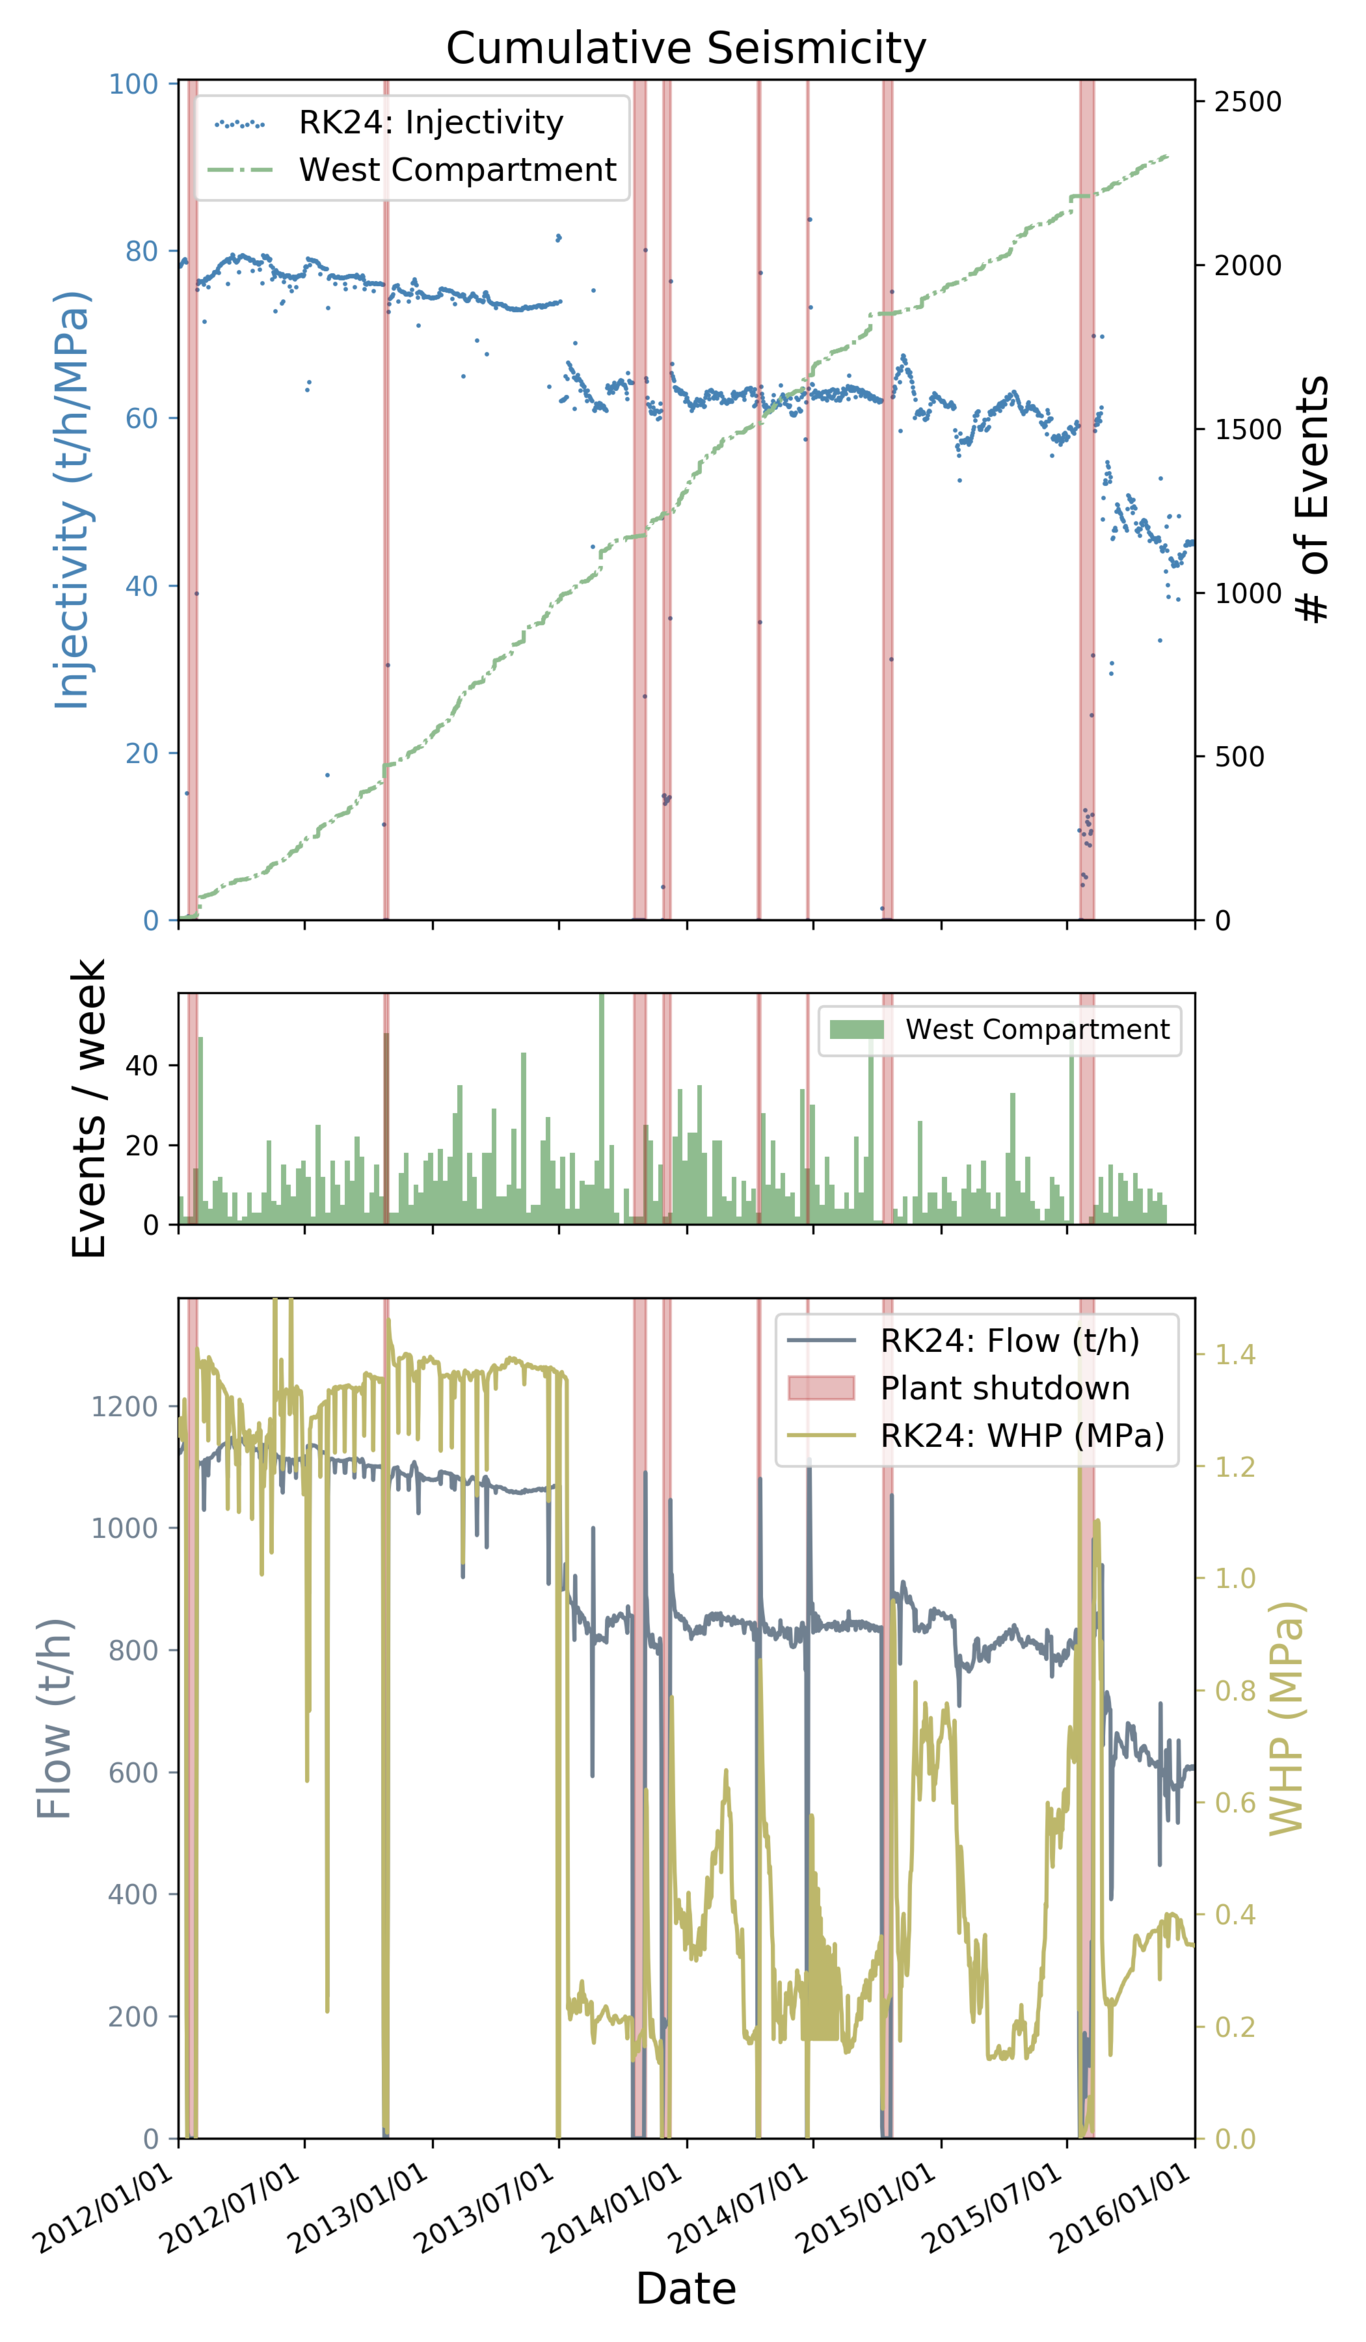
\includegraphics[width=0.75\columnwidth]{Chapter_4_Rot/figures/Rot_dets_GC_two_panel_WHP-flow_west_compartment_RK24/Rot_dets_GC_three_panel_II-rate-WHP_west_compartment_RK24}
\caption[Western compartment seismicity and RK24 injection parameters]{{
Seismicity in the western compartment defined above compared to well
parameters for well RK24. The top panel shows the cumulative number of
events (green dot-dashed) with \gls{injectivity} at RK24 (blue). The middle
panel shows the weekly rate of seismicity in the western compartment.
The bottom panel shows both \gls{flow_rate} (dark gray) and \gls{WHP_g}
(yellow). Red shaded regions in all panels indicate the periods during
which the power plants were shut down for maintenance, which have been
recognized previously as periods of potentially heightened seismicity.
{\label{108171}}%
}}
\end{center}
\end{figure}

The response of western compartment seismicity to the \gls{injectivity} decline and subsequent decrease in flow at RK24 is subtle or nonexistant. In addition, the drop in \acrshort{WHP} in July 2013 from $\sim${1.3} to 0.2 MPa does not produce the expected drop in the rate of seismicity. While the \gls{injectivity} decline, and in particular the subsequent pressure drop might be expected to produce significant changes in the character of seismicity, there are a number of reasons why this may not be the case. The most significant complication to interpretation is that RK24 is not the only injector in this part of the field. Even if the pressure signals between RK23 and RK24 are isolated by the \acrshort{IFF}, RK20 (on the same side of the fault as RK24) remained a significant injector throughout the dataset, injecting at a roughly constant rate of 600 t/h and a \gls{WHP_g} of approximately 0.4 MPa. This may have provided enough pressure support in this section of the reservoir to continue to induce seismicity at close to previous rates. In addition, even as pressure had dropped at RK24, the injection rate was still $\sim$800 t/h. As \citet{Sherburn_2015} and \citet{Sewell_2015WGC} have postulated, Rotokawa seismicity is likely affected more by stress changes induced by reservoir cooling than reservoir pressure increases, especially near the well. The results in Figure \ref{108171} support this view as seismicity seems insensitive to pressure perturbations of up to 1 MPa at the wellhead, which are normally more than sufficient to induce seismicity \citep{keranen2018induced,stein1999role}.

\subsection{RK23 halt and restart}
Most of the excess injection displaced by the RK24 \gls{injectivity} decline was accounted for by shallow injection into well RK12 (in the current production field) and deep injection into RK23. Prior to this, RK23 was being used as an injector for \acrshort{RGEN} condensate until late 2012, when it was shut for 8 months (gray bar, Figure \ref{102850}) before resuming injection, this time of \acrshort{NAP} brine \citep{Addison_2017stanford}. In Figure \ref{102850}, we plot characteristics of seismicity in the compartments that we interpret to be east of the \acrshort{IFF}, where the pressure signal from RK23 is assumed to be the strongest. Similar to the western compartment, the rate of seismicity is mostly constant over time. Interestingly, the northeast compartment, furthest from RK23, experienced an increase in the rate of seismicity during the 8 months when no injection was occurring at the well, whereas the southeast compartment did not. This increased rate of seismicity is still significantly lower than in the compartment near the well, but it is unclear why seismicity further from the well would respond more strongly to a pressure perturbation than seismicity nearer to the well.\selectlanguage{english}

\begin{figure}[p]
\begin{center}
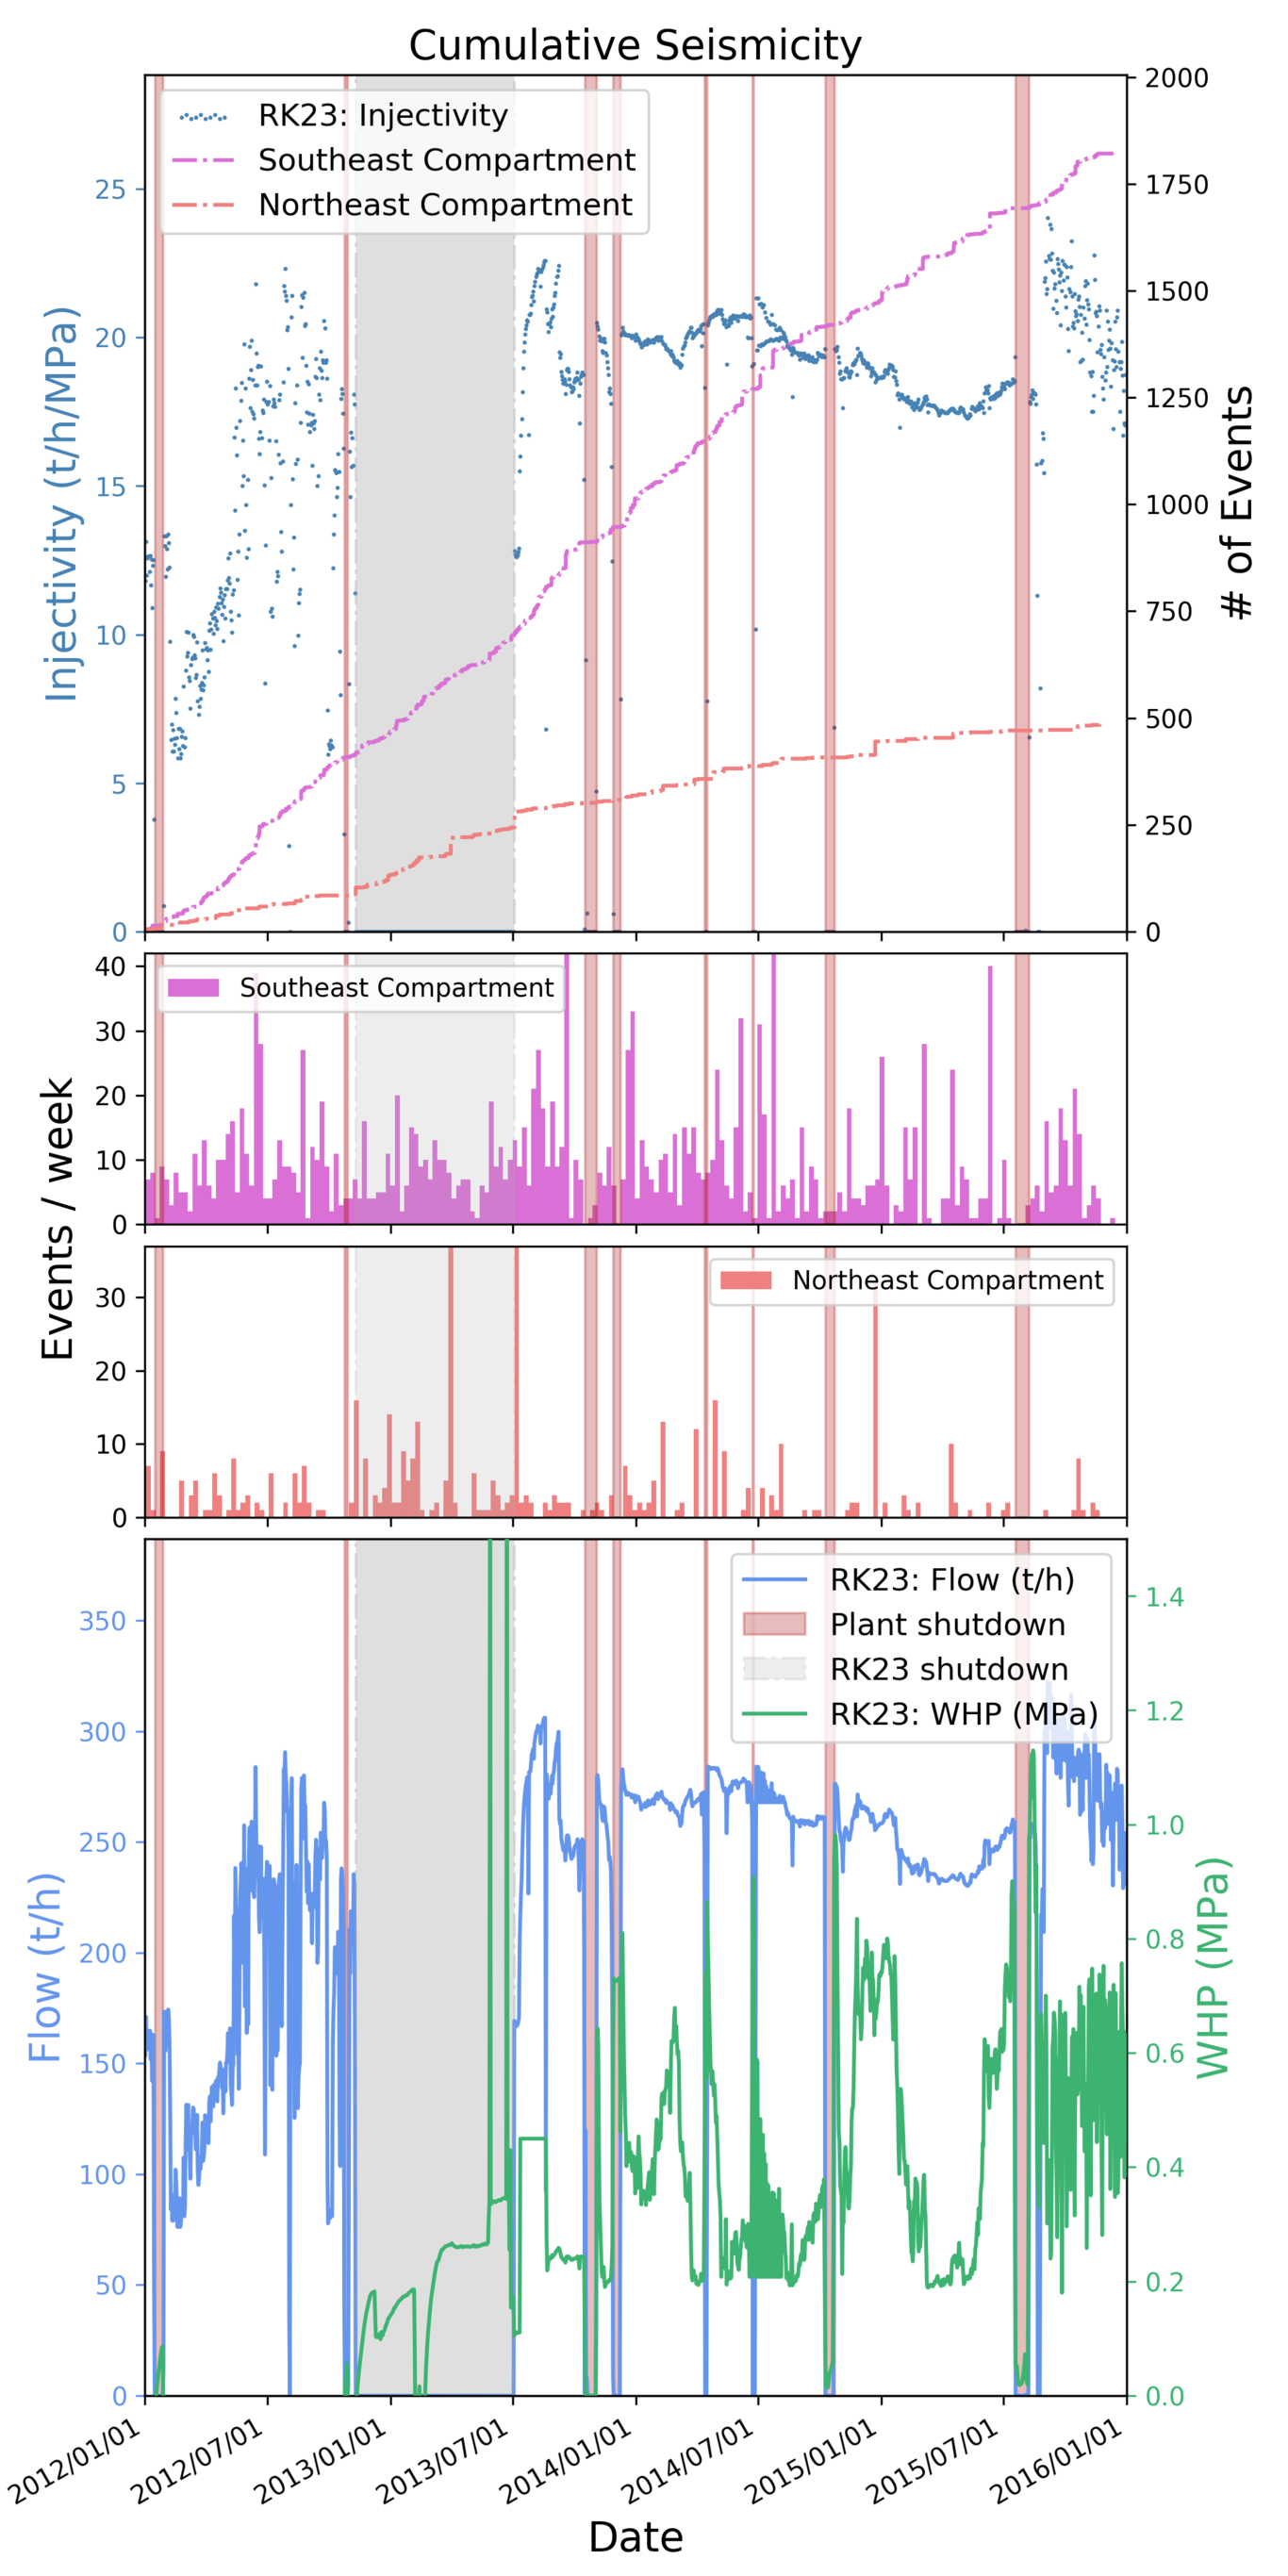
\includegraphics[width=0.63\columnwidth]{Chapter_4_Rot/figures/Rot_dets_GC_normalized_east_compartment_RK23_flow/Rot_dets_GC_four_panel_II-rate-WHP_east_compartment_RK23}
\caption[Eastern compartments' seismicity and RK23 injection parameters]{{
Seismicity in the eastern compartments defined above compared to well
parameters for RK23. The top panel shows the cumulative number of
events (magenta and coral colored lines) with \gls{injectivity} at RK23
(blue). The middle two panels show the weekly rate of seismicity in the
southeastern and northeastern compartments, respectively. The bottom
panel shows both \gls{flow_rate} (blue) and \gls{WHP_g} (green). Red
shaded regions in all panels indicate the periods during which the power
plants were shut down for maintenance, which have been recognized
previously as periods of potentially heightened seismicity. The period
of time during which RK23 was shut is shaded in gray.
{\label{102850}}%
}}
\end{center}
\end{figure}

\subsection{Aseismic injection: RK34 Drilling and RK21-22}
One new well, RK34, was drilled at Rotokawa during our study period. Although RK34 drilling incurred full fluid losses at reservoir depths, there was no discernible response in seismicity near the well, or anywhere else in the reservoir. This behavior is distinct from the similar case of NM10 drilling in Ngatamariki the year before, which induced a significant number of events \citep{j2019}. However, aseismic injection is not uncommon at Rotokawa or Ngatamariki in general \citep{Sewell_2015WGC}. For instance, drilling, and \gls{stimulation} at well NM09 in Ngatamariki was largely aseismic, and injection into the southwestern injection wells, RK21/RK22 at Rotokawa has historically been aseismic \citep{j2019,Sewell_2015WGC}.

The case of RK21-22 is particularly puzzling, because RK21 was used as the dominant injection well from NAP startup (\textgreater1000 t/h) until 2011, but seismicity has never been observed in this section of the field \citep{Sewell_2015WGC}. What's more, temperature and \gls{permeability} in RK21-22 are highly similar to RK20-24. Why, then, does seismicity occur at one and not the other? Modeling at the Geysers geothermal fields has shown that density driven, downward flow can drive stabilization of the reservoir fracture network in regions where $\sigma_{1}$ is vertical (such as at Rotokawa) \citep{Jeanne_2015tensor}. Although such an effect may help explain a lack of near-well seismicity in general, it does not explain the discrepancy between wells with such similar characteristics.

\section{Spatial $b$-value variations}\label{bvals}
Figures \ref{610416} and \ref{922043} reveal a complex pattern of $b$ within the Rotokawa reservoir that defies simple explanation. The higher $b$-value of the southeastern compartment as a whole, shown in Figure \ref{599295}c, is also discernible in Figure \ref{610416} (map view). However, $b$ is not uniform in space throughout any of the compartments. A profile of $b$-value for all compartments combined with distance from well RK23 or RK24 is shown in Figure \ref{922043}c.

If we use the inferred \acrshort{IFF} to divide the $b$-values into eastern and western compartments, on the basis that the pressure evolution on either side of the fault would be decoupled, the profiles take the shape of those in Figure \ref{922043}a and b. In the western compartment (Figure \ref{922043}b), $b$ generally decays with distance from the well out to approximately 1 km, as predicted by the geomechanical modeling of \citep{Bachmann_2012}, but increases from 1 km outwards. East of the \acrshort{IFF}, $b$-value behavior is even more complicated, increasing from $b\approx1.1$ near RK23, to $b>1.5$ at a distance of 650 m before decaying at greater distances.

Similar to \citet{Bachmann_2012}, we observe an increase in $b$ from the wellbore out to at least 150 m in all compartments. This may be an effect of near-well cooling, wherein the stabilization of the fracture network due to reservoir contraction counteracts the buildup in pore-pressure and suppresses failure on non-critically stressed fractures \citep{Jeanne_2015tensor}. With distance from the well, thermal cooling will decay more quickly than pore-pressure perturbation. This may lead to a situation in which cooling effects dominate near the well, acting to suppress $b$-value, but give way to pore-pressure perturbations further afield, thereby increasing $b$-value via the processes described by \citet{Bachmann_2012}.\selectlanguage{english}

For all compartments, $b$-value also shows a depth dependence wherein $b$ decreases from the surface to a minimum of $b\approx0.9$ at 2.5 km (roughly the depth of injection) and then increases with depth until the base of seismicity at roughly 4 km. This appears counterintuitive, given the currently-accepted reasoning that $b$-value is inversely proportional to differential stress ($\sigma_D$), which generally increases with increasing overburden at depth \citep{Schorlemmer_2005}. However, $b$-value has been shown to increase with depth in certain locations, especially in volcanic areas \citep[e.g.][]{Wiemer_1998}, perhaps owing to some combination of pervasive fracturing near intrusive bodies, high pore pressures, changing thermal gradients and an increase in host rock heterogeneity \citep{Schorlemmer_2005,Wiemer_1998,Warren_1970}. All of these characteristics are certainly present at Rotokawa, which image logs and well cuttings have revealed to be highly-fractured and geologically heterogeneous reservoir \cite{Massiot_2017,McNamara_2016}. However, very little is known about what lies beneath New Zealand geothermal fields, why they exist where they do or how they are fed \citep{Wilson_2016}. Evidence from drilling at Ngatamariki has shown that intrusive bodies do exist at depths \textless{3} km in the Taupo Volcanic Zone \citep{Chambefort_2016} and geochemical evidence suggests a similar intrusive body may sit below Rotokawa \citep{winick2009}. However, the true nature of the heat source is far from certain \citep{Wilson_2016}.

Unfortunately, it is difficult to make the case that geologic heterogeneity and the degree of fracturing increase with depth below the base of the reservoir, as the reservoir itself is already both heterogeneous and highly-fractured \citep{Massiot_2017,McNamara_2016}. What's more, pore-pressure perturbations originating at the injection wells decay with distance. This systematic decrease in $b$-value at reservoir depths may be a product of vertical contraction of the reservoir due to cooling, as suggested above. This would produce a preferential decrease in $\sigma_{1}$ ($\approx{\sigma_{V}}$ at Rotokawa), thereby decreasing the differential stress in the reservoir and counteracting the effect of pore-pressure buildup.

It is also possible that the depths presented for our catalog are systematically too deep, likely due to our lack of knowledge of the S-wave velocity structure in the field. Errors reported by bootstrap resampling of the input data used by \textit{GrowClust} indicate an average horizontal uncertainty of 200 m and an average depth uncertainty of 278 m. However, we relocated the catalog using only P-picks, and also using $V_{P}V_{S}$ ratios of 1.86 and 2.0 (compared to $V_{P}V_{S}=1.72$ presented here), all of which failed to change the depth dependence of $b$-value in the catalog. Once work is completed on a 3-D tomographic velocity model of the Ngatamariki and Rotokawa geothermal fields (by PhD student Steven Sewell), we may be better able to shed light on the depth uncertainties of seismicity at Rotokawa.\selectlanguage{english}

\begin{figure}[h!]
\begin{center}
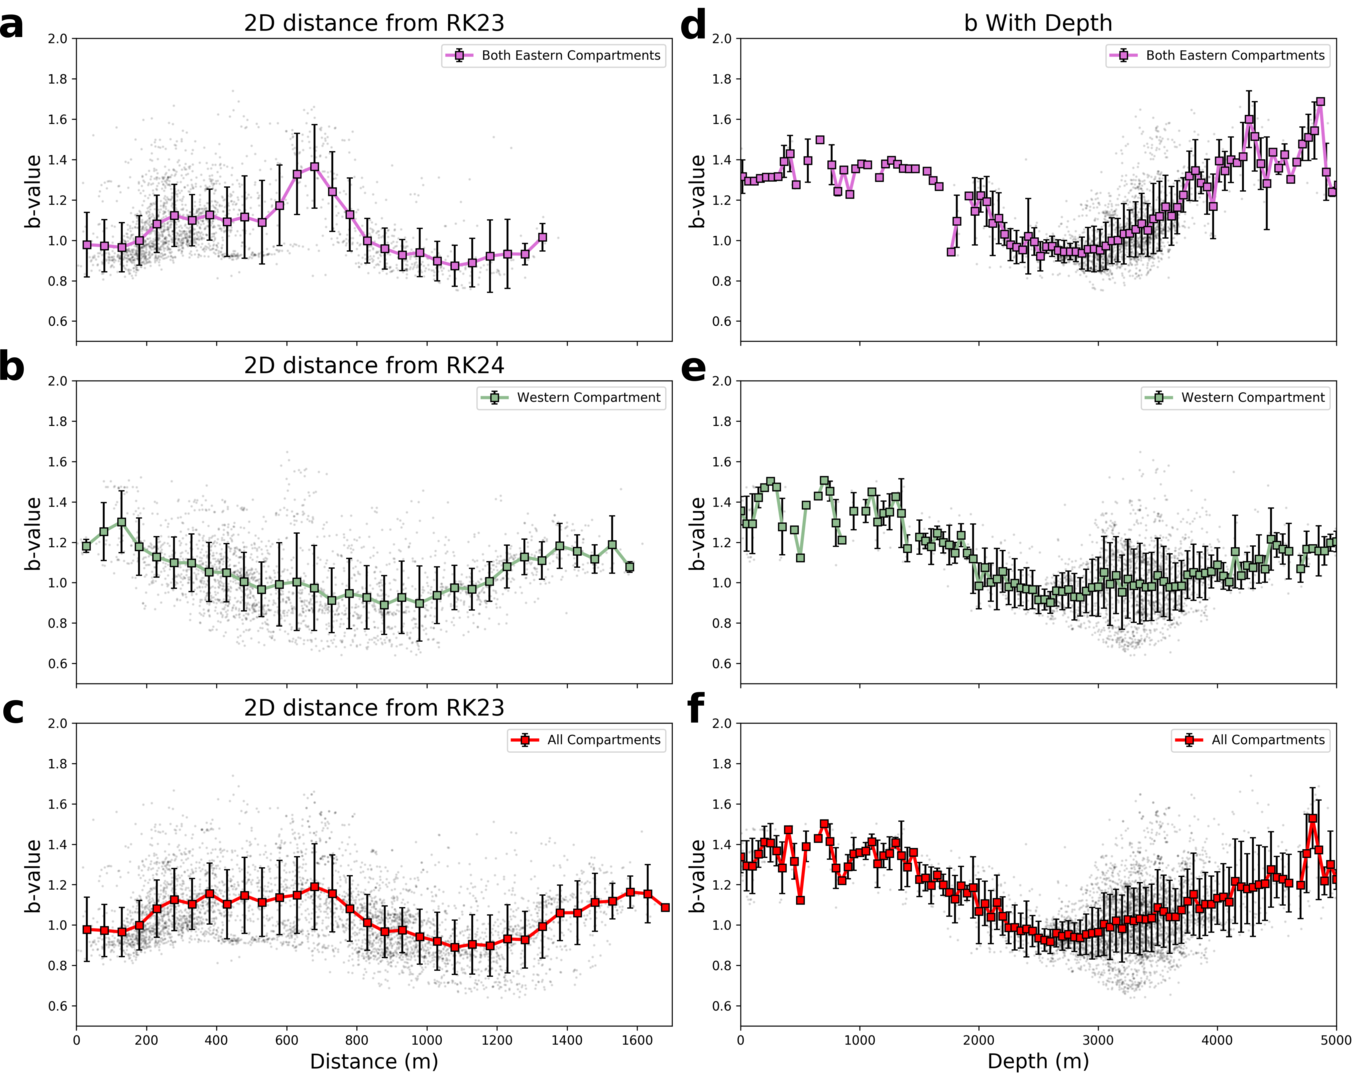
\includegraphics[width=0.98\columnwidth]{Chapter_4_Rot/figures/Rot_bval_w_radius_2D_RK23_min100_max300/Rot_bvalues_2D-depth_plots_2-17_labels}
\caption[Rotokawa $b$-value profiles with depth and event-well radius]{{
$b$-values with 2-dimensional radius from the bottom of injection well
RK23 (panels a and c) or RK24 (panel b).~ Panel a) shows the distance
from RK23 to all events in both eastern compartments, combined. Panel b)
shows the distance from well RK24 to all events in the western
compartment. Panel c) shows the distance from RK23 to all events in the
catalog. Markers show the average and bars show the standard deviation
in each distance bin. Panels d, e and f show the $b$-value distribution
with depth for the catalogs in panels a, b and c.
{\label{922043}}%
}}
\end{center}
\end{figure}

\section{Conclusions}
In this work, we analyze a four-year catalog of seismicity (2012--2015) for the Rotokawa geothermal field, corresponding to the four years immediately following the analysis of \citet{Sherburn_2015} and \citet{Sewell_2015WGC}. While seismicity during these four years is confined to the injection field, our catalog is able to identify structures within this compartment, revealing previously unknown compartmentalization in this part of the reservoir. The locations presented are able to further constrain the location and orientation of the Central Field Fault, and for the first time define the location of the Injection Field Fault, previously mapped only through vertical well cutting offsets and temperature gradients between wells. In addition, we have identified what may be a new structure, cutting across the dominant NE-SW structural grain. This structure may help explain the apparent pressure `leak' between the injection field and central production compartment identified by tracer testing \citep{Addison_2017stanford}, where previously no pressure support was identified.

Finally, we have mapped the magnitude-frequency distribution ($b$-value) in the reservoir. The pattern revealed is complex and fails to conform to a simplified model wherein $b$ decays exponentially with distance from a pressure source \citep{Bachmann_2012}. However, $b$ does show a significant contrast between the compartments revealed by hypocentral locations. Specifically, $b$ is higher to the east of the Injection Field Fault, suggesting that pressure may not be diffusing as readily in this section of the injection field, allowing non-critically stressed fractures to fail more often than in other compartments. It is possible that $b$-mapping at fields elsewhere could help to identify areas of the reservoir with large pressure gradients or changes in the degree of fracturing, which might exhibit as changes in the seismic $b$-value. In general, we believe these and other similar uses of earthquake magnitude information are under utilized as a tool for reservoir understanding and management.

\section{Appendices}
\subsection{`Swarm' activity}
\citet{Sewell_2015WGC} and \citet{Sherburn_2015} have observed periods of `swarm-like' activity (defined as days with \textgreater15 events) at Rotokawa that may coincide with pressure perturbations caused by plant maintenance shutdown and startup periods. To determine if such behavior is also present in our catalog, we have plotted red bars in Figures \ref{108171}, \ref{102850} and \ref{754214} indicating the times of plant shutdowns. The two shutdowns in 2012 (Figure \ref{754214}) appear to be associated with `swarm' events, defined here as days with more than 30 events due to the larger number of events in our catalog. However, the rest of the shutdowns appear to be anti-correlated with swarms periods with few events occurring while the plant is shutdown, as might be expected if we assume that events are purely induced by pore pressure increase.\selectlanguage{english}

\begin{figure}[h!]
\begin{center}
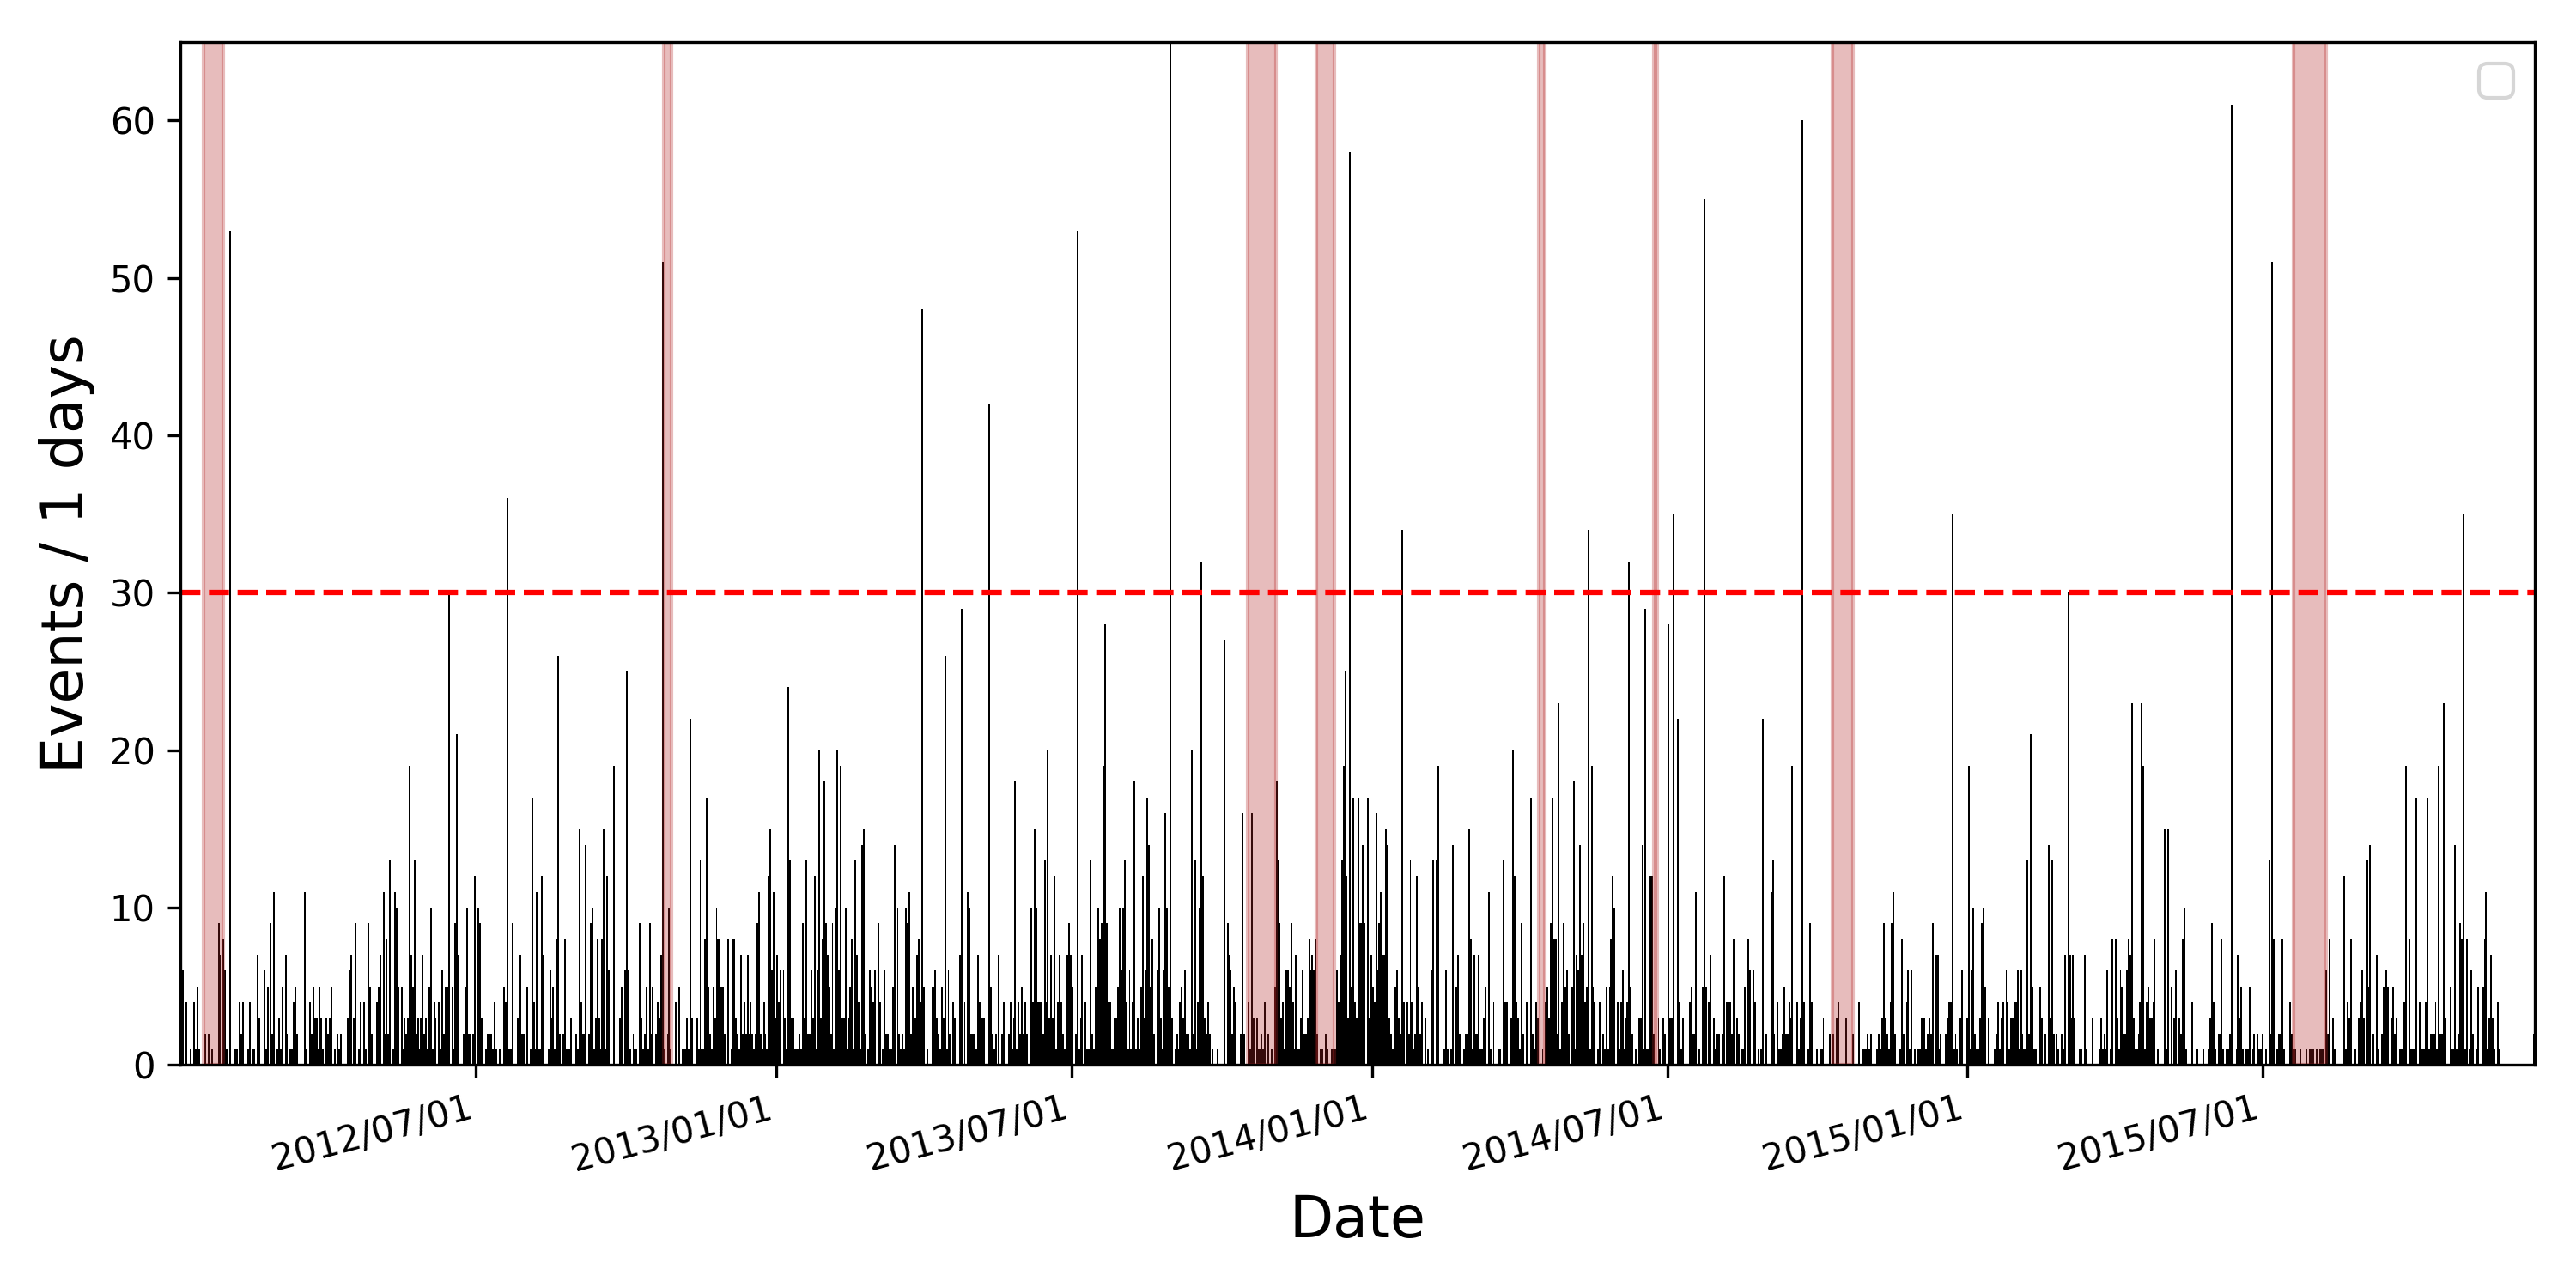
\includegraphics[width=0.98\columnwidth]{Chapter_4_Rot/figures/Rot_dets_rate_swarms/Rot_dets_rate_swarms_thresh_30_w_shutdowns_3-16}
\caption[Rotokawa `swarm' dates]{{
Daily rate of seismicity at Rotokawa. The red dotted line indicates the
threshold used to define the days corresponding to `swarm' events.
{\label{754214}}%
}}
\end{center}
\end{figure}

The location of swarm activity in our catalog is much the same as was reported by \citet[][Figure 5]{Sewell_2015WGC}, with events occurring preferentially along the \acrshort{CFF}, but with two other distinct clusters, one near RK23 and the other approximately 1 km to the north of RK23. The magnitude-frequency distribution of these events has a significantly lower $b$-value (0.77$\pm$0.03) (Figure \ref{322180}) than the catalog as a whole (1.09$\pm$0.02). We interpret the relative abundance of large-magnitude events as an indication that swarm events are indeed occurring preferentially on the \acrshort{CFF}, perhaps the only structure on which seismicity of M$_L$\textgreater3.0 (a rupture area of $\sim$0.1 km$^2$ \citep{stein_2000}) can occur within the field and which is optimally oriented for failure in the regional stress field.\selectlanguage{english}

\begin{figure}[h!]
\begin{center}
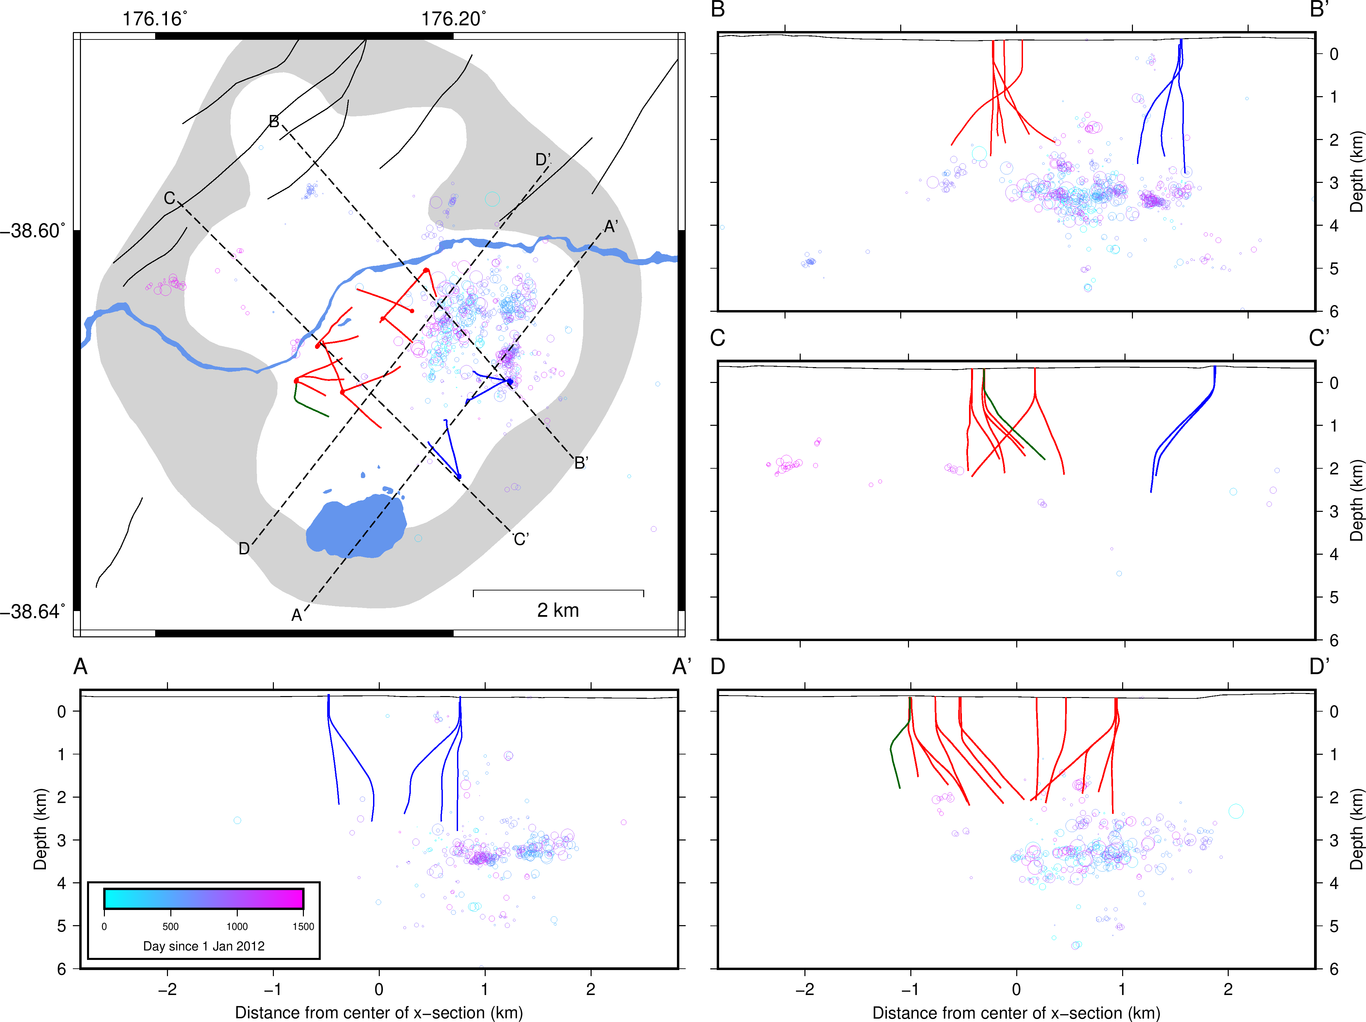
\includegraphics[width=0.98\columnwidth]{Chapter_4_Rot/figures/merc_Rot_dets_GC_swarms_30/merc_Rot_dets_GC_swarms_30}
\caption[Rotokawa `swarm' locations]{{
`Swarm-like' events at Rotokawa. Swarms were defined as days on which
more than 30 events occurred.
{\label{117000}}%
}}
\end{center}
\end{figure}\selectlanguage{english}


\begin{figure}[h!]
\begin{center}
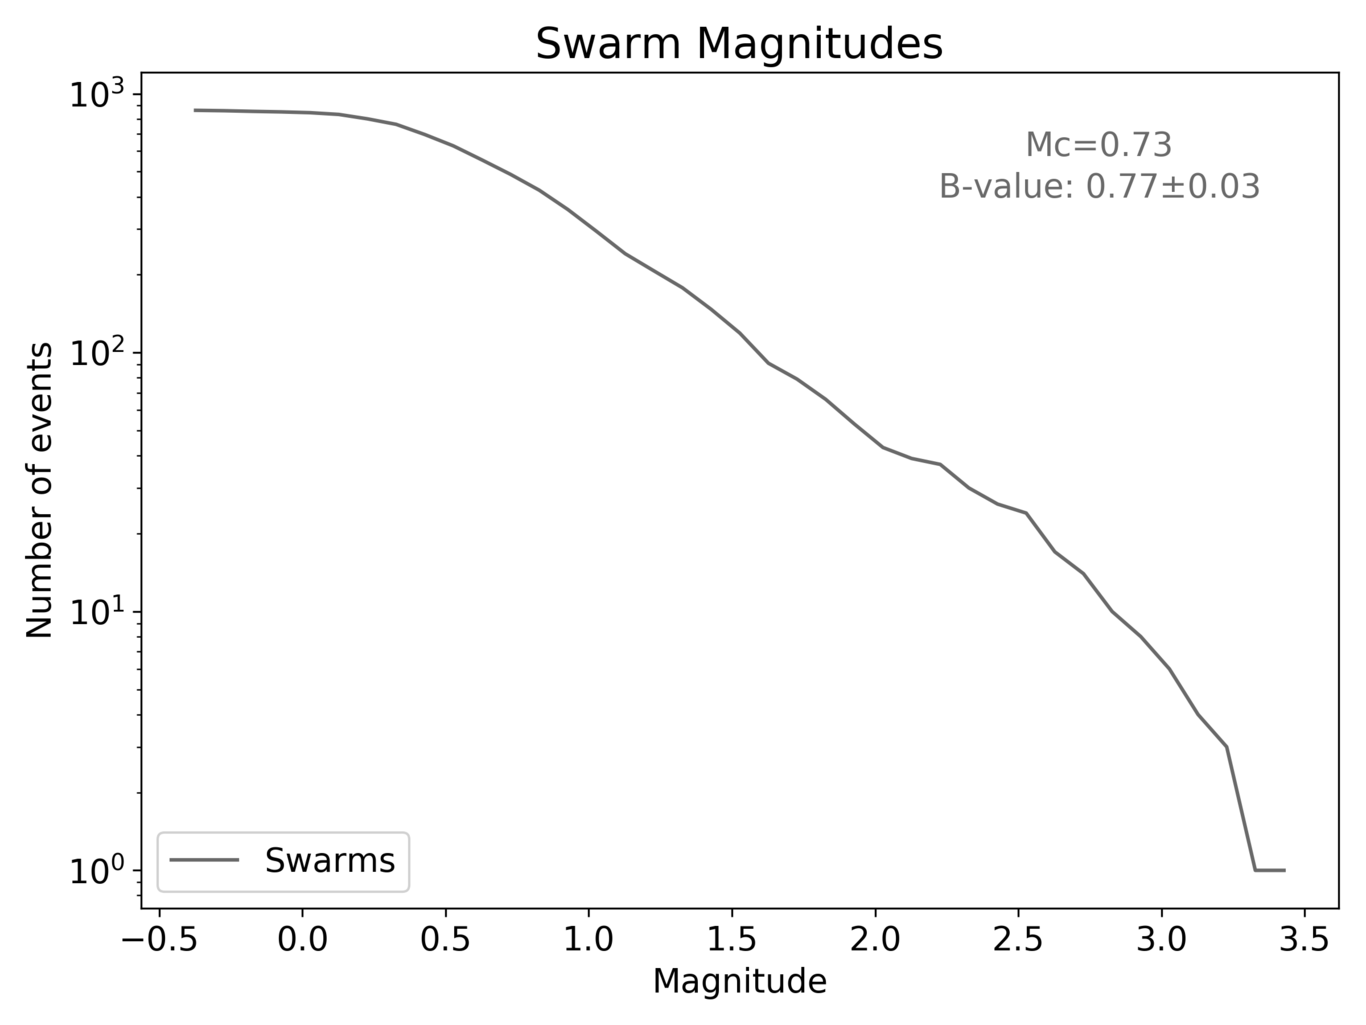
\includegraphics[width=0.70\columnwidth]{Chapter_4_Rot/figures/Rot_swarms_thresh_30/Rot_swarms_thresh_30}
\caption[`Swarm' frequency-magnitude distribution]{{
Frequency-magnitude distribution of events occurring on days of
heightened seismicity (i.e. `swarms').
{\label{322180}}%
}}
\end{center}
\end{figure}

% 	\cleardoublepage
% 	\chapter[Focal mechanisms and stress state at Rotokawa and Ngatamariki]{Focal mechanisms and stress state at \\Rotokawa and Ngatamariki}

\section*{Abstract}
Fluid injection and extraction activity has long been known to cause stress changes capable of inducing earthquakes. Typically, elevated pore-fluid pressure and extraction-induced poroelastic stress transfer are the causative mechanisms. However, at geothermal fields, thermal stresses induced by injecting cold water into a hot reservoir may play an under-appreciated and poorly understood role in changing the reservoir stress state. Here we present a catalog of focal mechanisms calculated from P-wave first motion polarities for two geothermal fields in New Zealand. We cluster these mechanisms based on distance and time before inverting for the stress state in the reservoirs, and make a case for reservoir cooling and contraction as the dominant mechanism responsible for changing stress in geothermal reservoirs. Routine inversion of similar focal mechanism datasets would allow geothermal operators to better constrain the geometry of flow pathways and therefore improve reservoir management and injection\slash{production} strategies.

\section{Introduction}
Although typically poorly understood, the state of stress within exploited reservoirs is of paramount importance in dictating flow pathways for hydrocarbon, heat and\slash{or} geothermal brine \citep{zoback2010}. Measuring the stress state in a reservoir located kilometers beneath the earth's surface is difficult and only possible in wells drilled to reservoir depth. The expense of drilling means that such wells are rare and intersect only small portions of a reservoir, leaving large volumes unsampled. As the reservoir stress state is known to vary laterally and with depth \citep{blake2011crustal,davidson_2012,McNamara_2015} on a scale of 100s of meters, stress variations likely go unnoticed away from and between wells.

When a reservoir is seismically active, earthquakes represent a manifestation of both fault\slash{fracture} orientation and the stress state which brought about slip on these fractures. Inversion of earthquake focal mechanisms can therefore be used to improve the stress picture in undrilled areas of the reservoir and can also provide information about the orientation of the fractures that host reservoir \gls{permeability}.

The Ngatamariki and Rotokawa geothermal fields are high-temperature ($\sim$300\textdegree{} C), liquid-dominated geothermal reservoirs in the Central Taup\={o} Volcanic Zone of New Zealand (Figure \ref{overview_Rot_Nga}), a zone of active extension and high-volume volcanism. Both fields are hosted in a thick succession of rhyolitic and andesitic volcanic flows, tuffs and ignimbrites with ages of \textless{2} Ma \citep{Wilson_1995,Wilson_2016}. Rotokawa has been used for power production since 1997 and Ngatamariki since 2012, between them producing roughly 220 \acrshort{MWe}.

\begin{figure}[h!]
\begin{center}
\includegraphics[width=1.00\columnwidth]{Chapter_5_FMs/figures/RotNga_overview/merc_RotNga_overview_struct}
\caption[Overview of the Ngatamariki and Rotokawa geothermal fields]{{
Overview map of the Ngatamariki and Rotokawa geothermal fields. Yellow polygons show the extend of each geothermal resource as defined by resistivity surveys \citep{Risk_2000,Boseley_2010}, black lines are mapped faults, and triangles are seismic stations used for this study. Within the fields, blue, red and green lines show the surface projection of injection, production and monitoring wells, respectively, with a circle indicating the location of the wellhead. Wells mentioned in the text are labeled in the inset panels. At Rotokawa, the modelled surface traces of the \acrfull{PFF}, \acrfull{CFF} and \acrfull{IFF} are plotted as dotted lines.
{\label{overview_Rot_Nga}}%
}}
\end{center}
\end{figure}\selectlanguage{english}

In this work we present a catalog of earthquake focal mechanisms solutions for both fields and use these catalogs to invert for the stress state. We attempt to address the resulting stress variations in space and time and comment on the potential relationships between power production (specifically fluid injection) and stress tensor variation. To our knowledge, this is the first study to use focal mechanism inversion to study stress state at a New Zealand geothermal field. However, the tectonic setting in the \acrshort{TVZ} is comparable to that at large geothermal fields elsewhere (e.g. The Geysers in northern California, USA) where extensive stress studies have been conducted using both high-quality focal mechanism inversions and coupled thermo-hydro-mechanical numerical simulations \citep[e.g.][]{Mart_nez_Garz_n_2013,Boyle_2014,Jeanne_2015tensor}. We refer to these studies to provide context for our results and suggest mechanisms for stress change in geothermal reservoirs in general.

\subsection{Stress changes at geothermal reservoirs}\label{stress_background}
In the last three decades, a number of workers have attempted to characterize the state of stress in geothermal reservoirs and determine the potential changes related to fluid injection and extraction activities \citep{oppenheimer1986extensional,feng1998microseismicity,sasaki2002determination,bohnhoff2004fault,Mart_nez_Garz_n_2013,Boyle_2014,Mart_nez_Garz_n_2014,Mart_nez_Garz_n_2017}. Although some of these studies were hampered by small amounts of data, the more recent works \citep[specifically][]{Mart_nez_Garz_n_2013,Boyle_2014,Mart_nez_Garz_n_2014,Mart_nez_Garz_n_2017} at The Geysers geothermal field in California were able to make use of large datasets of high-precision, well-constrained focal mechanisms ($n$\textgreater{6000} events) to invert for the principle stress axes in time and space.

Although starting from the same underlying dataset, \citet{Mart_nez_Garz_n_2013} and \citet{Boyle_2014} came to different conclusions from their stress inversion results. \citet{Boyle_2014} concluded that there was no discernible spatial deviation in the stress field related to injection\slash{extraction} activities at The Geysers, based on their observation that S$_{Hmax}$ was consistent both inside and outside of the reservoir, as well as at different depth intervals and spatial grid sizes. In contrast, \citet{Mart_nez_Garz_n_2013} determined that, at reservoir depths, They Geysers stress state is normal\slash{transtensional} and strike-slip\slash{transtensional} above and below. This is due to an apparent swapping of $\sigma_1$ and $\sigma_2$ dips at reservoir depths, leaving S$_{Hmax}$ unchanged (N15\textdegree{E}). It should be noted that, although \citet{Boyle_2014} concluded that power production activities had no effect on the stress state of the reservoir, their observations are not entirely inconsistent with those of \citet{Mart_nez_Garz_n_2013}, both of which show that S$_{Hmax}$ is unchanged throughout The Geysers.

Thermo-hydro-mechanical modeling of the stress-state response to injection at the Geysers \citep{Jeanne_2014,Jeanne_2015tensor} supports the interpretation of \citet{Mart_nez_Garz_n_2013}. They show that thermal contraction of the host rock at reservoir depths causes a variation in the dip of $\sigma_{1}$ at and below the depth of injection \citep{Jeanne_2015tensor}. This is because the injected fluid, which is much denser than the hot reservoir fluid, `sinks' to greater depths upon injection. This effect causes the cooled volume of the reservoir to take on a shape that is longer in the z (depth) direction than in the x or y direction, thereby reducing vertical stress more than the horizontal stresses. In their model, since $\sigma_{1}\approx{\sigma_{V}}$ at The Geysers (normal faulting regime), cooling reduction of $\sigma_{1}$ actually caused $\sigma_{1}$ and $\sigma_{2}$ (S$_{Hmax}$) to trade places after 7-8 months of injection, artificially inducing a strike-slip faulting regime within the reservoir \citep{Jeanne_2015tensor}. No such effect was observed when the same models were run in the absence of thermoelastic effects, indicating that these stress rotations are unique to injections where the temperature contrast between injected fluid and reservoir is high \citep{Jeanne_2015tensor}. 

These results likely apply directly to the development of the Ngatamariki and Rotokawa reservoirs, where the stress state and natural-state reservoir temperature are similar to The Geysers. 

\subsection{Fractures and stress state at Rotokawa and Ngatamariki}
At reservoir scale, structure at Ngatamariki and Rotokawa mirrors the NE-SW-striking trend of extensional faulting observed across the Taup\={o} Volcanic Zone. These NW- and SE-dipping antithetic structures accommodate the $\sim$5--15 mm/y of NW-SE regional extension \citep{Rowland_2004,Wallace_2004}. The only major structure to intersect both the Ngatamariki and Rotokawa reservoirs is the Aratiatia Fault Zone (Figure \ref{overview_Rot_Nga}). However, a number of other NE-SW structures of \textgreater{1} km in length have been inferred to exist within the fields \citep{wallis2013,Chambefort_2014}. Within the production and injection fields at Rotokawa, three major faults have been identified from geologic modeling of vertical offsets of well cuttings \citep{wallis2013}. From NW to SE these are the \acrfull{PFF}, \acrfull{CFF} and \acrfull{IFF} (Figure \ref{overview_Rot_Nga}).

If we consider the reservoirs at a scale of meters to 100s of meters, the orientation and extent of fracturing is mainly known through interpretation of borehole logs at selected wells (see Section \ref{data-methods}). At this scale, fracturing in the reservoirs exhibits the same NE-SW trend as the regional-scale faults. However, between wells and across both fields, the dominant dip of fracturing varies, likely controlled by the dip direction of the nearest large fault zone \citep{McNamara_2015}.

The TVZ is a zone of active extensional tectonics, with a stress state described by $\sigma_{1}\approx{\sigma_{V}}$ and S$_{Hmax}$ trending NE-SW \citep{Townend_2012}. Inversion of earthquake focal mechanisms has estimated the direction of S$_{Hmax}$ in the Central Taup\={o} Volcanic Zone to have an azimuth of $\sim$052--058\textdegree{} \citep{hurst2002earthquake,hurst2008characteristics}. Other estimates of the direction of S$_{Hmax}$ have been made from the orientation of drilling induced tensile fractures and other induced structures observed in borehole image logs at Rotokawa \citep{McNamara_2015}. For wells RK18L2, RK32 and RK30L1, estimates of S$_{Hmax}$ ranged from 025--049\textdegree{} \citep{McNamara_2015}. \citet{davidson_2012} also attempted to estimate the magnitudes of the principle stress components at Rotokawa but were hampered by a number of complexities with the data, including complex lateral variations in overburden and a lack of observed borehole breakout \citep{McNamara_2015}. No magnitude was estimated for S$_{Hmax}$ due to the lack of observed breakout, which \citet{davidson_2012} suggest was the result of the temperature range between drilling fluid and reservoir rock, suppressing the expansion of the borehole necessary to produce breakout. They were able to demonstrate that $\sigma_{V}$ and S$_{Hmin}$ ($\sigma_{3}$) at reservoir levels ($\sim$1100 m bsl) in Rotokawa vary laterally by up to 5 MPa over scales of less than a kilometer, similar to results presented for the Coso geothermal field in California \citep[e.g.][]{davidson_2012,blake2011crustal}.

\section{Data and methods}\label{data-methods}
\subsection{Earthquake catalog}
The earthquake catalog analyzed here was provided by GNS Science under contract with Mercury NZ, Ltd. Earthquake detection and location were conducted automatically using the \textit{SeisComP3} software package \citep{Weber2007}. We then revised the entire catalog manually, adjusting arrival times where warranted and picking P-wave first arrival polarities where possible. After removing all events with fewer than five polarity picks, 982 events remained. These events were separated into catalogs for each field (205 events for Ngatamariki, 777 for Rotokawa) and then incorporated into a large catalog of matched-filter detected events (\citet[described in detail by][]{j2019}). Finally, we relocated the entire catalog using the double-difference relocation program \textit{GrowClust} \citep{Trugman_2017}.

\subsection{Focal Mechanism Determination}\selectlanguage{english}
To calculate the focal mechanism solutions for this study, we used the Bayesian approach of \citet{Walsh_2009}, which allows the us to incorporate known uncertainties of the input parameters, specifically in hypocentral location and polarity picking error. Solutions were calculated using only manually-picked P-wave polarities, so long as a minimum of five picks were made per event. We calculated a total of 205 focal mechanism solutions at Ngatamariki and 777 at Rotokawa (Figures \ref{542095} and \ref{817909}). There are a median of seven polarity picks per event and an average standard deviation of the strike/dip/rake of 31.4\textdegree{}.

\begin{figure}[h!]
\begin{center}
\includegraphics[width=1.00\columnwidth]{Chapter_5_FMs/figures/merc_Nga_GC_focmecs/merc_Nga_GC_focmecs}
\caption[Ngatamariki focal mechanism solutions]{{
All calculated focal mechanisms for Ngatamariki from May 2012 until
November 2015. Grey polygons show the resistivity boundaries for
Ngatamariki (to the north) and Rotokawa (to the south). Black lines
indicate active faults from the GNS Active Fault Database \citep{AFDB} with the inferred orientation of the \acrshort{IFF} and \acrshort{CFF} drawn in bold and labeled. Red, blue and green lines indicate production, injection and monitoring wells. Focal mechanisms are colored by the
date of occurrence, with earlier events colored blue and later events
colored pink. Focal mechanisms have been reprojected in each
cross-section view to show ``back-hemisphere'' projections (i.e. the
hemisphere ``behind'' the panel). Each cross section shows only the
events within 1.5 km of the plane. Black triangles show the locations of
seismic stations.
{\label{542095}}%
}}
\end{center}
\end{figure}\selectlanguage{english}

As expected in the extensional TVZ, focal mechanisms at both fields show predominantly oblique normal faulting with subvertical P-axes. B-axis plunges are well distributed at Ngatamariki, showing no preference between pure normal and pure strike-slip faulting, whereas at Rotokawa, faulting is mostly normal with a minor oblique component (Figure \ref{FMC}). The mode of faulting at both fields appears to be unrelated to the hypocentral depth (Figure \ref{FMC}). 

\begin{figure}[h!]
\begin{center}
\includegraphics[width=1.00\columnwidth]{Chapter_5_FMs/figures/merc_Rot_GC_focmecs/merc_Rot_GC_focmecs}
\caption[Rotokawa focal mechanism solutions]{{
All calculated focal mechanisms for Rotokawa from May 2012 until
November 2015. The grey polygon shows the resistivity boundaries for
Rotokawa. Black lines indicate active faults from the GNS Active Fault
Database \citep{AFDB}, red lines indicate
production wells, blue lines indicate injection wells and the green line
is a reservoir monitoring well. Focal mechanisms are colored by the date
of occurrence, with earlier events colored blue and later events colored
pink. Focal mechanisms have been reprojected in each cross-section view
to show ``back-hemisphere'' projections (i.e. the hemisphere ``behind''
the panel). Each cross section shows only the events within 1.5 km of
the plane. Black triangles show the locations of seismic stations.
{\label{817909}}%
}}
\end{center}
\end{figure}

\begin{figure}[h!]
\begin{center}
\includegraphics[width=0.8\columnwidth]{Chapter_5_FMs/figures/FMC_plots/Merc_ALL_FMC_crop}
\caption[Kaverina diagrams of focal mechanism solutions at both fields]{{
Kaverina diagrams \citep{kaverina1996global,alvarez2014fmc} showing the kinematics for all focal mechanisms at Ngatamariki (top) and Rotokawa (bottom) based on the plunge of the B (null) and T axes for each event. Circles are scaled by magnitude and colored by depth.
{\label{FMC}}%
}}
\end{center}
\end{figure}

\subsection{K-means Clustering}
In order to investigate the spatial variation in the stress parameters at Rotokawa and Ngatamariki, we employ a `kmeans' clustering technique \citep{hartigan1975clustering}, based on the euclidian distances between all event pairs in the catalog. It is well known that the `kmeans' algorithm does not yield a unique solution to this clustering problem \citep[as noted by][]{Townend_2012}, but visual inspection of the results shows that no clusters violate logical divisions in the hypocenter distribution (across inferred faults, for example). We therefore have no reason to suspect that any particular cluster of samples multiple stress regimes, although this cannot be ruled out.

We divide the focal mechanisms at Ngatamariki (Figures \ref{542095}) into $k=$10 clusters and at Rotokawa (Figure \ref{817909}) into $k=$30 clusters, retaining only those clusters with 20 events or more. We performed the clustering over a range of $k$ values ($k=$5--30 at Ngatamariki; $k=$18--60 at Rotokawa) before selecting the value that maximized the number of groups at either field.

\subsection{Stress Inversion}
For each of the clusters established above, we inverted for the three principle stress axes ($\sigma_{1,2,3}$) and the stress ratio, $\nu$:
\begin{equation}
    \nu = \frac{\sigma_{1} - \sigma_{2}}{\sigma_{1} - \sigma_{3}}
\end{equation}
using the approach of \citet{Arnold_2007}. This approach allows us to readily incorporate the uncertainties in the focal mechanism parameters (strike/dip/rake) calculated using the approach detailed above and outputs a PDF of $\sigma_{1,2,3}$ and $\nu$. These can then be incorporated into the transformation of \citet{Lund_2007}, which returns an estimate of S$_{Hmax}$ for non-trivial cases where one principle stress is not vertical.

\section{Results}\label{results}
\subsection{Stress inversions}
\subsubsection{Ngatamariki}
At Ngatamariki, kmeans clustering for $k$=10 yielded five clusters of 20 events or greater (Figure \ref{nga_kmeans}), two in the north and three in the south. In the north, Cluster 2 is located nearest to injection well NM08 and contains mostly events that occurred during NM08 stimulation \citep{j2019}, while Cluster 6 includes events occurring adjacent to injection well NM09 (Figure \ref{nga_kmeans}).

The southern clusters, (4, 1 and 9 from the SW to NE, respectively), run along the strike of the Aratiatia Fault Zone with Cluster 1 centered at vertical injection well NM06 (Figure \ref{nga_kmeans}).

% Ngatamariki clusters fig
\begin{sidewaysfigure}[p]
\begin{center}
\includegraphics[width=0.8\textwidth,height=\textheight,keepaspectratio]{Chapter_5_FMs/figures/merc_Nga_GC_kmeans_10_GC_12-2-18/merc_Nga_kmeans_10_GC_12-2-18_intrusive}
\caption[Ngatamariki kmeans clusters]{{
Ngatamariki kmeans clusters ($k$=10) with 20 events or more. Red, blue and green lines represent production, injection and monitoring wells, respectively where the line is the well track and the square is the wellhead. The gray shaded area shows the resistivity boundary for the field \citep{Boseley_2010} and black lines indicate active faults \citep{AFDB}. In cross section, the dotted line at the bottom of the northern injection wells represents the top of the intrusive body (labeled `IB') as defined by well cuttings.
{\label{nga_kmeans}}%
}}
\end{center}
\end{sidewaysfigure}\selectlanguage{english}

\citep[][submitted]{j2019} performed stress inversions at Ngatamariki on a subset of the focal mechanisms analyzed here. The events they analyzed occurred during the \gls{stimulation} and completion testing of wells NM08, NM09 and NM10 in 2012-2013. They found that the stress state in southern Ngatamariki to be normal, with $\sigma_{1}\approx{\sigma_{V}}$ and S$_{Hmax}$ trending NE-SW at $\sim$045\textdegree{}. However, in the northern injection zone they found the stress regime to be inconsistent with regional normal faulting. There $\sigma_{1}$ dipped to the NE at $\sim$30\textdegree{} and $\sigma_{2}$\slash{}$\sigma_{3}$ formed a girdle, indicating a high stress ratio ($\nu$\textgreater{0.8}), where their respective orientations were difficult to distinguish. The discrepancy between the stress states in the northern and southern injection fields was attributed to the emplacement of a tonalite intrusive body in northern Ngatamariki, which may have significantly deviated the stress state.

We find a similar trend to \citep[][submitted]{j2019} when including all focal mechanisms from 2012-2015 (an increase in the number of focal mechanisms from 86 to 205) (Figure \ref{838980}). The additional events do not change the results of the inversions in southern Ngatamariki compared to the previous study, and a normal faulting regime still prevails. The three southern clusters (4, 1 and 9) progress along strike of the Aratiatia Fault Zone from near injection well NM10 in the southwest to past injection well NM06 in the northeast. There is little variation between the three inversions for these clusters. For each, $\sigma_{1}\approx{\sigma{_V}}$, S$_{Hmax}$ is oriented $\sim$045\textdegree and the stress ratio is low, $\nu=$0.3--0.4.

In the north, the stress state for Cluster 2 is unsurprisingly similar to the results presented by \citep[][submitted]{j2019}, given that most of the events in this cluster are common between the two datasets. Cluster 6 includes only events that have yet to be used for stress inversion. While Clusters 2 and 6 are only 300--400 m apart, the inversions reveal distinct stress states. In Cluster 2 $\sigma_{1}$ dips $\sim$30\textdegree{} at $\sim$020\textdegree{}, while it dips $\sim$51\textdegree{} at $\sim$090\textdegree{} in Cluster 6, forming a girdle with $\sigma_{2}$, indicating a stress ratio, $\nu$ approaching zero.

% Ngatamariki inversions fig
\begin{figure}[h!]
\begin{center}
\includegraphics[width=0.98\columnwidth]{Chapter_5_FMs/figures/Nga_kmeans_inversion_10/Nga_temps_GC_dets_kmeans_10_transparent_colored}
\caption[Ngatamariki stress inversions from kmeans clusters]{{
Lower hemisphere stereonets representing the stress inversion results for each k-means cluster shown in Figure~{\ref{nga_kmeans}}. Red corresponds to $\sigma_{1}$, green to $\sigma_{2}$ and blue to $\sigma_{3}$, where the filled circle represents the maximum likelihood axis and the contours represent the shape of the PDF for that axis. The black dotted line shows the direction of maximum horzontal compressive stress (S$_{Hmax}$) for which the gray shaded bowtie shows the 90\% confidence region. Each plot is annotated below with the calculated stress ratio, $\nu$. Stereonet backgrounds are colored-coded to match the corresponding cluster in Figure~{\ref{nga_kmeans}}.
{\label{838980}}%
}}
\end{center}
\end{figure}

\subsubsection{Rotokawa}
At Rotokawa, the hypocenters for the focal mechanisms shown in Figure \ref{817909} reveal the same two NE-SW striking structures discussed in Chapter 4, which we continue to interpret as being the \acrfull{CFF} and \acrfull{IFF} from west to east, respectively. As these structures are known to act as cross-strike barriers to fluid flow, we choose to divide the reservoir into distinct `compartments' bounded by these structures (Figure \ref{878143}). Our chosen kmeans clustering parameter, $k$=30, produced 14 clusters, each containing a minimum of 20 focal mechanism observations. We then group these clusters into compartments as follows:

\begin{itemize}
\item{The western compartment (light green, Figures \ref{878143} and \ref{434168}), contains all clusters northwest of the \acrshort{IFF} and southeast of the \acrshort{CFF}. These are Clusters 7, 2, 9, 12 and 17, shown in Figure \ref{434168}}
\item{The southeastern compartment (pink, Figures \ref{878143} and \ref{434168}), contains clusters southeast of the \acrshort{IFF} and south of the cross-strike structure inferred from the offset in focal mechanism locations along strike of the \acrshort{IFF}. These are Clusters 0, 3, 25, 13, 14, and 15, shown in Figure \ref{434168}}
\item{The northeastern compartment (coral, Figures \ref{878143} and \ref{434168}), contains the remainder of the clusters southeast of the \acrshort{IFF} (Clusters 10 and 23, Figure \ref{434168}).}
\item{The final cluster, Cluster 28, is located just inside the northern production field. We infer the centroid of this cluster to be outside the bounds of the compartments described above.}
\end{itemize}

% Rotokawa clusters fig
\begin{sidewaysfigure}[p]
\begin{center}
\includegraphics[width=0.75\textwidth,height=\textheight,keepaspectratio]{Chapter_5_FMs/figures/merc_Rot_GC_dets_kmeans_30/merc_Rot_kmeans_dets_30_comps}
\caption[Rotokawa kmeans clusters]{{
Rotokawa kmeans clusters ($k$=30) with greater than 20 events. Red and blue lines represent production and injection wells, respectively. The gray shaded area shows the resistivity boundary for the field \citep{Risk_2000} and black lines indicate active faults \citep{AFDB}. The colored polygons show the boundaries for the three inferred `compartments' defined in Chapter 4 based on linear features revealed in by earthquake hypocenters. The western compartment is green, southeastern pink and northeastern coral. These colors are used to map the polygons shown here in map view to the results presented in Figures \ref{434168} and \ref{237918}. 
{\label{878143}}%
}}
\end{center}
\end{sidewaysfigure}\selectlanguage{english}

Figure \ref{434168} shows the stress inversion results for each cluster, divided by compartment and color coded to match Figure \ref{878143}. From a first glance, it is clear that each inversion shows a normal faulting regime, with $\sigma_{1}\approx{\sigma_{V}}$. Only minor variations in the plunge of $\sigma_{1}$ are observed, but these are within the bounds of focal mechanism uncertainties ($\sim$30\textdegree{} angular deviation of the P axis).

Figure \ref{434168} also shows stress inversions that include all focal mechanisms in each compartment (white background, labeled `ALL'). In the western compartment, S$_{Hmax}$ is oriented 056\textdegree{} while in the northeast compartment, S$_{Hmax}$ is oriented 053\textdegree{}. For both of these compartments, $\nu$ approaches 1. In the southeast compartment, S$_{Hmax}$ is oriented 021\textdegree{} with a $\nu$ of 0.65. It is important to note that as the values of $\nu$ approach 1.0 throughout most of the reservoir, uncertainty in S$_{Hmax}$ also increases due to the ambiguity in the orientations of $\sigma_{2}$ and $\sigma_{3}$.

% Rotokawa kmeans inversions fig
\begin{sidewaysfigure}[p]
\begin{center}
\includegraphics[width=\textwidth,height=\textheight,keepaspectratio]{Chapter_5_FMs/figures/Rot_kmeans_inversion_30/Rot_temps_GC_dets_kmeans_30_compartments_combined_lores}
\caption[Rotokawa stress inversions from kmeans clusters]{{
Lower hemisphere stereonets representing the stress inversion results for each k-means cluster shown in Figure~{\ref{878143}}. Red corresponds to $\sigma_{1}$, green to $\sigma_{2}$ and blue to $\sigma_{3}$, where the filled circle represents the maximum likelihood axis and the contours represent the shape of the PDF for that axis. The black dotted line shows the direction of maximum horzontal compressive stress (S$_{Hmax}$) for which the gray shaded bowtie shows the 90\% confidence region. Each plot is annotated below with the calculated stress ratio, $\nu$. Stereonets are grouped into three colored boxes indicating the compartment in which they are located. These boxes are color coded to match the compartment boundaries in Figure \ref{878143}. The stress inversion results using all focal mechanisms in each compartment are the solutions with the white background to the right of each box (labelled `ALL').
{\label{434168}}%
}}
\end{center}
\end{sidewaysfigure}\selectlanguage{english}

% Discussion
\section{Discussion}
\subsection{Ngatamariki}
\subsubsection{Stress inversion}\label{nga_stress_results}
The relatively small number of focal mechanisms calculated for Ngatamariki (205) precludes the extensive clustering that would allow us to analyze temporal variations in the stress state at the reservoir, as has been done elsewhere \citep[e.g.][]{Mart_nez_Garz_n_2013}. The five clusters shown in Figures \ref{nga_kmeans} and \ref{838980} reveal spatial variations similar to those found by \citep{j2019}. As expected, the three clusters in the southern injection field show a normal faulting regime with NE-SW S$_{Hmax}$, consistent with all previous studies of stress in the region \citep{hurst2002earthquake,hurst2008characteristics,Townend_2012}. The stress ratio, $\nu$, in Cluster 1, closest to the main injection well, NM06, is lower than in Clusters 4 or 9 (0.3 as compared to 0.4), but the uncertainties overlap considerably, and we therefore will not comment on their significance.

In the Ngatamariki northern injection zone, both Cluster 2 and 6 indicate a strongly deviated stress regime with no vertical principle stress. Between the two clusters, both $\nu$ and S$_{Hmax}$ vary considerably. S$_{Hmax}$ is 022\textdegree{} and 066\textdegree{} at Clusters 2 and 6, respectively, while $\nu$ is 0.8 and 0.1. The striking contrast between these two clusters, with cluster centroids located \textless{1} km apart, is puzzling. \citet{j2019} suggest that the tonalite intrusive body, encountered in both well NM08 and NM09, may be responsible for the deviation of the northern Ngatamariki stress state from an expected normal regime. The geometry and orientation of this intrusive is poorly constrained, with cutting found in only three wells \citep{Chambefort_2014}, making it difficult to assess its effect on stress locally. Unless it is highly irregularly shaped (e.g. a series of dikes/sills) we envision the intrusive having a similar effect on the stress state at both Cluster 2 and 6, which are located at similar depths and similar distances to the top of the intrusive. However, stress variations due to irregularities in the shape and orientation of the intrusive body (or bodies) provide the simplest explanation for the change in stress between the two clusters.

We foresee two other possible explanations for the contrast between Clusters 2 and 6 that are related to elevated pore-fluid pressure and\slash{or} reservoir cooling caused by fluid injection. The events belonging to Cluster 2 are likely related to injection into the nearest well, NM08, while those in Cluster 6 are located at the position of the \glspl{feedzone} of NM09. It is possible that differences in the injection parameters at NM08 and NM09 could explain the stress variation. However, as shown in Figure \ref{clust26}, \glspl{WHP_g} at both wells are modest during our study period (\textless{2} MPa). As pore-pressure acts equally on each of the principle stress components, such large deviations in $\nu$ and S$_{Hmax}$ are unlikely to be pore-pressure related. 

\begin{figure}[h!]
\begin{center}
\includegraphics[width=0.84\columnwidth]{Chapter_5_FMs/figures/clust_2-6_comparison/NgaN_ALL_kmeans10_clusters_flow}
\caption[Ngatamariki Clusters 2 and 6 relative to injection flow rate]{{
Northern Ngatamariki \glspl{flow_rate}, \glspl{WHP_g}, and focal mechanisms. Cluster 2 (red) and Cluster 6 (orange) are shown as stems with the plan view lower-hemisphere focal mechanism solution as a head and the height corresponding to the magnitude of the event. Although the clusters were created via kmeans clustering based on euclidian distance between events, the clusters are also perfectly split in time with Cluster 2 occurring early in the study period, and Cluster 6 occurring later.
{\label{clust26}}%
}}
\end{center}
\end{figure}

As mentioned in Section \ref{stress_background}, thermoelastic stress reduction near injection wells can produce large deviations in the local stress state \citep{Jeanne_2015tensor}. While the simplest explanation for the contrast in stress between Clusters 2 and 6 is related to the intrusive body, we believe that reservoir contraction due to cold water injection presents a compelling alternative explanation. The degree to which a reservoir with fracture-dominated \gls{permeability} contracts in response to cold water injection is related to a number of factors that describe both the reservoir (e.g. rock bulk modulus and fracture spacing) as well as the injection itself (injectate temperature and \gls{flow_rate}) \citep{stephens1982hydraulic}. Although the injectate temperature at both wells is similar, the rate of injection is not. NM08 is less permeable than NM09 and, as a result, accepts only $\sim$250 t/h as compared to the nearly 1100 t/h injected at NM09 (Figure \ref{clust26}) resulting in total injected volumes over our study period of 4.19e6 m$^3$ and 2.07e7 m$^3$, respectively. We would therefore expect the cooling-related stresses at NM09 to be more significant than at NM08.

However, it is worth emphasizing that the majority of events in Cluster 2 occurred during the \gls{stimulation} of NM08 (duration of one month) and not over the entire study period (Figure \ref{clust26}). As these events occurred $\sim$200 m from the main \glspl{feedzone} at NM08, thermal \gls{diffusivity} (measured in mm$^2$/s \citep{Kanamori_1968}) and short duration of \gls{stimulation} make it unlikely that they were influenced by cooling from the well. In contrast, the events in Cluster 6 are well-distributed over a longer period and are therefore more likely to have been influenced by thermoelastic stresses. The extent of reservoir cooling has been confirmed by \acrshort{PTS} runs at monitoring well NM02 ($\sim$250 m from NM09), where temperatures at reservoir depths had cooled by $\sim$100\textdegree C within 3 years of the start of injection (Steve Sewell, personal comm.). Therefore, the cooling zone extending from NM09 likely encompasses most of the events in Cluster 6 and likely extends further towards the production field, although it has not yet reached well NM07 (Figure \ref{nga_kmeans}). We can be confident that the stress inversion of Cluster 6 is therefore affected by thermoelastic stresses.

If the cooled zone around NM09 is larger in the vertically than it is laterally (picture a pipe oriented vertically), it will have reduced $\sigma_{1}$ by more than $\sigma_{2}$ or $\sigma_{3}$. Such a scenario may help explain the lower stress ratio and different faulting regime observed in Cluster 6 when compared with Cluster 2. A similar phenomenon was observed and modeled by \citet{Jeanne_2015tensor,Mart_nez_Garz_n_2013} at The Geysers, where a normal faulting regime above and below the reservoir has become a strike-slip regime within it as a result of cooling at the injection wells.

\subsection{Rotokawa}
\subsubsection{Spatial stress variation}
As demonstrated in Figure \ref{434168}, deviations in stress state at Rotokawa are somewhat less dramatic than between northern and southern Ngatamariki. For each of the clusters at Rotokawa, $\sigma_{1}\approx{\sigma_{V}}$, with only minor variations in dip that cannot be confidently resolved. However, there are spatial variations in both S$_{Hmax}$ and $\nu$ that deserve further inspection. Specifically, values for S$_{Hmax}$ and $\nu$ in the southeast compartment, nearest the injection wells, are distinct to those in other parts of the field (Figure \ref{434168}).

Borehole measurements of drilling-induced tensile failure in the production field (RK18L2, RK32, RK30L1) \citep{McNamara_2015} show that S$_{Hmax}$ ranges from 025--049\textdegree{}. They also demonstrate that lateral stress changes in the reservoir are significant and can occur over distances of \textless{1} km. However, as no images were obtained from any of the current injection wells, we have little constraint on the orientation of stress or fractures in the seismically active part of the field. Inverting for the stress state using all mechanisms in the southeast compartment, S$_{Hmax}$ is 021\textdegree{} with a stress ratio, $\nu$, of 0.65. For all mechanisms in the western compartment, S$_{Hmax}$ is 056\textdegree{} and $\nu$ approaches 1, while in the northeast compartment S$_{Hmax}$ is 053\textdegree{} and $\nu$ also approaches 1. These values for S$_{Hmax}$ are roughly consistent with directions obtained from the borehole measurements \citep{McNamara_2015}.

In Figure \ref{533041} we show the stress inversion results projected onto the horizontal plane as bowties showing the 90\% confidence interval for S$_{Hmax}$, colored by the stress ratio. While it is tempting to interpret the apparent anticlockwise rotation of S$_{Hmax}$ in the southeast compartment (relative to the rest of the field) as related to injection well proximity, there are a number of caveats. Most importantly, stress ratios approaching 1.0 in the rest of the reservoir suggest that $\sigma_{2}$ and $\sigma_{3}$ have similar magnitudes. Given that $\sigma_{2}$ and $\sigma_{3}$ are horizontal here, stress inversion from focal mechanisms cannot adequately resolve the true direction of S$_{Hmax}$ for a stress ratio of 1. So while an azimuth of 021\textdegree{} for S$_{Hmax}$ in the southeast compartment is relatively well constrained, interpreting it in the context of S$_{Hmax}$ throughout the rest of the reservoir is unwarranted.

Although stress ratio is the least well-resolved parameter resulting from the inversion of focal mechanisms, we can at least say with some confidence that $\nu$ is lower, on average in the southeast compartment than in the rest of the reservoir. As the southeast compartment contains, or is adjacent to, injection wells RK20, 23 and 24, it is subject to some of the highest pore pressures and temperature gradients in the field. As discussed for Ngatamariki, it is difficult to envision a scenario in which elevated pore pressures of $\sim$1 MPa would deviate the in situ stress state in any discernible way, especially given that pore pressure affects each principle stress axis equally. A decrease of 1 MPa for all principle stress axes will change the stress ratio by some small amount, but this is unlikely to be measurable through focal mechanism inversion.

Instead, we believe the only injection-related process capable of producing significant stress changes at Rotokawa is the cooling of the reservoir host rock. As injection had been occurring in the current configuration (i.e. at wells RK20--24) for at least five years by the end of our study period, the cooling front would have had time to reach the boundaries of our inferred southeast compartment, and likely the southern portions of the western compartment as well. Numerical modeling of The Geysers geothermal field in California has shown that stress reductions measured in 10's of MPa are possible over time spans of 2--5 years for similar injectate temperatures and in situ stress state to what is encountered at Rotokawa \citep{Jeanne_2015tensor}. These stress changes are greatest directly adjacent to the wells, as would be expected, because there the fluid is coldest and the induced thermal gradient is the greatest. As the cool, denser fluid enters the reservoir, it flows downward, driven by gravity. This gravity flow results in a vertically elongate zone of cooling, which preferentially reduced whichever stress axis is most vertical \citep{Jeanne_2015tensor}. In the case of The Geysers, Rotokawa and Ngatamariki, this means preferential reduction of $\sigma_{1}$, which has the effect of limiting the population of fractures oriented for failure and reducing the stress ratio. As the injected fluid begins to heat and flow laterally, the zone of cooling also elongates in the direction of greatest lateral \gls{permeability}, likely subparallel to S$_{Hmax}$, along strike of structures such as the \acrshort{IFF} or \acrshort{CFF}, which are well oriented for failure in the regional stress regime. We envision a complex interplay between the state of stress and the geometry of the zone of cooling at Rotokawa, where faults that are well-oriented for failure also define a preferred axis of cooling. It is possible that preferential reduction of $\sigma_{1}$ due to gravity-driven flow in the southeastern compartment has led to a reduced stress ratio in this portion of the field and that a limited degree of cooling further from the wells has left the stress state largely unchanged.

% Rotokawa SHmax figure
\begin{figure}[h!]
\begin{center}
\includegraphics[width=0.84\columnwidth]{Chapter_5_FMs/figures/merc_Rot_kmeans_cents_40_sigmas_seis_nu/merc_Rot_dets_kmeans_30_cents_SHmax_nu_comps}
\caption[S$_{Hmax}$ and $\nu$ for kmeans clusters at Rotokawa]{{
S$_{HMAX}$ directions for the kmeans clusters (Figure \ref{878143}) at Rotokawa. Bowties show the 90\% confidence intervals for S$_{Hmax}$, colored by the stress ratio, $\nu$.
{\label{533041}}%
}}
\end{center}
\end{figure}


\subsubsection{Temporal stress variation}
Finally, we compare stress parameters from focal mechanism inversion to temporal changes in injection at Rotokawa. Due to the vertical $\sigma_{1}$ and high stress ratio in the western and northeastern compartments, S$_{Hmax}$ is poorly constrained and we therefore avoid further subdividing these areas for temporal analysis. In the southeast compartment, the calculated stress ratio is lower than elsewhere in the field and S$_{Hmax}$ is better constrained. Its proximity to injection wells means that this compartment is also the most likely to show signs of injection-induced stress change. We therefore divide the 304 focal mechanisms in this compartment into time-sequential groups of 55 events, and invert for the stress states in each group, advancing the inversion by steps of 10 events between data points. As $\sigma_{1}\approx{\sigma_{V}}$ for all clusters at Rotokawa, we plot S$_{Hmax}$ and $\nu$ with time versus the injection rates from RK20, 23 and 24 (Figure \ref{IFF_temporal}). 

\begin{figure}[h!]
\begin{center}
\includegraphics[width=0.84\columnwidth]{Chapter_5_FMs/figures/Rot_IFF_temporal/IFF_wedge_nu_Shmax_w_time_win55_ol45_RK20-23-24}
\caption[S$_{Hmax}$ and $\nu$ with time near injection wells at Rotokawa]{{
Stress inversions in the southeastern compartment at Rotokawa with time. Each data point corresponds to a cluster of 55 consecutive focal mechanisms with an overlap of 45 events between adjacent data points. Points are plotted at the time average for each subset of events. The lower panel shows \glspl{flow_rate} for injection wells RK20, 23 and 24 during the study period.
{\label{IFF_temporal}}%
}}
\end{center}
\end{figure}

Both S$_{Hmax}$ and $\nu$ appear to respond to the injection changes at wells RK23-24 during the last half of 2013. $\nu$, in particular, decreases from near 1.0 to below 0.2 over the six months following the injection shift from RK24 to RK23. If our interpretation of the orientation of the \acrlong{IFF} is correct, and it also serves as a barrier to cross strike flow, then the stress state to the east of the \acrshort{IFF} would respond most strongly to RK23, which is the only well on the eastern side of the fault. If this is the case, then the decrease in $\nu$ and anticlockwise rotation of S$_{Hmax}$ shown in Figure \ref{IFF_temporal} may correspond to the restart in injection at RK23 after $\sim$8 months of inactivity. As described in Section \ref{nga_stress_results}, such a decrease in $\nu$ could reflect preferential cooling of $\sigma_{1}$ (Figure \ref{cooling}). This makes sense in the context of a well that has been inactive for a number of months. During this time, the near-well reservoir would have had ample time to re-heat to near the natural state temperature. Once injection restarted (Figure \ref{cooling}a), the temperature contrast would have encouraged gravity-driven, downward flow from the well and a corresponding decrease in $\nu$. Interestingly, $\sim$7 months after the restart of injection at RK23, $\nu$ began to rebound, eventually returning to elevated levels (\textgreater{0.8}) by the end of the study period. The steep drop and more gradual rebound of $\nu$ may tell us something about the time scale and geometry of reservoir cooling. If a decrease in $\sigma_{1}$ corresponds to the drop in $\nu$ due to downward flow, perhaps the rebound in $\nu$ reflects a transition from downward to lateral flow (Figure \ref{cooling}b), likely along fractures subparallel to $\sigma_{2}$ (S$_{Hmax}$). As flow transitions from gravity-driven to lateral, the shape of the cooled zone of the reservoir changes from a sub-vertical cone beneath the well to one with a larger lateral footprint. If lateral \gls{permeability} is anisotropic, favoring flow in the direction of S$_{Hmax}$, as we would expect, then the zone of cooling would also be elongate in this direction, thereby cooling S$_{Hmax}$ more than $\sigma_{3}$ (Figure \ref{cooling}b). Such a scenario could produce an increase in $\nu$ similar to what we observe in the southeast compartment at Rotokawa.

% cooling schematic
\begin{sidewaysfigure}[p]
\begin{center}
\includegraphics[width=0.65\textwidth,height=0.8\textheight,keepaspectratio]{Chapter_5_FMs/figures/cooling_schematic/res_cooling_schematic}
\caption[Effect of thermoelastic cooling on the reservoir stress state]{{
Cartoon illustrating a possible scenario for stress ratio ($\nu$) variations with time in the southeast compartment at Rotokawa. \textbf{a)} density-driven flow of cold injectate at the outset of injection, much like what may have occurred at RK23. As injection starts, the cooled zone of the reservoir is larger in the vertical dimension than in any horizontal dimension. This produces a preferential reduction of the principle stress that is most vertical. In a normal faulting regime, such as at Rotokawa, this produces a reduction of $\sigma_{1}$, as well as a reduction of differential stress and a reduction in stress ratio, $\nu$. \textbf{b)} After some years of injection (right panel), the injected fluid begins to spread laterally in the direction of greatest \gls{permeability} (i.e. subparallel to $\sigma_{2}$). As this happens, the stress reduction of $\sigma_{2}$ outpaces that of $\sigma_{1}$, the horizontal footprint of the cooled zone grows and stress ratio increases. We envision such a mechanisms to explain the oscillatory behavior of $\nu$ observed in the southeast compartment at Rotokawa, following the restart of injection at RK23. 
{\label{cooling}}%
}}
\end{center}
\end{sidewaysfigure}

If our interpretation is incorrect, and RK23-24 inject into the same pressure compartment, then it may be difficult to distinguish the contribution of each well to variations in stress. In this case, RK20 and 24 may also contribute to the temperature and pressure variations in the southeast compartment and the observed decrease in $\nu$ may also be related to the decrease in flow at RK24.

\section{Conclusions}
In this work we present 982 focal mechanisms calculated from P-wave first motion polarities for the Ngatamariki (205) and Rotokawa (777) geothermal fields in the Central Taup\={o} Volcanic Zone of New Zealand. Mechanisms at both fields are predominantly normal and strike-slip events, with small or insignificant reverse components. We have divided this catalog into various spatial and temporal clusters and inverted each for the stress tensor, seeking to determine how stress varies across the fields and assess possible relations to fluid injection activities.

Using a kmeans spatial clustering approach, we created five clusters at Ngatamariki and 14 at Rotokawa, each with a sufficient number of focal mechanisms to reliably determine the stress state from the cluster. At Ngatamariki, we show that the stress state is distinct between the northern and southern injection zones, with a normal faulting regime in the south (S$_{Hmax}\approx{}$ NE-SW) and an oblique normal faulting regime in the north with no vertical principle stresses. There are too few events at Ngatamariki to divide the catalog into meaningful temporal clusters and it is therefore difficult to comment on the effects of fluid injection on the stress state. However, it may be possible to explain the spatial variation in the stress inversions for Clusters 2 and 6 in the northern injection zone via reservoir cooling processes.

At Rotokawa, the large number of focal mechanisms (777) allows for better spatial and temporal resolution from our stress inversions. Although the stress results here show exclusively normal faulting ($\sigma_{1}\approx{\sigma_{V}}$) for all clusters, spatio-temporal variations in the direction of S$_{Hmax}$ and stress ratio, $\nu$, suggest that injection operations may be affecting the stress state. In particular, temporal variations in stress state, specifically $\nu$, for a subset of events nearest the injection wells indicate that this parameter may be sensitive to variations in injection \gls{flow_rate}. We suggest that this may reflect variations in the size and geometry of the cooled zone of the reservoir around the wells.

The findings presented here constitute the first published study of the stress variation in the Ngatamariki field and the first attempt to characterize stress from focal mechanisms at Rotokawa. The results confirm the expected first-order normal faulting regime with NE-SW S$_{Hmax}$ at both fields but show significant variation in space, especially at northern Ngatamariki where the stress field varies significantly from the south. From an operational point of view, the knowledge of the stress state away from logged wells aids in identifying the population of fractures that are well-oriented for failure, and therefore the most likely to host fluid flow. This knowledge is critical for planning injection and production strategies and for targeting wells.

\section{Appendices}
\subsection{AFIT and FMI logs}
Borehole image logs use either the variations in electrical resistivity (Formation Micro Imager: FMI) or amplitude variations in acoustic reflections off the borehole wall (AFIT: Acoustic Formation Imaging Technology) to construct an image of the well with a resolution of \textless5--10 mm \citep{massiot2015processing,McNamara_2015}. Structures intersecting the wellbore appear as sinusoids in the unwrapped image, from which the orientation of individual fractures, bedding planes and geologic contacts can be determined \citep{massiot2015processing}. For the two available FMI logs (wells NM09 and NM10), we report only `non-halo', conductive fractures as reported by \citet{nm09_report} and \citet{nm10_report}, which have the highest likelihood of being open and not filled with a sealing mineral such as pyrite or calcite. These are the strongest candidate fractures for hosting fluid flow in the reservoir, and accommodating seismic slip. The remaining logs referenced in this work were collected via AFIT, and are therefore unable to distinguish between sealed and unsealed fractures \citep{massiot_2012,massiot2015processing}. For AFIT logs, we report all fractures of both high and low confidence identified in the well log reports \citep{massiot_2012,massiot_rk18l2,massiot_rk32,mcnamara2011rk29,mcnamara2010rk30l1}.

At Ngatamariki, logs were collected at wells NM08 and NM09, in the northern injection zone, and well NM10 in the southern injection zone \citep{massiot_2012,nm09_report,nm10_report}. While the dominant strike across all wells in the field is NE-SW, dips differ between wells. Fractures in NM08 strike $\sim$030\textdegree{} and dip to the SE at an average of $\sim$65\textdegree{}, while those in NM09, $\sim$200 m to the Southeast, strike $\sim$211\textdegree{} and dip NW at $\sim$60\textdegree{}. This likely indicates the presence of antithetic structures, one intersecting NM08, dipping southeast, and the other intersecting NM09 dipping northwest \citep{massiot_2012,nm09_report}. Fractures at NM10 strike an average of $\sim$008\textdegree{} and dip $\sim$62\textdegree{} with more dipping to the southeast than northwest. There are also two subordinate strikes at NM10, one at $\sim$360\textdegree{} and another at $\sim$260\textdegree{}. The bimodal dip distribution and complex distribution of strikes likely reflect the complex structure within the Aratiatia Fault Zone, into which NM10 is drilled (Figure XX).

At Rotokawa, well logs were taken for four wells in what is now the production field: RK18L2, RK32, RK30L1 and RK29 \citep{massiot_rk18l2,massiot_rk32,mcnamara2011rk29,mcnamara2010rk30l1}. As at Ngatamariki, the majority of fractures strike NE-SW but dip in accordance with the nearest large structure (i.e. \acrshort{PFF}, \acrshort{CFF}, \acrshort{IFF}). Dips at well RK18L2, RK30L1 and RK29 are to the northwest at $\sim$69\textdegree{}, $\sim$71\textdegree{} and $\sim$68\textdegree{}, striking $\sim$199\textdegree{}, $\sim$223\textdegree{} and $\sim$161\textdegree{}, respectively. Fractures at RK32, nearest the \acrlong{PFF}, strike an average of $\sim$052\textdegree{} with a dip of $\sim$70\textdegree{}SW.

\subsection{Borehole vs focal mechanism fracture orientation}
To accompany the stress work detailed in the main body of this chapter, we have also used focal mechanism solutions to characterize the orientation of the fracture network within the area of active seismicity. This is of critical importance to geothermal operators as the orientation of open fractures reveals aspects of the flow pathways from injection to production wells. Improved understanding of these pathways allows reservoir engineers to better plan injection and production strategies in order to minimize cooling and pressure drawdown.

While focal mechanism solutions are described equally well by two orthogonal nodal planes, we can calculate which is the most likely to fail for a given stress regime. Failure increases fracture \gls{permeability} through misalignment of asperities on opposing fracture faces (a process known as self-propping). Therefore, by calculating the fractures which are best oriented for failure in a given stress regime, we are also determining the fractures which are most likely to provide pathways through which reservoir fluid will flow.

Figures \ref{237918} and \ref{237919} compare the orientations of fractures measured from borehole imaging with those inferred from the most likely failure planes from the focal mechanisms analyzed above. In order to determine which plane was the most likely to fail, we used the approach of \citet{vavryvcuk2014iterative}, who define the instability of a plane as:

\begin{equation}
I = \frac{\tau - \mu(\sigma - 1)}{\mu + \sqrt{1 + \mu^{2}}}
\end{equation}

where $\tau$ and $\sigma$ are the shear and normal tractions on a given plane, respectively and $\mu$ is the coefficient of static friction. We invert all focal mechanisms for the stress tensor at each field separately. We then use the whole-field stress result to calculate the least stable planes for each focal mechanism in the corresponding field.

% Ngatamariki fractures fig
\begin{sidewaysfigure}[p]
\begin{center}
\includegraphics[width=\textwidth,height=\textheight,keepaspectratio]{Chapter_5_FMs/figures/Nga_fracture_FM/ALL_fracs_and_FMs_Ngatamariki}
\caption[Ngatamariki fracture orientations and focal mechanism nodal planes]{{
Ngatamariki fracture orientations measured from acoustic (NM08-NM09) or resistivity (NM10) imaging of boreholes, compared with the least stable nodal planes for each of the focal mechanisms in this study. The instability criterion used to decide which plane was most likely to fail was based on the approach of \citet{vavryvcuk2014iterative}.
{\label{237918}}%
}}
\end{center}
\end{sidewaysfigure}\selectlanguage{english}

In Figures \ref{237918} and \ref{237919}, we have divided both the well imaging results and focal mechanisms into the major spatial clusters for comparison. In Ngatamariki we divided the data into northern and southern injection wells and the corresponding focal mechanisms clusters (Figure \ref{237918}). The image logs for northern wells NM08 and NM09 have highly uniform fracture orientations striking NE-SW, dipping SE at NM08 and NW at NM09. The most likely nodal planes also show a preference for NE-SW strike in this portion of the reservoir, albeit mostly dipping W-NW. In northern Ngatamariki there is also a subordinate, SSE-striking, WSW-dipping population of nodal planes that do not appear in the wellbore image logs. The reasons for this discrepancy are unclear, although there is a large degree of scatter in the fracture populations measured at the wells, which means that SSE-stiking fractures do exist in the wells, albeit in relatively limited numbers.

% Rotokawa fractures fig
\begin{sidewaysfigure}[p]
\begin{center}
\includegraphics[width=\textwidth,height=\textheight,keepaspectratio]{Chapter_5_FMs/figures/Rot_fracture_FM/ALL_fracs_and_FMs_Rotokawa}
\caption[Rotokawa fracture orientations and focal mechanism nodal planes]{{
Rotokawa fracture orientations measured from acoustic imaging of boreholes, compared with the least stable nodal planes for each of the focal mechanisms in this study. The instability criterion used to decide which plane was most likely to fail was based on the approach of \citet{vavryvcuk2014iterative}.
{\label{237919}}%
}}
\end{center}
\end{sidewaysfigure}\selectlanguage{english}

At Rotokawa, the image logs were collected only at wells in the production field, which therefore do not correspond directly to the area of active seismicity. We divided the focal mechanisms into the western (green), southeastern (pink) and northeastern (coral) compartments discussed above and color-coded the rose plots based on the convention established in Figures \ref{878143}, \ref{434168} and \ref{533041}. For reference, the western compartment is the compartment closest to the wells for which image logs were collected (specifically RK29 and RK30L1). With that context, the image log results at RK29 and RK30L1 compare favorably with the most-likely nodal planes in the western compartment, which exhibit SSE strikes and WSW dips with small subordinate orientations of E striking, S dipping and SW-striking, NW-dipping fractures and nodal planes. Although it contains fewer focal mechanisms and is located further from the logged wells, the northeast compartment exhibits a similar nodal plane distribution to the western compartment. In contrast, the southeast compartment shows a much wider distribution of likely nodal plane orientations with a dominant orientation of NNE-striking, ESE-dipping fractures. We interpret this well-distributed population of unstable fractures as an indication of elevated pore-pressures in this injection-adjacent compartment of the reservoir. Elevated pore pressures should have the effect of broadening the distribution of fractures that are critically stressed in a given stress regime, which has been suggested for injection operations elsewhere \citep[e.g.][]{Bachmann_2012}. We think this approach to fracture network characterization can be applied to sets of focal mechanisms at geothermal reservoir elsewhere and paired with the stress determination detailed above to better understand the orientation of flowing fractures and \gls{permeability} away from wells.
% 	\cleardoublepage
% 	\include{Chapter_6_Synthesis/}
% 	\cleardoublepage

% Make the glossary
\printglossary[type=\acronymtype,title={Abbreviations and units}]
\printglossary

% Now appendices
\begin{appendices}
% \include{Appendices/}

%%%NO NEED TO INCLUDE ELECTRONIC SUPPLEMENTS INTO TABLE OF CONTENTS
%\include{Appendix_Electronic/Appendix_TLScloud}
%\include{Appendix_Electronic/Appendix_RKdata}
%\include{Appendix_Electronic/Appendix_DFDPdata}

\end{appendices}
\backmatter

% Bibliography
\bibliographystyle{agufull}
\bibliography{Chaps1-4_pinned_citekey}
\end{document}